\documentclass[11pt]{book}
\oddsidemargin 0in
\evensidemargin 0in
\marginparwidth 0in
\textheight 8in
\textwidth 6.5in
\topmargin 0in
\headheight 14pt
\usepackage{amssymb,amsmath,amsthm,fancyhdr,supertabular,longtable,hhline,mathtools}
\usepackage{colortbl}
\usepackage{import, multicol,boxedminipage}
\usepackage{chapterfolder}
\usepackage[metapost,truebbox]{mfpic}
\usepackage[pdflatex]{graphicx}
\usepackage{makeidx}
\usepackage[colorlinks, hyperindex, plainpages=false, linkcolor=blue, urlcolor=blue, pdfpagelabels]{hyperref}
\usepackage[all]{hypcap}
\usepackage{cancel}
\usepackage{sectsty}
\usepackage{textcomp}
\allsectionsfont{\mdseries \scshape}
\definecolor{ResultColor}{gray}{0.9}
\theoremstyle{definition}  % this prevents the text in definitions, theorems, and corollaries from being italicized
\newtheorem{defn}{\sc Definition}[chapter]
\newtheorem{thm}{\sc Theorem}[chapter]
\newtheorem{cor}[thm]{\sc Corollary}
\newtheorem{eqn}{\sc Equation}[chapter]
\newtheorem{ex}{\sc Example}[section]
\newtheorem{fig}{\sc Figure}[chapter]
\setlength{\parindent}{0in}
\newcommand{\bbm}{\begin{boxedminipage}{6.41in}}
\newcommand{\ebm}{\end{boxedminipage}}
\usepackage{array}
\setlength{\extrarowheight}{2pt}
\allowdisplaybreaks[2]
\allsectionsfont{\mdseries \scshape}
%Below is for Helvetica (scaled): 
\usepackage[scaled=.92]{helvet}   
\renewcommand{\familydefault}{\sfdefault}  %makes the text of the book sans serif
\usepackage[helvet]{sfmath}  %makes the math in the book sans serif
\allsectionsfont{\sffamily}  %makes the chapter and section titles sans serif

\makeatletter
\newcases{mycases}{\quad}{%
  \hfil$\m@th\displaystyle{##}$}{$\m@th\displaystyle{##}$\hfil}{\lbrace}{.}
\makeatother

\begin{document}
\newcounter{HW}
\newcounter{HWindent}
\renewcommand{\textinterrobang}{$! \! \! ?$}


\chapter{\sc Exponential and Logarithmic Functions}

\section{Exponential Functions}

\mfpicnumber{1}

\opengraphsfile{ExponentialFunctions}

\setcounter{footnote}{0}

\label{ExponentialFunctions}

Of all of the functions we study in this text, exponential  functions are possibly the ones which impact everyday life the most. This section introduces us to these functions while the rest of the chapter will more thoroughly explore their properties. 

\smallskip

 Up to this point, we have dealt with functions which involve terms like $x^3$,  $x^{\frac{3}{2}}$, or $x^{\pi}$ -  in other words, terms of the form  $x^{p}$ where the base of the term, $x$, varies but the exponent of each term, $p$, remains constant.  
 
 \smallskip
 
 In this chapter, we study functions of the form $f(x) = b^{x}$ where the base $b$ is a constant and the exponent $x$ is the variable.  We start our exploration of these functions with the time-honored classic,  $f(x) = 2^{x}$.  
 
 \smallskip
 
 We make a table of function values, plot enough points  until we are more or less confident with the shape of the curve,  and connect the dots in a pleasing fashion.

\hspace{1in} \begin{tabular}{m{2.7in}m{3in}}

\setlength{\extrarowheight}{4pt}
\[ \begin{array}{|r||r|r|}  

\hline

 x & f(x) & (x,f(x)) \\ \hline
-3 & 2^{-3} = \frac{1}{8} & \left(-3, \frac{1}{8} \right) \\ [2pt] \hline
-2 & 2^{-2} = \frac{1}{4} &  \left(-2, \frac{1}{4} \right) \\ [2pt] \hline
-1 & 2^{-1} = \frac{1}{2} &  \left(-1, \frac{1}{2} \right) \\ [2pt]  \hline
0  & 2^{0} = 1 & ( 0 ,1) \\  \hline
1  & 2^{1} = 2 & ( 1, 2) \\  \hline
2  & 2^{2} = 4 & (2,4) \\  \hline
3  & 2^{3} = 8 & (3, 8) \\  \hline
\end{array} \] 
\setlength{\extrarowheight}{2pt}

&

\begin{mfpic}[13]{-4}{4}{-1}{9}

\axes
\tlabel[cc](4,-0.5){\scriptsize $x$}
\tlabel[cc](0.5,9){\scriptsize $y$}
\tcaption{\scriptsize $y = f(x) = 2^{x}$}
\xmarks{-3,-2,-1,1,2,3}
\ymarks{1,2,3,4,5,6,7,8}
\tlpointsep{4pt}
\axislabels {x}{{\scriptsize $-3 \hspace{7pt}$} -3, {\scriptsize $-2 \hspace{7pt}$} -2, {\scriptsize $-1 \hspace{7pt}$} -1, {\scriptsize $1$} 1, {\scriptsize $2$} 2, {\scriptsize $3$} 3}
\axislabels {y}{{\scriptsize $1$} 1, {\scriptsize $2$} 2, {\scriptsize $3$} 3, {\scriptsize $4$} 4, {\scriptsize $5$} 5, {\scriptsize $6$} 6, {\scriptsize $7$} 7, {\scriptsize $8$} 8}
\penwd{1.25pt}
\arrow \reverse \arrow \function{-3.5, 3.1, 0.1}{2**x}
\point[3pt]{(-3,0.125), (-2,0.25), (-1,0.5), (0,1), (1,2), (2,4), (3,8)}
\end{mfpic} \\

\end{tabular}

A few remarks about the graph of $f(x) = 2^{x}$ are in order.  As $x \rightarrow -\infty$ and takes on values like $x = -100$ or $x=-1000$, the function $f(x) = 2^{x}$ takes on values like $f(-100) = 2^{-100} = \frac{1}{2^{100}}$ or $f(-1000) = 2^{-1000} = \frac{1}{2^{1000}}$.  

\smallskip

In other words, as $x \rightarrow -\infty$, $2^{x} \approx \frac{1}{\text{very big $(+)$}}  \approx \text{very small $(+)$}$   That is, as $x \rightarrow -\infty$, $2^{x} \rightarrow 0^{+}$.  This produces the $x$-axis, $y = 0$ as a horizontal asymptote to the graph as $x \rightarrow -\infty$. 

\smallskip

On the flip side, as $x \rightarrow \infty$, we find $f(100) = 2^{100}$, $f(1000) = 2^{1000}$, and so on, thus $2^{x} \rightarrow \infty$.  

\smallskip

We note that by  `connecting the dots in a pleasing fashion,' we are implicitly using the fact that $f(x) = 2^{x}$ is not only defined for all real numbers,\footnote{See the discussion of real number exponents in  Section \ref{PowerFunctions}.}  but  is also \textit{continuous}.   Moreover, we are assuming $f(x) = 2^{x}$ is increasing:  that is, if $a<b$, then $2^{a} < 2^{b}$. While these facts are true, the proofs of these properties are best left to Calculus. For us, we assume these properties in order to state the domain of $f$ is $(-\infty, \infty)$, the range of $f$ is $(0, \infty)$ and,  since $f$ is increasing, $f$ is one-to-one, hence invertible.
 
    
\smallskip

Suppose we wish to study the family of functions $f(x) = b^{x}$.  Which bases $b$ make sense to study?  We find that we run into difficulty if $b < 0$.  For example, if $b = -2$, then the function $f(x) = (-2)^{x}$ has trouble, for instance, at $x = \frac{1}{2}$ since $(-2)^{1/2} = \sqrt{-2}$ is not a real number. In general, if $x$ is any rational number with an even denominator,\footnote{or, as we defined real number exponents in Section \ref{PowerFunctions}, if $x$ is an irrational  number \ldots} then $(-2)^{x}$ is not defined, so we must restrict our attention to bases $b \geq 0$.  

\smallskip

What about $b = 0$?  The function $f(x) = 0^{x}$ is undefined for $x \leq 0$ because we cannot divide by $0$ and $0^{0}$ is an indeterminant form.  For $x > 0$, $0^{x} = 0$ so the function  $f(x) = 0^{x}$ is the same as the function $f(x) = 0$, $x > 0$.\phantomsection \label{indeterminantformtwo}  Since we know everything about this function, we ignore this case.
\smallskip

The only other base we exclude is $b=1$, since the function $f(x) = 1^{x} = 1$ for all real numbers $x$, since, once again, a function we have already studied.  We are now ready for our definition of exponential functions.

\smallskip


\colorbox{ResultColor}{\bbm  

\begin{defn} \label{expfcndefn}    An \index{function ! exponential}\index{exponential function ! definition of}\textbf{exponential function} is the function of the form


\[ f(x) = b^{x}\]

 where $b$ is a  real number, $b > 0$, $b \neq 1$.   The domain of an exponential function  $(-\infty, \infty)$.
 
 \textbf{NOTE:}  More specifically, $f(x) = b^{x}$ is called the `\textit{base $b$ exponential function}.'
\end{defn}


\ebm}

\smallskip

We leave it to the reader to verify\footnote{Meaning, graph some more examples on your own.} that if $b > 1$, then the exponential function $f(x) = b^{x}$ will share the same basic shape and characteristics as $f(x) = 2^{x}$.  

\smallskip

What if $0 < b < 1$?  Consider $g(x) = \left(\frac{1}{2}\right)^{x}$.  We could certainly build a table of values and connect the points, or we could take a step back and note that $g(x) = \left(\frac{1}{2}\right)^{x} = \left(2^{-1}\right)^{x} = 2^{-x} = f(-x)$, where $f(x) = 2^{x}$.  Per Section \ref{Transformations}, the graph of $f(-x)$ is obtained from the graph of $f(x)$ by reflecting it across the $y$-axis. 

\[\begin{array}{ccc}

\begin{mfpic}[10]{-4}{4}{-1}{9}
\axes
\tlabel[cc](4,-0.5){\scriptsize $x$}
\tlabel[cc](0.5,9){\scriptsize $y$}
\tcaption{\scriptsize $y = f(x) = 2^{x}$}
\xmarks{-3,-2,-1,1,2,3}
\ymarks{1,2,3,4,5,6,7,8}
\tlpointsep{4pt}
\axislabels {x}{{\scriptsize $-3 \hspace{7pt}$} -3, {\scriptsize $-2 \hspace{7pt}$} -2, {\scriptsize $-1 \hspace{7pt}$} -1, {\scriptsize $1$} 1, {\scriptsize $2$} 2, {\scriptsize $3$} 3}
\axislabels {y}{{\scriptsize $1$} 1, {\scriptsize $2$} 2, {\scriptsize $3$} 3, {\scriptsize $4$} 4, {\scriptsize $5$} 5, {\scriptsize $6$} 6, {\scriptsize $7$} 7, {\scriptsize $8$} 8}
\penwd{1.25pt}
\arrow \reverse \arrow \function{-3.5, 3.1, 0.1}{2**x}
\point[3pt]{(-3,0.125), (-2,0.25), (-1,0.5), (0,1), (1,2), (2,4), (3,8)}
\end{mfpic}

&

\stackrel{\stackrel{\mbox{\scriptsize reflect across $y$-axis}}{\xrightarrow{\hspace{1in}}}}{\mbox{ \scriptsize multiply each $x$-coordinate by $-1$}} 

&

\begin{mfpic}[10]{-4}{4}{-1}{9}
\axes
\tlabel[cc](4,-0.5){\scriptsize $x$}
\tlabel[cc](0.5,9){\scriptsize $y$}
\tcaption{\scriptsize $y = g(x) = 2^{-x} = \left(\frac{1}{2}\right)^{x}$}
\xmarks{-3,-2,-1,1,2,3}
\ymarks{1,2,3,4,5,6,7,8}
\tlpointsep{4pt}
\axislabels {x}{{\scriptsize $-3 \hspace{7pt}$} -3, {\scriptsize $-2 \hspace{7pt}$} -2, {\scriptsize $-1 \hspace{7pt}$} -1, {\scriptsize $1$} 1, {\scriptsize $2$} 2, {\scriptsize $3$} 3}
\axislabels {y}{{\scriptsize $1$} 1, {\scriptsize $2$} 2, {\scriptsize $3$} 3, {\scriptsize $4$} 4, {\scriptsize $5$} 5, {\scriptsize $6$} 6, {\scriptsize $7$} 7, {\scriptsize $8$} 8}
\penwd{1.25pt}
\arrow \reverse \arrow \function{-3.1, 3.5, 0.1}{(0.5)**x}
\point[3pt]{(3,0.125), (2,0.25), (1,0.5), (0,1), (-1,2), (-2,4), (-3,8)}
\end{mfpic} \\

\end{array}\]

We see that the domain and range of $g$ match that of $f$, namely $(-\infty, \infty)$ and $(0,\infty)$, respectively. Like $f$, $g$ is also one-to-one.  Whereas $f$ is always increasing, $g$ is always decreasing.  As a result, as $x \rightarrow -\infty$, $g(x) \rightarrow \infty$, and on the flip side, as $x \rightarrow \infty$, $g(x) \rightarrow 0^{+}$.  It shouldn't be too surprising that for all choices of the base $0 < b < 1$, the graph of $y=b^{x}$ behaves similarly to the graph of $g$.  

\smallskip

We summarize the basic properties of exponential functions in the following theorem.

\smallskip

\colorbox{ResultColor}{\bbm

\begin{thm} \label{expfcnprops} \textbf{Properties of Exponential Functions:} Suppose $f(x) = b^{x}$. \index{exponential function ! graphical properties of}

\begin{itemize}

\item  The domain of $f$ is $(-\infty, \infty)$ and the range of $f$ is $(0, \infty)$.

\item  $(0,1)$ is on the graph of $f$ and $y=0$ is a horizontal asymptote to the graph of $f$.

\item  $f$ is one-to-one, continuous and smooth\footnote{Recall that this means the graph of $f$ has no sharp turns or corners.}

\end{itemize}

\begin{tabular}{m{2.5in}m{2.5in}}

\begin{itemize}

\item  If $b > 1$:

\begin{itemize}

\item  $f$ is always increasing

\item  As $x \rightarrow -\infty$, $f(x) \rightarrow 0^{+}$

\item  As $x \rightarrow \infty$, $f(x) \rightarrow \infty$

\item  The graph of $f$ resembles:

\begin{center}

\begin{mfpic}[10]{-4}{4}{-1}{5}

\axes

\ymarks{1}

\penwd{1.25pt}

\arrow \reverse \arrow \function{-2.3,2.3,0.1}{2**x}
\point[4pt]{(0,1)}
\tlabel[cc](1.5,1){\scriptsize $(0,1)$}
\tcaption{\scriptsize $y = b^{x}$, $b > 1$}

\end{mfpic}

\end{center}

\end{itemize}

\end{itemize}

&
\begin{itemize}

\item  If $0<b<1$:

\begin{itemize}

\item  $f$ is always decreasing

\item  As $x \rightarrow -\infty$, $f(x) \rightarrow \infty$

\item  As $x \rightarrow \infty$, $f(x) \rightarrow 0^{+}$

\item  The graph of $f$ resembles:

\begin{center}

\begin{mfpic}[10]{-4}{4}{-1}{5}

\axes

\ymarks{1}

\penwd{1.25pt}

\arrow \reverse \arrow \function{-2.3,2.3,0.1}{(0.5)**x}
\point[4pt]{(0,1)}

\tlabel[cc](-1.5,1){\scriptsize $(0,1)$}
\tcaption{\scriptsize $y = b^{x}$, $0 < b < 1$}

\end{mfpic}


\end{center}

\end{itemize}

\end{itemize} \\

\end{tabular}

\end{thm}

\ebm}

\smallskip


Exponential functions also inherit the basic properties of exponents from Theorem \ref{exponentprops}.  We formalize these below and use them as needed in the coming examples.

\smallskip

\colorbox{ResultColor}{\bbm

\begin{thm}  \label{algpropexpfcns} \textbf{(Algebraic Properties of Exponential Functions)}  Let $f(x) = b^{x}$ be an exponential function ($b > 0$, $b\neq 1$) and let $u$ and $w$ be real numbers. \index{exponential function ! algebraic properties of}

\begin{itemize}

\item  \textbf{Product Rule:} \index{product rule ! for exponential functions} $f(u+w) = f(u) f(w)$.  In other words, $b^{u+w} = b^{u} b^{w}$

\item  \textbf{Quotient Rule:} \index{quotient rule ! for exponential functions} $f(u-w) = \dfrac{f(u)}{f(w)}$.  In other words, $b^{u-w} = \dfrac{b^{u}}{b^{w}}$

\item  \textbf{Power Rule:} \index{power rule ! for exponential functions} $\left(f(u)\right)^w = f(uw)$.  In other words, $\left(b^{u}\right)^{w} = b^{uw}$

\end{itemize}

\end{thm}

\ebm}

\smallskip

In addition to base $2$ which is important to computer scientists,\footnote{The digital world is comprised of bytes which take on one of \textit{two} values: $0$ or `off' and $1$ or `on.'} two other bases are used more often than not in scientific and economic circles.  The first is base  $10$.  Base $10$ is called the \index{exponential function ! common base}\index{common base}`\textbf{common base}' and is important in the study of intensity (sound intensity, earthquake intensity, acidity, etc.)   

\smallskip


The second base is an irrational number, $e$.  Like $\sqrt{2}$ or $\pi$, the decimal expansion of $e$ neither terminates nor repeats, so we represent this number by the letter `$e$.'  A decimal approximation of $e$ is $e \approx 2.718$, so the function $f(x) = e^{x}$ is an increasing exponential function.   

\smallskip

The number $e$ is called the \index{natural base}\index{exponential function ! natural base}`\textbf{natural base}' for lots of reasons, one of which is that it `naturally' arises in the study of growth functions in Calculus.  We will more formally discuss the origins of $e$  in Section \ref{ExpLogApplications}.

\smallskip
 
It is time for an example.

\begin{ex} \label{expfcngraphsex} $~$

\begin{enumerate} 

\item  Graph the following functions by starting with a basic exponential function and using transformations, Theorem \ref{transformationsthm}.  Track at least three points and the horizontal asymptote through the transformations.

\begin{multicols}{2}

\begin{enumerate}

\item  $F(x) = 2 \left( \frac{1}{3} \right)^{x-1}$

\item  $G(t) =2 - e^{-t}$ \hphantom{$g(t) = 3 \left( \frac{1}{2} \right)^{t-1}$}

\end{enumerate}

\end{multicols}

\item  \label{findformulaforexpexample}Find a formula for the graph of the function below.  Assume the base of the exponential is $2$.

\begin{center}

\begin{mfpic}[15][10]{-7}{3}{-5}{5}
\axes
\dashed \polyline{(-7, 4), (3,4)}
\tlabel[cc](3,-0.5){\scriptsize $x$}
\tlabel[cc](0.5,5){\scriptsize $y$}
\tlabel[cc](-2.5,0.75){\scriptsize $(-1,0)$}
\tlabel[cc](1,-4){\scriptsize $(0,-4)$}
\tlabel[cc](2,3.5){\scriptsize $y=4$}
\tcaption{\scriptsize $y = F(x)$}
\xmarks{-6, -5, -4, -3,-2,-1,1,2}
\ymarks{-4, -3, -2, -1, 1, 2, 3, 4}
\tlpointsep{4pt}
\axislabels {x}{{\scriptsize $-6 \hspace{7pt}$} -6,{\scriptsize $-5 \hspace{7pt}$} -5, {\scriptsize $-4 \hspace{7pt}$} -4, {\scriptsize $-3 \hspace{7pt}$} -3, {\scriptsize $-2 \hspace{7pt}$} -2, {\scriptsize $-1 \hspace{7pt}$} -1, {\scriptsize $1$} 1, {\scriptsize $2$} 2}
\axislabels {y}{{\scriptsize $1$} 1, {\scriptsize $2$} 2, {\scriptsize $3$} 3, {\scriptsize $4$} 4, {\scriptsize $-1$} -1, {\scriptsize $-4$} -4}
\penwd{1.25pt}
\arrow \reverse \arrow \function{-6, 0.17, 0.1}{4-2**(x+3)}
\point[4pt]{(0, -4), (-1,0)}
\end{mfpic}


\end{center}

\end{enumerate}

{\bf Solution.}

\begin{enumerate}

\item 

\begin{enumerate}

\item  Since the base of the exponent in  $F(x) = 2 \left( \frac{1}{3} \right)^{x-1}$ is $\frac{1}{3}$, we start with the graph of  $f(x) = \left(\frac{1}{3}\right)^{x}$.  

\smallskip

To use Theorem  \ref{transformationsthm}, we first need to choose some `control points' on the graph of $f(x) = \left(\frac{1}{3}\right)^{x}$. Since we are instructed to track three points (and the horizontal asymptote, $y = 0$) through the transformations, we choose the points corresponding  to $x = -1$, $x = 0$, and $x = 1$:   $(-1, 3)$, $(0,1)$, and $\left( 1, \frac{1}{3} \right)$, respectively.   

\smallskip


Next, we need determine how to modify  $f(x) =  \left(\frac{1}{3}\right)^{x}$  to obtain $F(x) = 2 \left( \frac{1}{3} \right)^{x-1}$.  The key is to recognize the argument, or `inside' of the function is the exponent and the `outside' is anything outside the base of $\frac{1}{3}$.   Using these principles as a guide, we find  $F(x) = 2 f(x-1)$. \

\smallskip

Per Theorem  \ref{transformationsthm}, we first add $1$ to the $x$-coordinates of the points on the graph of $y = f(x)$, shifting the graph to the right $1$ unit.   Next, multiply the $y$-coordinates of each point on this new graph by $2$, vertically stretching the graph by a factor of $2$.  

\smallskip

Looking point by point, we have $(-1,3) \rightarrow (0, 3) \rightarrow (0,6)$, $(0,1) \rightarrow (1,1) \rightarrow (1,2)$, and $\left( 1, \frac{1}{3} \right) \rightarrow \left( 2,  \frac{1}{3} \right) \rightarrow  \left( 2,  \frac{2}{3} \right)$.  The horizontal asymptote, $y = 0$ remains unchanged under the horizontal shift and the vertical stretch since $2 \cdot 0 = 0$.   


\smallskip

Below we graph $y = f(x) = \left(\frac{1}{3}\right)^{x}$ on the left  $y = F(x) = 2 \left( \frac{1}{3} \right)^{x-1}$ on the right.

\[\begin{array}{ccc}

\begin{mfpic}[15]{-4}{4}{-1}{9}
\axes
\tlabel[cc](4,-0.5){\scriptsize $x$}
\tlabel[cc](0.5,9){\scriptsize $y$}
\tlabel[cc](-2,3){\scriptsize $(-1,3)$}
\tlabel[cc](-1,1){\scriptsize $(0,1)$}
\tlabel[cc](1.5,1){\scriptsize $\left(1,\frac{1}{3} \right)$}
\tcaption{\scriptsize $y = f(x) = \left( \frac{1}{3} \right)^{x}$}
\xmarks{-3,-2,-1,1,2,3}
\ymarks{1,2,3,4,5,6,7,8}
\tlpointsep{4pt}
\axislabels {x}{{\scriptsize $-3 \hspace{7pt}$} -3, {\scriptsize $-2 \hspace{7pt}$} -2, {\scriptsize $-1 \hspace{7pt}$} -1, {\scriptsize $1$} 1, {\scriptsize $2$} 2, {\scriptsize $3$} 3}
\axislabels {y}{{\scriptsize $2$} 2, {\scriptsize $3$} 3, {\scriptsize $4$} 4, {\scriptsize $5$} 5, {\scriptsize $6$} 6, {\scriptsize $7$} 7, {\scriptsize $8$} 8}
\penwd{1.25pt}
\arrow \reverse \arrow \function{-1.9, 3, 0.1}{(1/3)**x}
\point[4pt]{(-1,3), (0,1), (1,0.3333)}
\end{mfpic}

&

\stackrel{\xrightarrow{\hspace{1in}}}{\text{\scriptsize Theorem  \ref{transformationsthm}}} 

&

\begin{mfpic}[15]{-3}{5}{-1}{9}
\axes
\tlabel[cc](5,-0.5){\scriptsize $x$}
\tlabel[cc](0.5,9){\scriptsize $y$}
\tlabel[cc](-1,6){\scriptsize $(0, 6)$}
\tlabel[cc](1.75,2){\scriptsize $(1,2)$}
\tlabel[cc](3,1){\scriptsize $\left(2,\frac{2}{3} \right)$}
\tcaption{\scriptsize $y = F(x) = 2 \left( \frac{1}{3} \right)^{x-1}$}
\xmarks{-2,-1,1,2,3,4}
\ymarks{1,2,3,4,5,6,7,8}
\tlpointsep{4pt}
\axislabels {x}{{\scriptsize $-2 \hspace{7pt}$} -2, {\scriptsize $-1 \hspace{7pt}$} -1, {\scriptsize $1$} 1, {\scriptsize $2$} 2, {\scriptsize $3$} 3, {\scriptsize $4$} 4}
\axislabels {y}{{\scriptsize $1$} 1, {\scriptsize $2$} 2, {\scriptsize $3$} 3, {\scriptsize $4$} 4, {\scriptsize $5$} 5, {\scriptsize $7$} 7}
\penwd{1.25pt}
\arrow \reverse \arrow \function{-0.3, 4, 0.1}{2*((1/3)**(x-1))}
\point[4pt]{(0,6), (1,2), (2,0.6666)}
\end{mfpic} \\

\end{array}\]

As always we can check our answer by verifying each of the points $(0,6)$, $(1,2)$, $\left( 2, \frac{2}{3} \right)$ is on the graph of $F(x) = 2 \left(\frac{1}{3}\right)^{x-1}$ by checking $F(0) = 6$, $F(1) = 2$, and $F(2) = \frac{2}{3}$.  

\smallskip

We can check the end behavior as well, that is, as $x \rightarrow -\infty$, $F(x) \rightarrow \infty$ and as $x \rightarrow \infty$, $F(x) \rightarrow 0$.  We leave these calculations to the reader.


\item  Since the  base of the exponential in $G(t) =2 - e^{-t}$  is $e$, we start with the graph of $g(t) = e^{t}$.  

\smallskip

 Note that since $e$ is an irrational number, we will use the approximation $e \approx 2.718$ when \textit{plotting} points.  However, when it comes to tracking and labeling said points, we do so with  \textit{exact} coordinates, that is,  in terms of $e$.

\smallskip

We choose points corresponding to $t = -1$, $t = 0$, and $t = 1$:  $(-1, e^{-1}) \approx (-1, 0.368)$, $(0,1)$, and $(1, e) \approx (1, 2.718)$, respectively.  

\smallskip

Next, we need to determine how the formula for $G(t) = 2-e^{-t}$ can be obtained from the formula $g(t) = e^{t}$. Rewriting $G(t) = -e^{-t} + 2$, we find $G(t) = -g(-t) + 2$.

\smallskip

Following Theorem  \ref{transformationsthm}, we first multiply the $t$-coordinates of the graph of $y = g(t)$ by $-1$, effecting a reflection across the $y$-axis.  Next, we multiply each of the $y$-coordinates by $-1$ which reflects the graph about the $t$-axis.  Finally, we add $2$ to each of the $y$-coordinates of the graph from the second step which shifts the graph up $2$  units.

\smallskip

Tracking points, we have $(-1, e^{-1}) \rightarrow (1, e^{-1}) \rightarrow (1, -e^{-1}) \rightarrow (1, -e^{-1} + 2) \approx (1, 1.632)$, $(0,1) \rightarrow (0,1) \rightarrow (0,-1) \rightarrow (0,1)$, and $(1, e) \rightarrow (-1,e) \rightarrow (-1,-e) \rightarrow (-1, -e+2) \approx (-1, -0.718)$.  The horizontal asymptote is unchanged by the reflections, but is shifted up $2$ units $y = 0 \rightarrow y = 2$.  

\smallskip

We graph $g(t) = e^{t}$ below on the left and the transformed function $G(t) = -e^{-t} +2$ below on the left.   As usual, we can check our answer by verifying the indicated points do, in fact, lie on the graph of $y = G(t)$ along with checking end behavior.  We leave these details to the reader.


\[\begin{array}{ccc}

\begin{mfpic}[15]{-4}{4}{-1}{9}
\axes
\tlabel[cc](4,-0.5){\scriptsize $t$}
\tlabel[cc](0.5,9){\scriptsize $y$}
\tlabel[cc](-2.25,0.75){\scriptsize $(-1,e^{-1})$}
\tlabel[cc](1,1){\scriptsize $(0,1)$}
\tlabel[cc](1.75,2.7){\scriptsize $(1,e)$}
\tcaption{\scriptsize $y = g(t)  =e^{t}$}
\xmarks{-3,-2,-1,1,2,3}
\ymarks{1,2,3,4,5,6,7,8}
\tlpointsep{4pt}
\axislabels {x}{{\scriptsize $-3 \hspace{7pt}$} -3, {\scriptsize $-2 \hspace{7pt}$} -2, {\scriptsize $-1 \hspace{7pt}$} -1, {\scriptsize $1$} 1, {\scriptsize $2$} 2, {\scriptsize $3$} 3}
\axislabels {y}{{\scriptsize $2$} 2, {\scriptsize $3$} 3, {\scriptsize $4$} 4, {\scriptsize $5$} 5, {\scriptsize $6$} 6, {\scriptsize $7$} 7, {\scriptsize $8$} 8}
\penwd{1.25pt}
\arrow \reverse \arrow \function{-2, 2.15, 0.1}{(2.718)**x}
\point[4pt]{(-1,0.368), (0,1), (1,2.718)}
\end{mfpic}

&

\stackrel{\xrightarrow{\hspace{1in}}}{\text{\scriptsize Theorem  \ref{transformationsthm}}} 

&

\begin{mfpic}[15]{-4}{4}{-7}{3}
\axes
\dashed \polyline{(-3.5, 2), (3.5, 2)}
\tlabel[cc](4,-0.5){\scriptsize $t$}
\tlabel[cc](0.5,3){\scriptsize $y$}
\tlabel[cc](2,1){\scriptsize $(1,2-e^{-1})$}
\tlabel[cc](-1,1){\scriptsize $(0,1)$}
\tlabel[cc](-3,1.5){\scriptsize $y=2$}
\tlabel[cc](-2.75,-0.75){\scriptsize $(-1,-e+2)$}
\tcaption{\scriptsize $y = G(t)  =-e^{-t}+2$}
\xmarks{-3,-2,-1,1,2,3}
\ymarks{-6,-5,-4,-3,-2,-1,1,2}
\tlpointsep{4pt}
\axislabels {x}{ {\scriptsize $1$} 1, {\scriptsize $2$} 2, {\scriptsize $3$} 3}
\axislabels {y}{ {\scriptsize $-1$} -1,{\scriptsize $-2$} -2, {\scriptsize $-3$} -3, {\scriptsize $-4$} -4, {\scriptsize $-5$} -5, {\scriptsize $-6$} -6, {\scriptsize $2$} 2}
\penwd{1.25pt}
\arrow \reverse \arrow \function{-2, 2.15, 0.1}{2 - ((2.718)**(-x))}
\point[4pt]{ (1, 1.632), (0,1), (-1, -0.718)}
\end{mfpic}\\

\end{array}\]

\end{enumerate}

\item Since we are told to assume the base of the exponential function is $2$, we assume the function $F(x)$ is the result of the transforming the graph of $f(x) = 2^{x}$ using Theorem \ref{transformationsthm}.  This means we are tasked with finding values for $a$, $b$, $h$, and $k$ so that $F(x) = af(bx-h)+k = a \cdot 2^{bx-h} + k$.  

\smallskip

Since the horizontal asymptote to the graph of $y=f(x) = 2^{x}$ is $y=0$ and the horizontal asymptote to the graph $y = F(x)$ is $y=4$, we know the vertical shift is $4$ units up, so $k = 4$.  

\smallskip

Next, looking at how the graph of $F$ approaches the vertical asymptote, it stands to reason  the graph of $f(x) = 2^{x}$ undergoes a reflection across  $x$-axis,  meaning $a<0$.   For simplicity, we assume  $a = -1$ and set see if we can find values for  $b$ and $h$ that go along with this choice.

\smallskip

Since  $(-1,0)$ and $(0,-4)$ on the graph of $F(x) = - 2^{bx-h} + 4$, we know $F(-1) = 0$ and $F(0) = -4$.  From $F(-1)=0$, we have $-2^{-b-h} +4= 0$ or $2^{-b-h} = 4 = 2^2$. Hence, $-b-h = 2$ is one solution.\footnote{This is the \textit{only} solution. Since $f(x) = 2^{x}$, the equation $2^{-b-h} =  2^2$ is equivalent to the functional equation $f(-b-h) = f(2)$.  Since $f$ is one-to-one, we know this is true \textit{only} when $-b-h = 2$.}

\smallskip

Next, using $F(0) = -4$, we get $-2^{-h} +4 = -4$ or $2^{-h} = 8 = 2^{3}$.  From this, we have $-h = 3$ so $h = -3$.  Putting this together with $-b-h = 2$, we get $-b+3 = 2$ so $b = 1$.

\smallskip

Hence, one solution to the problem is $F(x) = -2^{x+3} + 4$.  To check our answer, we leave it to the reader verify $F(-1) = 0$, $F(0) = -4$, as $x \rightarrow -\infty$, $F(x) \rightarrow 4$ and as $x \rightarrow \infty$, $F(x) \rightarrow -\infty$.  

\smallskip

Since we made a simplifying assumption ($a = -1$), we may well wonder if our solution is the  \textit{only} solution.  Indeed, we started with what amounts to three pieces of information and set out to determine the value of four constants.  We leave this for a thoughtful discussion in Exercise \ref{morethanoneforexpexercise}.

\end{enumerate}

\end{ex}

Our next example showcases an important application of exponential functions:  economic depreciation.

\newpage

\begin{ex}  \label{cardepreciationex} The value of a car can be modeled by $V(t) = 25(0.8)^{t}$, where $t \geq 0$ is number of years the car is owned and $V(t)$ is the value in thousands of dollars. \index{depreciation}

\begin{enumerate}

\item  Find and interpret $V(0)$, $V(1)$, and $V(2)$.

\item  \label{cararcex} Find and interpret the average rate of change of $V$ over the intervals $[0,1]$ and $[0,2]$ and $[1,2]$.

\item  \label{georatio1} Find and interpret $\dfrac{V(1)}{V(0)}$, $\dfrac{V(2)}{V(1)}$ and $\dfrac{V(2)}{V(0)}$.

\item   \label{georatio2} For $t \geq 0$, find and interpret $\dfrac{V(t+1)}{V(t)}$ and $\dfrac{V(t+k)}{V(t)}$. 

\item  \label{carrelarcex1} Find and interpret $\dfrac{V(1) - V(0)}{V(0)}$, $\dfrac{V(2) - V(1)}{V(1)}$, and $\dfrac{V(2) - V(0)}{V(0)}$.

\item \label{carrelarcex2}  For $t \geq 0$, find and interpret $\dfrac{V(t+1) - V(t)}{V(t)}$ and $\dfrac{V(t+k) - V(t)}{V(t)}$. 

\item  Graph $y=V(t)$ starting with the graph of $y = V(t)$ and using transformations.

\item   Interpret the horizontal asymptote of the graph of $y = V(t)$.

\item  Using a graphing utility, determine how long it takes for the car to depreciate to (a) one half its original value and (b) one quarter of its original value.  Round your answers to the nearest hundredth.

\end{enumerate}

{\bf Solution.}

\begin{enumerate}

\item We find $V(0) = 25(0.8)^{0} = 25 \cdot 1 = 25$, $V(1) = 25(0.8)^1 = 25 \cdot 0.8 = 20$ and $V(2) = 25(0.8)^2 = 25 \cdot 0.64 = 16$.  Since $t$ represents the number of years the car has been owned, $t=0$ corresponds to the purchase price of the car. Since $V(t)$ returns the value of the car in \textit{thousands} of dollars, $V(0) = 25$ means the car is worth $\$ 25, \! 000$ when first purchased.  Likewise, $V(1) = 20$  and $V(2) =16$ means the car is worth $\$20, \! 000$ after one year of ownership and  $\$16, \! 000$ after two years, respectively.

\item  Recall to find the average rate of change of $V$ over an interval $[a,b]$, we compute: $\frac{V(b) - V(a)}{b-a}$.  For the interval $[0,1]$, we find $\frac{V(1) - V(0)}{1-0} = \frac{20-25}{1} = -5$, which means over the course of the first year of ownership, the value of the car depreciated, on average, at a rate of $\$ 5000$ per year.  

\smallskip

For the interval $[0,1]$, we compute $\frac{V(2) - V(0)}{2-0} = \frac{16-25}{2} = -4.5$, which means over the course of the first two years of ownership, the car lost, on average,  $ \$4500$ per year in value. 
\smallskip

Finally, we find for the interval $[1,2]$,  $\frac{V(2) - V(1)}{2-1} = \frac{16-20}{1} = -4$, meaning the car lost, on average, $\$4000$ in value per year between the first and second years. 

\smallskip

Notice that the car lost more value over the first year ($\$5000$) than it did the second year ($\$4000$), and these losses average out to the average yearly loss over the first two years ($\$4500$ per year.)\footnote{It turns out for any function $f$, the average rate of change over the interval $[x, x+2]$ is the average of the average rates of change of $f$ over $[x, x+1]$ and $[x+1, x+2]$.  See Exercise \ref{averageofarc}.}


\item  We compute: $\frac{V(1)}{V(0)} = \frac{20}{25} = 0.8$, $\frac{V(2)}{V(1)} = \frac{16}{20} = 0.8$, and $\frac{V(2)}{V(0)} = \frac{16}{25} =0.64$.  


\smallskip

The ratio $\frac{V(1)}{V(0)} = 0.8$ can be rewritten as $V(1) = 0.8 V(0)$ which means that the value of the car after $1$ year, $V(1)$  is $0.8$ times, or $80 \%$ the initial value of the car, $V(0)$.  


\smallskip

Similarly, the ratio $\frac{V(2)}{V(1)} =  0.8$ rewritten as  $V(2) = 0.8 V(1)$ means the value of the car after $2$ years, $V(2)$ is $0.8$ times, or $80 \%$ the value of the car after one year, $V(1)$.


\smallskip

Finally, the ratio $\frac{V(2)}{V(0)} = 0.64$, or $V(2) = 0.64 V(0)$ means the value of the car after $2$ years, $V(2)$ is $0.64$ times, or $64 \%$ of the initial value of the car, $V(0)$.  


\smallskip

Note that this last result tracks with the previous  answers.  Since $V(1) = 0.8 V(0)$ and $V(2) = 0.8 V(1)$, we get  $V(2) = 0.8 V(1) = 0.8 (0.8 V(0)) = 0.64 V(0)$.  Also note it is no coincidence that the base of the exponential, $0.8$ has shown up in these calculations, as we'll see in the next problem.

\item Using properties of exponents, we find  \[ \dfrac{V(t+1)}{V(t)} = \dfrac{25 (0.8)^{t+1}}{25 (0.8)^{t}} = (0.8)^{t+1-t} = 0.8 \] Rewriting, we have  $V(t+1) = 0.8 V(t)$.  This means after one year, the value of the car $V(t+1)$ is only $80 \%$ of the value it was a year ago, $V(t)$.


\smallskip

Similarly, we find \[ \dfrac{V(t+k)}{V(t)} = \dfrac{25 (0.8)^{t+k}}{25 (0.8)^{t}} = (0.8)^{t+k-t} = (0.8)^{k} \] which, rewritten, says $V(t+k) = V(t) (0.8)^{k}$.  This means in $k$ years' time, the value of the car $V(t+k)$ is only $(0.8)^{k}$ times what it was worth $k$ years ago, $V(t)$.


\smallskip

These results shouldn't be too surprising.  Verbally, the function $V(t) = 25 (0.8)^{t}$ says to multiply $25$ by $0.8$ multiplied by itself $t$ times.  Therefore, for each additional year, we are multiplying the value of the car by an additional factor of $0.8$.

\item  We compute  $\frac{V(1) - V(0)}{V(0)} = \frac{20-25}{25} = -0.2$, $\frac{V(2) - V(1)}{V(1)} = \frac{16-20}{20} = -0.2$, and $\frac{V(2) - V(0)}{V(0)} = \frac{16 - 25}{25} = -0.36$.  


\smallskip

The ratio  $\frac{V(1) - V(0)}{V(0)}$ computes  the ratio of  \textit{difference} in the value of the car after the first year of ownership,  $V(1) - V(0)$, to the initial value, $V(0)$.  We find this to be $-0.2$ or a $20 \%$ decrease in value.  This makes sense since we know from our answer to number \ref{georatio1}, the value of the car after $1$ year, $V(1)$ is $80 \%$ of the initial value, $V(0)$.  Indeed:

\[ \dfrac{V(1) - V(0)}{V(0)} = \dfrac{V(1)}{V(0)} - \dfrac{V(0)}{V(0)} = \dfrac{V(1)}{V(0)} - 1, \]

and since $\frac{V(1)}{V(0)} = 0.8$, we get  $\frac{V(1) - V(0)}{V(0)} = 1 - 0.8 = -0.2$.

Likewise, the ratio $\frac{V(2) - V(1)}{V(1)} = -0.2$ means the value of the car has lost $20 \%$  of its value over the course of the second year of ownership.

Finally,  the ratio $\frac{V(2) - V(0)}{V(0)}  = -0.36$ means that over the first two years of ownership, the car value has depreciated $36 \%$ of its initial purchase price. Again, this tracks with the result of number  \ref{georatio1} which tells us that after two years, the car is only worth $64 \%$ of its initial purchase price.

\item  Using properties of fractions and exponents, we get:

\[ \dfrac{V(t+1) - V(t)}{V(t)} = \dfrac{25(0.8)^{t+1} - 25(0.8)^{t}}{25 (0.8)^{t}} = \dfrac{25(0.8)^{t+1}}{25 (0.8)^{t}} - \dfrac{25 (0.8)^{t}}{25 (0.8)^{t}} = 0.8 - 1 = -0.2, \]

so  after one year, the value of the car $V(t+1)$ has lost $20 \%$ of the value it was a year ago, $V(t)$.

Similarly, we find:

\[ \dfrac{V(t+k) - V(t)}{V(t)} = \dfrac{25(0.8)^{t+k} - 25(0.8)^{t}}{25 (0.8)^{t}} = \dfrac{25(0.8)^{t+1}}{25 (0.8)^{t}} - \dfrac{25 (0.8)^{t}}{25 (0.8)^{t}} = (0.8)^{k} - 1, \]

so  after $k$ years' time, the value of the car $V(t)$ has decreased by $((0.8)^{k} - 1) \cdot 100 \%$ of the value $k$ years ago, $V(t)$.

\item  To graph $y=25(0.8)^{t}$,  we start with the basic exponential function $f(t)=(0.8)^{t}$.  Since the base $b = 0.8$  satisfies $0 < b <1$, the graph of $y=f(t)$ is decreasing.  We plot the $y$-intercept $(0,1)$ and two other points, $(-1, 1.25 )$ and $(1,0.8)$, and label the horizontal asymptote $y=0$. 

 To obtain the graph of  $y = 25(0.8)^t = 25 f(t)$, we multiply all of the $y$ values in the graph by $25$ (including the $y$ value of the horizontal asymptote) in accordance with Theorem \ref{vscalings} to obtain the points $(-1, 31.25)$, $(0, 25)$ and $(1,20)$. The horizontal asymptote remains the same, since $25 \cdot 0 = 0$.   Finally, we restrict the domain to $[0,\infty)$ to fit with the applied domain given to us. 

\[\begin{array}{ccc}

\begin{mfpic}[15]{-4}{4}{-1}{3}

\axes
\tlabel[cc](1,1.25){\scriptsize $(0,1)$}
\tlabel[cc](0,-1.5){\scriptsize H.A. $y=0$}
\tlabel[cc](4,-0.5){\scriptsize $t$}
\tlabel[cc](0.5,3){\scriptsize $y$}
\tcaption{\scriptsize $y = f(t)=(0.8)^{t}$}
\ymarks{1,2}
\xmarks{-3,-2,-1,1,2,3}
\tlpointsep{4pt}
\axislabels {x}{{\scriptsize $-3 \hspace{7pt}$} -3, {\scriptsize $-2 \hspace{7pt}$} -2, {\scriptsize $-1 \hspace{7pt}$} -1, {\scriptsize $1$} 1, {\scriptsize $2$} 2, {\scriptsize $3$} 3}
\axislabels {y}{{\scriptsize $2$} 2}
\penwd{1.25pt}
\arrow \reverse \arrow \function{-4, 4, 0.1}{(0.8)**x}
\point[4pt]{(0,1),(1,0.8), (-1,1.25)}
\end{mfpic}

&

\stackrel{\stackrel{\mbox{\scriptsize vertical scale by a factor of $25$ }}{\xrightarrow{\hspace{1.75in}}}}{\mbox{ \scriptsize multiply each $y$-coordinate by $25$}} 

&

\begin{mfpic}[10]{-1}{7}{-1}{7}

\axes
\tlabel[cc](-1.5,5){\scriptsize $(0,25)$}
\tlabel[cc](4,-1.5){\scriptsize H.A. $y=0$}
\tlabel[cc](7,-0.5){\scriptsize $t$}
\tlabel[cc](0.5,7){\scriptsize $y$}
\tcaption{\scriptsize $y = V(t)=25 f(t)$, $t \geq 0$}
\ymarks{1,2,3,4,5,6}
\xmarks{1,2,3,4,5,6}
\tlpointsep{4pt}
\axislabels {x}{{\scriptsize $1$} 1, {\scriptsize $2$} 2, {\scriptsize $3$} 3, {\scriptsize $4$} 4, {\scriptsize $5$} 5, {\scriptsize $6$} 6}
\axislabels {y}{{\scriptsize $5$} 1, {\scriptsize $10$} 2, {\scriptsize $15$} 3, {\scriptsize $20$} 4, {\scriptsize $30$} 6}
\penwd{1.25pt}
\point[4pt]{(0,5),(1,4)}
\arrow \function{0, 7, 0.1}{5*((0.8)**x)}
\end{mfpic} \\

\end{array}\]

\item  We see from the graph of $V$ that its horizontal asymptote is $y=0$. This means as the car gets older, its value diminishes to $0$.  

\item We know the value of the car, brand new, is $\$ 25, \! 000$, so when we are asked to find when the car depreciates to one half and one quarter of this value, we are trying to find when the value of the car dips to $\$ 12, \! 500$ and $\$6, \! 125$, respectively.  Since $V(t)$ is measured in \textit{thousands} of dollars, we this translates to solving  the equations $V(t) = 12.5$ and $V(t) = 6.125$.  

\smallskip

Since we have yet to develop any analytic means to solve equations like $25(0.8)^t = 12.5$ (since $t$ is in the exponent here), we are forced to approximate solutions to this equation numerically\footnote{Since exponential functions are continuous we could use the Bisection Method to solve $f(t) = 25(0.8)^t - 12.5=0$.  See the discussion on  page \pageref{bisectionmethod} in Section \ref{RealZeros} for more details.} or use a graphing utility.  Choosing the latter, we graph $y = V(t)$ along with the lines $y = 12.5$ and $y = 6.125$ and look for intersection points.  

\smallskip

We find $y = V(t)$ and $y = 12.5$ intersect at (approximately) $(3.106 12.5)$ which means the car depreciates to half its initial value in (approximately) $3.11$ years.  Similarly, we find the car depreciates to one-quarter its initial value after (approximately) $6.23$ years.\footnote{It turns out that it takes exactly twice as long for the car to depreciate to one-quarter of its initial value as it takes to depreciate to half its initial value. Can you see why?}

\begin{center}

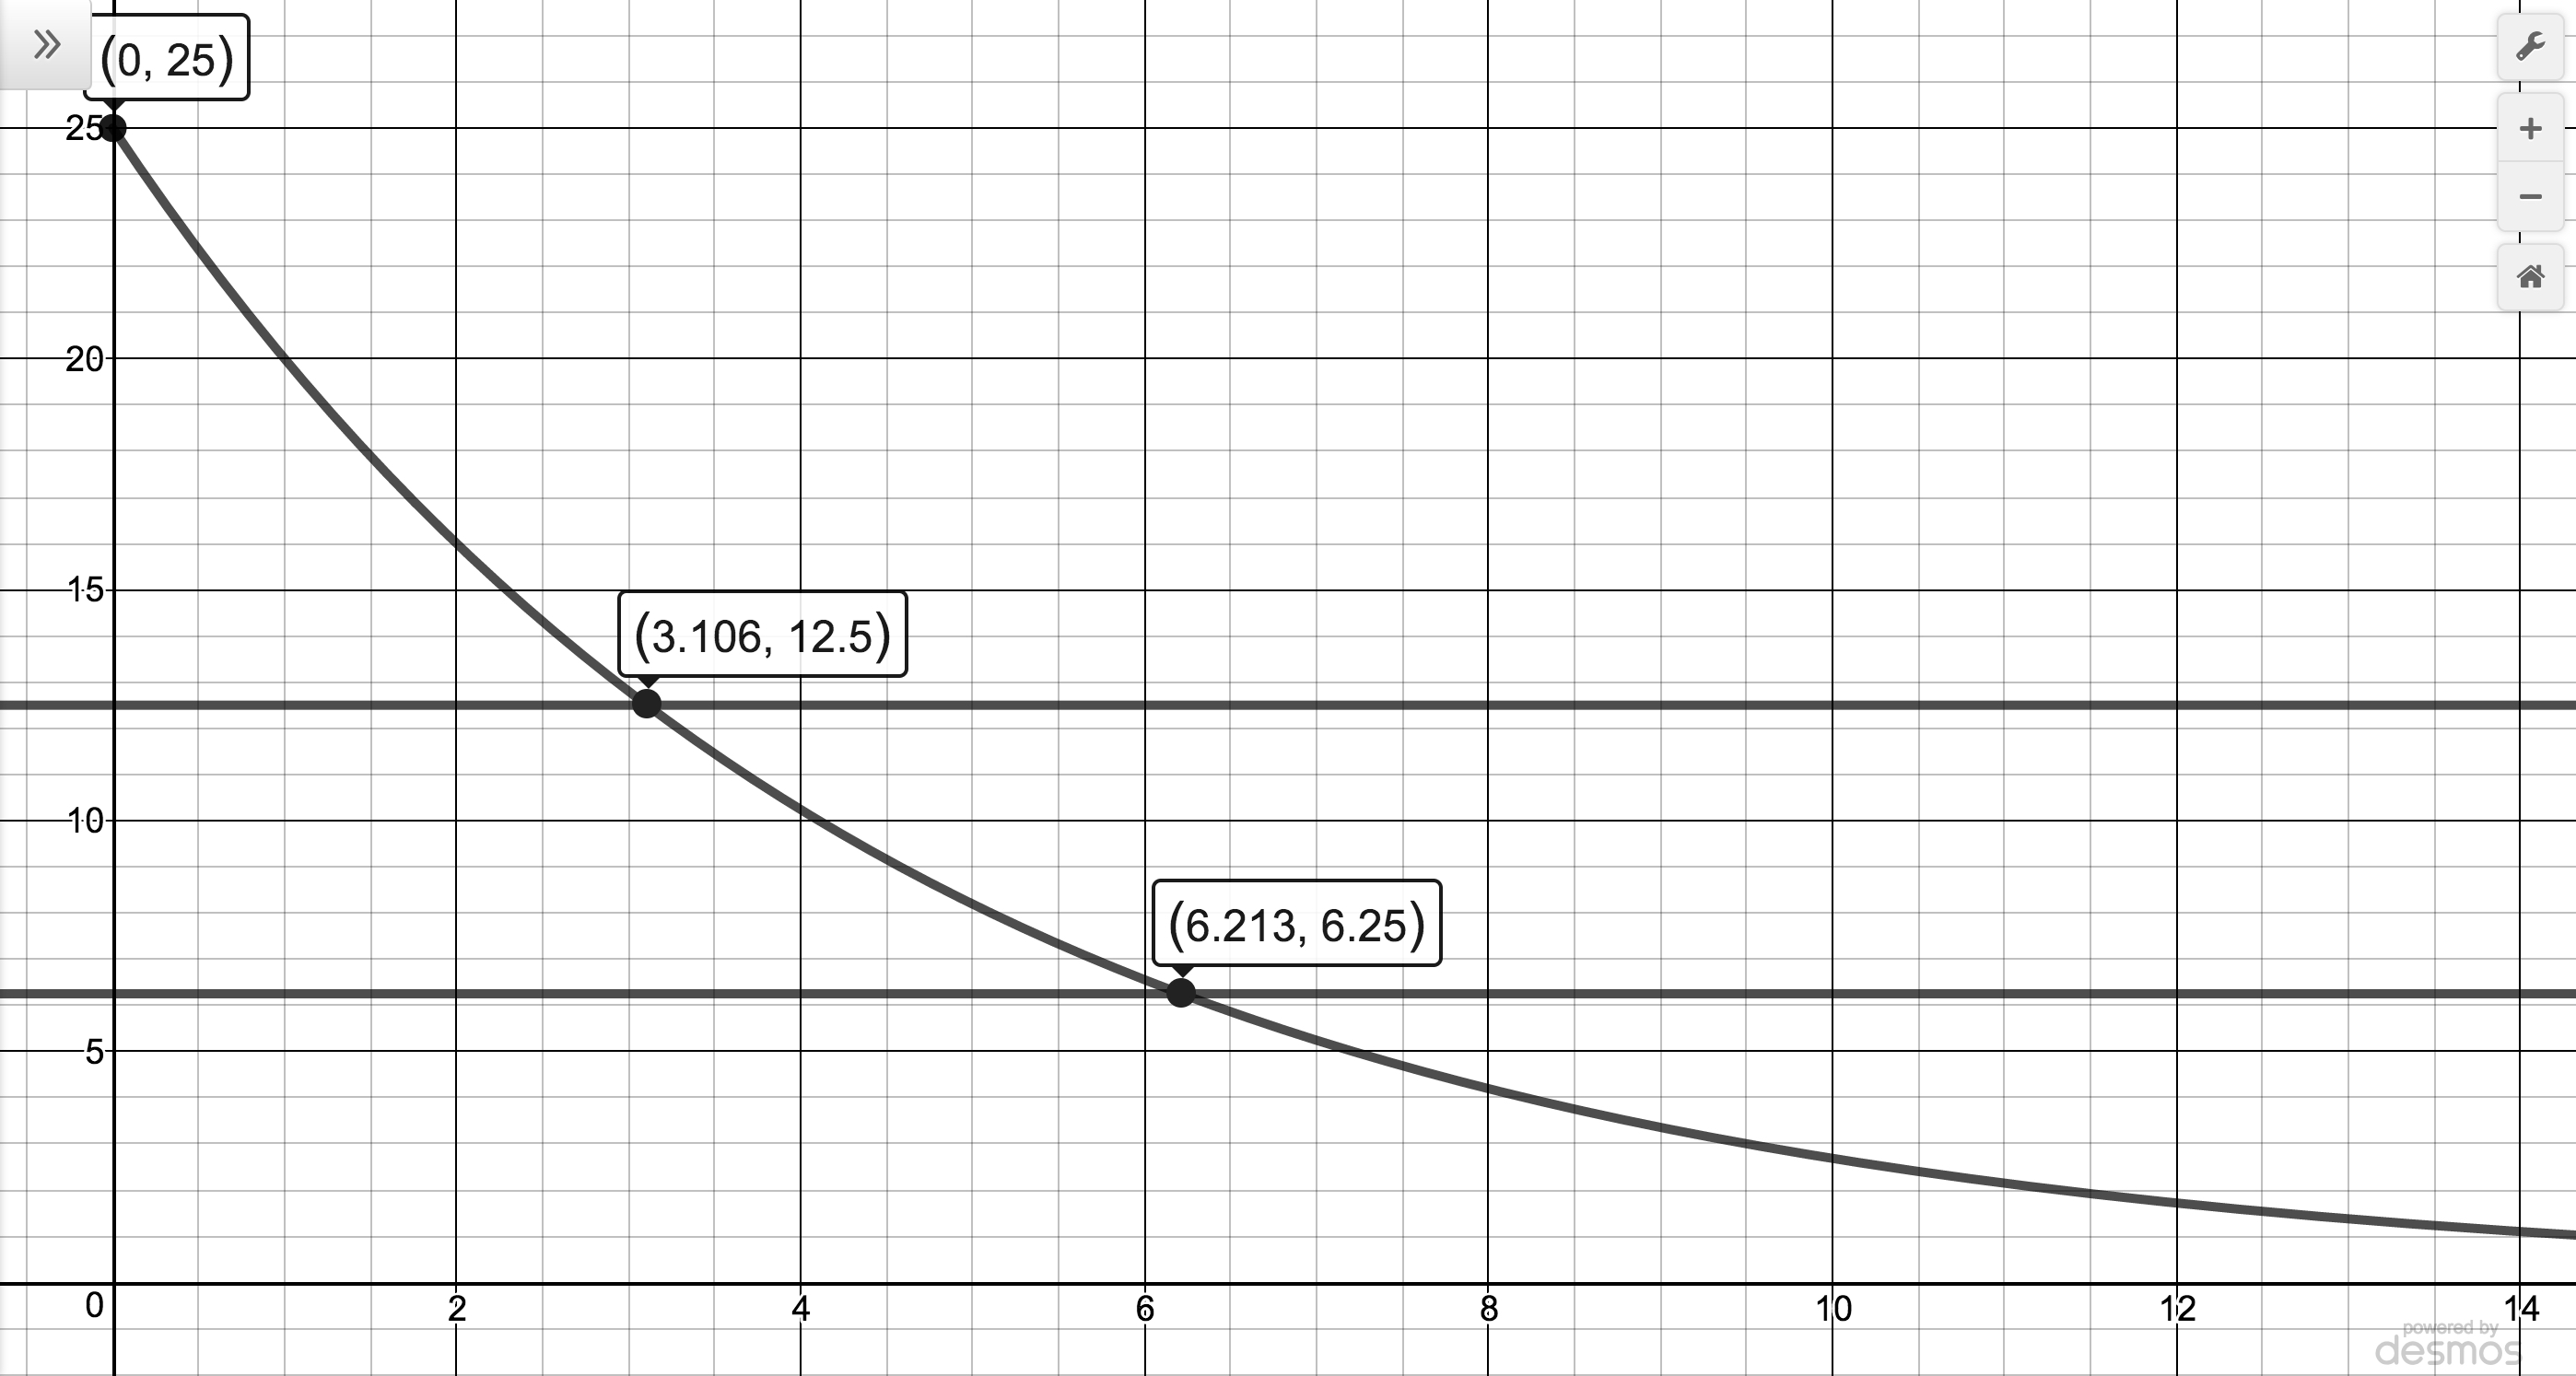
\includegraphics[width=6in]{./ExponentialFunctionsGraphics/ExponentialFunctionsEx01.jpg}

\end{center}

\qed
 
\end{enumerate}

\end{ex}

Some remarks about Example \ref{cardepreciationex} are in order.  First the function in the previous example is  called a `decay curve'.  Increasing exponential functions are used to model `growth curves' and we shall see several different examples of those in Section \ref{ExpLogApplications}.  

\smallskip

Second, as seen in numbers \ref{georatio1} and \ref{georatio2},  $V(t+1) = 0.8 V(t)$.  That is to say, the function $V$ has a \textit{constant unit multiplier}, in this case, $0.8$ because to obtain the function value $V(t+1)$, we \textit{multiply} the function value $V(t)$ by $b$.   It is not coincidence that the multiplier here is the base of the exponential, $0.8$.

\smallskip

Indeed, exponential functions of the form $f(x) = a \cdot b^{x}$  have a constant unit multiplier, $b$.  To see this,  note \[ \dfrac{f(x+1)}{f(x)} = \dfrac{a \cdot b^{x+1}}{ a \cdot b^{x}} = b^{1} = b.\]

Hence $f(x+1) = f(x) \cdot b$.  This will prove useful to us in Section \ref{ExpLogApplications} when making decisions about whether or not a data set represents exponential growth or decay.  

\smallskip

More generally, one can show (see Exercise \ref{exponentialchangeexercise}) for any real number $x_{0}$ that $f(x_{0}+\Delta x) = f(x_{0}) b^{\Delta x}$. That is, to obtain $f(x_{0} + \Delta x)$ from $f(x_{0})$, we \textit{multiply} by $\Delta x$ factors of the constant unit multiplier, $b$.  This is at the heart of what it means to be an exponential function.

\smallskip

If this discussion seems familiar, it should.  For linear functions, $f(x) = mx +b$, we can obtain the slope $m$ by computing $f(x+1) - f(x)$.  To see this, note $f(x+1) - f(x)  = (m(x+1) +b) - (mx+b) = m$ so that $f(x+1) = f(x) + m$.  In this way, we see that the slope $m$ is the constant unit \textit{addend} in that in order to obtain $f(x+1)$, we \textit{add} $m$ to the function value $f(x)$.  

\smallskip

This notion is solidified in the point-slope form of a linear function,  Equation \ref{linearfunctionpointslope}.  For for any real numbers $x$ and $x_{0}$, we have   $f(x) = f(x_{0}) + m(x-x_{0})$.  If we let $x = x_{0}+ \Delta x$, we get $f(x_{0}+ \Delta x) = f(x_{0}) + m \Delta x$.  In other words, to obtain $f(x_{0}+\Delta x)$ from $f(x_{0})$, we \textit{add} $m$ times $\Delta x$. 

\smallskip

Taking inspiration from linear functions, we define the `point-base' form of an exponential function below.

\smallskip

\colorbox{ResultColor}{\bbm

\begin{defn} \label{expfcnpointbaseform}  The \index{exponential function ! point-base form} \index{point-base form ! of an exponential function} \textbf{point-base form} of the exponential function $f(x) = a \cdot b^{x}$  is

\[ f(x) = f(x_{0}) b^{x - x_{0}} \]


\end{defn}

\ebm}

\smallskip

Just as the point-slope form of a linear function is helpful in building linear models, the point-base form of an exponential function will prove useful in building exponential models.

\smallskip

Next, while we saw in Example \ref{cardepreciationex} number \ref{cararcex}, exponential functions, unlike linear functions, do not have a constant rate of change.  However, in numbers \ref{carrelarcex1} and \ref{carrelarcex2}, we see that in some cases, they do have a constant \textit{relative} rate of change.  We define this notion below.

\smallskip


\colorbox{ResultColor}{\bbm

\begin{defn} \label{rrc}  Let $f$ be a function defined on the interval $[a,b]$ where $f(a) \neq 0$.

The \index{relative rate of change}\index{rate of change ! relative}\textbf{relative rate of  change}  of $f$ over $[a,b]$ is defined as: \[ \dfrac{\Delta [f(x)] }{f(a)} = \dfrac{f(b) - f(a)}{f(a)} .\]

\end{defn}

\ebm}

\smallskip

For exponential functions of the form $f(x) = a \cdot b^{x}$, we compute the relative rate of change over the interval $[x, x+1]$ and find it is constant:

\[ \dfrac{f(x+1) - f(x)}{f(x)} = \dfrac{f(x+1)}{f(x)} - \dfrac{f(x)}{f(x)} = b -1,\]

where we are using the fact that $\frac{f(x+1)}{f(x)} = b$. 

\smallskip

One way to interpret this result is when comparing $f(x)$ to $f(x+1)$, the exponential function grows (if $b>1$) or decays (if $b<1$) by $(b-1) \cdot 100 \%$.  In our example, $V(t) = 25 (0.8)^{t}$ so $b = 0.8$ and, as we saw, the relative rate of change from $V(t)$ to $V(t+1)$ was $ 0.8 - 1= -0.2$, meaning the value of the car  over the course of one year depreciates by  $20 \%$.

\smallskip

We close this section with another important application of exponential functions,  Newton's Law of Cooling.

\smallskip

\begin{ex}  \label{exptempex} According to \href{http://en.wikipedia.org/wiki/Heat_transfer#Newton.27s_law_of_cooling}{\underline{Newton's Law of Cooling}}\footnote{We will discuss this in greater detail in Section \ref{ExpLogApplications}.} the temperature of coffee $T(t)$ (in degrees Fahrenheit) $t$ minutes after it is served can be modeled by $T(t) = 70 + 90 e^{-0.1 t}$. \index{Newton's Law of Cooling}

\begin{enumerate}

\item  Find and interpret $T(0)$.

\item  Sketch the graph of $y = T(t)$ using transformations.

\item  Find and interpret the behavior of $T(t)$ as $ t \rightarrow \infty$.

\end{enumerate}

{\bf Solution.}

\begin{enumerate}

\item  Since $T(0) =70 + 90 e^{-0.1 (0)} = 160$,   the temperature of the coffee when it is served is $160^{\circ}\mbox{F}$.

\item  To graph $y = T(t)$ using transformations, we start with the basic function, $f(t)=e^{t}$.  As in Example \ref{expfcngraphsex}, we track the points $(-1, e^{-1}) \approx (-1, 0.368)$, $(0,1)$, and $(1, e) \approx (1, 2.718)$, along wth the horizontal asymptote $y = 0$ through each of transformations.

\smallskip

To use Theorem  \ref{transformationsthm}, we rewrite   $T(t) = 70 + 90e^{-0.1t} = 90e^{-0.1t}+70 = 90 f(-0.1t)+70$.   Following Theorem  \ref{transformationsthm}, we first  divide the $t$-coordinates of each point on the graph of $y=f(t)$ by $-0.1$ which results in a horizontal expansion by a factor of $10$ as well as a reflection about the $y$-axis.  

\smallskip

Next, we multiply the $y$-values of the points on this new graph by $90$ which effects a vertical stretch by a factor of $90$.  Last but not least, we  add $70$ to all of the $y$-coordinates of the points on this second graph, which shifts the graph upwards $70$ units.


\smallskip


Tracking points, we have $(-1, e^{-1})  \rightarrow (10, e^{-1}) \rightarrow (10, 90e^{-1}) \rightarrow (10, 90e^{-1}+70) \approx (10, 103.112)$, $(0,1) \rightarrow (0,1) \rightarrow (0,90) \rightarrow (0, 160)$, and $(1,e) \rightarrow (-10, e) \rightarrow (-10, 90e) \rightarrow (-10, 90e+70) \approx (-10, 314.62)$.  The horizontal asymptote $y=0$ is unaffected by the horizontal expansion, reflection about the $y$-axis, and the vertical stretch.  The vertical shift moves the horizontal asymptote up $70$ units, $y = 0 \rightarrow y = 70$. After restricting the domain to $t \geq 0$, we get the graph below on the right.

\[\begin{array}{ccc}

\begin{mfpic}[15]{-4}{4}{-1}{8}
\axes
\tlabel[cc](-1,1){\scriptsize $(0,1)$}
\tlabel[cc](0,-1.5){\scriptsize H.A. $y=0$}
\tlabel[cc](4,-0.5){\scriptsize $t$}
\tlabel[cc](0.5,8){\scriptsize $y$}
\tcaption{\scriptsize $y = f(t)=e^{t}$}
\ymarks{1,2,3,4,5,6,7}
\xmarks{-3,-2,-1,1,2,3}
\tlpointsep{4pt}
\axislabels {x}{{\scriptsize $-3 \hspace{7pt}$} -3, {\scriptsize $-2 \hspace{7pt}$} -2, {\scriptsize $-1 \hspace{7pt}$} -1, {\scriptsize $1$} 1, {\scriptsize $2$} 2, {\scriptsize $3$} 3}
\axislabels {y}{{\scriptsize $2$} 2,{\scriptsize $3$} 3,{\scriptsize $4$} 4,{\scriptsize $5$} 5,{\scriptsize $6$} 6,{\scriptsize $7$} 7}
\penwd{1.25pt}
\arrow \reverse \arrow \function{-3, 2, 0.1}{exp(x)}
\point[4pt]{(0,1),(1,2.718), (-1,0.368)}
\end{mfpic}

&

\stackrel{\xrightarrow{\hspace{1in}}}{\text{\scriptsize Theorem  \ref{transformationsthm}}} 

&

\begin{mfpic}[15]{-1}{11}{-1}{10}
\dashed \polyline{(-1,3.5),(11,3.5)}
\axes
\tlabel[cc](9,2.5){\scriptsize H.A. $y=70$}
\tlabel[cc](11,-0.5){\scriptsize $t$}
\tlabel[cc](0.5,10){\scriptsize $y$}
\tlabel[cc](-1, 8){\scriptsize $(0, 160)$}
\tcaption{\scriptsize $y = T(t)$}
\ymarks{1,2,3,4,5,6,7,8,9}
\xmarks{1,2,3,4,5,6,7,8,9,10}
\tlpointsep{4pt}
\axislabels {x}{{\scriptsize $2$} 1, {\scriptsize $4$} 2, {\scriptsize $6$} 3, {\scriptsize $8$} 4,{\scriptsize $10$} 5, {\scriptsize $12$} 6, {\scriptsize $14$} 7, {\scriptsize $16$} 8, {\scriptsize $18$} 9, {\scriptsize $20$} 10}
\axislabels {y}{{\scriptsize $20$} 1, {\scriptsize $40$} 2, {\scriptsize $60$} 3,{\scriptsize $80$} 4, {\scriptsize $100$} 5, {\scriptsize $120$} 6,{\scriptsize $140$} 7, {\scriptsize $180$} 9}
\penwd{1.25pt}
\arrow \function{0, 10, 0.1}{(90*exp(0-0.2*x)+70)/20}
\point[4pt]{(0,8),(5,5.15)}
\end{mfpic} \\

\end{array}\]

\item  We can determine the behavior of $T(t)$ as $t \rightarrow \infty$ two ways.  First, we can employ  the `number sense' developed in Chapter \ref{RationalFunctions}.    

\smallskip

That is, as $t \rightarrow \infty$, We get $T(t) = 70+90e^{-0.1t} \approx 70 +90e^{\mbox{\scriptsize very big $(-)$}}$.  Since $e > 1$, $e^{\mbox{\scriptsize very big $(-)$}}  \approx \mbox{very small $(+)$}$  The larger $t$ becomes, the smaller $e^{-0.1t}$ becomes, so the term $90 e^{-0.1t} \approx \mbox{very small $(+)$}$.  Hence, $T(t) = 70+90e^{-0.1t}  \approx 70 +  \mbox{very small $(+)$} \approx 70$. 

\smallskip

Alternatively, we can look to the graph of $y = T(t)$.  We know the horizontal asymptote is $y=70$ which means as $t \rightarrow \infty$, $T(t) \approx 70$.

\smallskip

In either case, we find that as time goes by,  the temperature of the coffee is cooling to $70^{\circ}$ Fahrenheit, ostensibly room temperature. \qed

\end{enumerate}

\end{ex}

\newpage

\subsection{Exercises}

\label{ExercisesforExponentialFunctions}

\label{IntroExpLogsExercises}

In Exercises \ref{graphexpfirsta} - \ref{graphexplasta}, sketch the graph of $g$ by starting with the graph of $f$ and using transformations.  Track at least three points of your choice and the horizontal asymptote through the transformations. State the domain and range of $g$.

\begin{multicols}{2}
\begin{enumerate}

\item  $f(x) = 2^{x}$, $g(x) = 2^{x} - 1$ \label{graphexpfirsta}

\item  $f(x) = \left(\frac{1}{3}\right)^{x}$, $g(x) = \left(\frac{1}{3}\right)^{x-1}$

\setcounter{HW}{\value{enumi}}
\end{enumerate}
\end{multicols}

\begin{multicols}{2}
\begin{enumerate}
\setcounter{enumi}{\value{HW}}

\item  $f(x) = 3^{x}$, $g(x) = 3^{-x}+2$

\item  $f(x) = 10^{x}$, $g(x) = 10^{\frac{x+1}{2}} - 20$  

\setcounter{HW}{\value{enumi}}
\end{enumerate}
\end{multicols}

\begin{multicols}{2}
\begin{enumerate}
\setcounter{enumi}{\value{HW}}

\item  $f(t) = (0.5)^{t}$, $g(t) = 100(0.5)^{0.1t}$

\item  $f(t) = (1.25)^{t}$, $g(t) = 1 - (1.25)^{t-2}$

\setcounter{HW}{\value{enumi}}
\end{enumerate}
\end{multicols}

\begin{multicols}{2}
\begin{enumerate}
\setcounter{enumi}{\value{HW}}

\item  $f(x) = e^{t}$, $g(x) = 8 - e^{-t}$

\item  $f(x) = e^{t}$, $g(x) = 10e^{-0.1t}$ \label{graphexplasta}

\setcounter{HW}{\value{enumi}}
\end{enumerate}
\end{multicols}

In Exercises, \ref{expformfirsta} - \ref{expformlasta}, the graph of an exponential function is given.  Find a formula for the function in the form $F(x) = a \cdot 2^{bx-h}+k$.

\begin{multicols}{2}
\begin{enumerate}
\setcounter{enumi}{\value{HW}}

\item  \label{expformfirsta}  Points:  $\left(-2, -\frac{5}{2} \right)$,  $\left(-1, -2 \right)$, $\left(0, -1 \right)$, \\
Asymptote:  $y = -3$. \\

\begin{mfpic}[13]{-5}{3}{-4}{6}
\axes
\tlabel[cc](3,-0.5){\scriptsize $x$}
\tlabel[cc](0.5,6){\scriptsize $y$}
\xmarks{-4, -3,-2,-1,1,2}
\ymarks{-3, -2, -1, 1,2,3,4,5}
\tlpointsep{4pt}
\axislabels {x}{{\scriptsize $-4 \hspace{7pt}$} -4,{\scriptsize $-3 \hspace{7pt}$} -3, {\scriptsize $-2 \hspace{7pt}$} -2, {\scriptsize $-1 \hspace{7pt}$} -1, {\scriptsize $1$} 1, {\scriptsize $2$} 2}
\axislabels {y}{{\scriptsize $1$} 1, {\scriptsize $2$} 2, {\scriptsize $3$} 3, {\scriptsize $4$} 4, {\scriptsize $5$} 5, {\scriptsize $-1$} -1, {\scriptsize $-2$} -2, {\scriptsize $-3$} -3}
\dashed \polyline{(-5,-3), (3,-3)}
\penwd{1.25pt}
\arrow \reverse \arrow \function{-4.5, 2.1, 0.1}{(2**(x+1))-3}
\point[4pt]{(-2, -2.5), (-1,-2),(0,-1)}
\end{mfpic}

\vfill

\columnbreak

\item  Points:  $\left(-1, 1 \right)$, $\left(0, 2 \right)$, $\left(1, \frac{5}{2} \right)$, \\
Asymptote:  $y = 3$. \\

\begin{mfpic}[13]{-4}{4}{-6}{4}
\axes
\tlabel[cc](4,-0.5){\scriptsize $x$}
\tlabel[cc](0.5,4){\scriptsize $y$}
\xmarks{-3,-2,-1,1,2,3}
\ymarks{-5 step 1 until 3}
\tlpointsep{4pt}
\axislabels {x}{{\scriptsize $-3 \hspace{7pt}$} -3, {\scriptsize $-2 \hspace{7pt}$} -2, {\scriptsize $-1 \hspace{7pt}$} -1, {\scriptsize $1$} 1, {\scriptsize $2$} 2, {\scriptsize $3$} 3}
\axislabels {y}{{\scriptsize $1$} 1, {\scriptsize $2$} 2, {\scriptsize $3$} 3, {\scriptsize $-1$} -1, {\scriptsize $-2$} -2, {\scriptsize $-3$} -3, {\scriptsize $-4$} -4, {\scriptsize $-5$} -5}
\dashed \polyline{(-4,3), (4,3)}
\penwd{1.25pt}
\arrow \reverse \arrow \function{-3, 3.1, 0.1}{3-(2**(-x))}
\point[4pt]{(-1,1), (0,2), (1, 2.5)}
\end{mfpic}



\setcounter{HW}{\value{enumi}}
\end{enumerate}
\end{multicols}

\begin{multicols}{2}
\begin{enumerate}
\setcounter{enumi}{\value{HW}}

\item  Points:  $\left(\frac{5}{2}, \frac{1}{2} \right)$, $\left(3,1 \right)$, $\left(\frac{7}{2}, 2 \right)$, \\
Asymptote:  $y = 0$. \\

\begin{mfpic}[13]{-1}{5}{-1}{9}
\axes
\tlabel[cc](5,-0.5){\scriptsize $x$}
\tlabel[cc](0.5,9){\scriptsize $y$}
\xmarks{1 step 1 until 4}
\ymarks{1 step 1 until 8}
\tlpointsep{4pt}
\axislabels {x}{{\scriptsize $1$} 1, {\scriptsize $2$} 2, {\scriptsize $3$} 3, {\scriptsize $4$} 4}
\axislabels {y}{{\scriptsize $1$} 1, {\scriptsize $2$} 2, {\scriptsize $3$} 3, {\scriptsize $4$} 4, {\scriptsize $5$} 5, {\scriptsize $6$} 6, {\scriptsize $7$} 7, {\scriptsize $8$} 8}
\penwd{1.25pt}
\arrow \reverse \arrow \function{1.25, 4.55, 0.1}{2**(2*x-6)}
\point[4pt]{(2.5, 0.5), (3,1), (3.5,2) }
\end{mfpic}

\vfill

\columnbreak

\item  Points:  $\left(-\frac{1}{2}, 6 \right)$, $\left(0,3 \right)$, $\left(\frac{1}{2}, \frac{3}{2} \right)$, \\
Asymptote:  $y = 0$.   \\

\begin{mfpic}[13]{-4}{4}{-1}{9}
\axes
\tlabel[cc](4,-0.5){\scriptsize $x$}
\tlabel[cc](0.5,9){\scriptsize $y$}
\xmarks{-3,-2,-1,1,2,3}
\ymarks{1,2,3,4,5,6,7,8}
\tlpointsep{4pt}
\axislabels {x}{{\scriptsize $-3 \hspace{7pt}$} -3, {\scriptsize $-2 \hspace{7pt}$} -2, {\scriptsize $-1 \hspace{7pt}$} -1, {\scriptsize $1$} 1, {\scriptsize $2$} 2, {\scriptsize $3$} 3}
\axislabels {y}{{\scriptsize $1$} 1, {\scriptsize $2$} 2, {\scriptsize $3$} 3,  {\scriptsize $7$} 7, {\scriptsize $8$} 8}
\penwd{1.25pt}
\arrow \reverse \arrow \function{-0.79, 2, 0.1}{3*(2**(-2*x))}
\point[4pt]{(-0.5, 6), (0,3), (0.5, 1.5)}
\end{mfpic}


\label{expformlasta} 

\setcounter{HW}{\value{enumi}}
\end{enumerate}
\end{multicols}


\begin{enumerate}
\setcounter{enumi}{\value{HW}}


\item 

Find a formula for each graph in Exercises \ref{expformfirsta} - \ref{expformlasta} of the form $G(x) = a \cdot 4^{bx-h} + k$.
  Did you change your solution methodology?    What is the relationship between your answers for $F(x)$ and $G(x)$ for each graph?

\item \label{morethanoneforexpexercise} In Example \ref{expfcngraphsex} number \ref{findformulaforexpexample}, we obtained the solution  $F(x) = -2^{x+3} + 4$ as one formula for the given graph by making a simplifying assumption that $a = -1$.  This exercises explores if there are any other solutions for different choices of $a$.

\begin{enumerate}

\item  Show  $G(x) = -4 \cdot 2^{x+1} + 4$ also fits the data for the given graph, and use  properties of exponents to show $G(x) = F(x)$.  (Use the fact that $4 = 2^2$ \ldots)

\item With help from your classmates, find solutions to  Example \ref{expfcngraphsex} number \ref{findformulaforexpexample} using $a = -8$, $a = -16$ and  $a = -\frac{1}{2}$.  Show all your solutions can be rewritten as: $F(x) = -2^{x+3} + 4$.

\item  Using properties of exponents and the fact that the range of $2^{x}$ is $(0, \infty)$, show that any function of the form $f(x) = -a \cdot 2^{bx-h} + k$ for $a> 0$ can be rewritten as $f(x) = - 2^{c} \, 2^{bx-h} + k = -2^{bx-h+c} + k$.  Relabeling, this means every function of the form $f(x) = -a \cdot 2^{bx-h} + k$ with four parameters ($a$, $b$, $h$, and $k$) can be rewritten as $f(x) =  - 2^{bx - H} + k$, a formula with just three parameters:  $b$, $H$, and $k$.  Conclude that  \textit{every} solution to Example \ref{expfcngraphsex} number \ref{findformulaforexpexample} reduces to $F(x) = -2^{x+3} + 4$ .

\end{enumerate}
\setcounter{HW}{\value{enumi}}
\end{enumerate}

In Exercises \ref{decomposebasicexpfirst} - \ref{decomposebasicexplast}, write the given function as a nontrivial decomposition of functions as directed.

\begin{enumerate}
\setcounter{enumi}{\value{HW}}

\item  For $f(x) = e^{-x} +1 $, find functions $g$ and $h$ so that $f=g+h$. \label{decomposebasicexpfirst}
\item  For $f(x) = e^{2x} - x$, find functions $g$ and $h$ so that $f=g-h$. 
\item  For $f(t) = t^2 e^{-t}$, find functions $g$ and $h$ so that $f=gh$.
\item  For $r(x) = \dfrac{e^{x} - e^{-x}}{e^{x}+e^{-x}}$, find functions $f$ and $g$ so $r = \dfrac{f}{g}$.
\item  For $k(x) = e^{-x^2}$, find functions $f$ and $g$  so that $k = g \circ f$.
\item  For $s(x) =\sqrt{e^{2x} - 1}$, find functions $f$ and $g$ so $s = g \circ f$. \label{decomposebasicexplast}


\item \label{preludetocompoundingexercise} The amount of money in a savings account, $A(t)$, in dollars,  $t$ years after an initial investment is made is given by: $A(t) = 500(1.05)^{t}$, for $t \geq 0$.

\begin{enumerate}

\item  Find and interpret $A(0)$, $A(1)$, and $A(2)$.  

\item  Find and interpret the relative rate of change of $A$ over the intervals $[0,1]$, $[1,2]$, $[0,2]$.

\item  Find, simplify, and interpret the relative rate of change of $A$ over the $[t, t+1]$.  Assume  $t \geq 0$.

\item Use a graphing utility to estimate how long until the savings account is worth $\$1500$.  Round your answer to the nearest year.

\end{enumerate}

\pagebreak

\item  Based on census data,\footnote{See \href{http://www.towncharts.com/Ohio/Demographics/Lake-County-OH-Demographics-data.html}{\underline{here}}.} the population of Lake County, Ohio, in 2010 was 230,041 and in 2015, the population was 229,437.  

\begin{enumerate}

\item  Show the percentage change in the population from 2010 to 2015 is approximately $-0.263 \%$.

\item  If this percentage change remains constant, predict the population of Lake County in 2020.

\item  \label{populationfiveyear} Assuming this percentage change per five years remains constant, find an expression for the population $P(t)$ of Lake County where $t$ is the number of five year intervals after 2010.  (So $t = 0$ corresponds to 2010, $t = 1$ corresponds to $2015$, $t = 2$ corresponds to $2020$, etc.)

HINT:  Definitions \ref{expfcnpointbaseform} and \ref{rrc} and ensuing discussion on that page is useful here.

\item  Use your answer to  \ref{populationfiveyear}  to predict the population of Lake County in the year 2017.  

\item  Let $A(t)$  represent the population of Lake County $t$ years after 2010 where the we approximate the percentage change in population per year as $-\frac{0.263 \%}{5} = -0.0526 \%$.    Find a formula for $A(t)$ and compare your predictions with $A(t)$ to those given by $P(t)$.  In particular, what population does each model give for the year 2050?  Discuss any discrepancies with your classmates.

\end{enumerate}


\item \label{averageofarc}  Show that the average rate of change of a function over the interval  $[x, x+2]$ is average of the average rates of change of the function over the intervals $[x,x+1]$ and $[x+1, x+2]$.  Can the same be said for the average rate of change of the function over $[x, x+3]$ and the average of the average rates of change over $[x, x+1]$, $[x+1, x+2]$, and $[x+2, x+3]$?  Generalize.

\item \label{exponentialchangeexercise}  If $f(x) = b^{x}$ where $b>0$, $b \neq 1$,  show $f(x_{0}+\Delta x) = f(x_{0}) b^{\Delta x}$.


\item Which is larger: $e^{\pi}$ or $\pi^{e}$?  How do you know?  Can you find a proof that doesn't use technology?

\setcounter{HW}{\value{enumi}}
\end{enumerate}


\newpage

\subsection{Answers}

\begin{multicols}{2}
\begin{enumerate}


\item  Domain of $g$:  $(-\infty, \infty)$\\
 Range of $g$:  $(-1, \infty)$\\
 Points:  $\left(-1, -\frac{1}{2} \right)$, $(0,0)$, $(1,1)$\\
Asymptote: $y = -1$\\
 
\begin{mfpic}[15]{-4}{4}{-2}{9}
\point[4pt]{(-1,-0.5), (0,0), (1,1)}
\axes
\tlabel[cc](4,-0.5){\scriptsize $x$}
\tlabel[cc](0.5,9){\scriptsize $y$}
\tcaption{$y = g(x) = 2^{x}-1$}
\xmarks{-3,-2,-1,1,2,3}
\ymarks{-1,1,2,3,4,5,6,7,8}
\tlabel[cc](-3,0.5){\tiny $-3 \hspace{7pt}$}
\tlabel[cc](-2,0.5){\tiny $-2 \hspace{7pt}$}
\tlabel[cc](-1,0.5){\tiny $-1 \hspace{7pt}$}
\tlpointsep{4pt}
\axislabels {x}{{\tiny $1$} 1, {\tiny $2$} 2, {\tiny $3$} 3}
\axislabels {y}{{\tiny $1$} 1, {\tiny $2$} 2, {\tiny $3$} 3, {\tiny $4$} 4, {\tiny $5$} 5, {\tiny $6$} 6, {\tiny $7$} 7, {\tiny $8$} 8}
\dashed \polyline{(-4,-1),(4,-1)}
\penwd{1.25pt}
\arrow \reverse \arrow \function{-3.5, 3.1, 0.1}{(2**(x))-1}
\end{mfpic}

\vfill

\columnbreak

\item  Domain of $g$:  $(-\infty, \infty)$ \\
 Range of $g$:  $(0, \infty)$ \\
  Points:  $(0,3)$, $(1,1)$, $\left(2, \frac{1}{3} \right)$\\
 Asymptote: $y = 0$\\
 
\begin{mfpic}[15]{-4}{4}{-1}{10}
\point[4pt]{(0,3), (1,1), (2,0.3333)}
\axes
\tlabel[cc](4,-0.5){\scriptsize $x$}
\tlabel[cc](0.5,10){\scriptsize $y$}
\tcaption{$y = g(x) = \left(\frac{1}{3}\right)^{x-1}$}
\xmarks{-3,-2,-1,1,2,3}
\ymarks{1,2,3,4,5,6,7,8,9}
\tlpointsep{4pt}
\axislabels {x}{{\tiny $-3 \hspace{7pt}$} -3, {\tiny $-2 \hspace{7pt}$} -2, {\tiny $-1 \hspace{7pt}$} -1, {\tiny $1$} 1, {\tiny $2$} 2, {\tiny $3$} 3}
\axislabels {y}{{\tiny $1$} 1, {\tiny $2$} 2, {\tiny $3$} 3, {\tiny $4$} 4, {\tiny $5$} 5, {\tiny $6$} 6, {\tiny $7$} 7, {\tiny $8$} 8, {\tiny $9$} 9}
\penwd{1.25pt}
\arrow \reverse \arrow \function{-1.05, 3.5, 0.1}{3**(1-x)}
\end{mfpic} 

\setcounter{HW}{\value{enumi}}
\end{enumerate}
\end{multicols}

\begin{multicols}{2}
\begin{enumerate}
\setcounter{enumi}{\value{HW}}

\item  Domain of $g$:  $(-\infty, \infty)$\\
 Range of $g$:  $(2, \infty)$\\
  Points:  $\left(1, \frac{7}{3} \right)$, $(0,3)$, $(-1,5)$\\
  Asymptote:  $y = 2$ \\

\begin{mfpic}[15]{-4}{4}{-1}{12}
\point[4pt]{(1,2.3333), (0,3), (-1,5)}
\axes
\tlabel[cc](4,-0.5){\scriptsize $x$}
\tlabel[cc](0.5,12){\scriptsize $y$}
\tcaption{$y = g(x) = 3^{-x}+2$}
\xmarks{-3,-2,-1,1,2,3}
\ymarks{1,2,3,4,5,6,7,8,9,10,11}
\tlpointsep{4pt}
\axislabels {x}{{\tiny $-3 \hspace{7pt}$} -3, {\tiny $-2 \hspace{7pt}$} -2, {\tiny $-1 \hspace{7pt}$} -1, {\tiny $1$} 1, {\tiny $2$} 2, {\tiny $3$} 3}
\axislabels {y}{{\tiny $1$} 1, {\tiny $2$} 2, {\tiny $3$} 3, {\tiny $4$} 4, {\tiny $5$} 5, {\tiny $6$} 6, {\tiny $7$} 7, {\tiny $8$} 8, {\tiny $9$} 9, {\tiny $10$} 10, {\tiny $11$} 11}
\dashed \polyline{(-4,2),(4,2)}
\penwd{1.25pt}
\arrow \reverse \arrow \function{-2.05, 2.5, 0.1}{2+3**(0-x)}
\end{mfpic}

\vfill

\columnbreak

\item  Domain of $g$:  $(-\infty, \infty)$\\
 Range of $g$:  $(-20, \infty)$\\
  Points:  $\left(-1,-19 \right)$, $(1,-10)$, $(3,80)$\\
  Asymptote:  $y = -20$\\
 
\begin{mfpic}[15]{-3}{4}{-2}{9}
\point[4pt]{(-1,-1.9), (1,-1), (3,8)}
\axes
\tlabel[cc](4,-0.5){\scriptsize $x$}
\tlabel[cc](0.5,9){\scriptsize $y$}
\tcaption{$y = g(x) = 10^{\frac{x+1}{2}}-20$}
\xmarks{-3,-2,-1,1,2,3}
\ymarks{-2,-1,1,2,3,4,5,6,7,8}
\tlpointsep{4pt}
\axislabels {x}{{\tiny $-3 \hspace{7pt}$} -3, {\tiny $-2 \hspace{7pt}$} -2,  {\tiny $1$} 1, {\tiny $2$} 2, {\tiny $3$} 3}
\axislabels {y}{{\tiny $-10$} -1,{\tiny $10$} 1, {\tiny $20$} 2, {\tiny $30$} 3, {\tiny $40$} 4, {\tiny $50$} 5, {\tiny $60$} 6, {\tiny $70$} 7, {\tiny $80$} 8}
\dashed \polyline{(-4,-2), (4,-2)}
\penwd{1.25pt}
\arrow \reverse \arrow \function{-3, 3.06, 0.1}{((10**((x+1)/2))-20)/10}
\end{mfpic}

\setcounter{HW}{\value{enumi}}
\end{enumerate}
\end{multicols}

\begin{multicols}{2}
\begin{enumerate}
\setcounter{enumi}{\value{HW}}

\item  Domain of $g$:  $(-\infty, \infty)$\\
  Range of $g$:  $(0, \infty)$ \\
  Points:  $(-10, 200)$, $(0, 100)$, $(10, 50)$\\
  Asymptote: $y = 0$\\
 
\begin{mfpic}[15]{-4}{4}{-1}{9}
\point[4pt]{(-1,2), (0,1), (1, 0.5)}
\axes
\tlabel[cc](4,-0.5){\scriptsize $t$}
\tlabel[cc](0.5,9){\scriptsize $y$}
\tcaption{ $y = g(t) = 100(0.5)^{0.1t}$}
\xmarks{-3,-2,-1,1,2,3}
\ymarks{1,2,3,4,5,6,7,8}
\tlpointsep{4pt}
\axislabels {x}{{\tiny $-30 \hspace{7pt}$} -3, {\tiny $-20 \hspace{7pt}$} -2, {\tiny $-10 \hspace{7pt}$} -1, {\tiny $10$} 1, {\tiny $20$} 2, {\tiny $30$} 3}
\axislabels {y}{{\tiny $100$} 1, {\tiny $200$} 2, {\tiny $300$} 3, {\tiny $400$} 4, {\tiny $500$} 5, {\tiny $600$} 6, {\tiny $700$} 7, {\tiny $800$} 8}
\penwd{1.25pt}
\arrow \reverse \arrow \function{-3, 3, 0.1}{0.5**x}
\end{mfpic}

\vfill

\columnbreak


\item  Domain of $g$:  $(-\infty, \infty)$\\
  Range of $g$:  $(-\infty, 1)$ \\
  Points:  $(1, 0.2)$, $(2,0)$, $(3,-0.25)$\\
  Asymptote: $y = 1$\\
 
\begin{mfpic}[10][8]{-8}{5}{-11}{11}
\point[4pt]{(1,2), (2,0), (3, -2.5)}
\axes
\tlabel[cc](5,-0.5){\scriptsize $t$}
\tlabel[cc](0.5,11){\scriptsize $y$}
\tcaption{ $y = g(t) = 1-(1.25)^{t-2}$}
\xmarks{-8 step 1 until 4}
\ymarks{-10 step 1 until 10}
\tlpointsep{4pt}
\axislabels {x}{{\tiny $-8 \hspace{7pt}$} -8,{\tiny $-6 \hspace{7pt}$} -6,{\tiny $-4 \hspace{7pt}$} -4,{\tiny $-2 \hspace{7pt}$} -2, {\tiny $2$} 2, {\tiny $4$} 4}
\axislabels {y}{ {\tiny $0.2$} 2,  {\tiny $0.4$} 4,  {\tiny $0.6$} 6, {\tiny $0.8$} 8, {\tiny $1$} 10, {\tiny $-0.2$} -2, {\tiny $-0.4$} -4,  {\tiny $-0.6$} -6, {\tiny $-0.8$} -8, {\tiny $-1$} -10}
 
\dashed \polyline{(-8, 10), (5, 10)}
\penwd{1.25pt}
\arrow \reverse \arrow \function{-8, 5, 0.1}{(1- (1.25**(x-2)))*10}
\end{mfpic}

\setcounter{HW}{\value{enumi}}
\end{enumerate}
\end{multicols}



\begin{multicols}{2}
\begin{enumerate}
\setcounter{enumi}{\value{HW}}

\item  Domain of $g$:  $(-\infty, \infty)$\\
 Range of $g$:  $(-\infty, 8)$ \\
  Points:  $\left(1, 8-e^{-1} \right) \approx (1, 7.63)$,  \\
  $(0,7)$, $\left(-1,  8-e \right) \approx (1,5.28) $\\
 Asymptote:  $y = 8$ \\
 
\begin{mfpic}[15]{-4}{4}{-1}{9}
\point[4pt]{(1,7.6321), (0,7), (-1,5.282)}
\axes
\tlabel[cc](4,-0.5){\scriptsize $t$}
\tlabel[cc](0.5,9){\scriptsize $y$}
\tcaption{ $y = g(t) = 8-e^{-t}$}
\xmarks{-3,-2,-1,1,2,3}
\ymarks{1,2,3,4,5,6,7,8}
\tlpointsep{4pt}
\axislabels {x}{{\tiny $-3 \hspace{7pt}$} -3, {\tiny $-2 \hspace{7pt}$} -2, {\tiny $-1 \hspace{7pt}$} -1, {\tiny $1$} 1, {\tiny $2$} 2, {\tiny $3$} 3}
\axislabels {y}{{\tiny $1$} 1, {\tiny $2$} 2, {\tiny $3$} 3, {\tiny $4$} 4, {\tiny $5$} 5, {\tiny $6$} 6, {\tiny $7$} 7, {\tiny $8$} 8}
\dashed \polyline{(-4,8), (4,8)}
\penwd{1.25pt}
\arrow \reverse \arrow \function{-2.25, 2, 0.1}{8-exp(0-x)}
\end{mfpic}

\vfill

\columnbreak


\item  Domain of $g$:  $(-\infty, \infty)$\\
 Range of $g$:  $(0, \infty)$\\
 Points:  $\left(10, 10e^{-1} \right) \approx (10, 3.68)$ \\
 $(0,10)$, $\left(-10, 10e \right) \approx (-10, 27.18)$  \\
 Asymptote:  $y = 0$\\
 
\begin{mfpic}[15]{-4}{4}{-1}{9}
\point[4pt]{(1,0.3679), (0,1), (-1,2.718)}
\axes
\tlabel[cc](4,-0.5){\scriptsize $t$}
\tlabel[cc](0.5,9){\scriptsize $y$}
\tcaption{$y = g(t) = 10e^{-0.1t}$}
\xmarks{-3,-2,-1,1,2,3}
\ymarks{1,2,3,4,5,6,7,8}
\tlpointsep{4pt}
\axislabels {x}{{\tiny $-10 \hspace{7pt}$} -1, {\tiny $10$} 1, {\tiny $20$} 2, {\tiny $30$} 3}
\axislabels {y}{{\tiny $10$} 1, {\tiny $20$} 2, {\tiny $30$} 3, {\tiny $40$} 4, {\tiny $50$} 5, {\tiny $60$} 6, {\tiny $70$} 7, {\tiny $80$} 8}
\penwd{1.25pt}
\arrow \reverse \arrow \function{-2.15, 2, 0.1}{exp(0-x)}
\end{mfpic}

\setcounter{HW}{\value{enumi}}
\end{enumerate}
\end{multicols}

\begin{multicols}{4}
\begin{enumerate}
\setcounter{enumi}{\value{HW}}

\item $F(x) = 2^{x+1}-3$

\item  $F(x) = -2^{-x} + 3$

\item $F(x) = 2^{2x-6}$

\item  $F(x) =3 \cdot 2^{-2x}$

\setcounter{HW}{\value{enumi}}
\end{enumerate}
\end{multicols}

\begin{enumerate}
\setcounter{enumi}{\value{HW}}

\item  Since $2 = 4^{\frac{1}{2}}$, one way to obtain the formulas for $G(x)$ is to use properties of exponents.  For example, $F(x) = 2^{x+1}-3 = \left(4^{\frac{1}{2}}\right)^{x+1} -3 = 4^{\frac{1}{2}(x+1)} - 3 = 4^{\frac{1}{2} x + \frac{1}{2}} - 3$.  In order, the formulas for $G(x)$ are:

\begin{multicols}{4}
\begin{itemize}

\item $G(x) = 4^{\frac{1}{2}x+\frac{1}{2}}-3$

\item  $G(x) = -4^{-\frac{1}{2} x} + 3$

\item $G(x) = 4^{x-3}$

\item  $G(x) =3 \cdot 4^{-x}$

\end{itemize}
\end{multicols}

\addtocounter{enumi}{1}

\item  One solution is $g(x)  = e^{-x}$ and $h(x) = 1$.
\item  One solution is $g(x) = e^{2x}$ and $h(x) = x$.
\item  One solution is $g(t) = t^2$ and $h(t) = e^{-t}$.
\item  One solution is $f(x) = e^{x} - e^{-x}$ and $g(x) = e^{x}+e^{-x}$.
\item  One solution is $f(x) = -x^2$ and $g(x) = e^{x}$.
\item  One solution is $f(x) = e^{2x} -1$ and $g(x) = \sqrt{x}$.  


\item  \begin{enumerate}

\item   $A(0) = 500$, so the initial balance in the savings account is $\$500$.  $A(1) = 525$, so after $1$ year, there is $\$525$ in the savings account.   $A(2) =551.25$, so after $2$ years, there is $\$551.25$ in the savings account. 

\item  The relative rate of change of $A$ over the intervals $[0,1]$ and $[1,2]$ is $0.05$ which means the savings account is growing by $5 \%$ each year for those two years.  Over the interval $[0,2]$, the relative rate of change is $0.1025$ meaning the account has grown by $10.25 \%$ over the course of the first two years.  Note this is greater than the sum of the two rates $5 \% + 5 \% = 10 \%$.  This is due to the `compounding effect' and will be discussed in greater detail in Section \ref{ExpLogApplications}.

\item  The relative rate of change of $A$ over the $[t, t+1]$ is $0.05$. This means over the course of one year, the savings account grows by $5 \%$.

\item Graphing $y= A(t)$ and $y = 1500$, we find they intersect when $t \approx 22.5$ so it takes approximately $22-23$ years for the savings account to grow to $\$1500$ in value.

\end{enumerate}

\item  \begin{enumerate}

\item $\dfrac{229437-230041}{230041} \approx 0.263 \%$.

\item  Since 2020 is five years after 2015, we expect the population to decrease by  $0.263 \%$ of 229437, or approximately 603 people.  Hence, we approximate the population in 2020 as 228834.

\item  $P(t) = 230041(1-0.00263)^t = 230041(0.99737)^{t}$, $t \geq 0$.

\item  Since 2017 is 7 years after 2010, we set $t = \frac{7}{5} = 1.4$ and find $P(1.4) \approx 229194$.  So the population is approximately 229, 194 in 2017.  

\item  $A(t) = 230041(1 - 0.0005626)^{t} =  230041 (0.999474)^{t}$, $t \geq 0$.  Since 2050 is 40 years after 2010, using the model $P(t)$, we divide $\frac{40}{5} = 8$ and find $P(8) \approx 225,245$. On the other hand, $A(40) \approx 225,250$.  This is more than roundoff error.  There is a compounding effect which makes the functions $A(t)$ and $P(t)$ different. \footnote{See number \ref{preludetocompoundingexercise} above or, for more, see Section \ref{ExpLogApplications}.}

\end{enumerate}


\setcounter{HW}{\value{enumi}}
\end{enumerate}




\closegraphsfile

\newpage

\section{Logarithmic Functions}

\mfpicnumber{1}

\opengraphsfile{LogarithmicFunctions}

\setcounter{footnote}{0}

\label{LogarithmicFunctions}


In Section \ref{ExponentialFunctions}, we saw exponential functions $f(x) = b^x$  are are one-to-one which means they are invertible.   In this section, we explore their inverses, the \textit{logarithmic functions} which are called `logs' for short.

\smallskip

\colorbox{ResultColor}{\bbm

\begin{defn} \label{logfcndefn} For the exponential function $f(x) = b^{x}$,  $f^{-1}(x) = \log_{b}(x)$ is called the \index{function ! logarithmic} \textbf{base \boldmath $b$ logarithm function}.  We read `$\log_{b}(x)$' as `log base $b$ of $x$.' \index{logarithm ! general, ``base $b$''}

\end{defn}

\ebm}
\smallskip

We have special notations for the common base, $b=10$, and the natural base, $b=e$.


\smallskip

\colorbox{ResultColor}{\bbm

\begin{defn} $~$

\begin{itemize}

\item  The \index{logarithm ! common} \textbf{common logarithm} of a real number $x$ is $\log_{10}(x)$ and is usually written $\log(x)$.   

\item The \index{logarithm ! natural} \textbf{natural logarithm} of a real number $x$ is $\log_{e}(x)$ and is usually written $\ln(x)$. \index{common logarithm} \index{natural logarithm}

\end{itemize}

\end{defn}

\ebm}
\smallskip

Since logs are defined as the inverses of exponential functions, we can use Theorems \ref{inversefunctionprops} and \ref{expfcnprops} to tell us about logarithmic functions.  For example, we know that the domain of a log function is the range of an exponential function, namely $(0, \infty)$, and that the range of a log function is the domain of an exponential function, namely $(-\infty, \infty)$.   

\smallskip

Moreover, since we know the basic shapes of $y = f(x) = b^{x}$ for the different cases of $b$, we can obtain the graph of $y = f^{-1}(x) = \log_{b}(x)$ by reflecting the graph of $f$ across the line $y=x$.  The $y$-intercept $(0,1)$ on the graph of $f$  corresponds to an $x$-intercept of $(1,0)$ on the graph of $f^{-1}$.  The horizontal asymptotes $y=0$ on the graphs of the exponential functions become vertical asymptotes $x=0$ on the log graphs.  

\[ \begin{array}{cc}

\begin{mfpic}[15]{-3}{5}{-3}{5}
\axes
\tlabel[cc](5,-0.5){\scriptsize $x$}
\tlabel[cc](0.5,5){\scriptsize $y$}
\xmarks{1}
\ymarks{1}
\arrow \reverse \arrow \function{-2.3, 2.3, 0.1}{2**x}
\point[2pt]{(0,1)}
\dashed \polyline{(-1,-1), (5,5)}
\tlabel[cc](3,-4){\scriptsize $y =b^{x}$, $b > 1$}
\tlabel[cc](-1.5,1){\scriptsize $(0,1)$}
\tlabel[cc](1.5,-0.5){\scriptsize \text{\boldmath $(0,1)$}}
\tlabel[cc](3,-5){\scriptsize \mbox{\boldmath $y = \log_{b}(x)$}, $b > 1$}
\penwd{1.5pt}
\arrow \reverse \arrow \parafcn{-2.3,2.3,0.1}{(2^t,t)}
\point[4pt]{(1,0)}
\end{mfpic}

& 

\hspace{1.5in}

\begin{mfpic}[15]{-3}{5}{-3}{5}
\axes
\tlabel[cc](5,-0.5){\scriptsize $x$}
\tlabel[cc](0.5,5){\scriptsize $y$}
\xmarks{1}
\ymarks{1}
\arrow \reverse \arrow \function{-2.3, 2.3, 0.1}{(0.5)**x}
\point[2pt]{(0,1)}
\tlabel[cc](-1.5,1){\scriptsize $(0,1)$}
\tlabel[cc](0.75,-0.75){\scriptsize \text{\boldmath $(0,1)$}}
\dashed \polyline{(-1,-1), (5,5)}
\tlabel[cc](3,-4){\scriptsize $y =b^{x}$, $0 < b < 1$}
\tlabel[cc](3,-5){\scriptsize \mbox{\boldmath $y = \log_{b}(x)$}, $0 < b < 1$}
\penwd{1.5pt}
\arrow \reverse \arrow \parafcn{-2.3,2.3,0.1}{(2^t,-t)}
\point[4pt]{(1,0)}
\end{mfpic}

\end{array}\]

Procedurally,  logarithmic functions  `undo' the exponential functions.  Consider the function $f(x) = 2^{x}$.  When we evaluate $f(3) = 2^{3} = 8$, the input $3$ becomes the exponent on the base $2$ to produce the real number $8$.  The function $f^{-1}(x) = \log_{2}(x)$ then takes the number $8$ as its input and returns the exponent $3$ as its output.  In symbols, $\log_{2}(8) = 3$. 

\smallskip

More generally, $\log_{2}(x)$ is the exponent you put on $2$ to get $x$.  Thus, $\log_{2}(16) = 4$, because $2^{4} = 16$.  The following theorem summarizes the basic properties of logarithmic functions, all of which come from the fact that they are inverses of exponential functions. 
\smallskip

\colorbox{ResultColor}{\bbm

\begin{thm} \label{logfcnprops} \textbf{Properties of Logarithmic Functions:} Suppose $f(x) = \log_{b}(x)$. \index{logarithm ! graphical properties of}

\begin{itemize}

\item  The domain of $f$ is $(0, \infty)$ and the range of $f$ is $(-\infty, \infty)$.

\item  $(1,0)$ is on the graph of $f$ and $x=0$ is a vertical asymptote of the graph of $f$.

\item  $f$ is one-to-one, continuous and smooth

\item  $b^{a} = c$ if and only if $\log_{b}(c) = a$.  That is, $\log_{b}(c)$ is the exponent you put on $b$ to obtain $c$.

\item  $\log_{b} \left(b^{x}\right) = x$ for all real numbers $x$ and $b^{\log_{b}(x)} = x$ for all $x > 0$

\end{itemize}

\begin{tabular}{m{2.5in}m{2.5in}}

\begin{itemize}

\item  If $b > 1$:

\begin{itemize}

\item  $f$ is always increasing

\item  As $x \rightarrow 0^{+}$, $f(x) \rightarrow -\infty$

\item  As $x \rightarrow \infty$, $f(x) \rightarrow \infty$

\item  The graph of $f$ resembles:

\begin{center}

\begin{mfpic}[10]{-1}{5}{-3}{3}
\axes
\xmarks{1}
\penwd{1.25pt}
\arrow \reverse \arrow \parafcn{-2.3,2.3,0.1}{(2^t,t)}
\tlabel[cc](1.75,-0.75){\scriptsize $(1,0)$}
\point[4pt]{(1,0)}
\tlabel[cc](3,-4){\scriptsize $y = \log_{b}(x)$, $b > 1$}
\end{mfpic}

\end{center}

\end{itemize}

\end{itemize}

&
\begin{itemize}

\item  If $0<b<1$:

\begin{itemize}

\item  $f$ is always decreasing

\item  As $x \rightarrow 0^{+}$, $f(x) \rightarrow \infty$

\item  As $x \rightarrow \infty$, $f(x) \rightarrow -\infty$

\item  The graph of $f$ resembles:

\begin{center}

\begin{mfpic}[10]{-1}{5}{-3}{3}
\axes
\xmarks{1}
\penwd{1.25pt}
\arrow \reverse \arrow \parafcn{-2.3,2.3,0.1}{(2^t,-t)}
\point[4pt]{(1,0)}
\tlabel[cc](2,0.5){\scriptsize $(1,0)$}
\tlabel[cc](3,-4){\scriptsize $y = \log_{b}(x)$, $0 < b < 1$}
\end{mfpic}

\end{center}
\end{itemize}

\end{itemize} \\

\end{tabular}

\end{thm}

\ebm}

\smallskip

As we have mentioned, Theorem \ref{logfcnprops} is a consequence of Theorems \ref{inversefunctionprops} and \ref{expfcnprops}.  However, it is worth the reader's time to understand Theorem \ref{logfcnprops} from an exponent perspective.  


\smallskip

As an example, we know that the domain of $g(x) = \log_{2}(x)$ is $(0,\infty)$.  Why?  Because the range of $f(x) = 2^{x}$ is $(0,\infty)$.  In a way, this says everything, but at the same time, it doesn't. 

\smallskip

To really \textit{understand} why the domain of $g(x) = \log_{2}(x)$ is $(0,\infty)$,  consider trying to compute $\log_{2}(-1)$.   We are searching for the exponent we put on $2$ to give us $-1$.  In other words, we are looking for $x$ that satisfies $2^{x} = -1$.  There is no such real number, since all powers of $2$ are positive. 

\smallskip

 While what we have said is exactly the same thing as saying `the domain of $g(x) = \log_{2}(x)$ is $(0,\infty)$ because the range of $f(x) = 2^{x}$ is $(0,\infty)$', we feel it is in a student's best interest to understand the statements in Theorem \ref{logfcnprops} at this level instead of just merely memorizing the facts.
 
\smallskip
 
 Our first example gives us practice computing logarithms as well as constructing basic graphs.
 
\newpage

\begin{ex}  \label{intrologex} $~$

\begin{enumerate}

\item Simplify the following.

\begin{multicols}{4}
\begin{enumerate}

\item  $\log_{3}(81)$ \vphantom{$\log_{2}\left(\dfrac{1}{8}\right)$}

\item  $\log_{2}\left(\dfrac{1}{8}\right)$

\item  $\log_{\sqrt{5}}(25)$ \vphantom{$\log_{2}\left(\dfrac{1}{8}\right)$}

\item  $\ln\left(\sqrt[3]{e^2}\right)$ \vphantom{$\log_{2}\left(\dfrac{1}{8}\right)$}

\setcounter{HW}{\value{enumi}}
\end{enumerate}
\end{multicols}

\begin{multicols}{4}
\begin{enumerate}
\setcounter{enumi}{\value{HW}}

\item  $\log(0.001)$ \vphantom{$2^{\log_{2}(8)}$}

\item  $2^{\log_{2}(8)}$

\item  $117^{-\log_{117}(6)}$

\end{enumerate}
\end{multicols}

\item  Graph the following functions by starting with a basic  logarithmic function and using transformations, Theorem \ref{transformationsthm}.  Track at least three points and the vertical asymptote through the transformations.

\begin{multicols}{2}

\begin{enumerate}

\item  $F(x) = \log_{\frac{1}{3}} \left( \frac{x}{2} \right) + 1$ 

\item  $G(t) =-\ln(2-t)$ \hphantom{$F(x) = \log_{\frac{1}{3}} \left( \frac{x}{2} \right) + 1$ }

\end{enumerate}

\end{multicols}

\item \label{findformulaforlogexample} Find a formula for the graph of the function below.  Assume the base of the logarithm is $2$.

\begin{center}

\begin{mfpic}[15]{-5}{5}{-7}{3}
\axes
\dashed \polyline{(4,-7), (4,3)}
\tlabel[cc](5,-0.5){\scriptsize $x$}
\tlabel[cc](0.5,3){\scriptsize $y$}
\tlabel[cc](-1, -1.5){\scriptsize $(0,-1)$}
\tlabel[cc](-4,0.5){\scriptsize $(-4,0)$}
\tlabel[cc](3.25,2){\scriptsize $x=4$}
\tcaption{\scriptsize $y = F(x)$}
\xmarks{-4, -3, -2, -1, 1, 2, 3, 4}
\ymarks{-6, -5, -4, -3,-2,-1,1,2}
\tlpointsep{4pt}
\axislabels {x}{{\scriptsize $-4 \hspace{7pt}$} -4, {\scriptsize $-3 \hspace{7pt}$} -3,{\scriptsize $-1 \hspace{7pt}$} -1, {\scriptsize $1$} 1, {\scriptsize $2$} 2, {\scriptsize $3$} 3, {\scriptsize $4$} 4}
\axislabels {y}{{\scriptsize $1$} 1, {\scriptsize $2$} 2, {\scriptsize $-3$} -3, {\scriptsize $-4$} -4, {\scriptsize $-5$} -5, {\scriptsize $-6$} -6}
\penwd{1.25pt}
\arrow \reverse \arrow \parafcn{-6, 0.17, 0.1}{(4-2**(t+3), t)}
\point[4pt]{(-4,0), (0,-1)}
\end{mfpic}

\end{center}

\end{enumerate}


{\bf Solution.}

\begin{enumerate}

\item \begin{enumerate}

\item The number $\log_{3}(81)$ is the exponent we put on $3$ to get $81$.  As such, we want to write $81$ as a power of $3$.  We find $81 = 3^{4}$, so that $\log_{3}(81)=4$.

\item To find $\log_{2}\left(\frac{1}{8}\right)$, we need rewrite $\frac{1}{8}$ as a power of $2$.  We find $\frac{1}{8} = \frac{1}{2^{3}} = 2^{-3}$, so $\log_{2}\left(\frac{1}{8}\right) = -3$.

\item To determine $\log_{\sqrt{5}}(25)$, we need to express $25$ as a power of $\sqrt{5}$.  We know $25 = 5^2$, and $5 = \left(\sqrt{5}\right)^2$, so we have $25 = \left(\left(\sqrt{5}\right)^2\right)^2 = \left(\sqrt{5}\right)^4$.  We get $\log_{\sqrt{5}}(25) = 4$.

\item  First, recall that the notation  $\ln\left(\sqrt[3]{e^2}\right)$ means $\log_{e}\left(\sqrt[3]{e^2}\right)$, so we are looking for the exponent to put on $e$ to obtain $\sqrt[3]{e^2}$.  Rewriting $\sqrt[3]{e^2} = e^{2/3}$, we find  $\ln\left(\sqrt[3]{e^2}\right) =  \ln\left(e^{2/3}\right) = \frac{2}{3}$.

\item  Rewriting $\log(0.001)$ as $\log_{10} (0.001)$, we see that we need to write $0.001$ as a power of $10$.  We have $0.001 = \frac{1}{1000} = \frac{1}{10^3} = 10^{-3}$.  Hence, $\log(0.001) = \log\left(10^{-3}\right) = -3$.

\item  We can use Theorem \ref{logfcnprops} directly to simplify  $2^{\log_{2}(8)} = 8$. 

\smallskip

We can also understand this problem by first finding $\log_{2}(8)$.  By definition, $\log_{2}(8)$ is the exponent we put on $2$ to get $8$.  Since $8 = 2^3$, we have $\log_{2}(8) = 3$.  


\smallskip

We now substitute to find $2^{\log_{2}(8)} = 2^3 = 8$.

\item  From Theorem \ref{logfcnprops}, we know $117^{\log_{117}(6)}=6$,\footnote{It is worth a moment of your time to think your way through why $117^{\log_{117}(6)}=6$.  By definition, $\log_{117}(6)$ is the exponent we put on $117$ to get $6$.  What are we doing with this exponent?  We are putting it on $117$, so we get $6$.} but we cannot directly apply this formula to the expression $117^{-\log_{117}(6)}$ without first using a property of exponents. (Can you see why?)

\smallskip

Rather, we find: $117^{-\log_{117}(6)} = \frac{1}{117^{\log_{117}(6)}}  = \frac{1}{6}$. 
 
\end{enumerate}

\item

\begin{enumerate}

\item  To graph $F(x) = \log_{\frac{1}{3}} \left( \frac{x}{2} \right) + 1$  we start with the graph of  $f(x) = \log_{\frac{1}{3}}(x)$.  and use Theorem  \ref{transformationsthm}.



\smallskip

First we choose some `control points' on the graph of  $f(x) = \log_{\frac{1}{3}}(x)$.  Since we are instructed to track three points (and the vertical asymptote, $x = 0$) through the transformations, we choose the points corresponding  to powers of $\frac{1}{3}$:  $\left( \frac{1}{3}, 1 \right)$, $(1,0)$, and $(3, -1)$,  respectively.   


\smallskip

Next, we note $F(x) = \log_{\frac{1}{3}} \left( \frac{x}{2} \right) + 1 = f \left(\frac{x}{2}\right) + 1$.   Per Theorem  \ref{transformationsthm}, we first multiply the $x$-coordinates of the points on the graph of $y = f(x)$ by $2$, horizontally expanding the graph by a factor of $2$.   Next, we add $1$ to the $y$-coordinates of each point on this new graph, vertically shifting the graph up $1$.  


\smallskip

Looking at each point, we  get  $\left( \frac{1}{3}, 1 \right) \rightarrow \left( \frac{2}{3}, 1 \right) \rightarrow \left( \frac{2}{3}, 2 \right)$, $(1,0) \rightarrow (2,0) \rightarrow (2,1)$, and $(3,-1) \rightarrow  (6,-1) \rightarrow  (6,0)$.  The horizontal asymptote, $x = 0$ remains unchanged under the horizontal stretch and the vertical shift.   


\smallskip

Below we graph $y = f(x) = \log_{\frac{1}{3}}(x)$ on the left and  $y = F(x) = \log_{\frac{1}{3}} \left( \frac{x}{2} \right) + 1$ on the right.

\[\begin{array}{ccc}

\begin{mfpic}[15]{-1}{9}{-4}{4}
\axes
\tlabel[cc](9,-0.5){\scriptsize $x$}
\tlabel[cc](0.5,4){\scriptsize $y$}
\tlabel[cc](3,-1.75){\scriptsize $(3,-1)$}
\tlabel[cc](0.75,-0.75){\scriptsize $(1,0)$}
\tlabel[cc](1.25, 1){\scriptsize $\left(\frac{1}{3}, 1 \right)$}
\tcaption{\scriptsize $y = f(x) = \log_{\frac{1}{3}}(x) $}
\xmarks{1,2,3,4,5,6,7,8}
\ymarks{-3,-2,-1,1,2,3}
\tlpointsep{4pt}
\axislabels {x}{ {\scriptsize $2$} 2, {\scriptsize $3$} 3, {\scriptsize $4$} 4, {\scriptsize $5$} 5, {\scriptsize $6$} 6, {\scriptsize $7$} 7, {\scriptsize $8$} 8}
\axislabels {y}{{\scriptsize $1$} 1, {\scriptsize $2$} 2, {\scriptsize $3$} 3, {\scriptsize $-1$} -1, {\scriptsize $-2$} -2, {\scriptsize $-3$} -3}
\penwd{1.25pt}
\arrow \reverse \arrow \parafcn{-1.9, 3, 0.1}{((1/3)**t, t)}
\point[4pt]{(3,-1), (1,0), (0.3333,1)}
\end{mfpic}

&

\stackrel{\xrightarrow{\hspace{1in}}}{\text{\scriptsize Theorem  \ref{transformationsthm}}} 

&

\begin{mfpic}[15]{-1}{9}{-3}{5}
\axes
\tlabel[cc](9,-0.5){\scriptsize $x$}
\tlabel[cc](0.5,5){\scriptsize $y$}
\tlabel[cc](6,-0.5){\scriptsize $(6,0)$}
\tlabel[cc](2.75,1.25){\scriptsize $(2,1)$}
\tlabel[cc](1.5,2){\scriptsize $\left(\frac{2}{3}, 2 \right)$}
\tcaption{\scriptsize $y = F(x) = \log_{\frac{1}{3}} \left( \frac{x}{2} \right) + 1$}
\xmarks{1,2,3,4,5,6,7,8}
\ymarks{-2,-1,1,2,3,4}
\tlpointsep{4pt}
\axislabels {x}{{\scriptsize $1$} 1, {\scriptsize $2$} 2, {\scriptsize $3$} 3, {\scriptsize $4$} 4, {\scriptsize $5$} 5}
\axislabels {y}{{\scriptsize $1$} 1, {\scriptsize $2$} 2, {\scriptsize $3$} 3, {\scriptsize $4$} 4, {\scriptsize $-1$} -1, {\scriptsize $-2$} -2}
\penwd{1.25pt}
\arrow \reverse \arrow \parafcn{-0.3, 4, 0.1}{( 2*((1/3)**(t-1)) , t)}
\point[4pt]{(6,0), (2,1), (0.6666,2)}
\end{mfpic} \\

\end{array}\]

As always we can check our answer by verifying each of the points $\left(\frac{2}{3}, 2\right)$, $(2,1)$, , and  $(6,0)$,  is on the graph of $F(x) =  \log_{\frac{1}{3}} \left( \frac{x}{2} \right) + 1$ by checking $F\left( \frac{2}{3} \right) = 2$, $F(2) = 1$, and $F(6) = 0$.  We can check the end behavior as well, that is, as $x \rightarrow 0^{+}$, $F(x) \rightarrow \infty$ and as $x \rightarrow \infty$, $F(x) \rightarrow -\infty$.  We leave these calculations to the reader.


\item  Since the base of $G(t) =-\ln(2-t)$ is $e$, we start with the graph of $g(t) = \ln(t)$.   As usual, since $e$ is an irrational number, we use the approximation $e \approx 2.718$ when plotting points, but label points using  exact coordinates in terms of $e$.



\smallskip


We choose points corresponding to powers of $e$ on the graph of $g(t) = \ln(t)$:   $(e^{-1}, -1) \approx (0.368, -1)$, $(1,0)$, and $(e,1) \approx (2.718,1)$, respectively.  


\smallskip

Since $G(t) =-\ln(2-t) = -\ln(-t+2) = -g(-t+2)$,  Theorem  \ref{transformationsthm} instructs us to first subtract $2$ from each of the $t$-coordinates of the points on the graph of $g(t) = \ln(t)$, shifting the graph to the left two units.   


\smallskip

Next, we  multiply (divide) the $t$-coordinates of points on this new graph by $-1$ which reflects the graph across the $y$-axis. Lastly, we multiply each of the $y$-coordinates of this second graph by $-1$, reflecting it across the $t$-axis.


\smallskip

Tracking points, we have $(e^{-1}, -1) \rightarrow (e^{-1}-2, -1) \rightarrow (-e^{-1}+2, -1) \rightarrow (- e^{-1}+2, 1) \approx ( 1.632, 1)$, $(1,0) \rightarrow (-1,0) \rightarrow (1,0) \rightarrow (1,0)$, and $(e,1) \rightarrow (e-2, 1) \rightarrow (-e+2,1) \rightarrow (-e+2, -1) \approx ( -0.718,-1)$.  The vertical asymptote is affected by the horizontal shift and the reflection about the $y$-axis only:  $t = 0 \rightarrow t = -2 \rightarrow t=2$.  


\smallskip

We graph $g(t) = \ln(t)$ below on the left and the transformed function $G(t) = -\ln(-t+2)$ below on the right.   As usual, we can check our answer by verifying the indicated points do, in fact, lie on the graph of $y = G(t)$ along with checking the behavior as $t \rightarrow -\infty$ and $t \rightarrow 2^{-}$.

\[\begin{array}{ccc}

\begin{mfpic}[15]{-1}{9}{-4}{4}
\axes
\tlabel[cc](9,-0.5){\scriptsize $t$}
\tlabel[cc](0.5,4){\scriptsize $y$}
\tlabel[cc](1.75, -1){\scriptsize $(e^{-1},-1)$}
\tlabel[cc](0.75,0.75){\scriptsize $(1,0)$}
\tlabel[cc](2.7, 1.75){\scriptsize $(e,1)$}
\tcaption{\scriptsize $y = g(t)  =\ln(t)$}
\xmarks{1,2,3,4,5,6,7,8}
\ymarks{-3,-2,-1,1,2,3}
\tlpointsep{4pt}
\axislabels {x}{{\scriptsize $2$} 2,{\scriptsize $3$} 3, {\scriptsize $4$} 4, {\scriptsize $5$} 5, {\scriptsize $6$} 6, {\scriptsize $7$} 7, {\scriptsize $8$} 8}
\axislabels {y}{{\scriptsize $1$} 1, {\scriptsize $2$} 2, {\scriptsize $3$} 3, {\scriptsize $-1$} -1, {\scriptsize $-2$} -2, {\scriptsize $-3$} -3}
\penwd{1.25pt}
\arrow \reverse \arrow \parafcn{-2, 2.15, 0.1}{((2.718)**t, t)}
\point[4pt]{(0.368,-1), (1,0), (2.718,1)}
\end{mfpic}

&

\stackrel{\xrightarrow{\hspace{1in}}}{\text{\scriptsize Theorem  \ref{transformationsthm}}} 

&

\begin{mfpic}[15]{-7}{3}{-4}{4}
\axes
\dashed \polyline{(2, -3.5), (2, 3.5)}
\tlabel[cc](3,-0.5){\scriptsize $t$}
\tlabel[cc](0.5,4){\scriptsize $y$}
\tlabel[cc](1.25,-0.75){\scriptsize $(1,0)$}
\tlabel[cc](2,-4){\scriptsize $t=2$}
\tlabel[cc](-2.5, -0.75){\scriptsize $(-e+2,-1)$}
\tcaption{\scriptsize $y = G(t)  =-\ln(-t+2)$}
\xmarks{-6,-5,-4,-3,-2,-1,1,2}
\ymarks{-3,-2,-1,1,2,3}
\gclear \tlabelrect[cc](-0.5,1){\scriptsize $(-e^{-1}+2,1)$}
\tlpointsep{4pt}
\axislabels {x}{{\scriptsize $-6 \hspace{7pt}$} -6,{\scriptsize $-5 \hspace{7pt}$} -5}
\axislabels {y}{ {\scriptsize $-2$} -2, {\scriptsize $-3$} -3, {\scriptsize $2$} 2, {\scriptsize $3$} 3}
\penwd{1.25pt}
\arrow \reverse \arrow \parafcn{-2, 2.15, 0.1}{(2 - ((2.718)**(-t)), t)}
\point[4pt]{ (1.632,1), (1,0), (-0.718,-1)}
\end{mfpic}\\

\end{array}\]

\end{enumerate}

\item Since we are told to assume the base of the exponential function is $2$, we assume the function $F(x)$ is the result of the transforming the graph of $f(x) = \log_{2}(x)$ using Theorem \ref{transformationsthm}.  This means we are tasked with finding values for $a$, $b$, $h$, and $k$ so that $F(x) = af(bx-h)+k = a \log_{2}(bx-h)+k$.  


\smallskip

Since the vertical asymptote to the graph of $y=f(x) = \log_{2}(x)$ is $x=0$ and the vertical asymptote to the graph $y = F(x)$ is $x=4$, we know we have a vertical shift of $4$ units. Moreover, since the curve approaches the vertical asymptote from the \textit{left}, we also know we have a reflection about the $y$-axis, so $b<0$.  Since the recipe in Theorem \ref{transformationsthm} instructs us to perform the vertical shift \textit{before} the reflection across the $y$-axis, we take $h=-4$ and assume for simplicity $b = -1$ so $F(x) = a \log_{2}(-x+4)+k$.  

\smallskip

To determine $a$ and $k$, we make use of the two points on the graph.  Since $(-4,0)$ is on the graph of $F$, $F(-4) = a \log_{2}(-(-4)+4) + k = 0$.  This reduces to $a \log_{2}(8)+k = 0$ or $3a+k=0$.  Next, we use the point $(0,-1)$ to get $F(0) = a \log_{2}(-(0)+4) +k = -1$. This reduces to $a \log_{2}(4) + k = -1$ or $2a+k = -1$.  From $3a+k=0$, we get $k=-3a$ which when substituted into $2a+k=-1$ gives $2a +(-3a) = -1$ or $a = 1$.  Hence, $k = -3a = -3(1) = -3$.


\smallskip

Putting all of this work together we find $F(x) = \log_{2}(-x+4)-3$.  As always, we can check our answer by verifying $F(-4) = 0$, $F(0) = -1$, $F(x) \rightarrow \infty$ as $x \rightarrow -\infty$ and $F(x) \rightarrow -\infty$ as $x \rightarrow 4^{-}$.  We leave these details to the reader.\footnote{As with Exercise \ref{expfcngraphsex} in Section \ref{ExponentialFunctions},  we may well wonder if our solution to this problem  is the  \textit{only} solution since we made a simplifying assumption that $b=-1$.  We leave this for a thoughtful discussion in Exercise \ref{morethanoneforlogexercise} in Section \ref{PropertiesofLogarithms}.}

\end{enumerate}

\end{ex}

Up until this point, restrictions on the domains of functions came from avoiding division by zero and keeping negative numbers from beneath even indexed radicals.  With the introduction of logs, we now have another restriction.  Since the domain of $f(x) = \log_{b}(x)$ is $(0, \infty)$, the argument of the log\footnote{ that is, what's `inside' the log}  must be strictly positive.  \index{argument ! of a logarithm}

\begin{ex}  Find the domain  each function analytically and check your answer using a graphing utility.

\begin{multicols}{2}
\begin{enumerate}

\item  $f(x) = 2\log(3-x)-1$ \vphantom{$g(x) = \ln \left(\dfrac{x}{x-1}\right)$}

\item  $g(x) = \ln \left(\dfrac{x}{x-1}\right)$

\end{enumerate}
\end{multicols}

{\bf Solution.}

\begin{enumerate}

\item  We set $3-x > 0$ to obtain $x<3$, or $(-\infty, 3)$ as confirmed by our graphing utility below.

\centerline{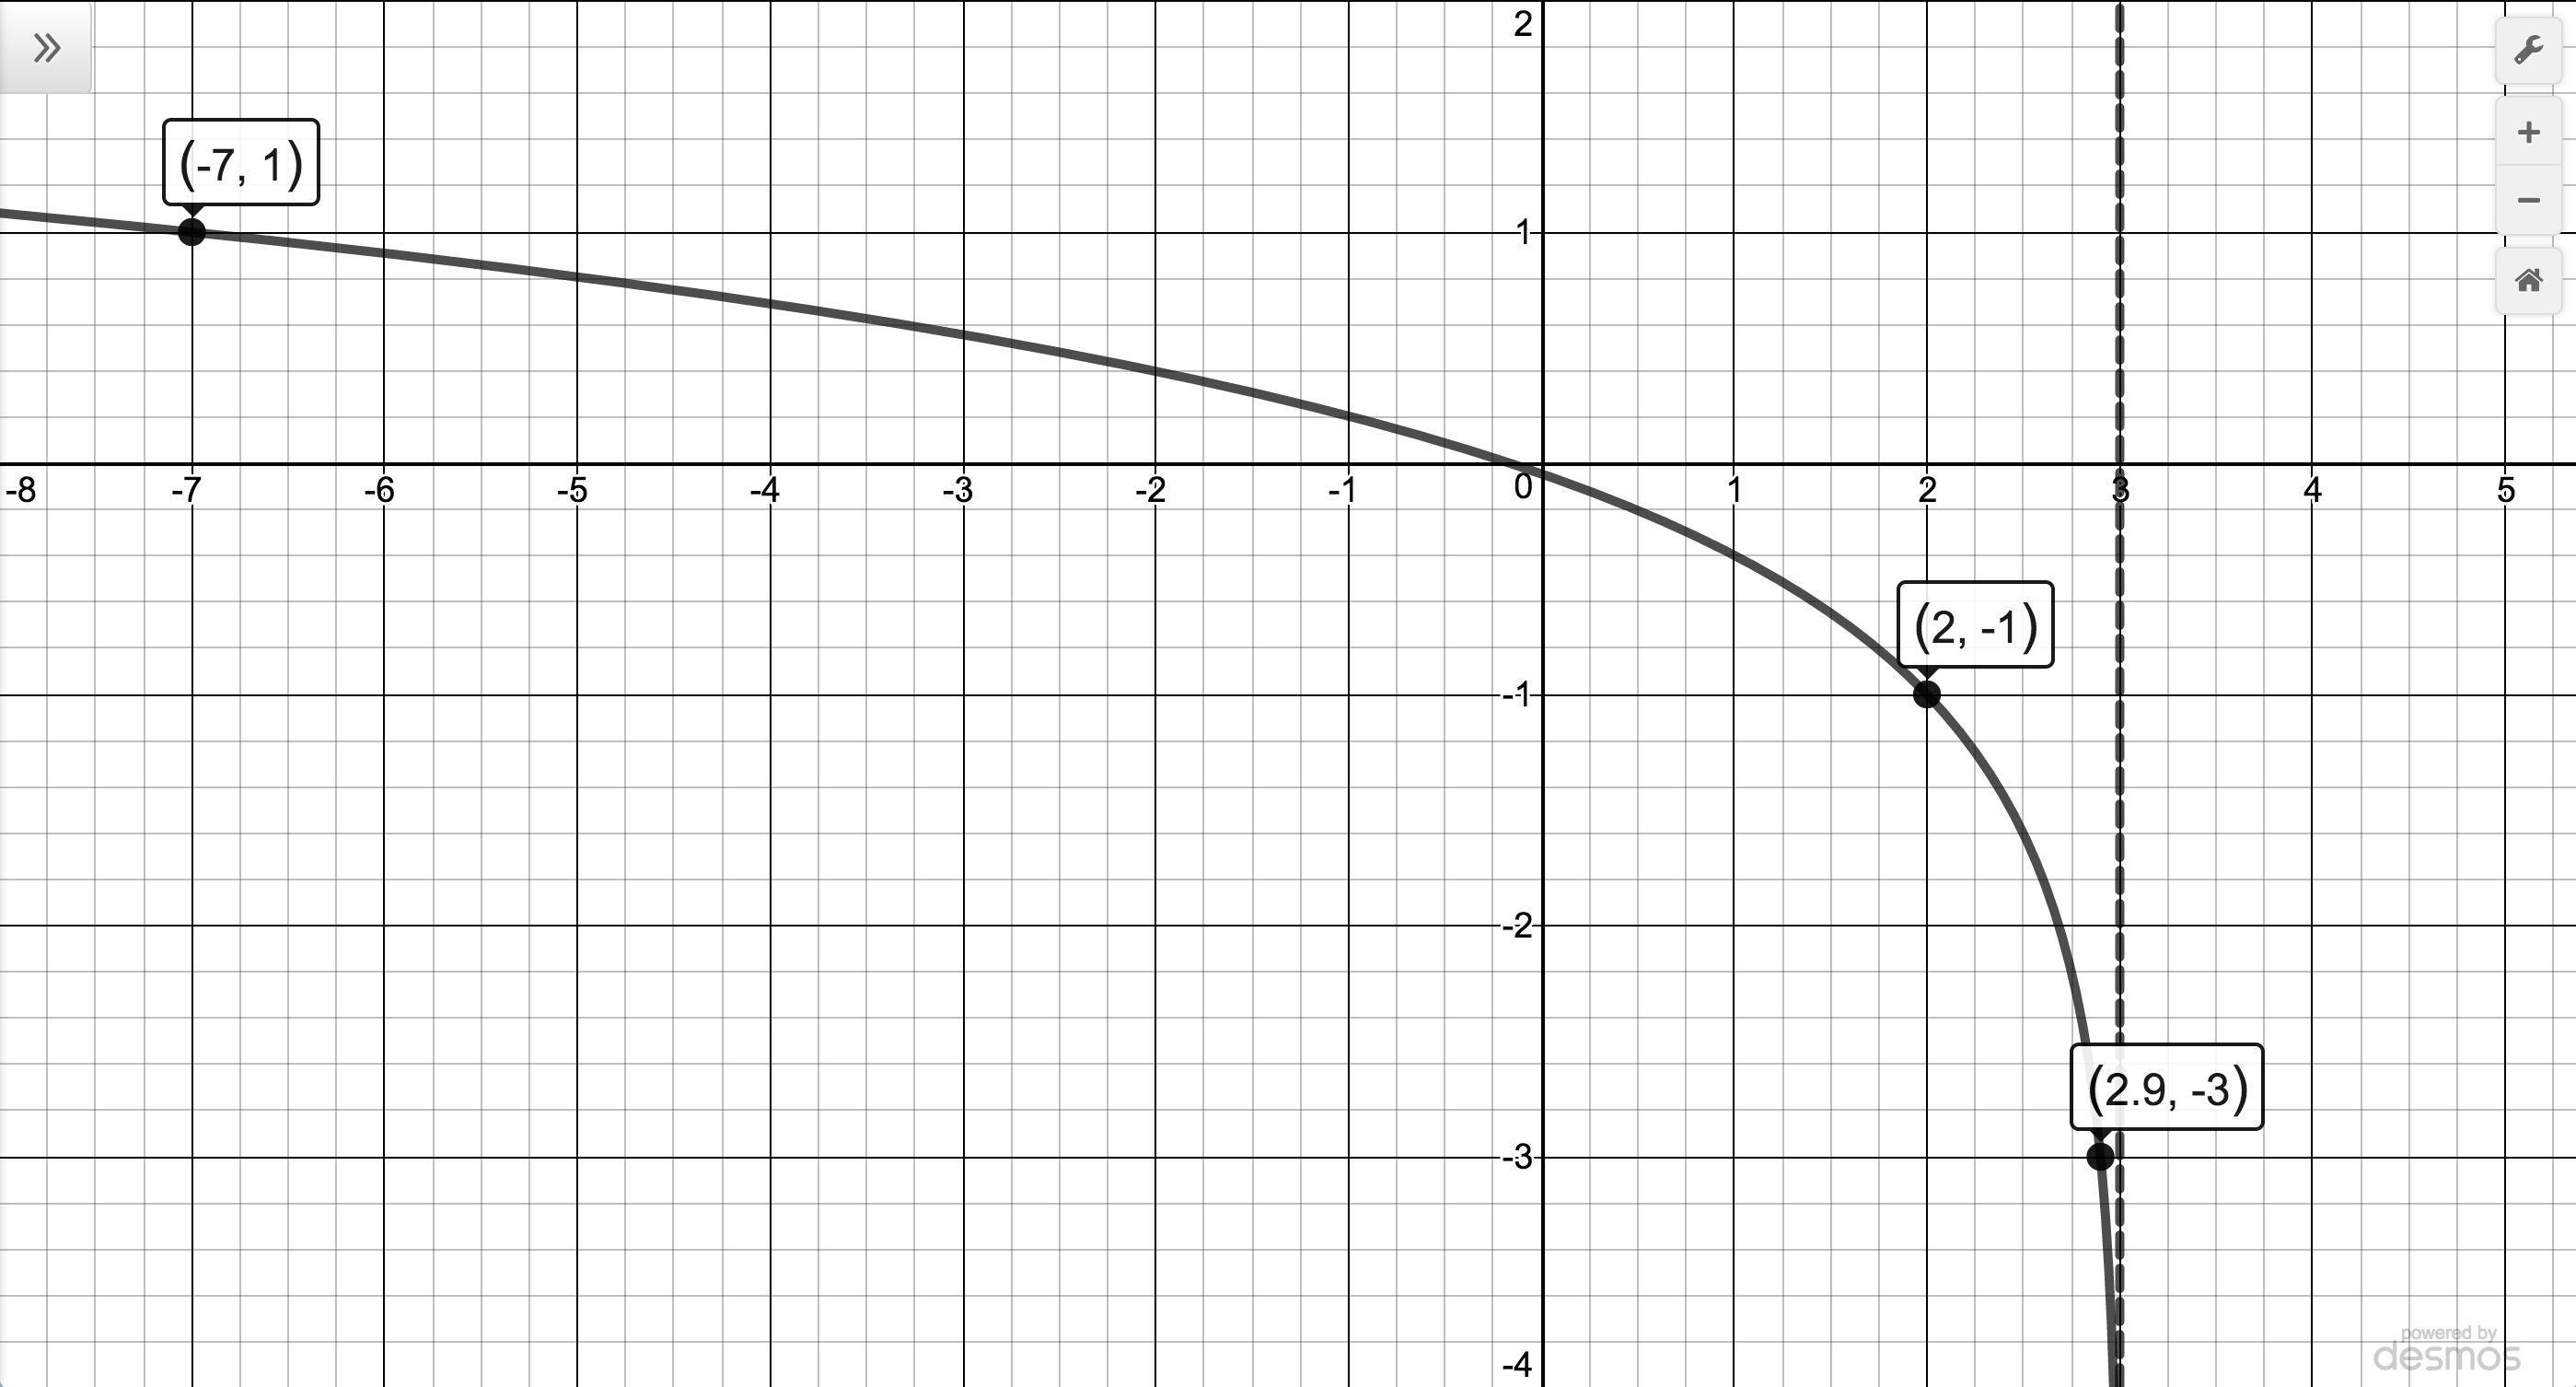
\includegraphics[height=2in]{./LogarithmicFunctionsGraphics/LogarithmicFunctionsEx01a.jpg}}

Note that in this case, we can graph $f$ using transformations, which we do so here for extra practice. 

\smallskip


Taking a cue from Theorem \ref{transformationsthm}, we rewrite $f(x) = 2 \log_{10}(-x+3) -1$ and  view this function as a transformed version of $h(x) = \log_{10}(x)$. 



\smallskip

To graph $y = \log(x) = \log_{10}(x)$,  We select three points to track corresponding to powers of $10$:  $(0.1, -1)$, $(1,0)$ and $(10,1)$, along with the vertical asymptote $x=0$.   


\smallskip

Since $f(x) = 2h(-x+3)-1$, Theorem \ref{transformationsthm} tells us that to obtain the destinations of these points, we first subtract $3$ from the $x$-coordinates (shifting the graph left $3$ units), then divide (multiply) by the $x$-coordinates by $-1$ (causing a reflection across the $y$-axis).   


\smallskip

Next, we multiply the $y$-coordinates by $2$ which results in a vertical stretch by a factor of $2$, then we finish by subtracting $1$ from the $y$-coordinates which shifts the graph down $1$ unit.  


\smallskip

Tracking points, we find:   $(0.1, -1) \rightarrow  (-2.9, -1) \rightarrow (2.9, -1) \rightarrow (2.9, -2) \rightarrow (2.9, -3)$, $(1,0) \rightarrow (-2,0) \rightarrow (2,0) \rightarrow (2,0) \rightarrow (2,-1)$, and  $(10,1) \rightarrow (7,1) \rightarrow (-7,1) \rightarrow (-7,2) \rightarrow (-7,1)$.  The vertical shift and reflection about the $y$-axis affects the vertical asymptote:  $x = 0 \rightarrow x = -3 \rightarrow x = 3$.  


\smallskip

Plotting these three points along with the vertical asymptote produces the graph of $f$ as seen above.


\item  To find the domain of $g$, we need to solve the inequality $\frac{x}{x-1} > 0$ using a sign diagram.\co{\footnote{See Section \ref{RationalGraphs} for a review of this process, if needed.}}

\smallskip

If we define $r(x) = \frac{x}{x-1}$, we find $r$ is undefined at $x=1$ and $r(x) = 0$ when $x=0$.  Choosing some test values, we generate the sign diagram below on the left.  

\smallskip

We find $ \frac{x}{x-1} > 0$ on $(-\infty, 0) \cup (1, \infty)$ which is the domain of  $g$. The graph below confirms this.


\begin{center}

\begin{multicols}{2}

\begin{mfpic}[10]{-5}{5}{-1}{2}
\arrow \reverse \arrow \polyline{(-5,0),(5,0)}
\xmarks{-2,2}
\tlabel[cc](-3.5,1){$(+)$}
\tlabel[cc](-2,-1){$0$}
\tlabel[cc](-2,1){$0$}
\tlabel[cc](0,1){$(-)$}
\tlabel[cc](2,-1){$1$}
\tlabel[cc](2,1){\textinterrobang}
\tlabel[cc](3.5,1){$(+)$}
\end{mfpic}

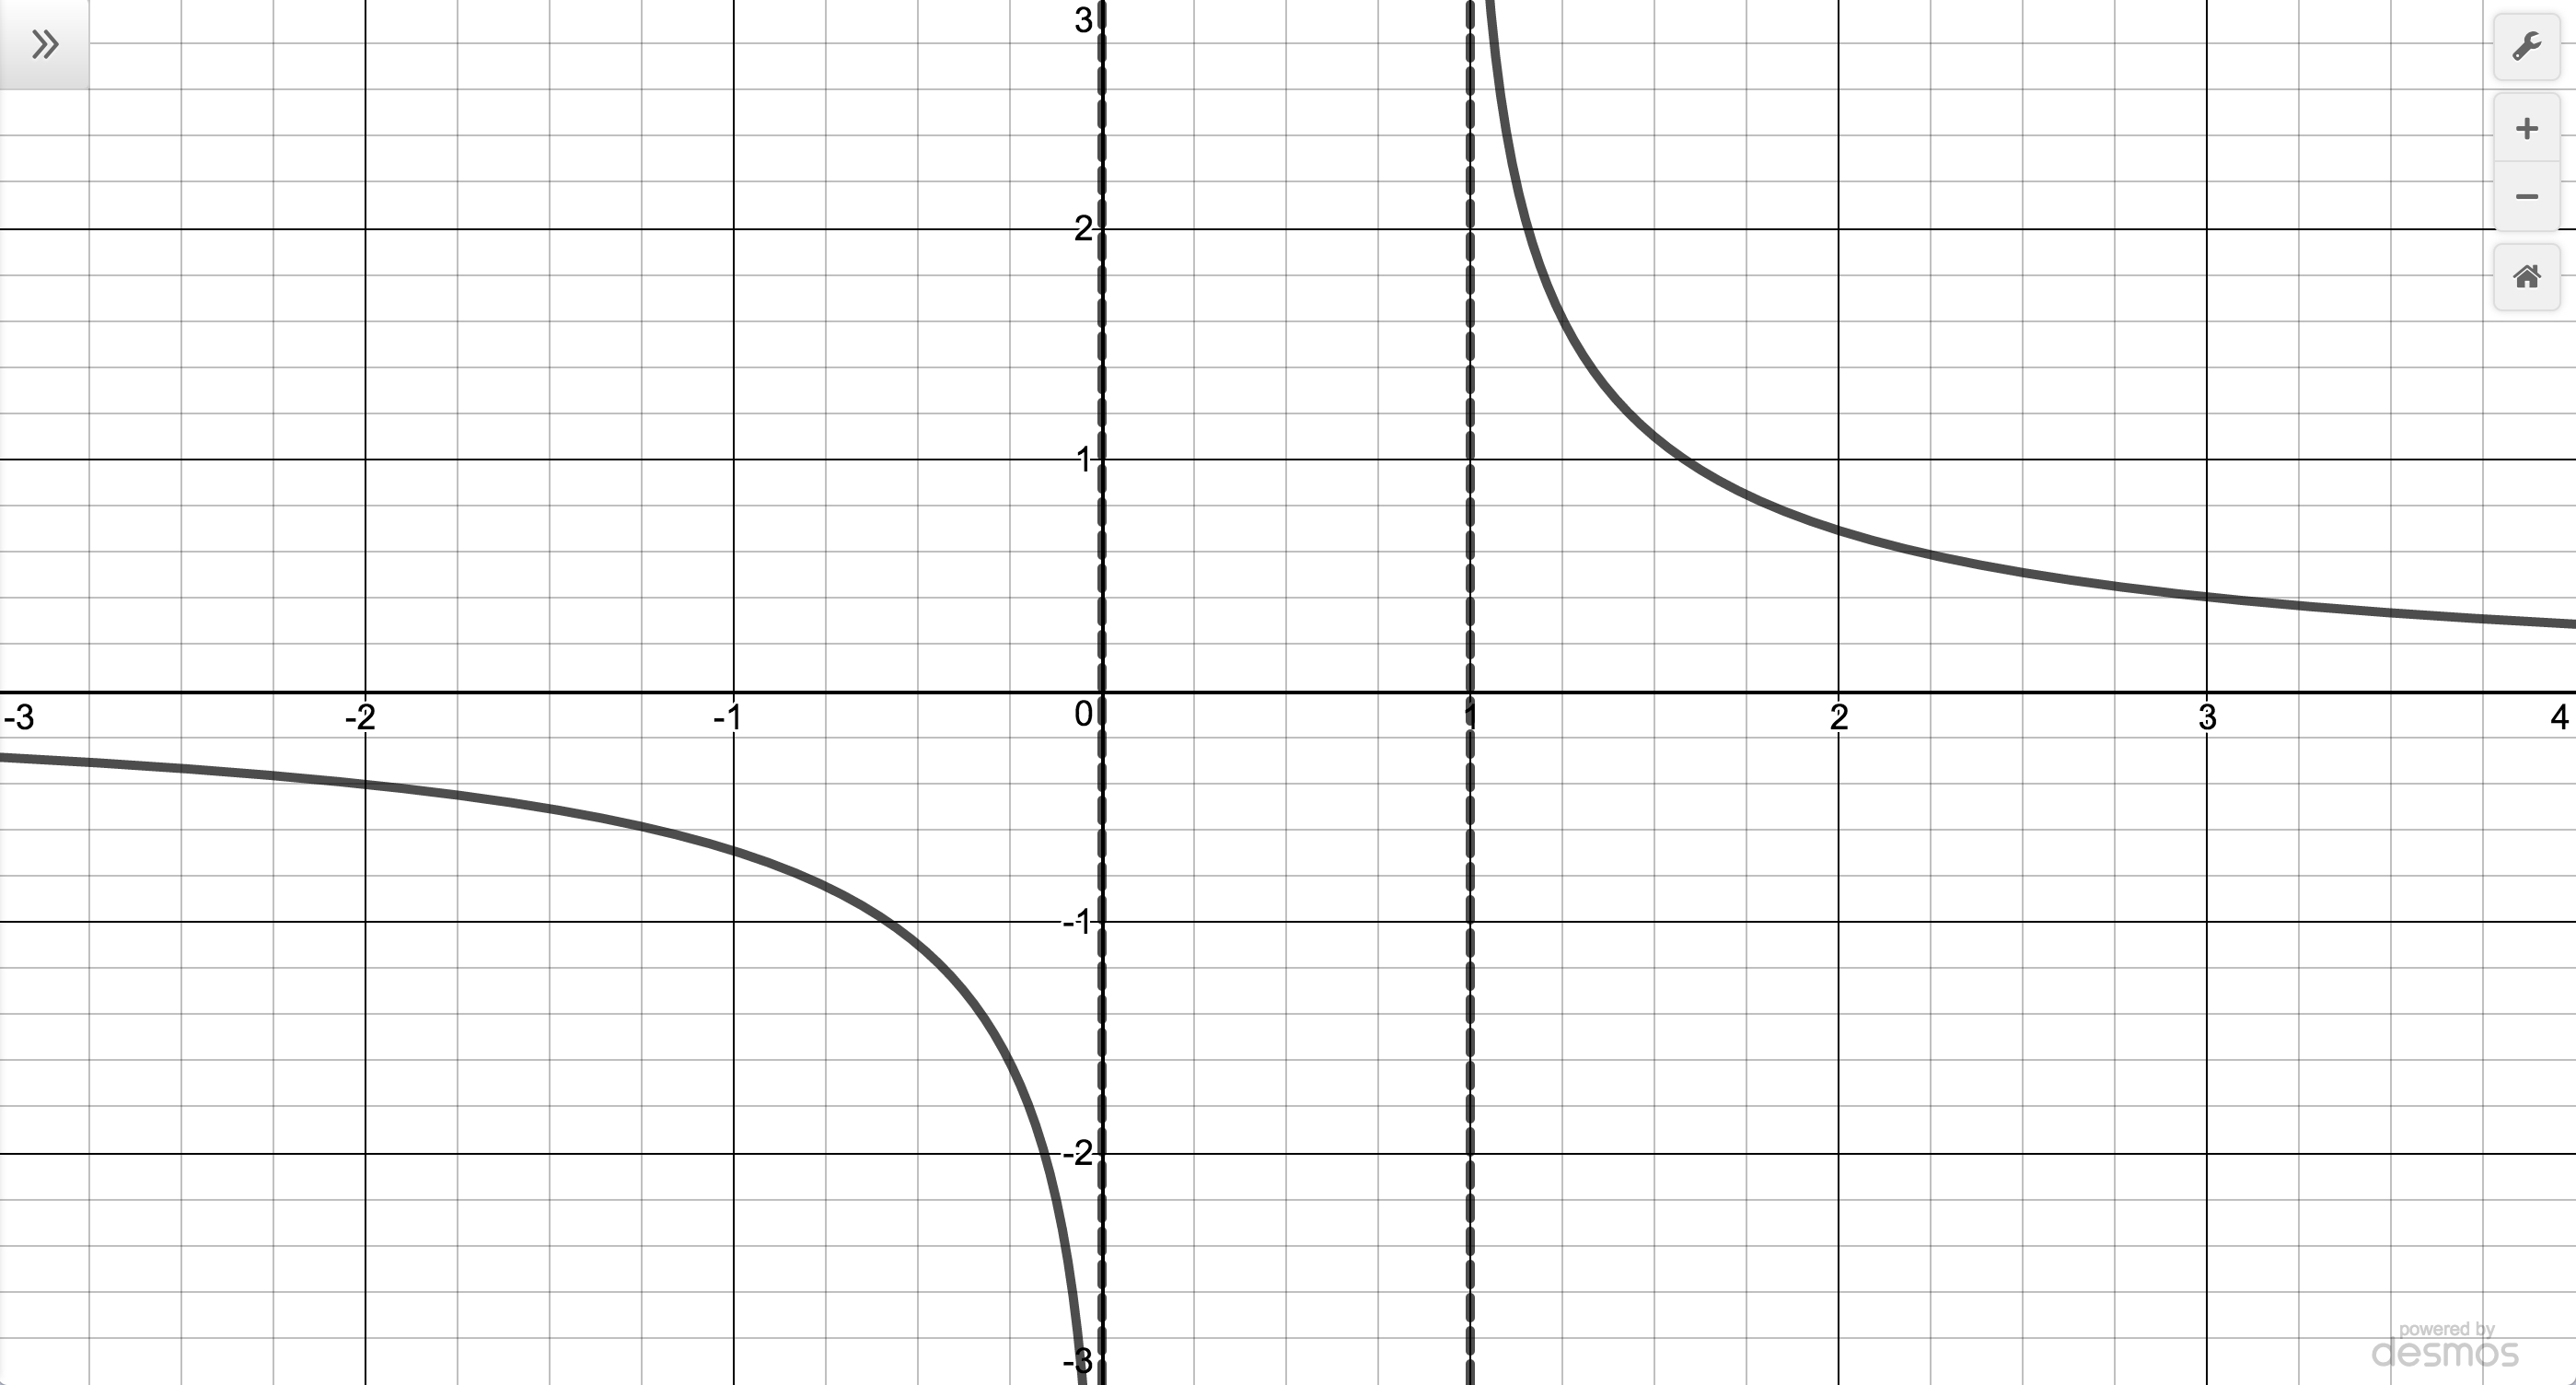
\includegraphics[width=3in]{./LogarithmicFunctionsGraphics/LogarithmicFunctionsEx01b.jpg}

\end{multicols}

\end{center}

  We can tell from the graph of $g$ that it is not the result of Section \ref{Transformations} transformations being applied to the graph $y = \ln(x)$, (do you see why?)  so barring a more detailed analysis using Calculus, producing a graph using a graphing utility is the best we can do.  
  
  \smallskip

One thing worthy of note, however, is the end behavior of $g$.  The graph suggests that as $x \rightarrow \pm \infty$, $g(x) \rightarrow 0$.  We can verify this analytically.  \co{Using results  from Chapter \ref{RationalFunctions} and continuity, w}We know that as $x \rightarrow \pm \infty$, $\frac{x}{x-1} \approx 1$.  Hence, it makes sense that $g(x) = \ln \left(\frac{x}{x-1}\right) \approx \ln(1) = 0$.  \qed

\end{enumerate}

\end{ex}

While logarithms have some interesting applications of their own which you'll explore in the exercises, their primary use to us will be to undo exponential functions. (This is, after all, how they were defined.)  Our last example  reviews not only the major topics of this section, but reviews the salient points from Section \ref{InverseFunctions}.

\newpage

\begin{ex}  Let $f(x) = 2^{x-1} - 3$. \label{proceduralinverse}

\begin{enumerate}

\item  Graph $f$ using transformations and state the domain and range of $f$.

\item  Explain why $f$ is invertible and find a formula for $f^{-1}(x)$.

\item  Graph $f^{-1}$ using transformations and state the domain and range of $f^{-1}$.

\item  Verify $\left(f^{-1} \circ f\right)(x) = x$ for all $x$ in the domain of $f$ and  $\left(f \circ f^{-1} \right)(x) = x$ for all $x$ in the domain of $f^{-1}$.

\item  Graph $f$ and $f^{-1}$ on the same set of axes and check for symmetry about the line $y = x$.

\item  Use $f$ or $f^{-1}$ to solve the following equations.  Check your answers algebraically.

\begin{multicols}{2}

\begin{enumerate}

\item  $2^{x-1} - 3 = 4$

\item  $\log_{2}(t+3)+1 = 0$

\end{enumerate}

\end{multicols}

\end{enumerate}

{\bf Solution.}  

\begin{enumerate}

\item   To graph $f(x) = 2^{x-1} - 3$ using  Theorem \ref{transformationsthm}, we first identify $g(x) = 2^{x}$ and note  $f(x) = g(x-1)-3$.  Choosing the `control points' of  $\left(-1, \frac{1}{2}\right)$, $(0,1)$ and $(1, 2)$ on the graph of $g$ along with the horizontal asymptote $y=0$, we implement the algorithm set forth in Theorem \ref{transformationsthm}.  

\smallskip

First, we first add $1$ to the $x$-coordinates of the points on the graph of $g$ which shifts the the graph of $g$ to the right one unit.   Next, we subtract $3$ from each of the $y$-coordinates on this new graph, shifting the graph down $3$ units to get the graph of $f$.

\smallskip

Looking point-by-point, we have  $\left(-1, \frac{1}{2}\right) \rightarrow \left(0, \frac{1}{2}\right) \rightarrow \left(0, -\frac{5}{2}\right)$,  $(0,1)  \rightarrow (1,1)  \rightarrow  (1,-2)$, and, finally, $(1, 2) \rightarrow (2, 2) \rightarrow (2, -1)$.  The horizontal asymptote is affected only by the vertical shift, $y = 0 \rightarrow y = -3$.  

\smallskip

From the graph of $f$, we get the domain is $(-\infty, \infty)$ and the range is $(-3, \infty)$.


\[\begin{array}{ccc}

\begin{mfpic}[15]{-4}{5}{-3.25}{8.25}
\axes
\tlabel[cc](5,-0.5){\scriptsize $x$}
\tlabel[cc](0.5,8.25){\scriptsize $y$}
\tcaption{\scriptsize $y = h(x) = 2^{x}$}
\xmarks{-3,-2,-1,1,2,3,4}
\ymarks{-3,-2,-1,1,2,3,4,5,6,7}
\tlpointsep{4pt}
\axislabels {x}{{\scriptsize $-3 \hspace{7pt}$} -3, {\scriptsize $-2 \hspace{7pt}$} -2, {\scriptsize $-1 \hspace{7pt}$} -1, {\scriptsize $1$} 1, {\scriptsize $2$} 2, {\scriptsize $3$} 3, {\scriptsize $4$} 4}
\axislabels {y}{{\scriptsize $-3$} -3, {\scriptsize $-2$} -2, {\scriptsize $-1$} -1,{\scriptsize $1$} 1, {\scriptsize $2$} 2, {\scriptsize $3$} 3, {\scriptsize $4$} 4, {\scriptsize $5$} 5, {\scriptsize $6$} 6, {\scriptsize $7$} 7}
\penwd{1.25pt}
\arrow \reverse \arrow \function{-3.5, 3, 0.1}{2**x}
\point[4pt]{(-1,0.5), (0,1), (1,2)}
\end{mfpic}

&

\xrightarrow{\hspace{1in}}

&

\begin{mfpic}[15]{-4}{5}{-3.25}{8.25}
\axes
\dashed \polyline{(-4,-3),(5,-3)}
\tlabel[cc](5,-0.5){\scriptsize $x$}
\tlabel[cc](0.5,8.25){\scriptsize $y$}
\tcaption{\scriptsize $y = f(x) = 2^{x-1}-3$}
\xmarks{-3,-2,-1,1,2,3,4}
\ymarks{-3,-2,-1,1,2,3,4,5,6,7}
\tlpointsep{4pt}
\axislabels {x}{{\scriptsize $-3 \hspace{7pt}$} -3, {\scriptsize $-2 \hspace{7pt}$} -2, {\scriptsize $-1 \hspace{7pt}$} -1, {\scriptsize $1$} 1, {\scriptsize $2$} 2, {\scriptsize $3$} 3, {\scriptsize $4$} 4}
\axislabels {y}{{\scriptsize $-2$} -2, {\scriptsize $-1$} -1,{\scriptsize $1$} 1, {\scriptsize $2$} 2, {\scriptsize $3$} 3, {\scriptsize $4$} 4, {\scriptsize $5$} 5, {\scriptsize $6$} 6, {\scriptsize $7$} 7}
\penwd{1.25pt}
\arrow \reverse \arrow \function{-2.5, 4, 0.1}{(2**(x-1))-3}
\point[4pt]{(0,-2.5), (1,-2), (2,-1)}
\end{mfpic} \\

\end{array}\]

\item  The graph of $f$ passes the Horizontal Line Test so $f$ is one-to-one, hence invertible.  

\smallskip

To find a formula for $f^{-1}(x)$, we normally set $y=f(x)$, interchange the $x$ and $y$, then proceed to solve for $y$.  Doing so in this situation leads us to the equation $x = 2^{y-1}-3$.  We have yet to discuss how to solve this kind of equation, so we will attempt to find the formula for $f^{-1}$ procedurally.  

\smallskip

Thinking of $f$ as a process, the formula $f(x) = 2^{x-1}-3$ takes an input $x$ and applies the steps: first subtract $1$.   Second put the result of the first step as the exponent on $2$.   Last, subtract $3$ from the result of the second step.

\smallskip

Clearly, to undo subtracting $1$, we will add $1$, and similarly we undo subtracting $3$ by adding $3$.  How do we undo the second step?  The answer is we use the logarithm.  

\smallskip

By definition, $\log_{2}(x)$ undoes exponentiation by $2$.  Hence, $f^{-1}$ should: first,  add $3$.  Second,  take the logarithm base $2$ of the result of the first step. Lastly,  add $1$ to the result of the second ste.  In symbols, $f^{-1}(x) = \log_{2}(x+3)+1$.  


\item  To graph $f^{-1}(x) = \log_{2}(x+3)+1$ using Theorem \ref{transformationsthm}, we start with $j(x) = \log_{2}(x)$ and track the points $\left(\frac{1}{2},-1\right)$, $(1,0)$ and $(2, 1)$ on the graph of $j$ along with the vertical asymptote $x=0$ through the transformations.

\smallskip

Since $f^{-1}(x) = j(x+3)+1$, we first subtract $3$ from each of the $x$-coordinates of each of the points on the graph of $y=j(x)$ shifting the graph of $j$ to the left three units.  We then add $1$ to each of the $y$-coordinates of the points on this new graph, shifting the graph up one unit. 

\smallskip

Tracking points, we get   $\left(\frac{1}{2},-1\right) \rightarrow \left(-\frac{5}{2},-1\right) \rightarrow \left(-\frac{5}{2},0\right)$, $(1,0) \rightarrow (-2,1) \rightarrow (-2,2)$, and $(2, 1) \rightarrow (-1, 1) \rightarrow (-1, 2)$.  

\smallskip

The vertical asymptote is only affected by the horizontal shift, so we have $x = 0 \rightarrow x = -3$.

\smallskip

From the graph below, we  get the  domain of $f^{-1}$ is $(-3, \infty)$, which matches the range of $f$, and the range of $f^{-1}$ is $(-\infty, \infty)$, which matches the domain of $f$, in accordance with Theorem \ref{inversefunctionprops}.

\[\begin{array}{ccc}

\begin{mfpic}[15]{-4}{9}{-4}{5}

\axes
\tlabel[cc](9,-0.5){\scriptsize $x$}
\tlabel[cc](0.5,5){\scriptsize $y$}
\tcaption{\scriptsize $y = j(x) = \log_{2}(x)$}
\ymarks{-3,-2,-1,1,2,3,4}
\xmarks{-3,-2,-1,1,2,3,4,5,6,7,8}
\tlpointsep{4pt}
\axislabels {y}{{\scriptsize $-3$} -3,{\scriptsize $-2$} -2, {\scriptsize $-1$} -1, {\scriptsize $1$} 1, {\scriptsize $2$} 2, {\scriptsize $3$} 3, {\scriptsize $4$} 4}
\axislabels {x}{{\scriptsize $-3 \hspace{7pt}$} -3, {\scriptsize $-2 \hspace{7pt}$} -2, {\scriptsize $-1 \hspace{7pt}$} -1,{\scriptsize $1$} 1, {\scriptsize $2$} 2, {\scriptsize $3$} 3, {\scriptsize $4$} 4, {\scriptsize $5$} 5, {\scriptsize $6$} 6, {\scriptsize $7$} 7, {\scriptsize $8$} 8}
\penwd{1.25pt}
\arrow \reverse \arrow \parafcn{-3.5, 3.1, 0.1}{(2**t,t)}
\point[4pt]{(0.5,-1), (1,0), (2,1)}
\end{mfpic}

&

\xrightarrow{\hspace{1in}}

&

\begin{mfpic}[15]{-4}{9}{-4}{5}
\axes
\tlabel[cc](9,-0.5){\scriptsize $x$}
\tlabel[cc](0.5,5){\scriptsize $y$}
\tcaption{\scriptsize $y = f^{-1}(x) = \log_{2}(x+3)+1$}
\ymarks{-3,-2,-1,1,2,3,4}
\xmarks{-3,-2,-1,1,2,3,4,5,6,7,8}
\tlpointsep{4pt}
\axislabels {y}{{\scriptsize $-3$} -3,{\scriptsize $-2$} -2, {\scriptsize $-1$} -1, {\scriptsize $1$} 1, {\scriptsize $2$} 2, {\scriptsize $3$} 3, {\scriptsize $4$} 4}
\axislabels {x}{{\scriptsize $-2 \hspace{7pt}$} -2, {\scriptsize $-1 \hspace{7pt}$} -1,{\scriptsize $1$} 1, {\scriptsize $2$} 2, {\scriptsize $3$} 3, {\scriptsize $4$} 4, {\scriptsize $5$} 5, {\scriptsize $6$} 6, {\scriptsize $7$} 7, {\scriptsize $8$} 8}
\dashed \polyline{(-3,-4),(-3,5)}
\penwd{1.25pt}
\point[4pt]{(-2.5,0), (-2,1), (-1,2)}
\arrow \reverse \arrow \parafcn{-2.5, 4.1, 0.1}{((2**(t-1))-3,t)}
\end{mfpic} \\

\end{array}\]

\item  We now verify that $f(x) = 2^{x-1}-3$ and $f^{-1}(x) = \log_{2}(x+3)+1$ satisfy the composition requirement for inverses.  When simplifying $(f^{-1} \circ f)(x)$ we assume $x$ can be any real number while when simplifying $(f \circ f^{-1})(x)$, we restrict our attention to $x > -3$. (Do you see why?)  

\smallskip

Note the use of the inverse properties of exponential and logarithmic functions  from Theorem \ref{logfcnprops} when it comes to simplifying expressions of the form $\log_{2}(2^{u})$ and $2^{\log_{2}(u)}$. 

\begin{multicols}{2}


$\begin{array}{rcl}

\left(f^{-1}\circ f\right)(x) & = & f^{-1}(f(x))  \\

& = & f^{-1}\left(2^{x-1}-3 \right)  \\

& = & \log_{2}\left( \left[2^{x-1}-3\right]+3 \right)+1  \\

& = & \log_{2}\left( 2^{x-1} \right)+1  \\

& = & (x-1) +1  \\

& = & x \, \, \checkmark \\

\end{array}$



$\begin{array}{rcl}

\left(f\circ f^{-1}\right)(x) & = & f\left(f^{-1}(x)\right) \\

& = & f\left( \log_{2}(x+3)+1 \right) \\

& = & 2^{\left( \log_{2}(x+3)+1 \right)-1} - 3 \\

& = & 2^{\log_{2}(x+3)} - 3  \\

& = & (x+3) -3  \\

& = & x \, \, \checkmark \\

\end{array}$

\end{multicols}


\item  Last, but certainly not least, we graph $y=f(x)$ and $y=f^{-1}(x)$ on the same set of axes and observe the symmetry about the line $y=x$.

\begin{center}
\begin{mfpic}[15]{-4}{7}{-4}{7}
\axes
\tlabel[cc](7,-0.5){\scriptsize $x$}
\tlabel[cc](0.5,7){\scriptsize $y$}
\tlabel(-4,-5){\scriptsize $y = f(x) = 2^{x-1}-3$}
\tlabel(-4,-6){\text{\scriptsize  \boldmath $y = f^{-1}(x) = \log_{2}(x+3)+1$}}
\xmarks{-3,-2,-1,1,2,3,4,5,6}
\ymarks{-3,-2,-1,1,2,3,4,5,6}
\tlpointsep{4pt}
\axislabels {x}{{\scriptsize $-3 \hspace{7pt}$} -3, {\scriptsize $-2 \hspace{7pt}$} -2, {\scriptsize $-1 \hspace{7pt}$} -1, {\scriptsize $1$} 1, {\scriptsize $2$} 2, {\scriptsize $3$} 3, {\scriptsize $4$} 4, {\scriptsize $5$} 5, {\scriptsize $6$} 6}
\axislabels {y}{{\scriptsize $-2$} -2, {\scriptsize $-1$} -1,{\scriptsize $1$} 1, {\scriptsize $2$} 2, {\scriptsize $3$} 3, {\scriptsize $4$} 4, {\scriptsize $5$} 5, {\scriptsize $6$} 6}
\arrow \reverse \arrow \function{-4.1, 4.1, 0.1}{(2**(x-1))-3}
\dashed \polyline{(-4,-3),(5,-3)}
\dashed \polyline{(-3,-3),(6,6)}
\dashed \polyline{(-3,-4),(-3,5)}
\penwd{1.5pt}
\arrow \reverse \arrow \parafcn{-4.1, 4.1, 0.1}{((2**(t-1))-3,t)}
\end{mfpic}

\end{center}
\end{enumerate}

\item  \begin{enumerate}

\item  Viewing $2^{x-1} - 3 = 4$ as $f(x) = 4$, we apply $f^{-1}$ to `undo' $f$ to get $f^{-1}(f(x)) = f^{-1}(4)$, which reduces to $x = f^{-1}(4)$.  Since we have shown (algebraically and graphically!) that $f^{-1}(x) =  \log_{2}(x+3) + 1$, we get  $x = f^{-1}(4) = \log_{2}(4+3) + 1 = \log_{2}(7) + 1$. 

\smallskip

Alternatively, we know from Theorem \ref{inversefunctionprops} that $f(x) = 4$ is equivalent to $x = f^{-1}(4)$ directly.

\smallskip


Note  that since, by definition,  $2^{\log_{2}(7)} = 7$,  $2^{( \log_{2}(7) + 1)-1} - 3 = 2^{\log_{2}(7)} - 3  = 7 - 3 = 4$, as required.

\item  Since we may think of the equation $\log_{2}(t+3)+1 = 0$ as $f^{-1}(t) = 0$, we can solve this equation by applying $f$ to both sides to get $f(f^{-1}(t)) = f(0)$ or $t = 2^{0-1} -3 = \frac{1}{2} - 3 = -\frac{5}{2}$.

Since $\log_{2}(2^{-1}) = -1$, we get  $\log_{2}\left(-\frac{5}{2} +3 \right)+1 = \log_{2}\left( \frac{1}{2} \right) + 1 =  \log_{2}(2^{-1})-1 + 1 = 0$, as required. \qed

\end{enumerate}

\end{ex}

\newpage

\subsection{Exercises}

\label{ExercisesforLogarithmicFunctions}

\label{IntroExpLogsExercises}

In Exercises \ref{rewritefirstex} - \ref{rewritelastex}, use the property: $b^{a} = c$ if and only if $\log_{b}(c) = a$ from Theorem \ref{logfcnprops} to rewrite the given equation in the other form.  That is, rewrite the exponential equations as logarithmic equations and rewrite the logarithmic equations as exponential equations.

\begin{multicols}{3}
\begin{enumerate}

\item  $2^{3} = 8$ \label{rewritefirstex}

\item  $5^{-3} = \frac{1}{125}$  

\item  $4^{5/2} = 32$  

\setcounter{HW}{\value{enumi}}
\end{enumerate}
\end{multicols}

\begin{multicols}{3}
\begin{enumerate}
\setcounter{enumi}{\value{HW}}

\item  $\left(\frac{1}{3}\right)^{-2} = 9$  

\item  $\left(\frac{4}{25}\right)^{-1/2} = \frac{5}{2}$  

\item  $10^{-3} = 0.001$ 

\setcounter{HW}{\value{enumi}}
\end{enumerate}
\end{multicols}

\begin{multicols}{3}
\begin{enumerate}
\setcounter{enumi}{\value{HW}}

\item  $e^{0}  = 1$  

\item  $\log_{5}(25) = 2$  

\item  $\log_{25} (5) = \frac{1}{2}$  

\setcounter{HW}{\value{enumi}}
\end{enumerate}
\end{multicols}

\begin{multicols}{3}
\begin{enumerate}
\setcounter{enumi}{\value{HW}}

\item  $\log_{3} \left(\frac{1}{81} \right) = -4$  

\item  $\log_{\frac{4}{3}} \left(\frac{3}{4} \right) = -1$  

\item  $\log(100) = 2$  

\setcounter{HW}{\value{enumi}}
\end{enumerate}
\end{multicols}

\begin{multicols}{3}
\begin{enumerate}
\setcounter{enumi}{\value{HW}}

\item  $\log (0.1) = -1$  

\item  $\ln(e) = 1$ 

\item  $\ln\left(\frac{1}{\sqrt{e}}\right) = -\frac{1}{2}$  \label{rewritelastex}

\setcounter{HW}{\value{enumi}}
\end{enumerate}
\end{multicols}

In Exercises \ref{simplifylogfirst} - \ref{simplifyloglast}, evaluate the expression without using a calculator.

\begin{multicols}{3}
\begin{enumerate}
\setcounter{enumi}{\value{HW}}

\item $\log_{3} (27)$  \label{simplifylogfirst}
\item $\log_{6} (216)$
\item $\log_{2} (32)$

\setcounter{HW}{\value{enumi}}
\end{enumerate}
\end{multicols}


\begin{multicols}{3}
\begin{enumerate}
\setcounter{enumi}{\value{HW}}

\item  $\log_{6} \left( \frac{1}{36} \right)$
\item $\log_{8} (4)$
\item $\log_{36} (216)$

\setcounter{HW}{\value{enumi}}
\end{enumerate}
\end{multicols}


\begin{multicols}{3}
\begin{enumerate}
\setcounter{enumi}{\value{HW}}

\item $\log_{\frac{1}{5}} (625)$
\item  $\log_{\frac{1}{6}} (216)$
\item $\log_{36} (36)$ 

\setcounter{HW}{\value{enumi}}
\end{enumerate}
\end{multicols}


\begin{multicols}{3}
\begin{enumerate}
\setcounter{enumi}{\value{HW}}

\item $\log \left(\frac{1}{1000000}\right)$
\item $\log(0.01)$
\item $\ln\left(e^3\right)$

\setcounter{HW}{\value{enumi}}
\end{enumerate}
\end{multicols}


\begin{multicols}{3}
\begin{enumerate}
\setcounter{enumi}{\value{HW}}

\item $\log_{4} (8)$
\item $\log_{6} (1)$
\item $\log_{13} \left(\sqrt{13}\right)$

\setcounter{HW}{\value{enumi}}
\end{enumerate}
\end{multicols}


\begin{multicols}{3}
\begin{enumerate}
\setcounter{enumi}{\value{HW}}

\item $\log_{36} \left(\sqrt[4]{36}\right)$
\item $7^{\log_{7} (3)}$
\item  $36^{\log_{36}(216)}$

\setcounter{HW}{\value{enumi}}
\end{enumerate}
\end{multicols}


\begin{multicols}{3}
\begin{enumerate}
\setcounter{enumi}{\value{HW}}

\item  $\log_{36} \left(36^{216}\right)$
\item $\ln \left(e^{5} \right)$
\item $\log \left(\sqrt[9]{10^{11}}\right)$

\setcounter{HW}{\value{enumi}}
\end{enumerate}
\end{multicols}


\begin{multicols}{3}
\begin{enumerate}
\setcounter{enumi}{\value{HW}}

\item  $\log\left( \sqrt[3]{10^5} \right)$
\item  $\ln \left( \frac{1}{\sqrt{e}}\right)$
\item $\log_{5} \left(3^{\log_{3} (5)}\right)$

\setcounter{HW}{\value{enumi}}
\end{enumerate}
\end{multicols}


\begin{multicols}{3}
\begin{enumerate}
\setcounter{enumi}{\value{HW}}

\item $\log\left(e^{\ln(100)}\right)$ 
\item $\log_{2}\left(3^{-\log_{3}(2)}\right)$
\item $\ln\left(42^{6\log(1)}\right)$ \label{simplifyloglast}

\setcounter{HW}{\value{enumi}}
\end{enumerate}
\end{multicols}

In Exercises \ref{domainlogfirst} - \ref{domainloglast}, find the domain of the function.

\begin{multicols}{2}
\begin{enumerate}
\setcounter{enumi}{\value{HW}}


\item $f(x) = \ln(x^{2} + 1)$ \label{domainlogfirst}
\item $f(x) = \log_{7}(4x + 8)$

\setcounter{HW}{\value{enumi}}
\end{enumerate}
\end{multicols}

\begin{multicols}{2}
\begin{enumerate}
\setcounter{enumi}{\value{HW}}


\item $g(t) = \ln(4t-20)$
\item $g(t) = \log \left(t^2+9t+18\right)$

\setcounter{HW}{\value{enumi}}
\end{enumerate}
\end{multicols}

\begin{multicols}{2}
\begin{enumerate}
\setcounter{enumi}{\value{HW}}

\item $f(x) = \log \left(\dfrac{x + 2}{x^{2} - 1}\right)$
\item $f(x) = \log\left(\dfrac{x^2+9x+18}{4x-20}\right)$

\setcounter{HW}{\value{enumi}}
\end{enumerate}
\end{multicols}

\begin{multicols}{2}
\begin{enumerate}
\setcounter{enumi}{\value{HW}}

\item $g(t) = \ln(7 - t) + \ln(t - 4)$
\item $g(t) = \ln(4t-20) + \ln\left(t^2+9t+18\right)$

\setcounter{HW}{\value{enumi}}
\end{enumerate}
\end{multicols}

\begin{multicols}{2}
\begin{enumerate}
\setcounter{enumi}{\value{HW}}

\item $f(x) = \log\left(x^2+x+1\right)$
\item $f(x) = \sqrt[4]{\log_{4} (x)}$

\setcounter{HW}{\value{enumi}}
\end{enumerate}
\end{multicols}

\begin{multicols}{2}
\begin{enumerate}
\setcounter{enumi}{\value{HW}}

\item $g(t) = \log_{9}(|t + 3| - 4)$
\item $g(t) = \ln(\sqrt{t - 4} - 3)$

\setcounter{HW}{\value{enumi}}
\end{enumerate}
\end{multicols}

\begin{multicols}{2}
\begin{enumerate}
\setcounter{enumi}{\value{HW}}

\item $f(x) = \dfrac{1}{3 - \log_{5} (x)}$
\item $f(x) = \dfrac{\sqrt{-1 - x}}{\log_{\frac{1}{2}} (x)}$

\setcounter{HW}{\value{enumi}}
\end{enumerate}
\end{multicols}

\begin{multicols}{2}
\begin{enumerate}
\setcounter{enumi}{\value{HW}}

\item $f(x) = \ln(-2x^{3} - x^{2} + 13x - 6)$  \label{domainloglast}

\setcounter{HW}{\value{enumi}}
\end{enumerate}
\end{multicols}


In Exercises \ref{graphlogfirst} - \ref{graphloglast}, sketch the graph of $y=g(x)$ by starting with the graph of $y = f(x)$ and using transformations.  Track at least three points of your choice and the vertical asymptote through the transformations. State the domain and range of $g$.


\begin{multicols}{2}
\begin{enumerate}
\setcounter{enumi}{\value{HW}}

\item  $f(x) = \log_{2}(x)$, $g(x) = \log_{2}(x+1)$ \label{graphlogfirst}

\item  $f(x) = \log_{\frac{1}{3}}(x)$, $g(x) = \log_{\frac{1}{3}}(x)+1$

\setcounter{HW}{\value{enumi}}
\end{enumerate}
\end{multicols}

\begin{multicols}{2}
\begin{enumerate}
\setcounter{enumi}{\value{HW}}


\item  $f(x) = \log_{3}(x)$, $g(x) = -\log_{3}(x-2)$

\item  $f(x) = \log(x)$, $g(x) = 2\log(x+20) -1$  

\setcounter{HW}{\value{enumi}}
\end{enumerate}
\end{multicols}

\begin{multicols}{2}
\begin{enumerate}
\setcounter{enumi}{\value{HW}}

\item  $g(t) = \log_{0.5}(t)$, $g(t) = 10 \log_{0.5}\left(\frac{t}{100}\right)$

\item  $g(t) = \log_{1.25}(t)$, $g(t) = \log_{1.25}(-t+1) + 2$

\setcounter{HW}{\value{enumi}}
\end{enumerate}
\end{multicols}

\begin{multicols}{2}
\begin{enumerate}
\setcounter{enumi}{\value{HW}}


\item  $g(t) = \ln(t)$, $g(t) = -\ln(8-t)$

\item  $g(t) = \ln(t)$, $g(t) = -10\ln\left(\frac{t}{10}\right)$ \label{graphloglast}

\setcounter{HW}{\value{enumi}}
\end{enumerate}
\end{multicols}

\begin{enumerate}
\setcounter{enumi}{\value{HW}}

\smallskip

\item  Verify that each function in Exercises \ref{graphlogfirst} - \ref{graphloglast} is the inverse of the corresponding function in Exercises \ref{graphexpfirsta} - \ref{graphexplasta} in Section \ref{ExponentialFunctions}.  (Match up \#\ref{graphexpfirsta} and \#\ref{graphlogfirst}, and so on.)

\setcounter{HW}{\value{enumi}}
\end{enumerate}

In Exercises, \ref{logformfirsta} - \ref{logformlasta}, the graph of a logarithmic function is given.  Find a formula for the function in the form $F(x) = a \cdot \log_{2}(bx-h)+k$.

\begin{multicols}{2}
\begin{enumerate}
\setcounter{enumi}{\value{HW}}

\item  \label{logformfirsta}  Points:  $\left( -\frac{5}{2}, -2 \right)$,  $\left(-2, -1 \right)$, $\left(-1,0 \right)$, \\
Asymptote:  $x = -3$. \\

\begin{mfpic}[13]{-4}{6}{-5}{3}
\axes
\tlabel[cc](6,-0.5){\scriptsize $x$}
\tlabel[cc](0.5,3){\scriptsize $y$}
\ymarks{-4, -3,-2,-1,1,2}
\xmarks{-3, -2, -1, 1,2,3,4,5}
\tlpointsep{4pt}
\axislabels {y}{{\scriptsize $-4$} -4,{\scriptsize $-3$} -3, {\scriptsize $-2$} -2, {\scriptsize $-1$} -1, {\scriptsize $1$} 1, {\scriptsize $2$} 2}
\axislabels {x}{{\scriptsize $1$} 1, {\scriptsize $2$} 2, {\scriptsize $3$} 3, {\scriptsize $4$} 4, {\scriptsize $5$} 5, {\scriptsize $-1 \hspace{7pt}$} -1, {\scriptsize $-2 \hspace{7pt}$} -2, {\scriptsize $-3 \hspace{7pt}$} -3}
\dashed \polyline{(-3,-5), (-3,3)}
\penwd{1.25pt}
\arrow \reverse \arrow \parafcn{-4.5, 2.1, 0.1}{( (2**(t+1))-3, t)}
\point[4pt]{(-2.5, -2), (-2,-1),(-1,0)}
\end{mfpic}

\vfill

\columnbreak

\item  Points:  $\left( 1, -1 \right)$, $\left( 2, 0 \right)$, $\left(\frac{5}{2}, 1 \right)$ \\
Asymptote:  $x = 3$. \\

\begin{mfpic}[13]{-6}{4}{-4}{4}
\axes
\tlabel[cc](4,-0.5){\scriptsize $x$}
\tlabel[cc](0.5,4){\scriptsize $y$}
\ymarks{-3,-2,-1,1,2,3}
\xmarks{-5 step 1 until 3}
\tlpointsep{4pt}
\axislabels {y}{{\scriptsize $-3$} -3, {\scriptsize $-2$} -2, {\scriptsize $-1$} -1, {\scriptsize $1$} 1, {\scriptsize $2$} 2, {\scriptsize $3$} 3}
\axislabels {x}{{\scriptsize $1$} 1, {\scriptsize $2$} 2, {\scriptsize $3$} 3, {\scriptsize $-1 \hspace{7pt}$} -1, {\scriptsize $-2 \hspace{7pt}$} -2, {\scriptsize $-3 \hspace{7pt}$} -3, {\scriptsize $-4 \hspace{7pt}$} -4, {\scriptsize $-5 \hspace{7pt}$} -5}
\dashed \polyline{(3,-4), (3,4)}
\penwd{1.25pt}
\arrow \reverse \arrow \parafcn{-3, 3.1, 0.1}{(3-(2**(-t)), t)}
\point[4pt]{(1,-1), (2,0), ( 2.5,1)}
\end{mfpic}


\setcounter{HW}{\value{enumi}}
\end{enumerate}
\end{multicols}

\begin{multicols}{2}
\begin{enumerate}
\setcounter{enumi}{\value{HW}}

\item  Points:  $\left(\frac{1}{2}, \frac{5}{2} \right)$, $\left(1, 3 \right)$, $\left(2, \frac{7}{2} \right)$, \\
Asymptote:  $x = 0$. \\

\begin{mfpic}[13]{-1}{9}{-1}{5}
\axes
\tlabel[cc](9,-0.5){\scriptsize $x$}
\tlabel[cc](0.5,5){\scriptsize $y$}
\ymarks{1 step 1 until 4}
\xmarks{1 step 1 until 8}
\tlpointsep{4pt}
\axislabels {y}{{\scriptsize $1$} 1, {\scriptsize $2$} 2, {\scriptsize $3$} 3, {\scriptsize $4$} 4}
\axislabels {x}{{\scriptsize $1$} 1, {\scriptsize $2$} 2, {\scriptsize $3$} 3, {\scriptsize $4$} 4, {\scriptsize $5$} 5, {\scriptsize $6$} 6, {\scriptsize $7$} 7, {\scriptsize $8$} 8}
\penwd{1.25pt}
\arrow \reverse \arrow \parafcn{1.25, 4.55, 0.1}{(2**(2*t-6), t)}
\point[4pt]{(0.5, 2.5), (1,3), (2,3.5) }
\end{mfpic}

\vfill

\columnbreak

\item  Points:  $\left( 6, -\frac{1}{2} \right)$, $\left(3,0 \right)$, $\left( \frac{3}{2}, \frac{1}{2} \right)$, \\
Asymptote:  $x = 0$.   \\

\begin{mfpic}[13]{-1}{9}{-4}{4}
\axes
\tlabel[cc](9,-0.5){\scriptsize $x$}
\tlabel[cc](0.5,4){\scriptsize $y$}
\ymarks{-3,-2,-1,1,2,3}
\xmarks{1,2,3,4,5,6,7,8}
\tlpointsep{4pt}
\axislabels {y}{{\scriptsize $-3$} -3, {\scriptsize $-2$} -2, {\scriptsize $-1$} -1, {\scriptsize $1$} 1, {\scriptsize $2$} 2, {\scriptsize $3$} 3}
\axislabels {x}{{\scriptsize $1$} 1, {\scriptsize $2$} 2, {\scriptsize $3$} 3,  {\scriptsize $7$} 7, {\scriptsize $8$} 8}
\penwd{1.25pt}
\arrow \reverse \arrow \parafcn{-0.79, 2, 0.1}{(3*(2**(-2*t)), t)}
\point[4pt]{(6, -0.5), (3,0), (1.5, 0.5)}
\end{mfpic}


\label{logformlasta} 

\setcounter{HW}{\value{enumi}}
\end{enumerate}
\end{multicols}


\begin{enumerate}
\setcounter{enumi}{\value{HW}}


\item \label{logformbase4exercise} Find a formula for each graph in Exercises \ref{logformfirsta} - \ref{logformlasta} of the form $G(x) =  a \cdot \log_{4}(bx-h)+k$.

\setcounter{HW}{\value{enumi}}
\end{enumerate}

In Exercises \ref{inverselogexpfirst} - \ref{inverselogexplast},  find the inverse of the function from the `procedural perspective' discussed in Example \ref{proceduralinverse} and graph the function and its inverse on the same set of axes.

\begin{multicols}{2}
\begin{enumerate}
\setcounter{enumi}{\value{HW}}

\item $f(x) = 3^{x + 2} - 4$  \label{inverselogexpfirst} 
\item $f(x) = \log_{4}(x - 1)$

\setcounter{HW}{\value{enumi}}
\end{enumerate}
\end{multicols}

\enlargethispage{.5in}
\vspace{-.2in}

\begin{multicols}{2}
\begin{enumerate}
\setcounter{enumi}{\value{HW}}

\item $g(t)= -2^{-t} + 1$
\item $g(t) = 5\log(t) - 2$ \label{inverselogexplast}

\setcounter{HW}{\value{enumi}}
\end{enumerate}
\end{multicols}

In Exercises \ref{decomposebasiclogfirst} - \ref{decomposebasicloglast}, write the given function as a nontrivial decomposition of functions as directed.

\begin{enumerate}
\setcounter{enumi}{\value{HW}}

\item  For $f(x) = \log_{2}(x+3) + 4$, find functions $g$ and $h$ so that $f=g+h$. \label{decomposebasiclogfirst}
\item  For $f(x) = \log(2x) - e^{-x}$, find functions $g$ and $h$ so that $f=g-h$. 
\item  For $f(t) = 3t \log(t)$, find functions $g$ and $h$ so that $f=gh$.
\item  For $r(x) = \dfrac{\ln(x)}{x}$, find functions $f$ and $g$ so $r = \dfrac{f}{g}$.
\item  For $k(t) = \ln(t^2+1)$, find functions $f$ and $g$  so that $k = g \circ f$.
\item  For $p(z) = (\ln(z))^2$, find functions $f$ and $g$ so $p = g \circ f$. \label{decomposebasicloglast}

\setcounter{HW}{\value{enumi}}
\end{enumerate}

\phantomsection
\label{logarithmicscales}

(Logarithmic Scales) In Exercises \ref{Richterexercise} - \ref{pHexercise}, we introduce three widely used measurement scales which involve common logarithms: the Richter scale, the decibel scale and the pH scale.  The computations involved in all three scales are nearly identical so pay attention to the subtle differences. \index{logarithmic scales}

\begin{enumerate}
\setcounter{enumi}{\value{HW}}

\item \label{Richterexercise} \index{Richter Scale} \index{earthquake ! Richter Scale} Earthquakes are complicated events and it is not our intent to provide a complete discussion of the science involved in them.  Instead, we refer the interested reader to a solid course in Geology\footnote{Rock-solid, perhaps?} or the U.S. Geological Survey's Earthquake Hazards Program found \href{http://earthquake.usgs.gov/}{\underline{here}} and present only a simplified version of the \href{http://en.wikipedia.org/wiki/Richter_scale}{\underline{Richter scale}}.  The Richter scale measures the magnitude of an earthquake by comparing the amplitude of the seismic waves of the given earthquake to those of a ``magnitude 0 event'', which was chosen to be a seismograph reading of $0.001$ millimeters recorded on a seismometer 100 kilometers from the earthquake's epicenter.  Specifically, the magnitude of an earthquake is given by \[M(x) = \log \left(\dfrac{x}{0.001}\right)\] where $x$ is the seismograph reading in millimeters of the earthquake recorded 100 kilometers from the epicenter.  

\begin{enumerate}

\item Show that $M(0.001) = 0$.
\item Compute $M(80,000)$.
\item Show that an earthquake which registered 6.7 on the Richter scale had a seismograph reading ten times larger than one which measured 5.7.
\item Find two news stories about recent earthquakes which give their magnitudes on the Richter scale.  How many times larger was the seismograph reading of the earthquake with larger magnitude?

\end{enumerate}

\item \label{decibelexercise} \index{decibel} \index{sound intensity level ! decibel} While the decibel scale can be used in many disciplines,\footnote{See this  \href{http://en.wikipedia.org/wiki/Decibel}{\underline{webpage}} for more information.} we shall restrict our attention to its use in acoustics, specifically its use in measuring the intensity level of sound. The Sound Intensity Level $L$ (measured in decibels) of a sound intensity $I$ (measured in watts per square meter) is given by \[L(I) = 10\log\left( \dfrac{I}{10^{-12}} \right).\] Like the Richter scale, this scale compares $I$ to baseline: $10^{-12} \frac{W}{m^{2}}$ is the threshold of human hearing. 

\begin{enumerate}

\item Compute $L(10^{-6})$.
\item Damage to your hearing can start with short term exposure to sound levels around 115 decibels.  What intensity $I$ is needed to produce this level? 
\item Compute $L(1)$.  How does this compare with the threshold of pain which is around 140 decibels?

\end{enumerate}

\item \label{pHexercise} \index{pH} \index{acidity of a solution ! pH} \index{alkalinity of a solution ! pH} The pH of a solution is a measure of its acidity or alkalinity.  Specifically, $\mbox{pH} = -\log[\mbox{H}^{+}]$ where $[\mbox{H}^{+}]$ is the hydrogen ion concentration in moles per liter.  A solution with a pH less than 7 is an acid, one with a pH greater than 7 is a base (alkaline) and a pH of 7 is regarded as neutral.

\begin{enumerate}

\item The hydrogen ion concentration of pure water is $[\mbox{H}^{+}] = 10^{-7}$.  Find its pH.
\item Find the pH of a solution with $[\mbox{H}^{+}] = 6.3 \times 10^{-13}$.
\item The pH of gastric acid (the acid in your stomach) is about $0.7$.  What is the corresponding hydrogen ion concentration?

\end{enumerate}

\setcounter{HW}{\value{enumi}}
\end{enumerate}

\begin{enumerate}
\setcounter{enumi}{\value{HW}}

\item Use the definition of logarithm to explain why  $\log_{b} 1 = 0$ and $\log_{b} b = 1$ for every $b > 0, \; b \neq 1$.

\setcounter{HW}{\value{enumi}}
\end{enumerate}


\newpage

\subsection{Answers}

\begin{multicols}{3}
\begin{enumerate}

\item $\log_{2}(8) = 3$

\item  $\log_{5}\left(\frac{1}{125}\right) = -3$

\item  $\log_{4}(32) = \frac{5}{2}$

\setcounter{HW}{\value{enumi}}
\end{enumerate}
\end{multicols}

\begin{multicols}{3}
\begin{enumerate}
\setcounter{enumi}{\value{HW}}


\item  $\log_{\frac{1}{3}}(9) = -2$

\item  $\log_{\frac{4}{25}}\left(\frac{5}{2}\right) = -\frac{1}{2}$

\item  $\log(0.001) = -3$

\setcounter{HW}{\value{enumi}}
\end{enumerate}
\end{multicols}

\begin{multicols}{3}
\begin{enumerate}
\setcounter{enumi}{\value{HW}}


\item  $\ln(1) = 0$

\item  $5^{2} = 25$

\item  $(25)^{\frac{1}{2}} = 5$

\setcounter{HW}{\value{enumi}}
\end{enumerate}
\end{multicols}

\begin{multicols}{3}
\begin{enumerate}
\setcounter{enumi}{\value{HW}}


\item  $3^{-4} = \frac{1}{81}$

\item  $\left(\frac{4}{3} \right)^{-1} = \frac{3}{4}$

\item  $10^{2} = 100$

\setcounter{HW}{\value{enumi}}
\end{enumerate}
\end{multicols}

\begin{multicols}{3}
\begin{enumerate}
\setcounter{enumi}{\value{HW}}


\item  $10^{-1} = 0.1$

\item  $e^{1} = e$

\item  $e^{-\frac{1}{2}} = \frac{1}{\sqrt{e}}$

\setcounter{HW}{\value{enumi}}
\end{enumerate}
\end{multicols}

\begin{multicols}{3}
\begin{enumerate}
\setcounter{enumi}{\value{HW}}

\item $\log_{3} (27) = 3$
\item $\log_{6} (216) = 3$
\item $\log_{2} (32) = 5$

\setcounter{HW}{\value{enumi}}
\end{enumerate}
\end{multicols}

\begin{multicols}{3}
\begin{enumerate}
\setcounter{enumi}{\value{HW}}


\item  $\log_{6} \left( \frac{1}{36} \right) = -2$
\item $\log_{8} (4) = \frac{2}{3}$
\item $\log_{36} (216) = \frac{3}{2}$

\setcounter{HW}{\value{enumi}}
\end{enumerate}
\end{multicols}

\begin{multicols}{3}
\begin{enumerate}
\setcounter{enumi}{\value{HW}}


\item $\log_{\frac{1}{5}} (625) = -4$
\item  $\log_{\frac{1}{6}} (216) = -3$
\item $\log_{36} (36)=1$ 

\setcounter{HW}{\value{enumi}}
\end{enumerate}
\end{multicols}

\begin{multicols}{3}
\begin{enumerate}
\setcounter{enumi}{\value{HW}}


\item $\log \frac{1}{1000000} = -6$
\item $\log(0.01) = -2$
\item $\ln\left(e^3\right) = 3$

\setcounter{HW}{\value{enumi}}
\end{enumerate}
\end{multicols}

\begin{multicols}{3}
\begin{enumerate}
\setcounter{enumi}{\value{HW}}


\item $\log_{4} (8) = \frac{3}{2}$
\item $\log_{6} (1) = 0$
\item $\log_{13} \left(\sqrt{13}\right) = \frac{1}{2}$

\setcounter{HW}{\value{enumi}}
\end{enumerate}
\end{multicols}

\begin{multicols}{3}
\begin{enumerate}
\setcounter{enumi}{\value{HW}}


\item $\log_{36} \left(\sqrt[4]{36}\right) = \frac{1}{4}$
\item $7^{\log_{7} (3)} = 3$
\item  $36^{\log_{36}(216)} = 216$

\setcounter{HW}{\value{enumi}}
\end{enumerate}
\end{multicols}

\begin{multicols}{3}
\begin{enumerate}
\setcounter{enumi}{\value{HW}}


\item  $\log_{36} \left(36^{216}\right) = 216$
\item $\ln(e^{5}) = 5$
\item $\log \left(\sqrt[9]{10^{11}}\right) = \frac{11}{9}$

\setcounter{HW}{\value{enumi}}
\end{enumerate}
\end{multicols}

\begin{multicols}{3}
\begin{enumerate}
\setcounter{enumi}{\value{HW}}


\item  $\log\left( \sqrt[3]{10^5} \right) = \frac{5}{3}$
\item  $\ln \left( \frac{1}{\sqrt{e}}\right) = -\frac{1}{2} $
\item $\log_{5} \left(3^{\log_{3} 5}\right) = 1$

\setcounter{HW}{\value{enumi}}
\end{enumerate}
\end{multicols}

\begin{multicols}{3}
\begin{enumerate}
\setcounter{enumi}{\value{HW}}


\item $\log\left(e^{\ln(100)}\right) = 2$
\item $\log_{2}\left(3^{-\log_{3}(2)}\right) = -1$
\item $\ln\left(42^{6\log(1)}\right) = 0$

\setcounter{HW}{\value{enumi}}
\end{enumerate}
\end{multicols}


\begin{multicols}{3}
\begin{enumerate}
\setcounter{enumi}{\value{HW}}


\item $(-\infty, \infty)$
\item $(-2, \infty)$
\item $(5, \infty)$

\setcounter{HW}{\value{enumi}}
\end{enumerate}
\end{multicols}


\begin{multicols}{3}
\begin{enumerate}
\setcounter{enumi}{\value{HW}}


\item $(-\infty, -6) \cup (-3, \infty)$
\item $(-2, -1) \cup (1, \infty)$
\item $(-6,-3) \cup (5, \infty)$

\setcounter{HW}{\value{enumi}}
\end{enumerate}
\end{multicols}


\begin{multicols}{3}
\begin{enumerate}
\setcounter{enumi}{\value{HW}}


\item $(4, 7)$
\item $(5, \infty)$
\item $(-\infty, \infty)$

\setcounter{HW}{\value{enumi}}
\end{enumerate}
\end{multicols}


\begin{multicols}{3}
\begin{enumerate}
\setcounter{enumi}{\value{HW}}


\item $[1, \infty)$
\item $(-\infty, -7) \cup (1, \infty)$
\item $(13, \infty)$

\setcounter{HW}{\value{enumi}}
\end{enumerate}
\end{multicols}


\begin{multicols}{3}
\begin{enumerate}
\setcounter{enumi}{\value{HW}}


\item $(0, 125) \cup (125, \infty)$
\item No domain
\item $(-\infty, -3) \cup \left(\frac{1}{2}, 2\right)$

\setcounter{HW}{\value{enumi}}
\end{enumerate}
\end{multicols}

\newpage

\begin{multicols}{2}
\begin{enumerate}
\setcounter{enumi}{\value{HW}}


\item  Domain of $g$: $(-1, \infty)$\\
 Range of $g$:  $(-\infty, \infty)$ \\
 Points:  $\left( -\frac{1}{2}, -1 \right)$, $(0,0)$, $(1,1)$\\
 Asymptote: $x = -1$ \\

\begin{mfpic}[15]{-2}{9}{-4}{4}
\point[4pt]{(-0.5, -1), (0,0), (1,1)}
\axes
\tlabel[cc](0.5,4){\scriptsize $y$}
\tlabel[cc](9,-0.5){\scriptsize $x$}
\tlabel[cc](0.6, -3.1){\tiny $-3$}
\tlabel[cc](0.6, -2.1){\tiny $-2$}
\tlabel[cc](0.6, -1.1){\tiny $-1$}
\tcaption{$y = g(x) = \log_{2}(x+1)$}
\ymarks{-3,-2,-1,1,2,3}
\xmarks{-1,1,2,3,4,5,6,7,8}
\tlpointsep{4pt}
\axislabels {y}{{\tiny $1$} 1, {\tiny $2$} 2, {\tiny $3$} 3}
\axislabels {x}{{\tiny $1$} 1, {\tiny $2$} 2, {\tiny $3$} 3, {\tiny $4$} 4, {\tiny $5$} 5, {\tiny $6$} 6, {\tiny $7$} 7, {\tiny $8$} 8}
\dashed \polyline{(-1,-3),(-1,4)}
\penwd{1.25pt}
\arrow \reverse \arrow \parafcn{-3.5, 3.1, 0.1}{((2**(t))-1,t)}
\end{mfpic}

\vfill

\columnbreak

\item  Domain of $g$:  $(0, \infty)$\\
 Range of $g$:  $(-\infty, \infty)$ \\
 Points:   $\left(\frac{1}{3}, 2 \right)$, $(1,1)$, $(3,0)$ \\
 Asymptote:  $x = 0$ \\

\begin{mfpic}[15]{-1}{10}{-4}{4}
\point[4pt]{(3,0), (1,1), (0.3333,2)}
\axes
\tlabel[cc](0.5, 4){\scriptsize $y$}
\tlabel[cc](10,-0.5){\scriptsize $x$}
\tcaption{$y = g(x) = \log_{\frac{1}{3}}(x)+1$}
\ymarks{-3,-2,-1,1,2,3}
\xmarks{1,2,3,4,5,6,7,8,9}
\tlpointsep{4pt}
\axislabels {y}{{\tiny $-3$} -3, {\tiny $-2$} -2, {\tiny $-1$} -1, {\tiny $1$} 1, {\tiny $2$} 2, {\tiny $3$} 3}
\axislabels {x}{{\tiny $1$} 1, {\tiny $2$} 2, {\tiny $3$} 3, {\tiny $4$} 4, {\tiny $5$} 5, {\tiny $6$} 6, {\tiny $7$} 7, {\tiny $8$} 8, {\tiny $9$} 9}
\penwd{1.25pt}
\arrow \reverse \arrow \parafcn{-1.05, 3.5, 0.1}{(3**(1-t),t)}
\end{mfpic} 

\setcounter{HW}{\value{enumi}}
\end{enumerate}
\end{multicols}

\begin{multicols}{2}
\begin{enumerate}
\setcounter{enumi}{\value{HW}}


\item  Domain of $g$: $(2, \infty)$\\
 Range of $g$:  $(-\infty, \infty)$ \\
 Points:  $\left( \frac{7}{3},1 \right)$, $(3,0)$, $(5,-1)$ \\
 Asymptote: $x = 2$ \\
 
\begin{mfpic}[15]{-1}{12}{-4}{4}
\point[4pt]{(2.3333,1), (3,0), (5,-1)}
\axes
\tlabel[cc](0.5,4){\scriptsize $y$}
\tlabel[cc](12,-0.5){\scriptsize $x$}
\tcaption{$y = g(x) = -\log_{3}(x-2)$}
\ymarks{-3,-2,-1,1,2,3}
\xmarks{1,2,3,4,5,6,7,8,9,10,11}
\tlpointsep{4pt}
\axislabels {y}{{\tiny $-3$} -3, {\tiny $-2$} -2, {\tiny $-1$} -1, {\tiny $1$} 1, {\tiny $2$} 2, {\tiny $3$} 3}
\axislabels {x}{{\tiny $1$} 1, {\tiny $2$} 2, {\tiny $3$} 3, {\tiny $4$} 4, {\tiny $5$} 5, {\tiny $6$} 6, {\tiny $7$} 7, {\tiny $8$} 8, {\tiny $9$} 9, {\tiny $10$} 10, {\tiny $11$} 11}
\dashed \polyline{(2,-3),(2,4)}
\penwd{1.25pt}
\arrow \reverse \arrow \parafcn{-2.05, 2.5, 0.1}{(2+3**(0-t),t)}
\end{mfpic} 

\vfill

\columnbreak


\item  Domain of $g$: $(-20, \infty)$\\
 Range of $g$:  $(-\infty, \infty)$\\
 Points:  $(-19, -1)$, $(-10,1)$, $(80,3)$\\
 Asymptote:  $x = -20$ \\

\begin{mfpic}[15]{-2}{11}{-3}{4}
\point[4pt]{(-1.9,-1), (-1,1), (8,3)}
\axes
\tlabel[cc](0.5,4){\scriptsize $y$}
\tlabel[cc](11,-0.5){\scriptsize $x$}
\tcaption{$y = g(x) = 2\log(x+20) -1$}
\ymarks{-3,-2,-1,1,2,3}
\xmarks{-2,-1,1,2,3,4,5,6,7,8,9,10}
\tlpointsep{4pt}
\axislabels {y}{{\tiny $-3$} -3, {\tiny $-2$} -2, {\tiny $-1$} -1, {\tiny $1$} 1, {\tiny $2$} 2, {\tiny $3$} 3}
\axislabels {x}{{\tiny $-10 \hspace{5pt}$} -1,{\tiny $10$} 1, {\tiny $20$} 2, {\tiny $30$} 3, {\tiny $40$} 4, {\tiny $50$} 5, {\tiny $60$} 6, {\tiny $70$} 7, {\tiny $80$} 8, {\tiny $90$} 9, {\tiny $100$} 10}
\dashed \polyline{(-2,-3), (-2,4)}
\penwd{1.25pt}
\arrow \reverse \arrow \parafcn{-3, 3.06, 0.1}{(((10**((t+1)/2))-20)/10,t)}
\end{mfpic}

\setcounter{HW}{\value{enumi}}
\end{enumerate}
\end{multicols}

\newpage

\begin{multicols}{2}
\begin{enumerate}
\setcounter{enumi}{\value{HW}}

\item  Domain of $g$: $(0, \infty)$ \\
  Range of $g$:  $(-\infty, \infty)$ \\
  Points:  $(50,10)$,   $(100,0)$, $(200,-10)$  \\
  Asymptote: $t= 0$\\
 
\begin{mfpic}[15]{-1}{9}{-4}{4}
\point[4pt]{(2,-1), (1,0), (0.5,1)}
\axes
\tlabel[cc](9,-0.5){\scriptsize $t$}
\tlabel[cc](0.5,4){\scriptsize $y$}
\tcaption{ $y = g(t) = 10 \log_{0.5} \left( \frac{t}{100} \right)$}
\ymarks{-3,-2,-1,1,2,3}
\xmarks{1,2,3,4,5,6,7,8}
\tlpointsep{4pt}
\axislabels {y}{{\tiny $-30$} -3, {\tiny $-20$} -2, {\tiny $-10$} -1, {\tiny $10$} 1, {\tiny $20$} 2, {\tiny $30$} 3}
\axislabels {x}{{\tiny $100$} 1, {\tiny $200$} 2, {\tiny $300$} 3, {\tiny $400$} 4, {\tiny $500$} 5, {\tiny $600$} 6, {\tiny $700$} 7, {\tiny $800$} 8}
\penwd{1.25pt}
\arrow \reverse \arrow \parafcn{-3, 3, 0.1}{(0.5**t, t)}
\end{mfpic}

\vfill

\columnbreak


\item  Domain of $g$: $(-\infty, 1)$ \\
  Range of $g$: $(-\infty, \infty)$  \\
  Points:  $(-0.25,3)$,  $(0,2)$, $(0.2,1)$ \\
  Asymptote: $t = 1$\\
 
\begin{mfpic}[8][10]{-11}{11}{-8}{5}
\point[4pt]{(2,1), (0,2), ( -2.5,3)}
\axes
\tlabel[cc](11,-0.5){\scriptsize $t$}
\tlabel[cc](0.5,5){\scriptsize $y$}
\tcaption{ $y = g(t) = \log_{1.25}(-t+1) + 2$}
\ymarks{-8 step 1 until 4}
\xmarks{-10 step 1 until 10}
\tlpointsep{4pt}
\axislabels {y}{{\tiny $-8$} -8,{\tiny $-6$} -6,{\tiny $-4$} -4,{\tiny $-2$} -2, {\tiny $2$} 2, {\tiny $4$} 4}
\axislabels {x}{ {\tiny $0.2$} 2,  {\tiny $0.4$} 4,  {\tiny $0.6$} 6, {\tiny $0.8$} 8, {\tiny $1$} 10, {\tiny $-0.2  \hspace{7pt}$} -2, {\tiny $-0.4  \hspace{7pt}$} -4,  {\tiny $-0.6  \hspace{7pt}$} -6, {\tiny $-0.8  \hspace{7pt}$} -8, {\tiny $-1  \hspace{7pt}$} -10}
 
\dashed \polyline{(10,-8), (10,5)}
\penwd{1.25pt}
\arrow \reverse \arrow \parafcn{-8, 5, 0.1}{((1- (1.25**(t-2)))*10,t)}
\end{mfpic}

\setcounter{HW}{\value{enumi}}
\end{enumerate}
\end{multicols}


\begin{multicols}{2}
\begin{enumerate}
\setcounter{enumi}{\value{HW}}


\item  Domain of $g$:  $(-\infty, 8)$\\
 Range of $g$:$(-\infty, \infty)$\\
 Points:  $(8-e, -1) \approx (5.28, -1)$,\\
 $(7,0)$, $(8 - e^{-1}, 1) \approx (7.63,1)$ \\
 Asymptote:  $t = 8$ \\

\begin{mfpic}[15]{-1}{9}{-4}{4}
\point[4pt]{(7.6321,1), (7,0), (5.282,-1)}
\axes
\tlabel[cc](0.5,4){\scriptsize $y$}
\tlabel[cc](9,-0.5){\scriptsize $t$}
\tcaption{$y = g(t) = -\ln(8-t)$}
\ymarks{-3,-2,-1,1,2,3}
\xmarks{1,2,3,4,5,6,7,8}
\tlpointsep{4pt}
\axislabels {y}{{\tiny $-3$} -3, {\tiny $-2$} -2, {\tiny $-1$} -1, {\tiny $1$} 1, {\tiny $2$} 2, {\tiny $3$} 3}
\axislabels {x}{{\tiny $1$} 1, {\tiny $2$} 2, {\tiny $3$} 3, {\tiny $4$} 4, {\tiny $5$} 5, {\tiny $6$} 6, {\tiny $7$} 7, {\tiny $8$} 8}
\dashed \polyline{(8,-3), (8,4)}
\penwd{1.25pt}
\arrow \reverse \arrow \parafcn{-2.25, 2, 0.1}{(8-exp(0-t),t)}
\end{mfpic} 

\vfill

\columnbreak

\item  Domain of $g$:  $(0, \infty)$\\
 Range of $g$:  $(-\infty, \infty)$\\
 Points:  $(10e^{-1}, 10) \approx (3.68. 10)$ \\
 $(10,0)$, $(10e, -10) \approx (27.18, -10)$ \\
 Asymptote: $t = 0$ \\

\begin{mfpic}[15]{-1}{9}{-4}{4}
\point[4pt]{(0.3679,1), (1,0), (2.718,-1)}
\axes
\tlabel[cc](0.5,4){\scriptsize $y$}
\tlabel[cc](9,-0.5){\scriptsize $t$}
\tcaption{$y = g(t) = -10\ln\left(\frac{t}{10}\right)$}
\ymarks{-3,-2,-1,1,2,3}
\xmarks{1,2,3,4,5,6,7,8}
\tlpointsep{4pt}
\axislabels {y}{{\tiny $-30$} -3,{\tiny $-20$} -2,{\tiny $-10$} -1, {\tiny $10$} 1, {\tiny $20$} 2, {\tiny $30$} 3}
\axislabels {x}{{\tiny $10$} 1, {\tiny $20$} 2, {\tiny $30$} 3, {\tiny $40$} 4, {\tiny $50$} 5, {\tiny $60$} 6, {\tiny $70$} 7, {\tiny $80$} 8}
\penwd{1.25pt}
\arrow \reverse \arrow \parafcn{-2.15, 2, 0.1}{(exp(0-t),t)}
\end{mfpic}

\setcounter{HW}{\value{enumi}}
\end{enumerate}
\end{multicols}

\newpage


\begin{multicols}{2}
\begin{enumerate}
\setcounter{enumi}{\value{HW}}
\addtocounter{enumi}{1}

\item $F(x) = \log_{2}(x+3) - 1$

\item  $F(x) = -\log_{2}(-x+3)$


\setcounter{HW}{\value{enumi}}
\end{enumerate}
\end{multicols}

\begin{multicols}{2}
\begin{enumerate}
\setcounter{enumi}{\value{HW}}


\item $F(x) = \frac{1}{2} \log_{2}(x) + 3$

\item  $F(x) = -\frac{1}{2} \log_{2} \left( \frac{x}{3} \right)$

\setcounter{HW}{\value{enumi}}
\end{enumerate}
\end{multicols}

\begin{enumerate}
\setcounter{enumi}{\value{HW}}

\item  In order, the formulas for $G(x)$ are:

\begin{multicols}{2}
\begin{itemize}

\item $G(x) = 2\log_{4}(x+3) - 1$

\item  $G(x) = -2\log_{4}(-x+3)$

\end{itemize}
\end{multicols}

\begin{multicols}{2}
\begin{itemize}

\item $G(x) =  \log_{4}(x) + 3$

\item  $G(x) = - \log_{4} \left( \frac{x}{3} \right)$

\end{itemize}
\end{multicols}


\setcounter{HW}{\value{enumi}}
\end{enumerate}

\begin{multicols}{2}
\begin{enumerate}
\setcounter{enumi}{\value{HW}}


\item $y = f(x) = 3^{x + 2} - 4$\\
{\boldmath $y = f^{-1}(x) = \log_{3}(x + 4) - 2$}\\

\begin{mfpic}[13.5]{-5}{7}{-5}{7}
\axes
\tlabel[cc](7,-0.5){\scriptsize $x$}
\tlabel[cc](0.5,7){\scriptsize $y$}
\xmarks{-4 step 1 until 6}
\ymarks{-4 step 1 until 6}
\tlpointsep{4pt}
\tiny
\axislabels {x}{{$-4 \hspace{7pt}$} -4, {$-3 \hspace{7pt}$} -3, {$-2 \hspace{7pt}$} -2, {$-1 \hspace{7pt}$} -1, {$1$} 1, {$2$} 2, {$3$} 3, {$4$} 4, {$5$} 5, {$6$} 6}
\axislabels {y}{{$-4$} -4, {$-3$} -3, {$-2$} -2, {$-1$} -1,{$1$} 1, {$2$} 2, {$3$} 3, {$4$} 4, {$5$} 5, {$6$} 6}
\normalsize
\arrow \reverse \arrow \function{-5, 0.15, 0.1}{(3**(x+2))-4}
\dashed \polyline{(-4,-5),(-4,7)}
\dashed \polyline{(-5,-5),(5,5)}
\dashed \polyline{(-5,-4),(7,-4)}
\penwd{1.5pt}
\arrow \reverse \arrow \function{-3.95, 7, 0.1}{(ln(x+4))/(ln(3.0)) - 2}
\end{mfpic}

\vfill

\columnbreak

\item $y = f(x) = \log_{4}(x - 1)$\\
{\boldmath $y = f^{-1}(x) = 4^{x} + 1$}\\

\begin{mfpic}[18]{-3}{7}{-3}{7}
\axes
\tlabel[cc](7,-0.5){\scriptsize $x$}
\tlabel[cc](0.5,7){\scriptsize $y$}
\xmarks{-2 step 1 until 6}
\ymarks{-2 step 1 until 6}
\tlpointsep{4pt}
\tiny
\axislabels {x}{{$-2 \hspace{7pt}$} -2, {$-1 \hspace{7pt}$} -1, {$1$} 1, {$2$} 2, {$3$} 3, {$4$} 4, {$5$} 5, {$6$} 6}
\axislabels {y}{{$-2$} -2, {$-1$} -1,{$1$} 1, {$2$} 2, {$3$} 3, {$4$} 4, {$5$} 5, {$6$} 6}
\normalsize
\arrow \reverse \arrow \function{1.03, 7, 0.1}{(ln(x-1))/(ln(4.0))}
\dashed \polyline{(-3,1),(7,1)}
\dashed \polyline{(1,7),(1,-3)}
\dashed \polyline{(-2,-2),(5,5)}
\penwd{1.5pt}
\arrow \reverse \arrow \function{-3, 1.25, 0.1}{(4**x) + 1}
\end{mfpic}

\setcounter{HW}{\value{enumi}}
\end{enumerate}
\end{multicols}


\begin{multicols}{2}
\begin{enumerate}
\setcounter{enumi}{\value{HW}}

\item $y = g(t) = -2^{-t} + 1$\\
{ \boldmath $y = g^{-1}(t) = -\log_{2}(-t+1)$} \\

\begin{mfpic}[22.5]{-3}{3}{-3}{3}
\axes
\tlabel[cc](3,-0.25){\scriptsize $t$}
\tlabel[cc](0.25,3){\scriptsize $y$}
\xmarks{-2 step 1 until 2}
\ymarks{-2 step 1 until 2}
\tlpointsep{4pt}
\tiny
\axislabels {x}{{$-2 \hspace{7pt}$} -2, {$-1 \hspace{7pt}$} -1, {$1$} 1, {$2$} 2}
\axislabels {y}{{$-2$} -2, {$-1$} -1,{$1$} 1, {$2$} 2}
\normalsize
\arrow \reverse \arrow \function{-2, 3, 0.1}{1-(2**(-x))}
\dashed \polyline{(-3,1),(3,1)}
\dashed \polyline{(1,-3),(1,3)}
\dashed \polyline{(-2.5,-2.5),(2.5,2.5)}
\penwd{1.5pt}
\arrow \reverse \arrow \function{-3, 0.87, 0.1}{-(ln(1-x))/(ln(2.0))}
\end{mfpic}


\vfill

\columnbreak

\item $y = g(t) = 5\log(t) - 2$\\
{\boldmath $y = g^{-1}(t) = 10^{\frac{t + 2}{5}}$}\\

\begin{mfpic}[13.5]{-5}{6}{-5}{6}
\axes
\tlabel[cc](6,-0.5){\scriptsize $t$}
\tlabel[cc](0.5,6){\scriptsize $y$}
\xmarks{-4 step 1 until 5}
\ymarks{-4 step 1 until 5}
\tlpointsep{4pt}
\tiny
\axislabels {x}{{$-4 \hspace{7pt}$} -4, {$-3 \hspace{7pt}$} -3, {$-2 \hspace{7pt}$} -2, {$-1 \hspace{7pt}$} -1, {$1$} 1, {$2$} 2, {$3$} 3, {$4$} 4, {$5$} 5}
\axislabels {y}{{$-4$} -4, {$-3$} -3, {$-2$} -2, {$-1$} -1,{$1$} 1, {$2$} 2, {$3$} 3, {$4$} 4, {$5$} 5}
\normalsize
\arrow \reverse \arrow \function{0.3, 6, 0.1}{((5*ln(x))/ln(10.0)) - 2}
\dashed \polyline{(-4,-4),(4,4)}
\penwd{1.5pt}
\arrow \reverse \arrow \function{-5, 1.8, 0.1}{10**((x+2)/5)}
\end{mfpic}

\setcounter{HW}{\value{enumi}}
\end{enumerate}
\end{multicols}

\begin{enumerate}
\setcounter{enumi}{\value{HW}}

\item  One solution is $g(x) = \log_{2}(x+3)$ and $h(x) = 4$.
\item  One solution is $g(x) = \log(2x)$ and $h(x) = e^{-x}$. 
\item  One solution is $g(t) = 3t$ and $h(t) = \log(t)$.
\item  One solution is $f(x) = \ln(x)$ and $g(x)=x$.
\item  One solution is $f(t) = t^2+1$ and $g(t) = \ln(t)$.
\item  One solution is $f(z) = \ln(z)$ and $g(z) = z^2$. 

\setcounter{HW}{\value{enumi}}
\end{enumerate}


\begin{enumerate}
\setcounter{enumi}{\value{HW}}


\item \begin{enumerate}

\item $M(0.001) = \log \left(\frac{0.001}{0.001} \right) = \log(1) = 0$.
\item $M(80,000) = \log \left(\frac{80,000}{0.001} \right) = \log(80,000,000) \approx 7.9$.

\end{enumerate}

\item \begin{enumerate}

\item $L(10^{-6}) = 60$ decibels.
\item $I = 10^{-.5} \approx 0.316$ watts per square meter.
\item Since $L(1) = 120$ decibels and $L(100) = 140$ decibels, a sound with intensity level 140 decibels has an intensity 100 times greater than a sound with intensity level 120 decibels.

\end{enumerate}

\item \begin{enumerate}

\item The pH of pure water is 7.
\item If $[\mbox{H}^{+}] = 6.3 \times 10^{-13}$ then the solution has a pH of 12.2.
\item $[\mbox{H}^{+}] = 10^{-0.7} \approx .1995$ moles per liter.

\end{enumerate}

\end{enumerate}

\closegraphsfile

\newpage

\section{Properties of Logarithms}

\mfpicnumber{1}

\opengraphsfile{PropertiesofLogarithms}

\setcounter{footnote}{0}

\label{PropertiesofLogarithms}

In Section \ref{LogarithmicFunctions}, we introduced the logarithmic functions as inverses of exponential functions and discussed a few of their functional properties from that perspective.  In this section, we explore the algebraic properties of logarithms.  Historically, these have played a huge role in the scientific development of our society since, among other things, they were used to develop analog computing devices called \href{http://en.wikipedia.org/wiki/Slide_rule}{\underline{slide rules}} which enabled scientists and engineers to perform accurate calculations leading to such things as space travel and the moon landing.  

\smallskip

As we shall see shortly, logs inherit analogs of all of the properties of exponents you learned in Elementary and Intermediate Algebra.  We first extract two properties from Theorem \ref{logfcnprops} to remind us of the definition of a logarithm as the inverse of an exponential function.
\smallskip

\colorbox{ResultColor}{\bbm

\begin{thm}[Properties of Logarithmic Functions]  \label{invpropslogs} 

Let $b > 0$, $b \neq 1$. \index{exponential function ! inverse properties of}\index{logarithm ! inverse properties of}

\vspace{-.1in}

\begin{itemize}

\item   $b^{a} = c$ if and only if $\log_{b}(c) = a$.   That is, $\log_{b}(c)$ is the exponent you put on $b$ to obtain $c$.

\item  $\log_{b} \left(b^{x}\right) = x$ for all $x$ and $b^{\log_{b}(x)} = x$ for all $x > 0$

\end{itemize}

\end{thm}

\ebm}

\smallskip

Next, we spell out what it means for exponential and logarithmic functions to be one-to-one.

\smallskip

\colorbox{ResultColor}{\bbm

\begin{thm}[One-to-one Properties of Exponential and Logarithmic Functions]  \label{explogsonetoone} 

Let $f(x) = b^{x}$ and $g(x) = \log_{b}(x)$ where $b>0$, $b\neq 1$.  Then $f$ and $g$ are one-to-one and  \index{exponential function ! one-to-one properties of}\index{logarithm ! one-to-one properties of}

\vspace{-.1in}

\begin{itemize}

\item  $b^{u} = b^{w}$ if and only if $u=w$ for all real numbers $u$ and $w$.

\item  $\log_{b}(u) = \log_{b}(w)$ if and only if $u=w$ for all real numbers $u > 0$, $w > 0$.

\end{itemize}

\end{thm}

\ebm}

\smallskip


Next, we re-state Theorem \ref{algpropexpfcns} for reference below.

\smallskip

\colorbox{ResultColor}{\bbm

\begin{thm}[Algebraic Properties of Exponential Functions] 

Let $f(x) = b^{x}$ be an exponential function ($b > 0$, $b\neq 1$) and let $u$ and $w$ be real numbers. \index{exponential function ! algebraic properties of}

\begin{itemize}

\item  \textbf{Product Rule:} \index{product rule ! for exponential functions} $f(u+w) = f(u) f(w)$.  In other words, $b^{u+w} = b^{u} b^{w}$

\item  \textbf{Quotient Rule:} \index{quotient rule ! for exponential functions} $f(u-w) = \dfrac{f(u)}{f(w)}$.  In other words, $b^{u-w} = \dfrac{b^{u}}{b^{w}}$

\item  \textbf{Power Rule:} \index{power rule ! for exponential functions} $\left(f(u)\right)^w = f(uw)$.  In other words, $\left(b^{u}\right)^{w} = b^{uw}$

\end{itemize}

\end{thm}

\ebm}

\smallskip

 To each of these properties of listed in Theorem \ref{algpropexpfcns}, there corresponds an analogous property of logarithmic functions.  We list these below in our next theorem.

\smallskip

\colorbox{ResultColor}{\bbm

\begin{thm}[Algebraic Properties of Logarithmic Functions]  \label{algproplogfcns} 
Let $g(x) =\log_{b}(x)$ be a logarithmic function ($b > 0$, $b\neq 1$) and let $u>0$ and $w>0$ be real numbers. \index{logarithm ! algebraic properties of}

\begin{itemize}

\item  \textbf{Product Rule:} \index{product rule ! for logarithms} $g(uw) = g(u)+ g(w)$.  In other words, $\log_{b}(uw) = \log_{b}(u) + \log_{b}(w)$

\item  \textbf{Quotient Rule:} \index{quotient rule ! for logarithms} $g\left(\dfrac{u}{w} \right) = g(u) - g(w)$.  In other words, $\log_{b} \left( \dfrac{u}{w} \right) = \log_{b}(u) - \log_{b}(w)$

\item  \textbf{Power Rule:} \index{power rule ! for logarithms} $g\left(u^{w}\right) =w g(u)$.  In other words, $\log_{b}\left(u^{w}\right) = w \log_{b}(u)$

\end{itemize}

\end{thm}

\ebm}

\smallskip

There are a couple of different ways to understand why Theorem \ref{algproplogfcns} is true.  For instance, consider  the product rule: $\log_{b}(uw) = \log_{b}(u) + \log_{b}(w)$.  

\smallskip

Let $a = \log_{b}(uw)$, $c = \log_{b}(u)$, and $d = \log_{b}(w)$.  Then, by definition, $b^{a} = uw$, $b^{c} = u$ and $b^{d} = w$.  Hence, $b^{a} = uw = b^{c} b^{d} = b^{c+d}$, so that $b^{a} = b^{c+d}$. 

\smallskip

By the one-to-one property of $b^{x}$,  $b^{a} = b^{c+d}$ gives $a = c+d$. In other words, $\log_{b}(uw) = \log_{b}(u) + \log_{b}(w)$.  The remaining properties are proved similarly.  

\smallskip

From a purely functional approach, we can see the properties in Theorem \ref{algproplogfcns} as an example of how inverse functions interchange the roles of inputs in outputs.  

\smallskip

For instance, the Product Rule for exponential functions given in Theorem  \ref{algpropexpfcns}, $f(u+w) = f(u)f(w)$, says that adding inputs results in multiplying outputs.   

\smallskip

Hence, whatever $f^{-1}$ is, it must take the products of outputs from $f$ and return them to the sum of their respective inputs.  Since the outputs from $f$ are the inputs to $f^{-1}$ and vice-versa, we have that that $f^{-1}$ must take products of its inputs to the sum of their respective outputs. This is precisely one way to interpret the Product Rule for Logarithmic functions:  $g(uw) = g(u) + g(w)$.  

\smallskip

The reader is encouraged to view the remaining properties listed in Theorem \ref{algproplogfcns} similarly.  

\smallskip

The following examples help build familiarity with these properties.  In our first example, we are asked to `expand' the logarithms.  This means that we read the properties in Theorem \ref{algproplogfcns} from left to right and rewrite products inside the log as sums outside the log, quotients inside the log as  differences outside the log, and powers inside the log as factors outside the log.\footnote{Interestingly enough, it is the exact \textit{opposite} process (which we will practice later) that is most useful in Algebra, the utility of expanding logarithms becomes apparent in Calculus.}

\smallskip


\begin{ex}  \label{expandlogex} Expand the following using the properties of logarithms and simplify.  Assume when necessary that all quantities represent positive real numbers.

\begin{multicols}{3}
\begin{enumerate}

\item $\log_{2}\left(\dfrac{8}{x}\right)$ \vphantom{$\ln \left(\dfrac{3}{ex}\right)^2$}

\item $\log_{0.1} \left(10 x^2 \right)$ \vphantom{$\ln \left(\dfrac{3}{ex}\right)^2$}

\item  $\ln \left(\dfrac{3}{et}\right)^2$

\setcounter{HW}{\value{enumi}}
\end{enumerate}
\end{multicols}

\begin{multicols}{3}
\begin{enumerate}
\setcounter{enumi}{\value{HW}}

\item  $\log \sqrt[3]{\dfrac{100 x^2}{yz^5}}$

\item \label{factorlogpropex} $\vphantom{\log \sqrt[3]{\dfrac{100 x^2}{yz^5}}} \log_{117}\left(x^2 - 4\right)$

\setcounter{HW}{\value{enumi}}
\end{enumerate}
\end{multicols}

%\newpage

{\bf Solution.}

\begin{enumerate}


\item  To expand $\log_{2}\left(\frac{8}{x}\right)$, we use the Quotient Rule identifying $u = 8$ and $w=x$ and simplify.

\setlength{\extrarowheight}{6pt}
\[ \begin{array}{rclr}

\log_{2}\left(\dfrac{8}{x}\right) & = &  \log_{2}(8) - \log_{2}(x) & \mbox{Quotient Rule} \\

& = &  3 - \log_{2}(x) & \mbox{Since $2^{3} = 8$} \\

& = & - \log_{2}(x) + 3 & \\

\end{array}\]

\setlength{\extrarowheight}{2pt}

\item   In the expression $\log_{0.1} \left(10 x^2 \right)$, we have a power (the $x^2$) and a product, and the question becomes which property, Power Rule or Product Rule to use first.

\smallskip

In order to use the Power Rule, the \textit{entire} quantity inside the log must be raised to the same exponent.  Since the exponent $2$ applies only to the $x$, we first apply the Product Rule with $u=10$ and $w=x^2$.  Once  the $x^2$ is by itself inside the log, we apply the Power Rule with $u=x$ and $w=2$.

\setlength{\extrarowheight}{6pt}
\[ \begin{array}{rclr}
\log_{0.1} \left(10 x^2 \right) & = &  \log_{0.1} (10) +  \log_{0.1} \left(x^2 \right) & \mbox{Product Rule} \\
                                & = &  \log_{0.1} (10)+ 2 \log_{0.1} (x) & \mbox{Power Rule} \\
                                & = &  -1 + 2 \log_{0.1} (x) & \mbox{Since $(0.1)^{-1} = 10$} \\
                                & = &  2 \log_{0.1} (x) - 1 & \\
                              
\end{array}\]
\setlength{\extrarowheight}{2pt}


\item  We have a power, quotient and product occurring in $\ln \left(\frac{3}{et}\right)^2$.  Since the exponent $2$ applies to the entire quantity inside the logarithm, we begin with the Power Rule with $u=\frac{3}{et}$ and $w = 2$.  

\smallskip

Next, we see the Quotient Rule is applicable, with $u=3$ and $w=et$, so we replace $\ln\left(\frac{3}{et}\right)$  with the quantity $\ln(3) - \ln(et)$. 

\smallskip

Since $\ln \left(\frac{3}{et}\right)$ is being multiplied by $2$, the entire quantity $\ln(3) - \ln(et)$ is multiplied by $2$.  

\smallskip

Finally, we apply the Product Rule with $u=e$ and $w=x$, and replace $\ln(et)$ with the quantity $\ln(e) + \ln(t)$, and simplify, keeping in mind that the natural log is log base $e$.

\setlength{\extrarowheight}{6pt}
\[ \begin{array}{rclr}

\ln \left(\dfrac{3}{et}\right)^2 & = & 2 \ln \left(\dfrac{3}{et}\right) & \mbox{Power Rule} \\
                                 & = & 2 \left[ \ln(3) - \ln(et) \right] & \mbox{Quotient Rule} \\
                                 & = & 2 \ln(3) - 2\ln(et) & \\
                                 & = & 2 \ln(3) - 2\left[\ln(e) + \ln(t)\right] & \mbox{Product Rule} \\
                                 & = & 2 \ln(3) - 2\ln(e) - 2 \ln(t) & \\
                                 & = & 2\ln(3) - 2 - 2 \ln(t) & \mbox{Since $e^{1} = e$} \\
                                 & = & - 2 \ln(t) + 2\ln(3) - 2 & \\
\end{array}\]
\setlength{\extrarowheight}{2pt}
                        

\item In Theorem \ref{algproplogfcns}, there is no mention of how to deal with radicals.  However, thinking back to Definition \ref{rationalexponentdefn}, we can rewrite the cube root as a $\frac{1}{3}$ exponent.  We begin by using the Power Rule\footnote{At this point in the text, the reader is encouraged to carefully read through each step and think of which quantity is playing the role of $u$ and which is playing the role of $w$ as we apply each property.}, and we keep in mind that the common log is log base $10$. 
\setlength{\extrarowheight}{6pt}
\[ \begin{array}{rclr}

\log \sqrt[3]{\dfrac{100 x^2}{yz^5}} & = & \log \left(\dfrac{100 x^2}{yz^5}\right)^{1/3} & \\ [10pt]
																		& = & \frac{1}{3} \log\left(\dfrac{100 x^2}{yz^5}\right) & \mbox{Power Rule} \\ [5pt]
																		& = & \frac{1}{3} \left[ \log\left(100x^2\right) - \log\left(yz^5\right) \right] & \mbox{Quotient Rule} \\ 
																		& = & \frac{1}{3}\log\left(100x^2\right) - \frac{1}{3}\log\left(yz^5\right) & \\
																		& = & \frac{1}{3}\left[ \log(100) + \log\left(x^2\right)\right] - \frac{1}{3} \left[ \log(y) + \log\left(z^5\right) \right] & \mbox{Product Rule} \\
																		& = & \frac{1}{3} \log(100) + \frac{1}{3} \log\left(x^2\right) - \frac{1}{3} \log(y) - \frac{1}{3} \log\left(z^5\right) \\
																		& = & \frac{1}{3} \log(100) + \frac{2}{3} \log(x) - \frac{1}{3} \log(y) - \frac{5}{3} \log(z) & \mbox{Power Rule} \\
																		& = & \frac{2}{3} + \frac{2}{3} \log(x) - \frac{1}{3} \log(y) - \frac{5}{3} \log(z) & \mbox{Since $10^2=100$} \\
																		& = &  \frac{2}{3} \log(x) - \frac{1}{3} \log(y) - \frac{5}{3} \log(z) + \frac{2}{3} & \\


\end{array} \]
\setlength{\extrarowheight}{2pt}

\item  At first it seems as if we have no means of simplifying $\log_{117}\left(x^2-4\right)$, since none of the properties of logs addresses the issue of expanding a difference \textit{inside} the logarithm.  However, we may factor $x^2 - 4 = (x+2)(x-2)$ thereby introducing a product which gives us license to use the Product Rule.  Assuming both $x+2>0$ and $x-2>0$, that is, $x >2$  we expand as follows.

\setlength{\extrarowheight}{4pt}
\[ \begin{array}{rclr}

\log_{117}\left(x^2-4\right) & = & \log_{117} \left[(x+2)(x-2)\right] & \mbox{Factor} \\
														 & = & \log_{117}(x+2) + \log_{117}(x-2) & \mbox{Product Rule} \\
\end{array}\]
\setlength{\extrarowheight}{2pt}
\qed

\end{enumerate}

\end{ex}

A couple of remarks about Example \ref{expandlogex} are in order.  First, if we take a step back and look at each problem in the foregoing example, a general rule of thumb to determine which log property to apply first when faced with a multi-step problem is to apply the logarithm properties in the  `reverse order of operations.'

\smallskip

For example, if we were to substitute a number for $x$ into the expression $\log_{0.1} \left(10 x^2 \right)$, we would first square the $x$, then multiply by $10$.  The last step is the multiplication, which tells us the first log property to apply is the Product Rule.  The last property of logarithm to apply would the be the power rule applied to $\log_{0.1}(x^2)$.

\smallskip

Second,  the equivalence $\log_{117}\left(x^2-4\right) = \log_{117}(x+2) + \log_{117}(x-2)$ is valid only if $x > 2$.  Indeed,  the functions $f(x) = \log_{117}\left(x^2-4\right)$ and $g(x) = \log_{117}(x+2) + \log_{117}(x-2)$ have different domains, and, hence, are different functions.\footnote{We leave it to the reader to verify the domain of $f$ is $(-\infty, -2) \cup (2,\infty)$ whereas the domain of $g$ is $(2,\infty)$.} In general, when using log properties to expand a logarithm, we may very well be restricting the domain as we do so. 

\smallskip

One last comment before we move to reassembling logs from their various bits and pieces. The authors are well aware of the propensity for some students to become overexcited and invent their own properties of logs like $\log_{117}\left(x^2-4\right) = \log_{117}\left(x^2\right) - \log_{117}(4)$, which simply isn't true, in general.  The unwritten\footnote{The authors relish the irony involved in writing what follows.} property of logarithms is that if it isn't written in a textbook, it probably isn't true.    

\begin{ex}  \label{contractlogex} Use the properties of logarithms to write the following as a single logarithm.

\begin{multicols}{2}
\begin{enumerate}

\item  $\log_{3}(x-1) - \log_{3}(x+1)$

\item  $\log(x) + 2\log(y) - \log(z)$

\setcounter{HW}{\value{enumi}}
\end{enumerate}
\end{multicols}

\begin{multicols}{2}
\begin{enumerate}
\setcounter{enumi}{\value{HW}}

\item  $4\log_{2}(x) + 3$

\item  $-\ln(t) - \frac{1}{2}$


\end{enumerate}
\end{multicols}

{\bf Solution.} Whereas in Example \ref{expandlogex} we read the properties in Theorem \ref{algproplogfcns} from left to right to expand logarithms, in this example we read them from right to left.

\begin{enumerate}

\item The difference of logarithms requires the Quotient Rule: $\log_{3}(x-1) - \log_{3}(x+1) = \log_{3}\left(\frac{x-1}{x+1}\right)$.

\item  In the expression, $\log(x) + 2\log(y) - \log(z)$, we have both a sum and difference of logarithms.  

Before we use the product rule to combine $\log(x) + 2\log(y)$, we note that we need to apply the Power Rule to rewrite the coefficient $2$ as the power on $y$.  We  then apply the Product and Quotient Rules as we move from left to right.
\setlength{\extrarowheight}{6pt}
\[ \begin{array}{rclr}

\log(x) + 2\log(y) - \log(z) & = & \log(x) + \log\left(y^2\right) - \log(z) & \mbox{Power Rule} \\ [6pt]
                             & = & \log\left(xy^2\right) - \log(z) & \mbox{Product Rule} \\ [10pt]
                             & = & \log\left( \dfrac{xy^2}{z}\right) & \mbox{Quotient Rule} \\
                             
                            
\end{array}\]
\setlength{\extrarowheight}{2pt}

\item  We begin rewriting $4\log_{2}(x) + 3$ by applying the Power Rule:  $4\log_{2}(x) = \log_{2}\left(x^4\right)$.

In order to continue, we need to rewrite $3$ as a logarithm base $2$.  From Theorem \ref{invpropslogs}, we know $3 = \log_{2}\left(2^3\right)$.  Rewriting $3$ this way paves the way to use the Product Rule.

\setlength{\extrarowheight}{4pt}
\[ \begin{array}{rclr}

4\log_{2}(x) + 3 & = & \log_{2}\left(x^4\right) + 3  & \mbox{Power Rule} \\ 
                             & = & \log_{2}\left(x^4\right) + \log_{2}\left(2^3\right)& \mbox{Since $3 = \log_{2}\left(2^3\right)$} \\
                             & = & \log_{2}\left(x^4\right) + \log_{2}(8)& \\
                             & = & \log_{2}\left( 8x^4\right) & \mbox{Product Rule} \\
                             
                            
\end{array}\]
\setlength{\extrarowheight}{2pt}

\item To get started with $-\ln(t) - \frac{1}{2}$, we rewrite  $-\ln(t)$ as $(-1) \ln(t)$.  We can then use the Power Rule to obtain $(-1)\ln(t) = \ln\left(t^{-1}\right)$.

As in the previous problem, in order to continue, we need to rewrite $\frac{1}{2}$ as a natural logarithm. Theorem \ref{invpropslogs} gives us $\frac{1}{2} = \ln\left(e^{1/2}\right) = \ln\left(\sqrt{e}\right)$.  Hence,

\setlength{\extrarowheight}{6pt}
\[ \begin{array}{rclr}

-\ln(t) - \frac{1}{2} & = & (-1)\ln(t) - \frac{1}{2}  &  \\ 
                             & = & \ln\left(t^{-1}\right) - \frac{1}{2} & \mbox{Power Rule} \\
                             & = & \ln\left(t^{-1}\right) - \ln\left(e^{1/2}\right)& \mbox{Since $\frac{1}{2} = \ln\left(e^{1/2}\right)$} \\
                             & = & \ln\left(t^{-1}\right) - \ln\left(\sqrt{e} \right)& \\ [6pt]
                             & = & \ln\left(\dfrac{t^{-1}}{\sqrt{e}}\right) & \mbox{Quotient Rule} \\ [10pt]
                             & = & \ln\left(\dfrac{1}{t\sqrt{e}}\right) &
\end{array}\]
\setlength{\extrarowheight}{2pt}

\end{enumerate}

\vspace{-.3in} \qed

\end{ex}

As we would expect, the rule of thumb for re-assembling logarithms is the opposite of what it was for dismantling them.  That is, to rewrite an expression as a single logarithm, we apply log properties following the usual order of operations:  first,  rewrite coefficients of logs as powers using the Power Rule, then rewrite addition and subtraction using the Product and Quotient Rules, respectively, as written from left to right.

\smallskip

Additionally, we find that using log properties in this fashion can increase the domain of the expression.  For example, we leave it to the reader to verify the domain of $f(x) = \log_{3}(x-1) - \log_{3}(x+1)$ is $(1,\infty)$ but the domain of $g(x) = \log_{3}\left(\frac{x-1}{x+1}\right)$ is $(-\infty, -1) \cup (1, \infty)$.  We'll need to keep this in mind in Section \ref{LogarithmicEquationsandInequalities} since such manipulations can result in extraneous solutions.

\smallskip

The two logarithm buttons commonly found on calculators are the `LOG' and `LN' buttons which correspond to the common and natural logs, respectively.  Suppose we wanted an approximation to $\log_{2}(7)$.  The answer should be a little less than $3$, (Can you explain why?) but how do we coerce the calculator into telling us a more accurate answer?  We need the following theorem.

\smallskip

\colorbox{ResultColor}{\bbm

\begin{thm}[Change of Base Formulas] \label{changeofbase}
Let $a,b >0$, $a,b \neq 1$. \index{change of base formulas} \index{exponential function ! change of base formula} \index{logarithm ! change of base formula}

\begin{itemize}

\item  $a^{x} = b^{x \log_{b}(a)}$ for all real numbers $x$.

\item  $\log_{a}(x) = \dfrac{\log_{b}(x)}{\log_{b}(a)}$ for all real numbers $x > 0$.

\end{itemize}

\end{thm}

\ebm}

\smallskip

To prove these formulas, consider $b^{x \log_{b}(a)}$. Using the Power Rule, we can rewrite $x \log_{b}(a)$ as $\log_{b}\left(a^{x}\right)$.  Following this with the Inverse Properties in Theorem \ref{invpropslogs}, we get \[ b^{x \log_{b}(a)} = b^{\log_{b}\left(a^{x}\right)} = a^{x}.\] 

 To verify the logarithmic form of the property, we use the Power Rule and an Inverse Property to get: 
 
  \[\log_{a}(x) \cdot \log_{b}(a) =  \log_{b} \left(a^{\log_{a}(x)}\right) = \log_{b}(x).\] 
  
 We get the result by dividing both sides of the equation $\log_{a}(x) \cdot \log_{b}(a)  =  \log_{b}(x)$ by  $\log_{b}(a)$.  
 
 \smallskip
 
 
 Of course, the authors can't help but point out the inverse relationship between these two change of base formulas.  To change the base of an exponential expression, we \textit{multiply} the \textit{input} by the factor $\log_{b}(a)$.  To change the base of a logarithmic expression, we \textit{divide} the \textit{output} by the factor $\log_{b}(a)$.  
 
 \smallskip
 
 
 While, in the grand scheme of things, both change of base formulas are really saying the same thing, the logarithmic form is the one usually encountered in Algebra while the exponential form isn't usually introduced until Calculus.

\smallskip

\begin{ex}  Use an appropriate change of base formula to convert the following expressions to ones with the indicated base.  Verify your answers using a graphing utility, as appropriate.
\begin{multicols}{2}
\begin{enumerate}

\item  $3^{2}$ to base $10$

\item  $2^{x}$ to base $e$

\setcounter{HW}{\value{enumi}}
\end{enumerate}
\end{multicols}

\begin{multicols}{2}
\begin{enumerate}
\setcounter{enumi}{\value{HW}}


\item $\log_{4}(5)$ to base $e$

\item $\ln(x)$ to base $10$

\end{enumerate}
\end{multicols}

{\bf Solution.}

\begin{enumerate}

\item  We apply the Change of Base formula with $a=3$ and $b=10$ to obtain $3^2 = 10^{2 \log(3)}$. Typing the latter into a graphing utility produces an answer of $9$ as seen below.

\item  Here, $a=2$ and $b = e$ so we have $2^{x} = e^{x \ln(2)}$.  Using a graphing utility, we find the graphs of $f(x) = 2^x$ and $g(x) = e^{x \ln(2)}$ appear to overlap perfectly.

\begin{center}

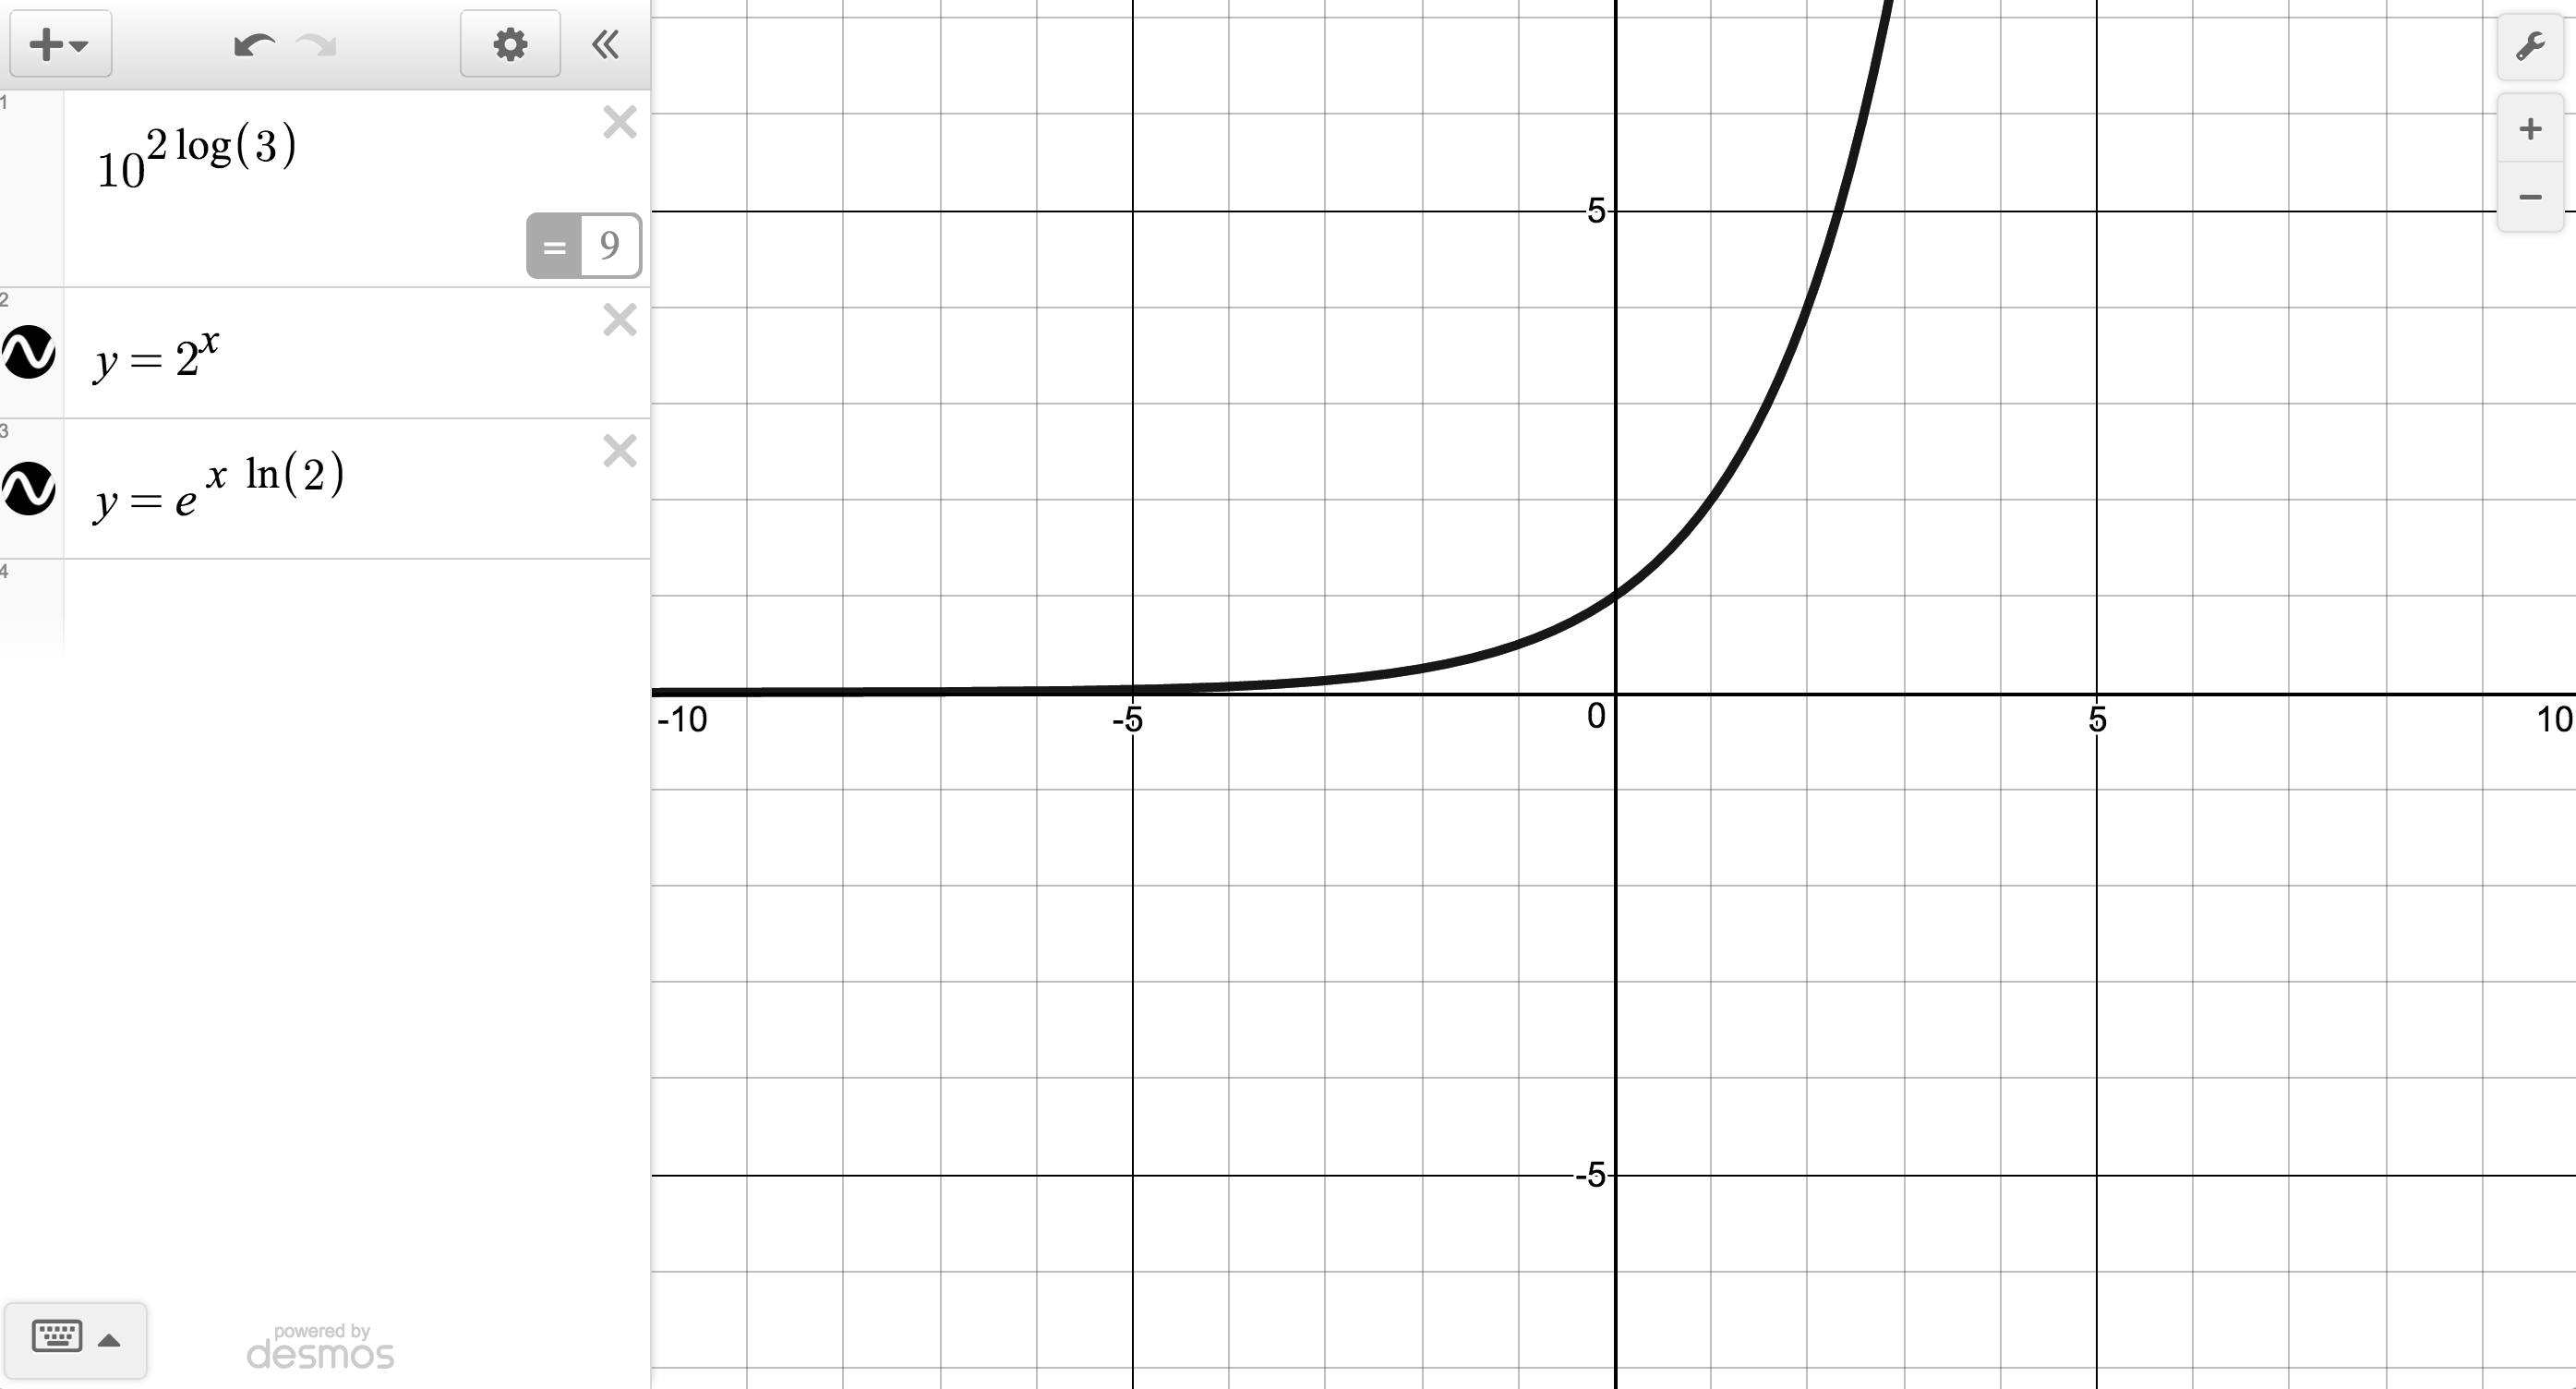
\includegraphics[width=4in]{./PropertiesofLogarithmsGraphics/LogProps01.jpg} 

\end{center}

\item  Applying the change of base with $a=4$ and $b=e$ leads us to write $\log_{4}(5) = \frac{\ln(5)}{\ln(4)}$.  Evaluating this gives the numerical approximation  $\frac{\ln(5)}{\ln(4)} \approx 1.16$. 

\smallskip

To check our answer we know that,  by definition, $\log_{4}(5)$ is the exponent we put on $4$ to get $5$, so a number a little larger than $1$ seems reasonable.

\smallskip

Taking this one step further, we use a graphing utility and find $4^{ \frac{\ln(5)}{\ln(4)}} = 5$, which means if  the machine  is lying to us about the first answer it gave us, at least it is being consistent.

\item  We write $\ln(x) = \log_{e}(x) = \frac{\log(x)}{\log(e)}$.  We graph both $f(x) = \ln(x)$ and $g(x) = \frac{\log(x)}{\log(e)}$ and find both graphs appear to be identical.

\begin{center}

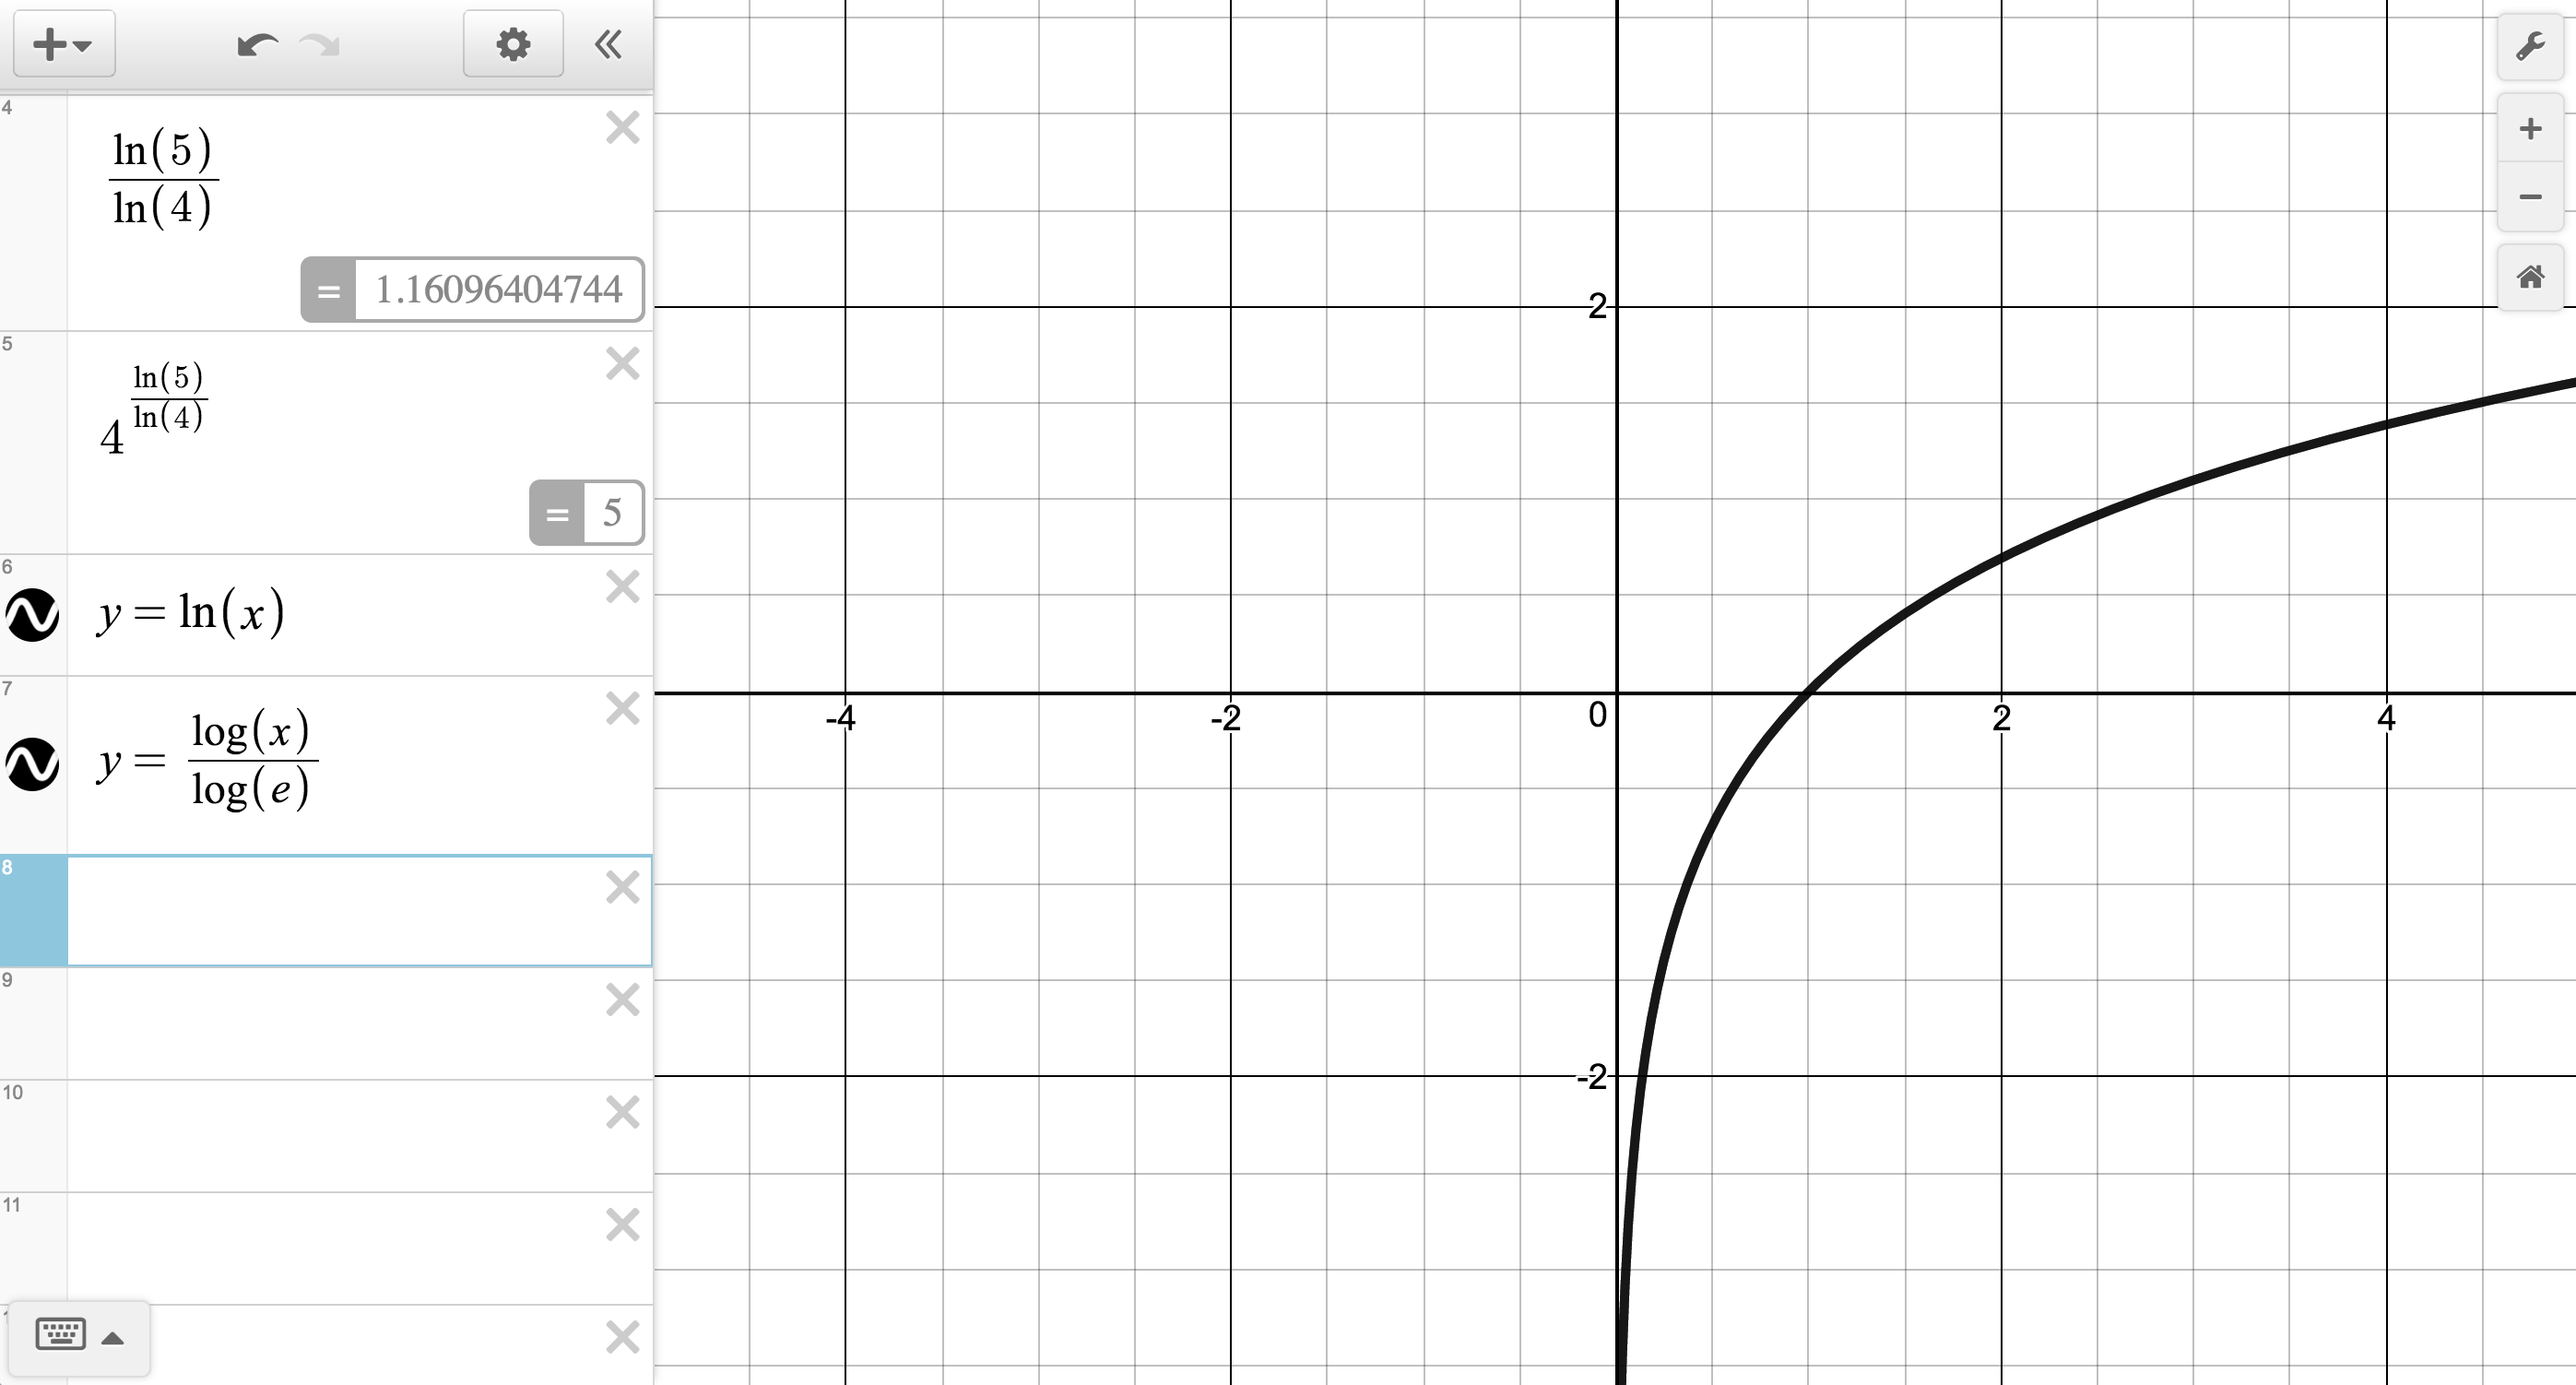
\includegraphics[width=4in]{./PropertiesofLogarithmsGraphics/LogProps02.jpg} 

\end{center}

\end{enumerate}

 \qed

\end{ex}

What Theorem \ref{changeofbase} really tells us is that all exponential and logarithmic functions are just scalings of one another.  Not only does this explain why their graphs have similar shapes, but it also tells us that we could do all of mathematics with a single base,  be it $10$, $0.42$, $\pi$, or $117$. 

\smallskip

As mentioned in Section \ref{ExponentialFunctions}, the `natural' base, base $e$, features prominently in mathematical applications\co{ as we'll see in Section \ref{ExpLogApplications}}.  Hence, we conclude this section by specifying  Theorem \ref{changeofbase} to this case.

\smallskip

\colorbox{ResultColor}{\bbm

\begin{thm}[Conversion to the Natural Base]  \label{allbasee}
Suppose $b>0$, $b \neq 1$. Then

\begin{multicols}{2}

\begin{itemize}

\item $b^{x} = e^{x \ln(b)}$ for all real numbers $x$. \vphantom{$\log_{b}(x) = \dfrac{\ln(x)}{\ln(b)}$}

\item  $\log_{b}(x) = \dfrac{\ln(x)}{\ln(b)}$ for all real numbers $x > 0$.

\end{itemize}

\end{multicols}

\end{thm}

\smallskip

\ebm}



\newpage

\subsection{Exercises}

\label{ExercisesforPropertiesofLogarithms}

In Exercises \ref{expandlogfirst} - \ref{expandloglast}, expand the given logarithm and simplify.  Assume when necessary that all quantities represent positive real numbers.

\begin{multicols}{3}
\begin{enumerate}

\item $\ln(x^{3}y^{2})$ \vphantom{$\log_{2}\left(\dfrac{128}{x^{2} + 4}\right)$} \label{expandlogfirst}
\item $\log_{2}\left(\dfrac{128}{x^{2} + 4}\right)$
\item $\log_{5}\left(\dfrac{z}{25}\right)^{3}$ \vphantom{$\log_{2}\left(\dfrac{128}{x^{2} + 4}\right)$}

\setcounter{HW}{\value{enumi}}
\end{enumerate}
\end{multicols}

\begin{multicols}{3}
\begin{enumerate}
\setcounter{enumi}{\value{HW}}

\item $\log(1.23 \times 10^{37})$ \vphantom{$\ln\left(\dfrac{\sqrt{z}}{xy}\right)$}
\item $\ln\left(\dfrac{\sqrt{z}}{xy}\right)$
\item $\log_{5} \left(x^2 - 25 \right)$ \vphantom{$\ln\left(\dfrac{\sqrt{z}}{xy}\right)$}

\setcounter{HW}{\value{enumi}}
\end{enumerate}
\end{multicols}

\begin{multicols}{3}
\begin{enumerate}
\setcounter{enumi}{\value{HW}}

\item $\log_{\sqrt{2}} \left(4x^3\right)$
\item $\log_{\frac{1}{3}}(9x(y^{3} - 8))$
\item $\log\left(1000x^3y^5\right)$

\setcounter{HW}{\value{enumi}}
\end{enumerate}
\end{multicols}

\begin{multicols}{3}
\begin{enumerate}
\setcounter{enumi}{\value{HW}}

\item $\log_{3} \left(\dfrac{x^2}{81y^4}\right)$
\item $\ln\left(\sqrt[4]{\dfrac{xy}{ez}}\right)$
\item $\log_{6} \left(\dfrac{216}{x^3y}\right)^4$

\setcounter{HW}{\value{enumi}}
\end{enumerate}
\end{multicols}

\begin{multicols}{3}
\begin{enumerate}
\setcounter{enumi}{\value{HW}}

\item $\log\left(\dfrac{100x\sqrt{y}}{\sqrt[3]{10}}\right)$ \vphantom{$\log_{\frac{1}{2}}\left(\dfrac{4\sqrt[3]{x^2}}{y\sqrt{z}}\right)$}
\item $\log_{\frac{1}{2}}\left(\dfrac{4\sqrt[3]{x^2}}{y\sqrt{z}}\right)$
\item $\ln \left(\dfrac{\sqrt[3]{x}}{10 \sqrt{yz}}\right)$ \vphantom{$\log_{\frac{1}{2}}\left(\dfrac{4\sqrt[3]{x^2}}{y\sqrt{z}}\right)$} \label{expandloglast}

\setcounter{HW}{\value{enumi}}
\end{enumerate}
\end{multicols}

In Exercises \ref{combinelogfirst} - \ref{combineloglast}, use the properties of logarithms to write the expression as a single logarithm.

\begin{multicols}{2}
\begin{enumerate}
\setcounter{enumi}{\value{HW}}

\item $4\ln(x) + 2\ln(y)$ \label{combinelogfirst}
\item $\log_{2}(x) + \log_{2}(y) - \log_{2}(z)$

\setcounter{HW}{\value{enumi}}
\end{enumerate}
\end{multicols}

\begin{multicols}{2}
\begin{enumerate}
\setcounter{enumi}{\value{HW}}

\item $\log_{3}(x) - 2 \log_{3}(y)$
\item $\frac{1}{2}\log_{3}(x) - 2\log_{3}(y) - \log_{3}(z)$

\setcounter{HW}{\value{enumi}}
\end{enumerate}
\end{multicols}

\begin{multicols}{2}
\begin{enumerate}
\setcounter{enumi}{\value{HW}}
\item $2 \ln(x) -3 \ln(y) - 4\ln(z)$
\item $\log(x) - \frac{1}{3} \log(z) + \frac{1}{2} \log(y)$

\setcounter{HW}{\value{enumi}}
\end{enumerate}
\end{multicols}

\begin{multicols}{2}
\begin{enumerate}
\setcounter{enumi}{\value{HW}}

\item $-\frac{1}{3} \ln(x) - \frac{1}{3}\ln(y) + \frac{1}{3} \ln(z)$
\item $\log_{5}(x) - 3$

\setcounter{HW}{\value{enumi}}
\end{enumerate}
\end{multicols}

\begin{multicols}{2}
\begin{enumerate}
\setcounter{enumi}{\value{HW}}

\item $3 - \log(x)$
\item $\log_{7}(x) + \log_{7}(x - 3) - 2$

\setcounter{HW}{\value{enumi}}
\end{enumerate}
\end{multicols}

\begin{multicols}{2}
\begin{enumerate}
\setcounter{enumi}{\value{HW}}

\item $\ln(x) + \frac{1}{2}$ 
\item $\log_{2}(x) + \log_{4}(x)$ 

\setcounter{HW}{\value{enumi}}
\end{enumerate}
\end{multicols}

\begin{multicols}{2}
\begin{enumerate}
\setcounter{enumi}{\value{HW}}

\item $\log_{2}(x) + \log_{4}(x-1)$
\item $\log_{2}(x) + \log_{\frac{1}{2}}(x - 1)$ \label{combineloglast}

\setcounter{HW}{\value{enumi}}
\end{enumerate}
\end{multicols}


In Exercises \ref{changeofbasefirst} - \ref{changeofbaselast}, use the appropriate change of base formula to convert the given expression to an expression with the indicated base. 

\begin{multicols}{2}
\begin{enumerate}
\setcounter{enumi}{\value{HW}}

\item $7^{x - 1}$ to base $e$ \label{changeofbasefirst}
\item $\log_{3}(x + 2)$ to base 10

\setcounter{HW}{\value{enumi}}
\end{enumerate}
\end{multicols}

\begin{multicols}{2}
\begin{enumerate}
\setcounter{enumi}{\value{HW}}

\item $\left(\dfrac{2}{3}\right)^{x}$ to base $e$
\item $\log(x^{2} + 1)$ to base $e$ \vphantom{$\left(\dfrac{2}{3}\right)^{x}$}\label{changeofbaselast}

\setcounter{HW}{\value{enumi}}
\end{enumerate}
\end{multicols}

\newpage

In Exercises \ref{changeofbaseapproxfirst} - \ref{changeofbaseapproxlast}, use the appropriate change of base formula to approximate the logarithm.

\begin{multicols}{3}
\begin{enumerate}
\setcounter{enumi}{\value{HW}}

\item $\log_{3}(12)$ \label{changeofbaseapproxfirst}
\item $\log_{5}(80)$
\item $\log_{6}(72)$

\setcounter{HW}{\value{enumi}}
\end{enumerate}
\end{multicols}

\begin{multicols}{3}
\begin{enumerate}
\setcounter{enumi}{\value{HW}}

\item $\log_{4}\left(\dfrac{1}{10}\right)$
\item $\log_{\frac{3}{5}}(1000)$ \vphantom{$\log_{4}\left(\dfrac{1}{10}\right)$}
\item $\log_{\frac{2}{3}}(50)$ \vphantom{$\log_{4}\left(\dfrac{1}{10}\right)$} \label{changeofbaseapproxlast}

\setcounter{HW}{\value{enumi}}
\end{enumerate}
\end{multicols}

\begin{enumerate}
\setcounter{enumi}{\value{HW}}

\item \label{morethanoneforlogexercise} In Example \ref{intrologex} number \ref{findformulaforlogexample} in Section \ref{LogarithmicFunctions}, we obtained the solution  $F(x) = \log_{2}(-x+4)-3$ as one formula for the given graph by making a simplifying assumption that $b = -1$.  This exercises explores if there are any other solutions for different choices of $b$.

\begin{enumerate}

\item  Show  $G(x) =\log_{2}(-2x+8) - 4$ also fits the data for the given graph.

\item  Use properties of logarithms to show $G(x) = \log_{2}(-2x+8) -4  = \log_{2}(-x+4)-3 = F(x)$.

\item  With help from your classmates, find solutions to Example \ref{intrologex} number \ref{findformulaforlogexample} in Section \ref{LogarithmicFunctions} by assuming $b = -4$ and $b = -8$.  In each case, use properties of logarithms to show the solutions reduce to $F(x) = \log_{2}(-x+4)-3$.

\item  Using properties of logarithms and the fact that the range of $\log_{2}(x)$ is all real numbers, show that any function of the form $f(x) = a \log_{2}(bx-h) + k$ where $a \neq 0$ can be rewritten as: 

\[ f(x) = a \left( \log_{2}(bx-h) +  \frac{k}{a}\right) = a ( \log_{2}(bx -h) + \log_{2}(p)) = a \log_{2}(p(bx-h)) = a \log_{2}(pbx - ph),\]

where $\frac{k}{a} = \log_{2}(p)$ for some positive real number $p$. Relabeling, we get every function of the form $f(x) = a \log_{2}(bx-h) + k$ with four parameters ($a$, $b$, $h$, and $k$) can be rewritten as $f(x) = a \log_{2}(Bx - H)$, a formula with just three parameters: $a$, $B$, and $H$.

\smallskip

Show \textit{every} solution to Example \ref{intrologex} number \ref{findformulaforlogexample} in Section \ref{LogarithmicFunctions} can be written in the form  $f(x) = \log_{2}\left( -\frac{1}{8}  x + \frac{1}{2} \right)$ and that, in particular,  $F(x) = \log_{2}(-x+4) -3 = \log_{2}\left( -\frac{1}{8}  x + \frac{1}{2} \right) = f(x)$.  Hence, there is really just one solution to Example \ref{intrologex} number \ref{findformulaforlogexample} in Section \ref{LogarithmicFunctions}.

\end{enumerate}   

\item \label{HendersonHasselbalch} \index{Henderson-Hasselbalch Equation} The Henderson-Hasselbalch Equation:  Suppose $HA$ represents a weak acid. Then we have a reversible chemical reaction 
\[HA \rightleftharpoons H^{+} + A^{-}.\]  
The acid disassociation constant, $K_{a}$, is given by 
\[K_{a} = \frac{[H^{+}][A^{-}]}{[HA]} = [H^{+}]\frac{[A^{-}]}{[HA]},\]
where the square brackets denote the concentrations just as they did in Exercise \ref{pHexercise} in Section \ref{LogarithmicFunctions}.  The symbol p$K_{a}$ is defined similarly to pH in that p$K_{a} = -\log(K_{a})$.  Using the definition of pH from Exercise \ref{pHexercise} and the properties of logarithms, derive the Henderson-Hasselbalch Equation:

\[\mbox{pH} = \mbox{p}K_{a} + \log\dfrac{[A^{-}]}{[HA]}\]

\item Compare and contrast the graphs of $y = \ln(x^{2})$ and $y = 2\ln(x)$.

\item Prove the Quotient Rule and Power Rule for Logarithms.

\item Give numerical examples to show that, in general,

\begin{multicols}{2}
\begin{enumerate}

\item $\log_{b}(x + y) \neq \log_{b}(x) + \log_{b}(y)$
\item $\log_{b}(x - y) \neq \log_{b}(x) - \log_{b}(y)$
\setcounter{HWindent}{\value{enumii}}
\end{enumerate}
\end{multicols}

\begin{enumerate}
\setcounter{enumii}{\value{HWindent}}

\item $\log_{b}\left(\dfrac{x}{y}\right) \neq \dfrac{\log_{b}(x)}{\log_{b}(y)}$

\end{enumerate}

\item Research the history of logarithms including the origin of the word `logarithm' itself.  Why is the abbreviation of natural log `ln' and not `nl'?

\item There is a scene in the movie `Apollo 13' in which several people at Mission Control use slide rules to verify a computation.  Was that scene accurate?  Look for other pop culture references to logarithms and slide rules.


\setcounter{HW}{\value{enumi}}
\end{enumerate}


\newpage

\subsection{Answers}


\begin{multicols}{2}
\begin{enumerate}

\item $3\ln(x) + 2\ln(y)$
\item $7 - \log_{2}(x^{2} + 4)$

\setcounter{HW}{\value{enumi}}
\end{enumerate}
\end{multicols}

\begin{multicols}{2}
\begin{enumerate}
\setcounter{enumi}{\value{HW}}


\item $3\log_{5}(z) - 6$
\item $\log(1.23) + 37$

\setcounter{HW}{\value{enumi}}
\end{enumerate}
\end{multicols}

\begin{multicols}{2}
\begin{enumerate}
\setcounter{enumi}{\value{HW}}

\item $\frac{1}{2}\ln(z) - \ln(x) - \ln(y)$
\item  $\log_{5}(x-5) + \log_{5}(x+5)$

\setcounter{HW}{\value{enumi}}
\end{enumerate}
\end{multicols}

\begin{multicols}{2}
\begin{enumerate}
\setcounter{enumi}{\value{HW}}

\item  $3\log_{\sqrt{2}}(x) + 4$
\item \small$-2 + \log_{\frac{1}{3}}(x) + \log_{\frac{1}{3}}(y - 2) + \log_{\frac{1}{3}}(y^{2} + 2y + 4)$\normalsize

\setcounter{HW}{\value{enumi}}
\end{enumerate}
\end{multicols}

\begin{multicols}{2}
\begin{enumerate}
\setcounter{enumi}{\value{HW}}

\item $3 + 3\log(x) + 5 \log(y)$
\item $2\log_{3}(x) - 4 - 4\log_{3}(y)$

\setcounter{HW}{\value{enumi}}
\end{enumerate}
\end{multicols}

\begin{multicols}{2}
\begin{enumerate}
\setcounter{enumi}{\value{HW}}

\item $\frac{1}{4} \ln(x) + \frac{1}{4} \ln(y) - \frac{1}{4} - \frac{1}{4} \ln(z)$
\item $12-12\log_{6}(x) - 4\log_{6}(y)$

\setcounter{HW}{\value{enumi}}
\end{enumerate}
\end{multicols}

\begin{multicols}{2}
\begin{enumerate}
\setcounter{enumi}{\value{HW}}

\item $\frac{5}{3}+\log(x)+\frac{1}{2}\log(y)$
\item $-2+\frac{2}{3}\log_{\frac{1}{2}}(x)-\log_{\frac{1}{2}}(y)-\frac{1}{2}\log_{\frac{1}{2}}(z)$

\setcounter{HW}{\value{enumi}}
\end{enumerate}
\end{multicols}

\begin{multicols}{2}
\begin{enumerate}
\setcounter{enumi}{\value{HW}}

\item $\frac{1}{3} \ln(x) - \ln(10) - \frac{1}{2}\ln(y)-\frac{1}{2}\ln(z)$
\item $\ln(x^{4}y^{2})$
\setcounter{HW}{\value{enumi}}
\end{enumerate}
\end{multicols}

\begin{multicols}{3}
\begin{enumerate}
\setcounter{enumi}{\value{HW}}

\item $\log_{2}\left(\frac{xy}{z}\right)$
\item $\log_{3} \left( \frac{x}{y^2} \right)$
\item $\log_{3}\left(\frac{\sqrt{x}}{y^{2}z}\right)$

\setcounter{HW}{\value{enumi}}
\end{enumerate}
\end{multicols}

\begin{multicols}{3}
\begin{enumerate}
\setcounter{enumi}{\value{HW}}


\item $\ln\left( \frac{x^2}{y^3z^4} \right)$
\item $\log\left(\frac{x \sqrt{y}}{\sqrt[3]{z}}  \right)$
\item $\ln\left(\sqrt[3]{\frac{z}{xy}}   \right)$

\setcounter{HW}{\value{enumi}}
\end{enumerate}
\end{multicols}

\begin{multicols}{3}
\begin{enumerate}
\setcounter{enumi}{\value{HW}}

\item $\log_{5}\left(\frac{x}{125}\right)$
\item $\log\left(\frac{1000}{x}\right)$
\item $\log_{7}\left(\frac{x(x - 3)}{49}\right)$

\setcounter{HW}{\value{enumi}}
\end{enumerate}
\end{multicols}

\begin{multicols}{3}
\begin{enumerate}
\setcounter{enumi}{\value{HW}}

\item $\ln \left(x \sqrt{e} \right)$
\item $\log_{2}\left(x^{3/2}\right)$
\item $\log_{2}\left(x \sqrt{x-1}\right)$


\setcounter{HW}{\value{enumi}}
\end{enumerate}
\end{multicols}


\begin{multicols}{3}
\begin{enumerate}
\setcounter{enumi}{\value{HW}}
\item $\vphantom{\frac{\log(x + 2)}{\log(3)}}\log_{2}\left(\frac{x}{x - 1}\right)$ 
\item $\vphantom{\frac{\log(x + 2)}{\log(3)}}7^{x - 1} = e^{(x - 1)\ln(7)}$
\item $\log_{3}(x + 2) = \frac{\log(x + 2)}{\log(3)}$


\setcounter{HW}{\value{enumi}}
\end{enumerate}
\end{multicols}


\begin{multicols}{2}
\begin{enumerate}
\setcounter{enumi}{\value{HW}}

\item $\left(\frac{2}{3}\right)^{x} = e^{x\ln(\frac{2}{3})}$
\item $\log(x^{2} + 1) = \frac{\ln(x^{2} + 1)}{\ln(10)}$

\setcounter{HW}{\value{enumi}}
\end{enumerate}
\end{multicols}

\begin{multicols}{2}
\begin{enumerate}
\setcounter{enumi}{\value{HW}}

\item $\log_{3}(12) \approx 2.26186$
\item $\log_{5}(80) \approx 2.72271$

\setcounter{HW}{\value{enumi}}
\end{enumerate}
\end{multicols}

\begin{multicols}{2}
\begin{enumerate}
\setcounter{enumi}{\value{HW}}

\item $\log_{6}(72) \approx 2.38685$
\item $\log_{4}\left(\frac{1}{10}\right) \approx -1.66096$

\setcounter{HW}{\value{enumi}}
\end{enumerate}
\end{multicols}

\begin{multicols}{2}
\begin{enumerate}
\setcounter{enumi}{\value{HW}}
\item $\log_{\frac{3}{5}}(1000) \approx -13.52273$
\item $\log_{\frac{2}{3}}(50) \approx -9.64824$

\setcounter{HW}{\value{enumi}}
\end{enumerate}
\end{multicols}


\closegraphsfile


\newpage

\section{Equations involving Exponential Functions}

\mfpicnumber{1}

\opengraphsfile{ExponentialEquationsandInequalities}

\setcounter{footnote}{0}

\label{ExponentialEquationsandInequalities}

In this section we will develop techniques for solving equations involving exponential functions.  Consider the equation $2^{x} = 128$.  After a moment's calculation, we find $128 = 2^{7}$, so we have $2^{x} = 2^{7}$.  The one-to-one property of exponential functions, detailed in Theorem \ref{explogsonetoone}, tells us that $2^{x} = 2^{7}$ if and only if $x=7$.  This means that not only is $x=7$ a solution to $2^{x} = 2^{7}$, it is the \textit{only} solution.  

\smallskip

Now suppose we change the problem ever so slightly to $2^{x} = 129$.  We could use one of the inverse properties of exponentials and logarithms listed in Theorem \ref{invpropslogs} to write $129 = 2^{\log_{2}(129)}$.  We'd then have $2^{x} = 2^{\log_{2}(129)}$, which means our solution is $x = \log_{2}(129)$. 

\smallskip

After all, the definition of $\log_{2}(129)$ is `the exponent we put on $2$ to get $129$.' Indeed we could have obtained this solution directly by rewriting the equation $2^{x} = 129$ in its logarithmic form $\log_{2}(129) = x$.  Either way, in order to get a reasonable decimal approximation to this number, we'd use the change of base formula, Theorem \ref{changeofbase}, to give us something more calculator friendly.  Typically this means we convert our answer to base 10 or base $e$, and we choose the latter: $\log_{2}(129) = \frac{\ln(129)}{\ln(2)} \approx 7.011$.  

\smallskip

Still another way to obtain this answer is to `take the natural log' of both sides of the equation. Since $f(x) = \ln(x)$ is a \textit{function}, as long as two quantities are equal, their natural logs are equal.\footnote{This is also the `if' part of the statement $\log_{b}(u) = \log_{b}(w)$ if and only if $u=w$ in Theorem \ref{explogsonetoone}.} 

\smallskip

We then use the Power Rule to write the exponent $x$ as a factor then divide both sides by the constant $\ln(2)$ to obtain our answer.\footnote{ Please resist the temptation to divide both sides by `$\ln$' instead of $\ln(2)$.   Just like it wouldn't make sense to divide both sides by the square root symbol `$\sqrt{\vphantom{2} \,}$' when solving $x \sqrt{2} = 5$, it makes no sense to divide by `$\ln$'.}

\[ \begin{array}{rclr}
2^{x} & = & 129 & \\
\ln\left(2^{x}\right) & = & \ln(129) & \mbox{Take the natural log of both sides.} \\
x \ln(2) & = & \ln(129) & \mbox{Power Rule} \\ [4pt]
x & = &\dfrac{\ln(129)}{\ln(2)} & \\
\end{array}\]

We summarize our two strategies for solving equations featuring exponential functions below.

\smallskip

\colorbox{ResultColor}{\bbm

\centerline{\textbf{Steps for Solving an Equation involving Exponential Functions}} \index{exponential function ! solving equations with}

\begin{enumerate}

\item  Isolate the exponential function.

\item  

\begin{enumerate}

\item  If convenient, express both sides with a common base and equate the exponents.

\item  Otherwise, take the natural log of both sides of the equation and use the Power Rule.


\end{enumerate}


\end{enumerate}

\ebm}

\smallskip


\begin{ex}  \label{expeqnsex1} Solve the following equations.  Check your answer using a graphing utility.

\begin{multicols}{3}
\begin{enumerate}

\item  $2^{3x} = 16^{1-x}$

\item  $2000 = 1000 \cdot 3^{-0.1 t}$ 

\item  $9 \cdot 3^{x} = 7^{2x}$

\setcounter{HW}{\value{enumi}}
\end{enumerate}
\end{multicols}

\begin{multicols}{3}
\begin{enumerate}
\setcounter{enumi}{\value{HW}}

\item  $75 = \frac{100}{1 + 3e^{-2t}}$

\item  $25^{x} = 5^{x} + 6$

\item  $\frac{e^{x} - e^{-x}}{2} = 5$

\end{enumerate}
\end{multicols}

\newpage

{\bf Solution.}

\begin{enumerate}

\item  Since $16$ is a power of $2$, we can rewrite  $2^{3x} =  16^{1-x}$ as $2^{3x} = \left(2^4\right)^{1-x}$.  Using properties of exponents, we get $2^{3x} = 2^{4(1-x)}$.  

\smallskip

Using the one-to-one property of exponential functions, we get $3x = 4(1-x)$ which gives $x=\frac{4}{7}$. 

\smallskip

Graphing $f(x) = 2^{3x}$ and $g(x) = 16^{1-x}$ and see that they intersect at $x \approx 0.571  \approx \frac{4}{7}$.

\item  We begin solving $2000 = 1000 \cdot 3^{-0.1 t}$  by dividing both sides by $1000$ to isolate the exponential which yields $3^{-0.1t} = 2$.  

\smallskip

Since it is inconvenient to write $2$ as a power of $3$, we use the natural log to get $\ln\left(3^{-0.1t}\right) = \ln(2)$.  

\smallskip

Using the Power Rule, we get $-0.1 t \ln(3) = \ln(2)$, so we divide both sides by $-0.1 \ln(3)$  and obtain $t = -\frac{\ln(2)}{0.1 \ln(3)} = -\frac{10\ln(2)}{\ln(3)}$.  

\smallskip

We see the graphs of  $f(x) = 2000$ and $g(x) =  1000 \cdot 3^{-0.1 x}$ intersect at $x \approx -6.309 \approx -\frac{10\ln(2)}{\ln(3)} $.

\begin{center}

\begin{tabular}{cc}

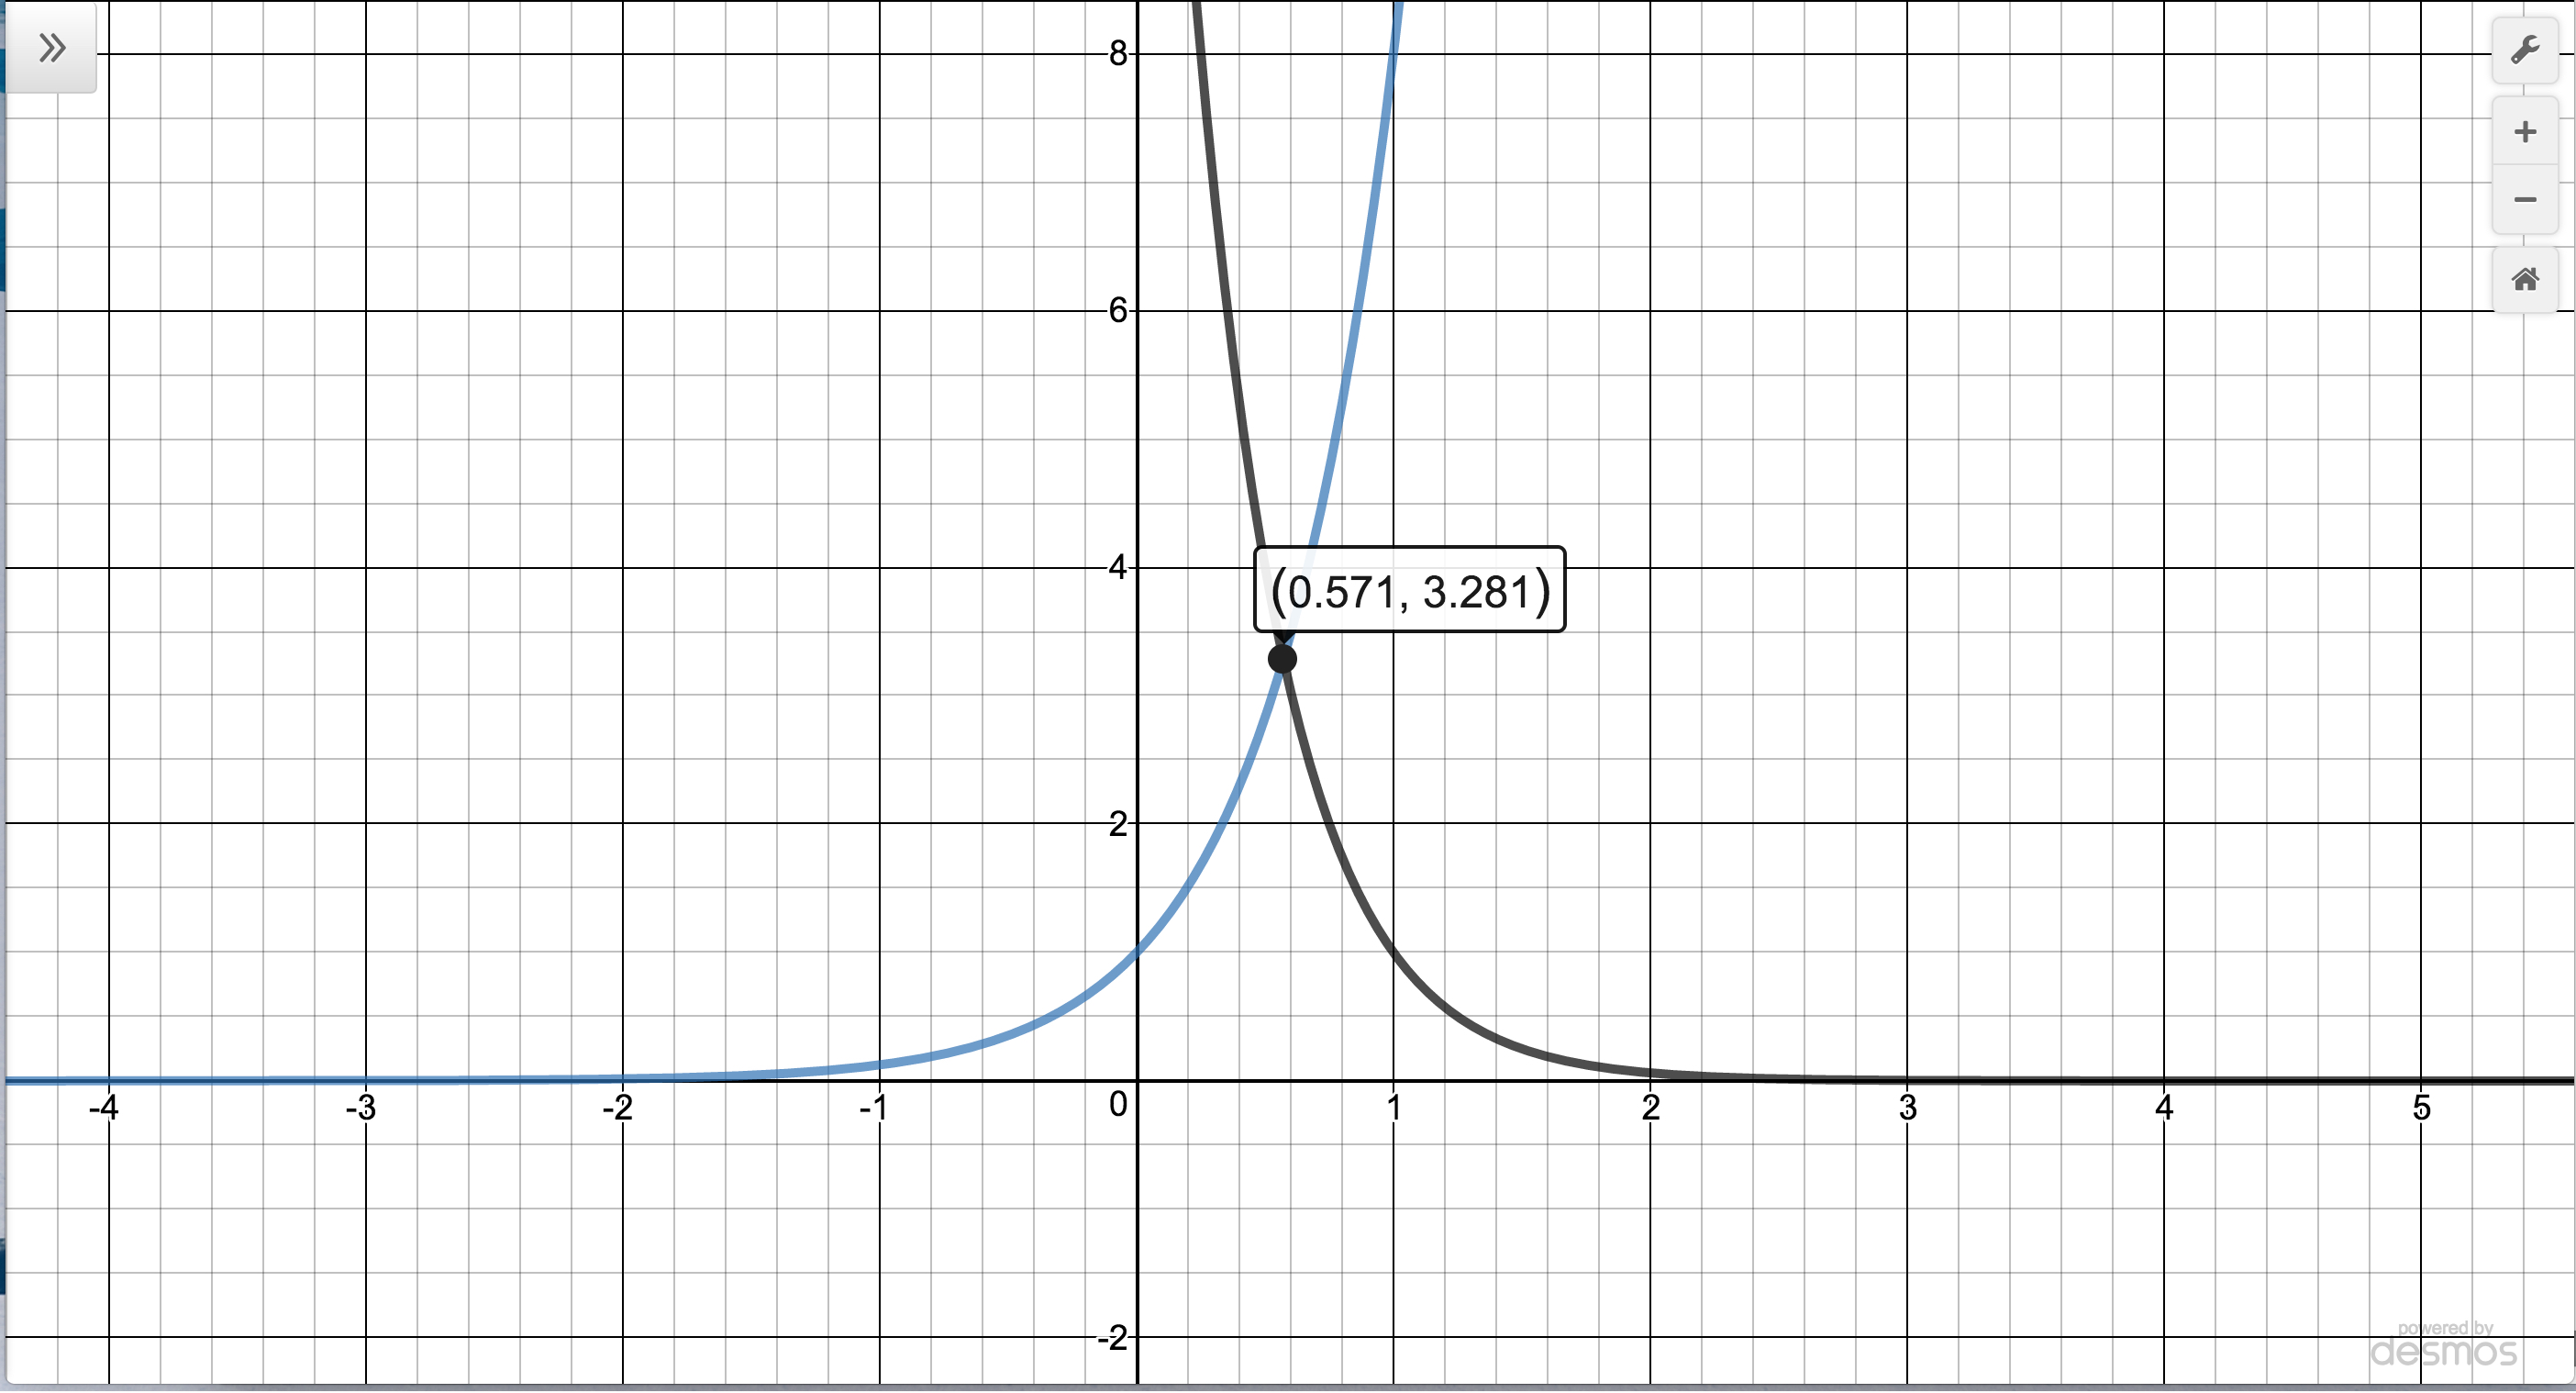
\includegraphics[width=3in]{./ExponentialEquationsandInequalitiesGraphics/ExpEqnEx01.jpg} &

 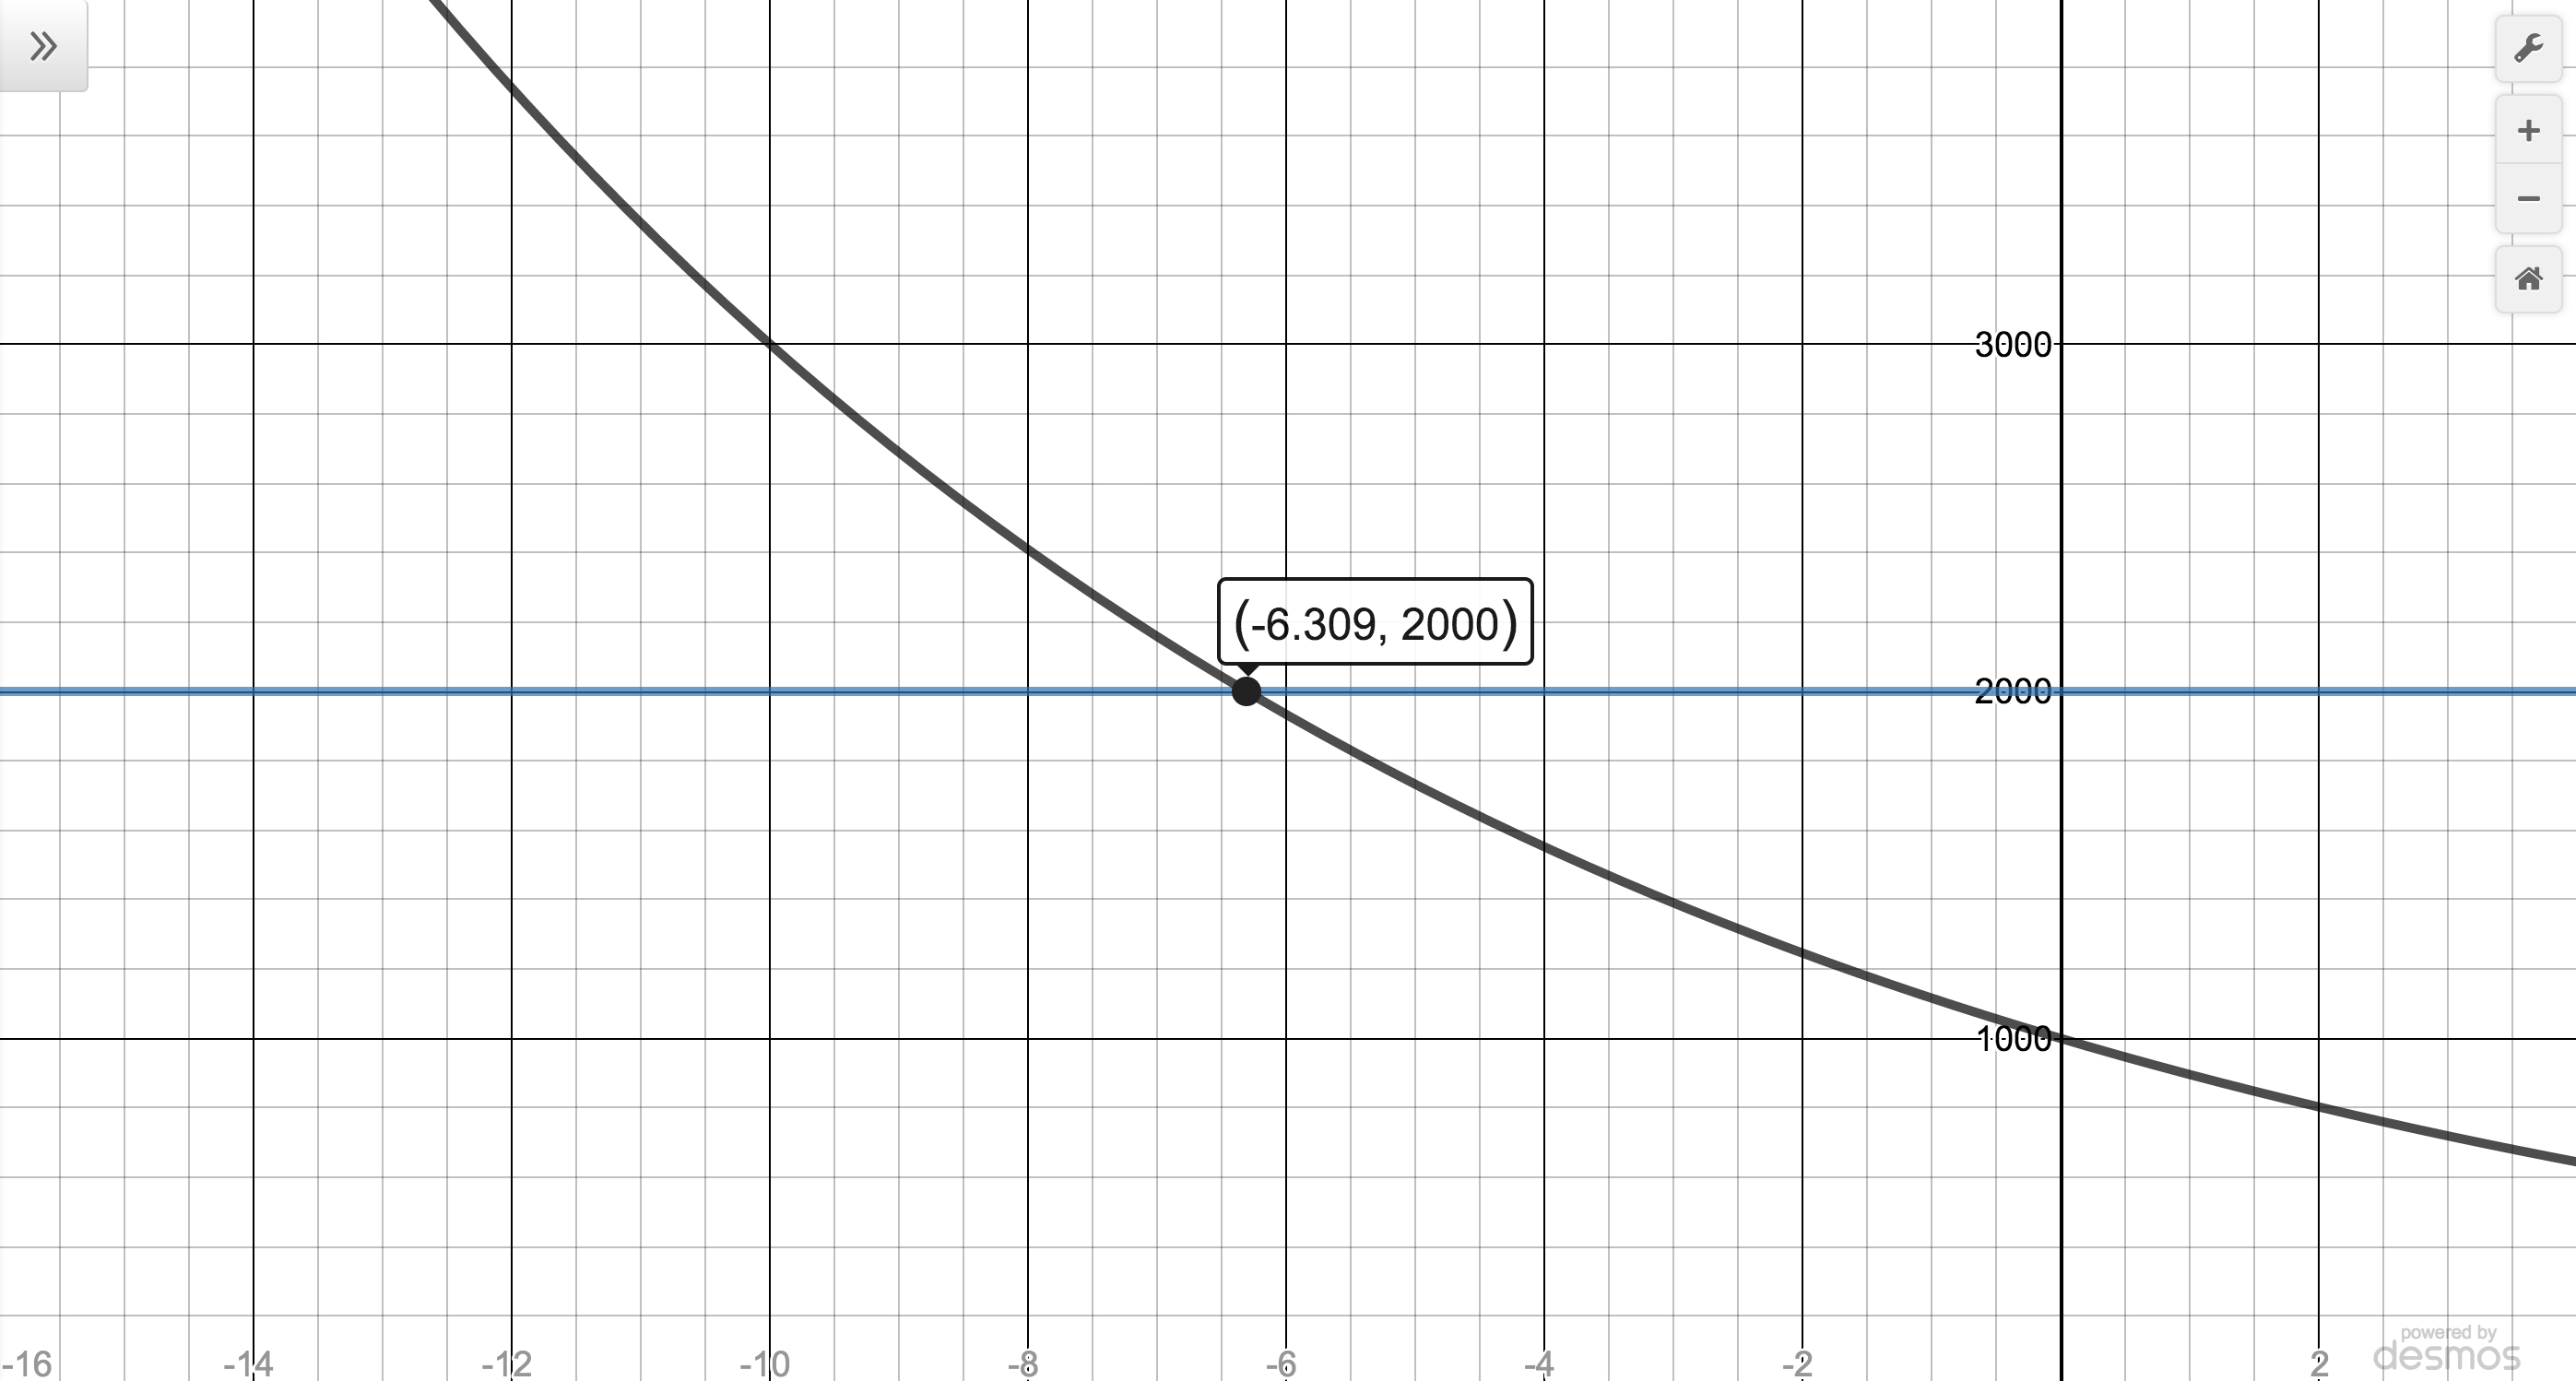
\includegraphics[width=3in]{./ExponentialEquationsandInequalitiesGraphics/ExpEqnEx02.jpg} \\

Checking $2^{3x} = 16^{1-x}$ 
 
 &
 
 Checking $2000 = 1000 \cdot 3^{-0.1 t}$
 
\end{tabular}

\end{center}

\item  We first note that we can rewrite the equation $9 \cdot 3^{x} = 7^{2x}$ as $3^2 \cdot 3^x = 7^{2x}$ to obtain $3^{x+2} = 7^{2x}$. 

\smallskip

Since it is not convenient to express both sides as a power of $3$ (or $7$ for that matter) we use the natural log:  $\ln\left(3^{x+2}\right) = \ln\left(7^{2x}\right)$.  

\smallskip

The power rule gives $(x+2) \ln(3) = 2x \ln(7)$.  Even though this equation appears very complicated, keep in mind that $\ln(3)$ and $\ln(7)$ are just constants.  

\smallskip

The equation $(x+2) \ln(3) = 2x \ln(7)$ is actually a linear equation (do you see why?) and as such we gather all of the terms with $x$ on one side, and the constants on the other.  We then divide both sides by the coefficient of $x$, which we obtain by factoring.

\[ \begin{array}{rclr}
(x+2) \ln(3) & = & 2x \ln(7) & \\

x \ln(3) + 2 \ln(3) & = & 2x \ln(7) & \\
2 \ln(3) & = & 2x \ln(7) - x \ln(3) & \\
2 \ln(3) & = & x (2 \ln(7) - \ln(3)) & \mbox{Factor.}\\
x & = & \frac{2 \ln(3)}{2\ln(7) - \ln(3)} & \\ [4pt]
\end{array}\]

We see the graphs of $f(x) = 9 \cdot 3^{x}$ and $g(x) = 7^{2x}$ intersect at $x  \approx 0.787 \approx  \frac{2 \ln(3)}{2\ln(7) - \ln(3)}$.

\item  Our objective in solving  $75 = \frac{100}{1 + 3e^{-2t}}$ is to first isolate the exponential.  

\smallskip

To that end, we clear denominators and get $75\left(1 + 3e^{-2t}\right) = 100$, or $75 + 225e^{-2t} =100$.   We get  $225e^{-2t} = 25$, so finally, $e^{-2t} = \frac{1}{9}$.    

\smallskip

Taking the natural log of both sides gives $\ln\left(e^{-2t}\right) = \ln\left( \frac{1}{9} \right)$.  Since natural log is log base $e$, $\ln\left(e^{-2t}\right) = -2t$.  Likewise, we use the Power Rule to rewrite $\ln\left( \frac{1}{9} \right) = -\ln(9)$.  

\smallskip

Putting these two steps together, we simplify $\ln\left(e^{-2t}\right) = \ln\left( \frac{1}{9} \right)$ to   $-2t = -\ln(9)$.  We arrive at our solution, $t = \frac{\ln(9)}{2}$ which simplifies to $t = \ln(3)$. (Can you explain why?)  

\smallskip

 To check, we see the graphs of  $f(x) = 75$ and $g(x) = \frac{100}{1 + 3e^{-2x}}$,  intersect at $x \approx 1.099 \approx \ln(3)$.

\begin{center}

\begin{tabular}{cc}

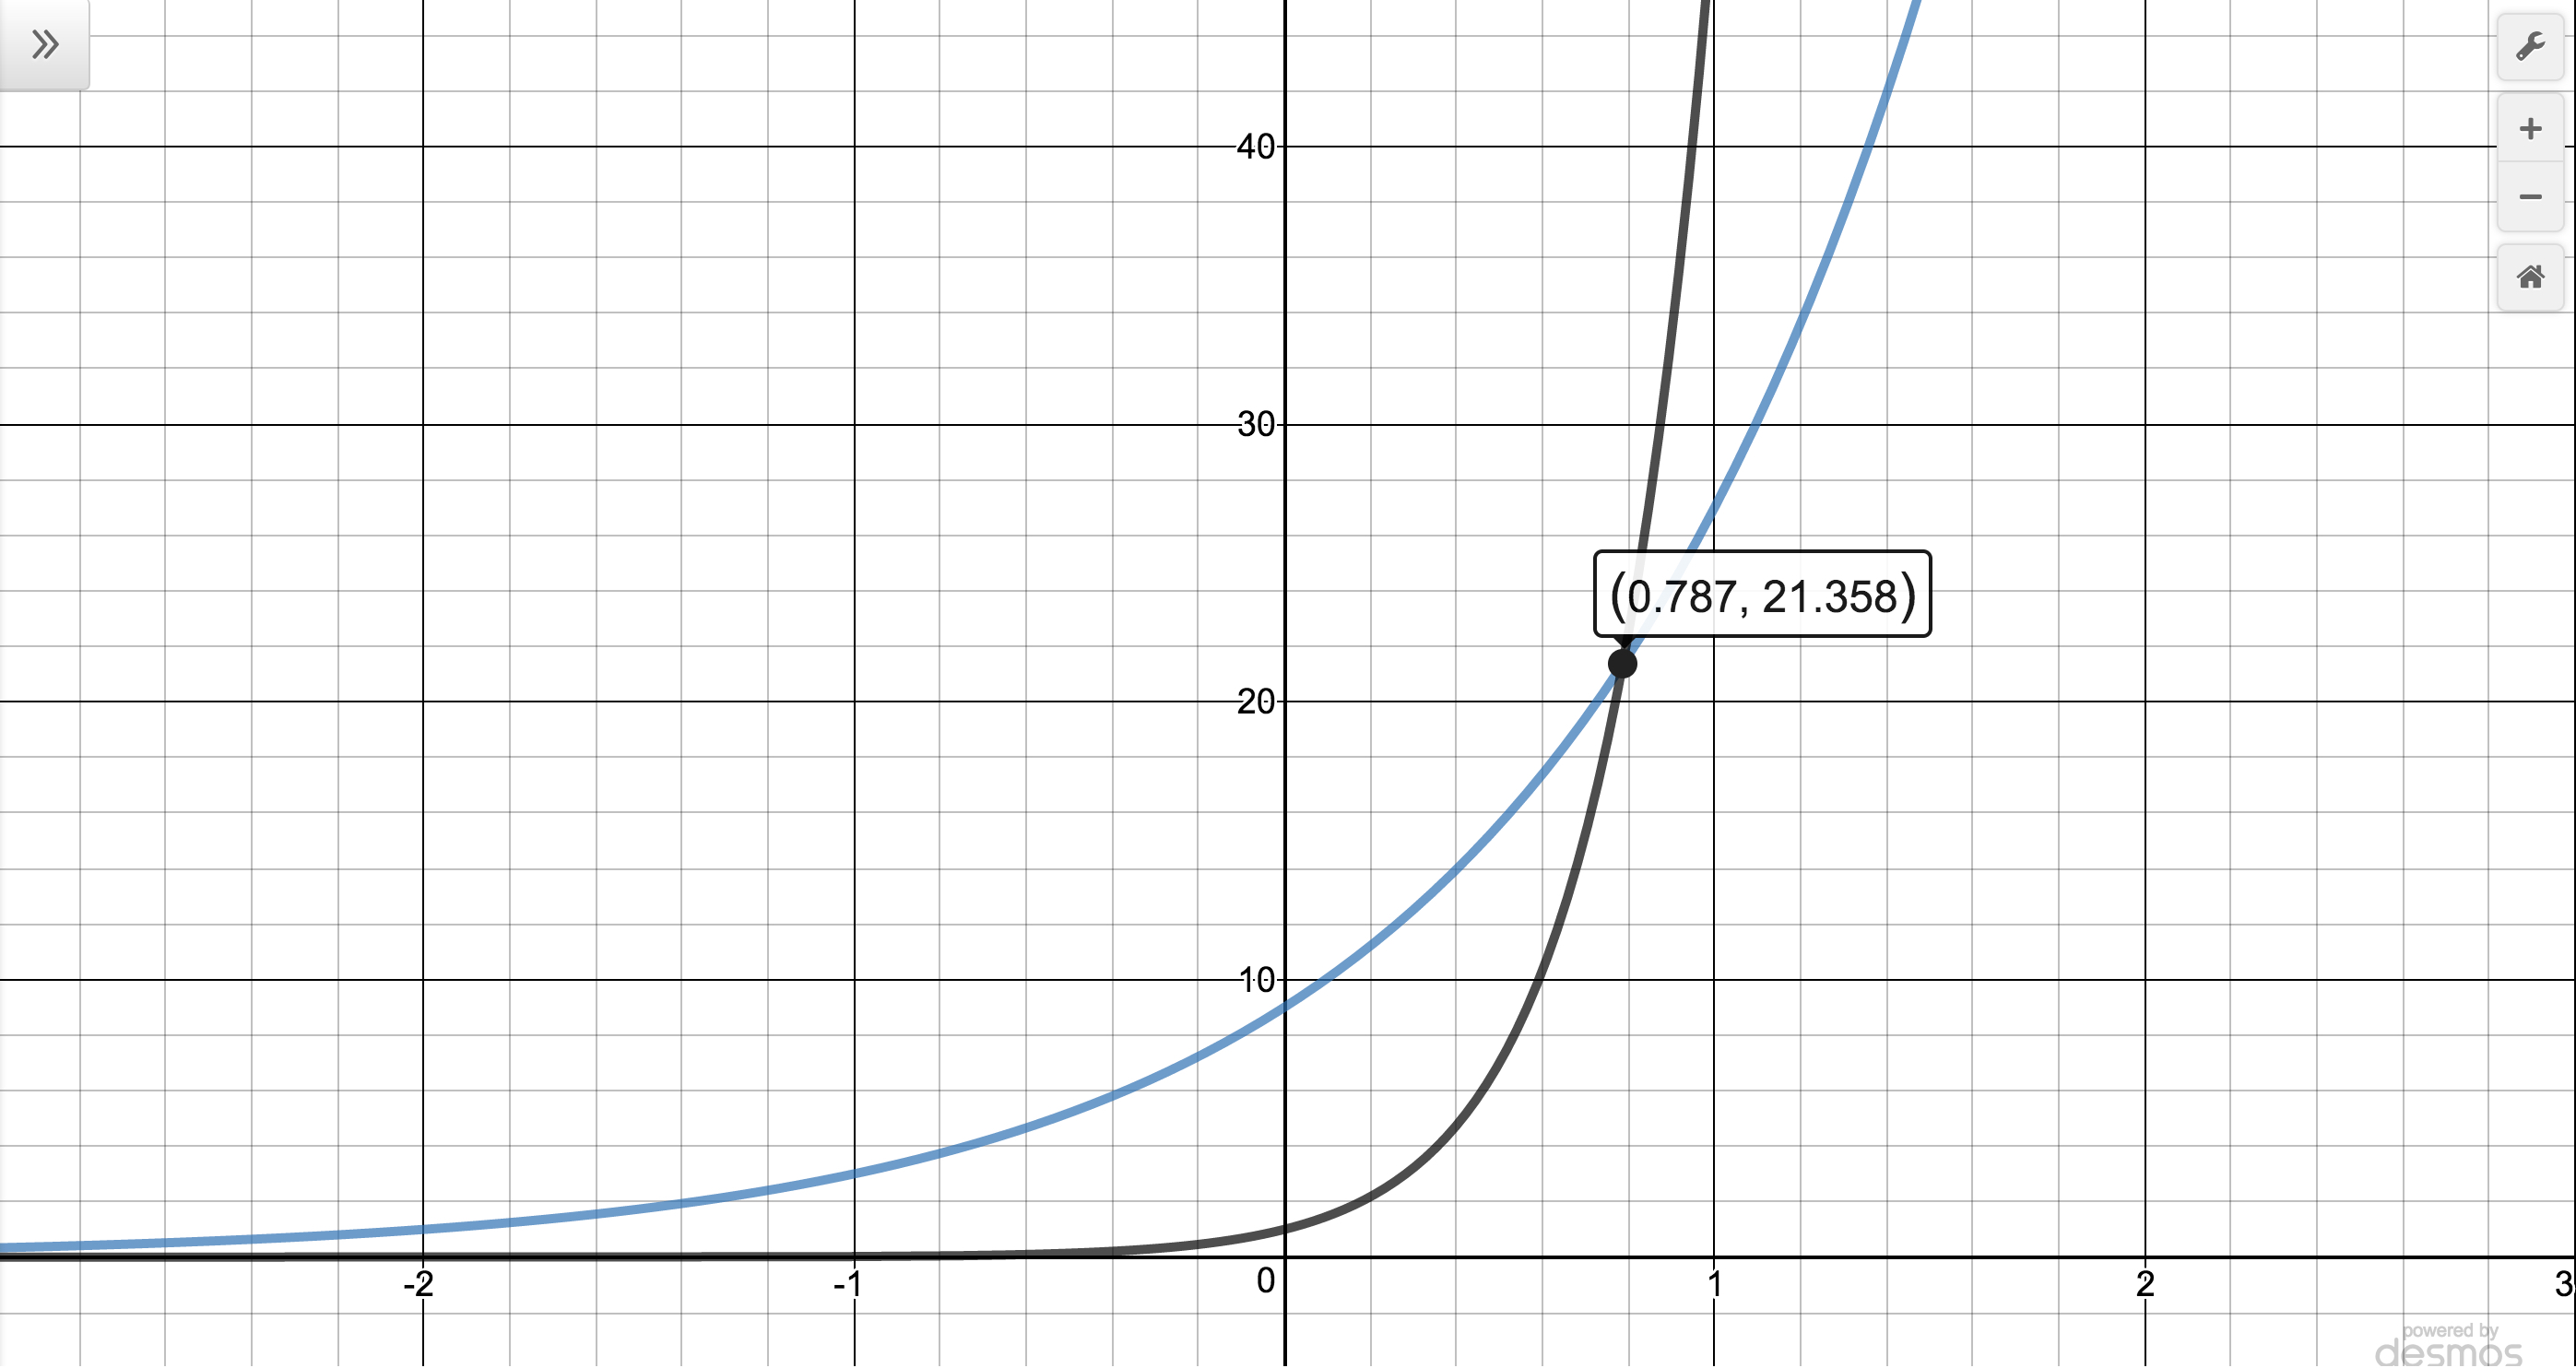
\includegraphics[width=3in]{./ExponentialEquationsandInequalitiesGraphics/ExpEqnEx03.jpg} &

 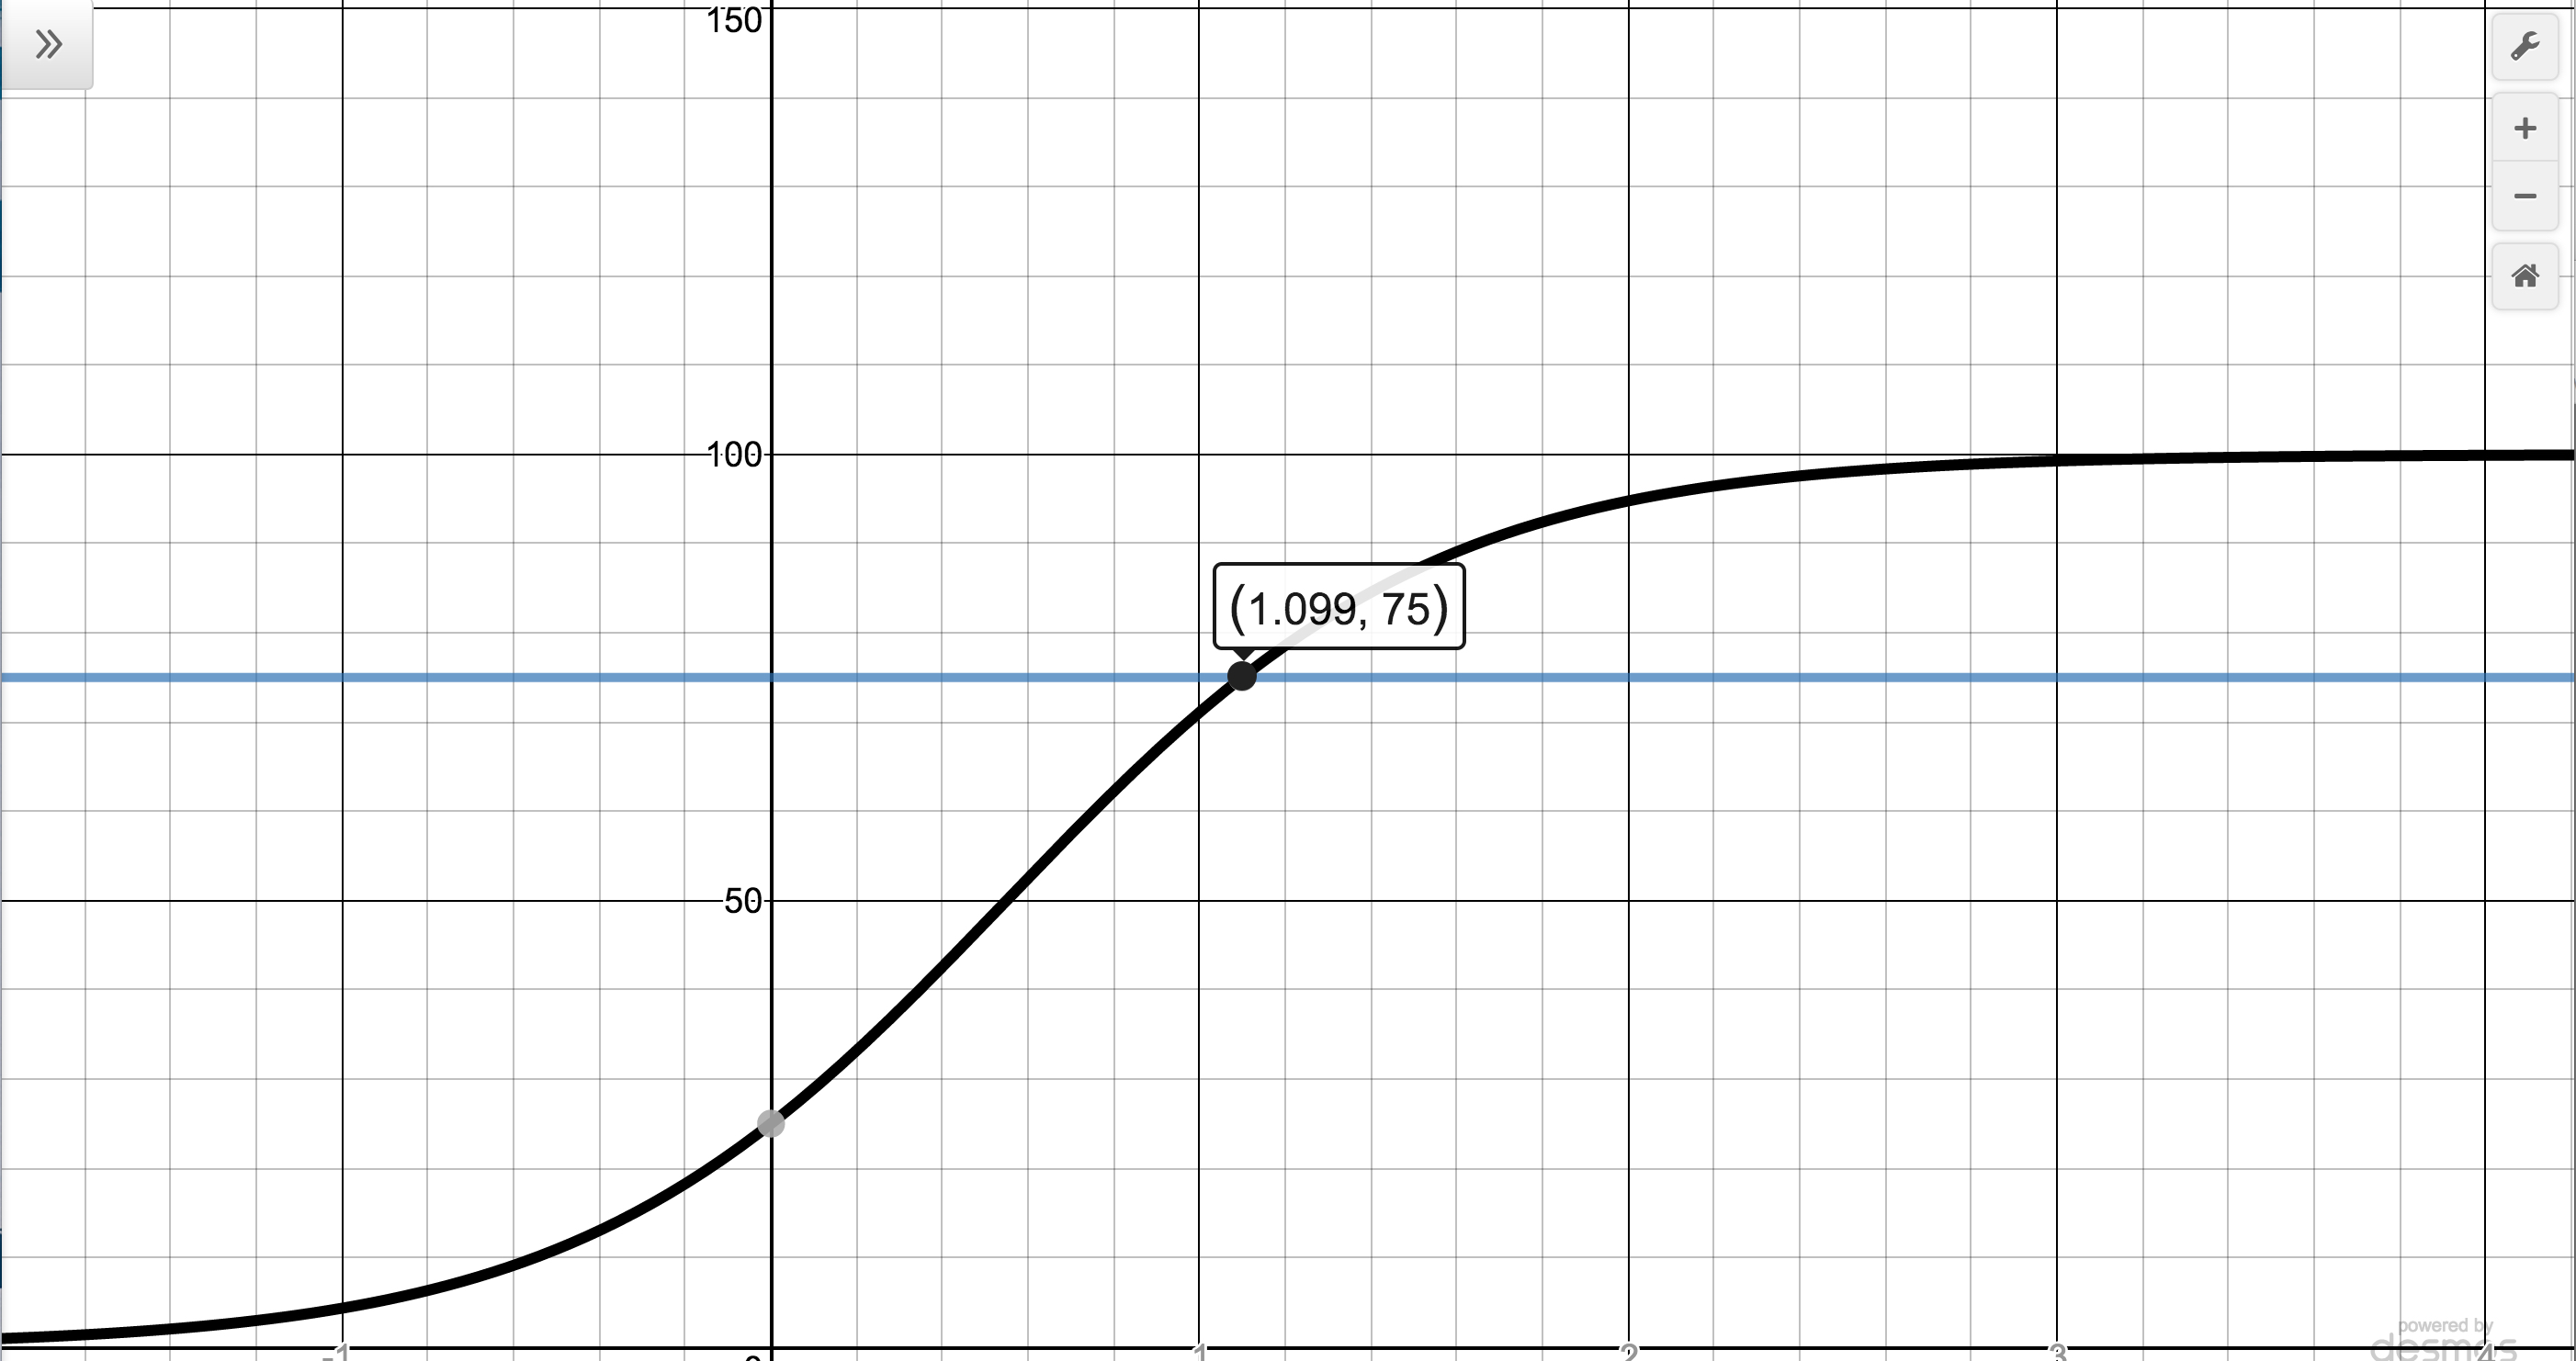
\includegraphics[width=3in]{./ExponentialEquationsandInequalitiesGraphics/ExpEqnEx04.jpg} \\

Checking $9 \cdot 3^{x} = 7^{2x}$ 
 
 &
 
 Checking $75 = \frac{100}{1 + 3e^{-2t}}$
 
\end{tabular}

\end{center}

\item  We start solving $25^{x} = 5^{x} + 6$ by rewriting $25 = 5^2$ so that we have $\left(5^2\right)^{x} = 5^{x} + 6$, or $5^{2x} = 5^{x} + 6$.  

\smallskip

Even though we have a common base, having two terms on the right hand side of the equation foils our plan of equating exponents or taking logs.  

\smallskip

If we stare at this long enough, we notice that we have three terms with the exponent on one term exactly twice that of another. To our surprise and delight, we have a  `quadratic in disguise'.  

Letting $u = 5^{x}$,  we have $u^2 = \left(5^{x}\right)^2 = 5^{2x}$ so the equation $5^{2x} = 5^{x} + 6$ becomes $u^2 = u + 6$.  Solving this as $u^2 - u - 6=0$ gives $u = -2$ or $u = 3$.  Since $u = 5^{x}$, we have $5^{x} = -2$ or $5^{x} = 3$.  

\smallskip

Since $5^{x} = -2$ has no real solution,\footnote{Why not?} we focus on $5^{x} = 3$.  Since it isn't convenient to express $3$ as a power of $5$, we take natural logs and get $\ln\left(5^{x}\right) = \ln(3)$ so that $x \ln(5) = \ln(3)$ or $x = \frac{\ln(3)}{\ln(5)}$.  

\smallskip

We see the graphs of $f(x) = 25^{x}$ and $g(x) = 5^{x} + 6$ intersect at $x \approx 0.683 \approx \frac{\ln(3)}{\ln(5)} $.

\item  Clearing the denominator in  $\frac{e^{x} - e^{-x}}{2} = 5$ gives $e^{x} - e^{-x} = 10$, at which point we pause to consider how to proceed. Rewriting $e^{-x} = \frac{1}{e^{x}}$, we see we have another denominator to clear:  $e^{x} - \frac{1}{e^{x}} = 10$. 

\smallskip

Doing so gives $e^{2x} - 1 = 10e^{x}$, which, once again fits the criteria of being a `quadratic in disguise.' 

\smallskip

If we let $u = e^{x}$, then $u^2 = e^{2x}$ so the equation $e^{2x} - 1 = 10e^{x}$ can be viewed as $u^2-1 = 10u$.  Solving $u^2 - 10u - 1 = 0$ using the quadratic formula gives $u = 5 \pm \sqrt{26}$.  

\smallskip

From this, we have $e^{x} = 5 \pm \sqrt{26}$.  Since $5 - \sqrt{26} < 0$, we get no real solution to $e^{x} = 5 - \sqrt{26}$ (why not?) but for $e^{x} = 5 + \sqrt{26}$, we take natural logs to obtain $x = \ln\left(5 + \sqrt{26}\right)$.  

\smallskip

We see the graphs of  $f(x) = \frac{e^{x} - e^{-x}}{2}$ and $g(x) = 5$ intersect at $x \approx 2.312 \approx \ln\left(5 + \sqrt{26}\right)$.

\begin{center}

\begin{tabular}{cc}

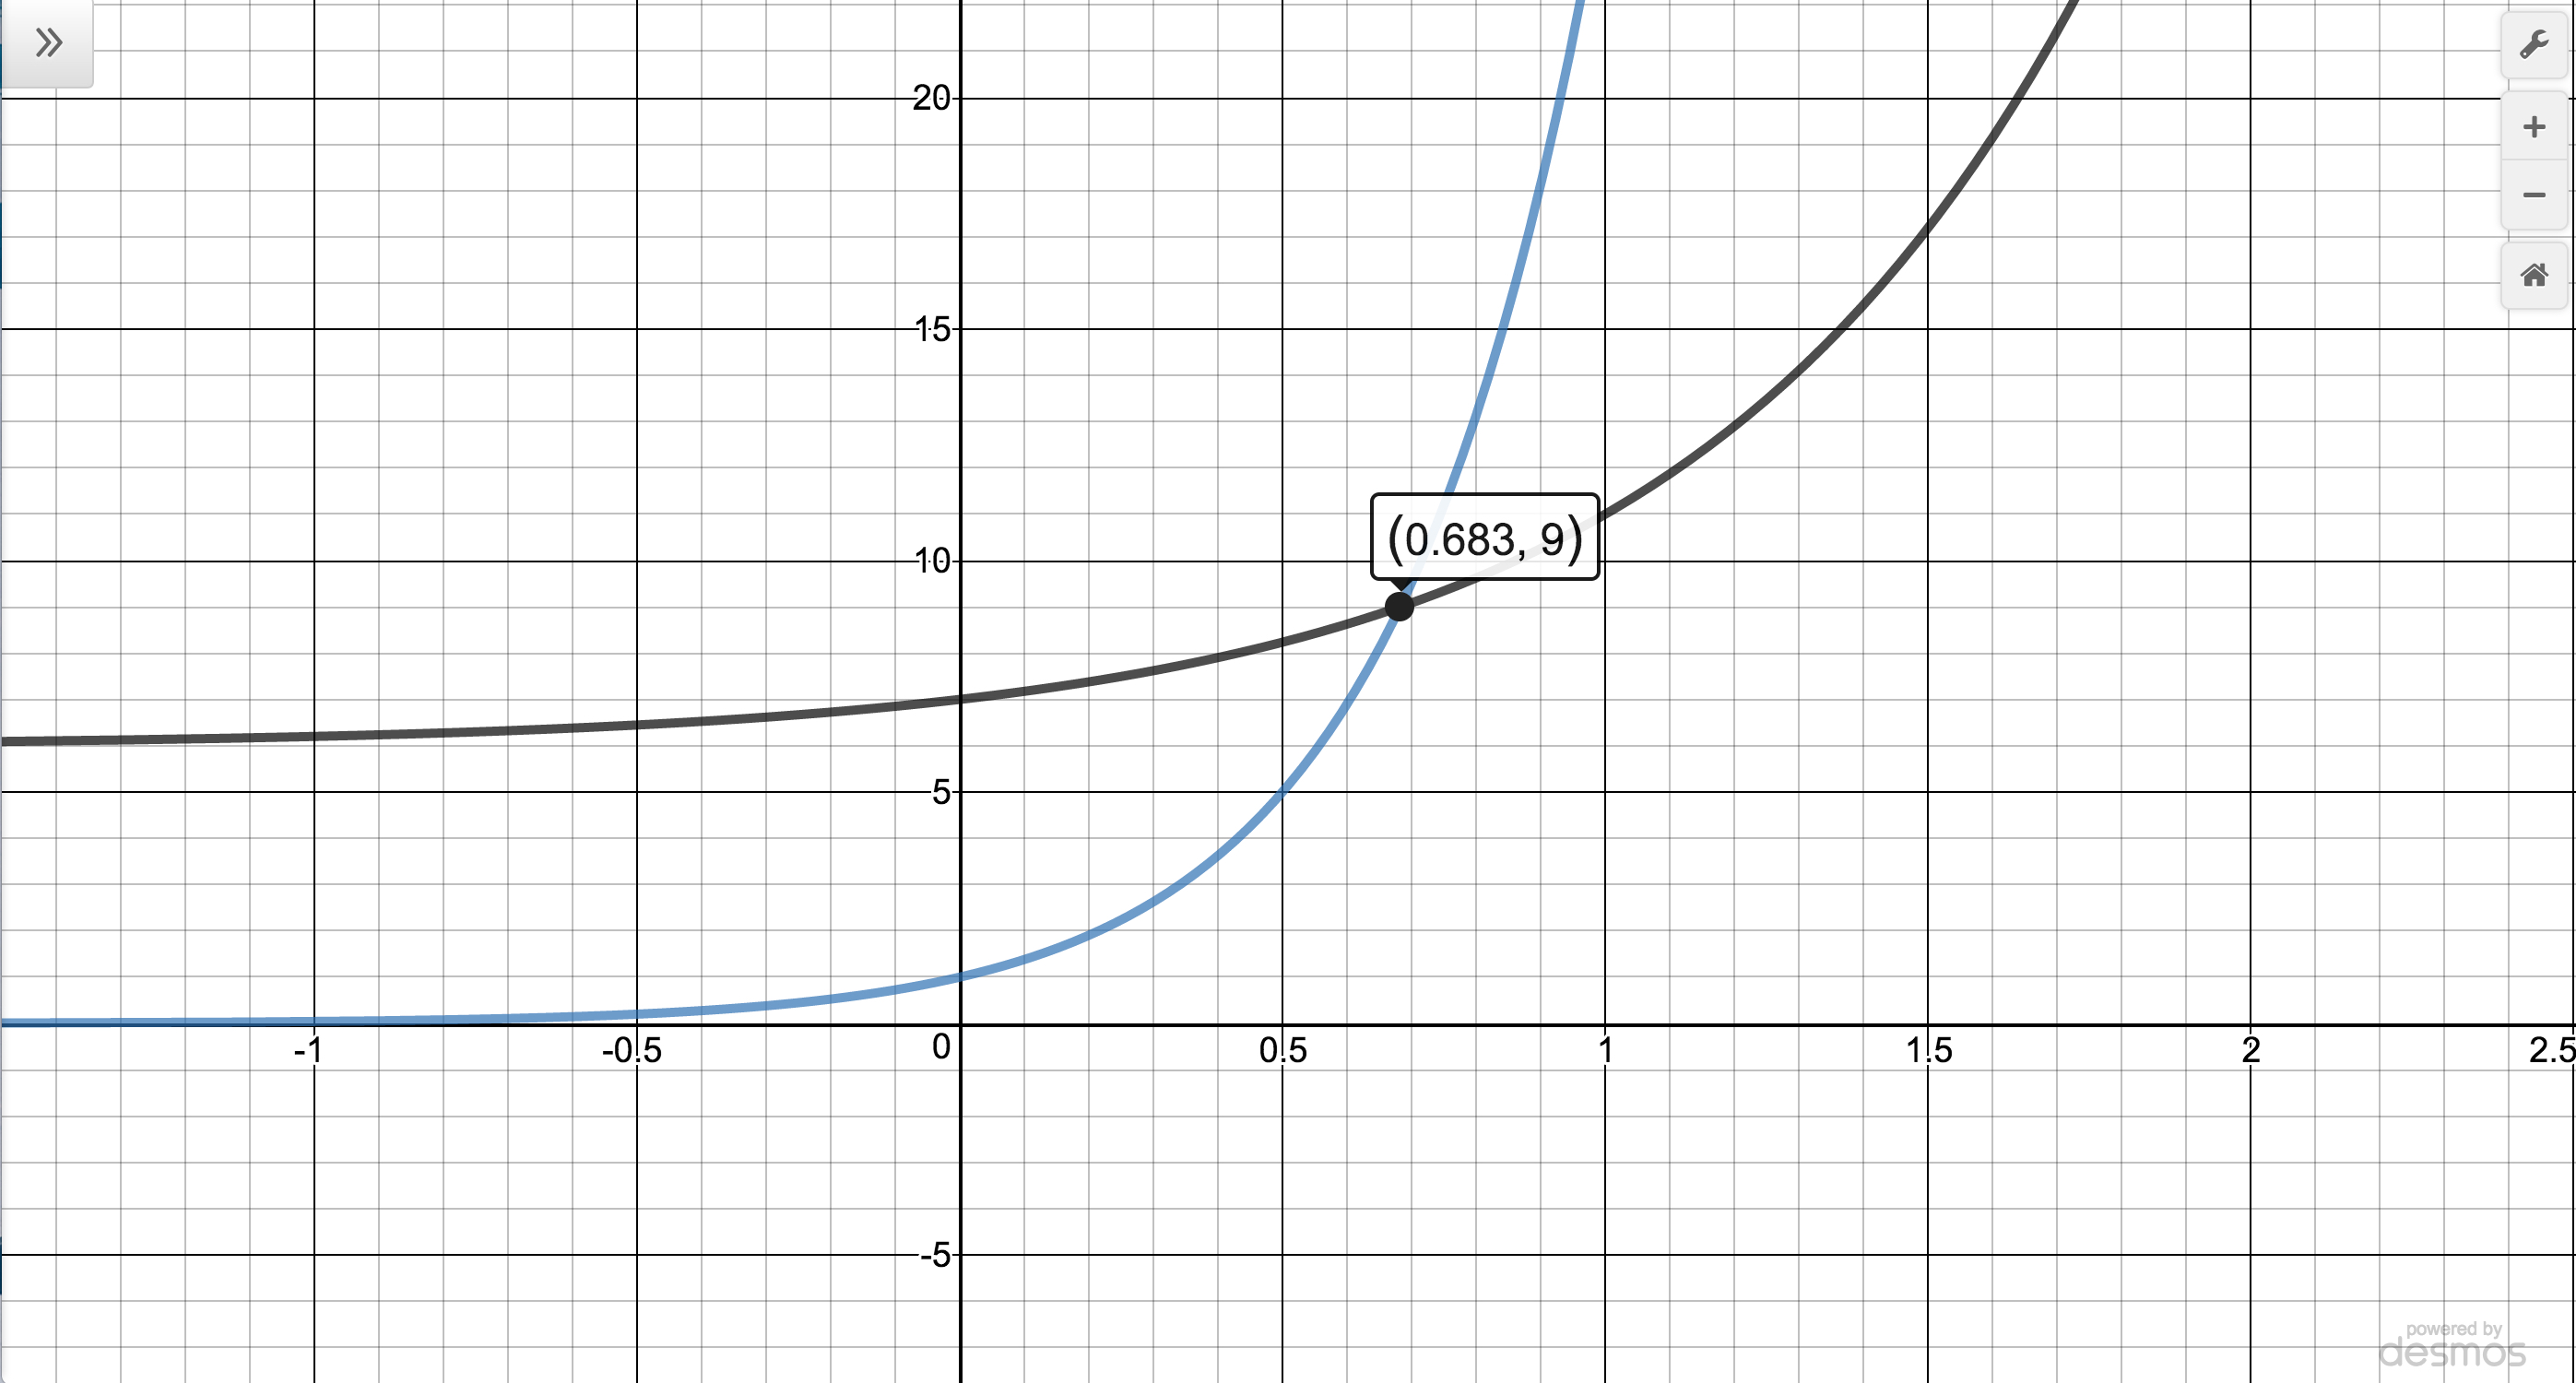
\includegraphics[width=3in]{./ExponentialEquationsandInequalitiesGraphics/ExpEqnEx05.jpg} &

 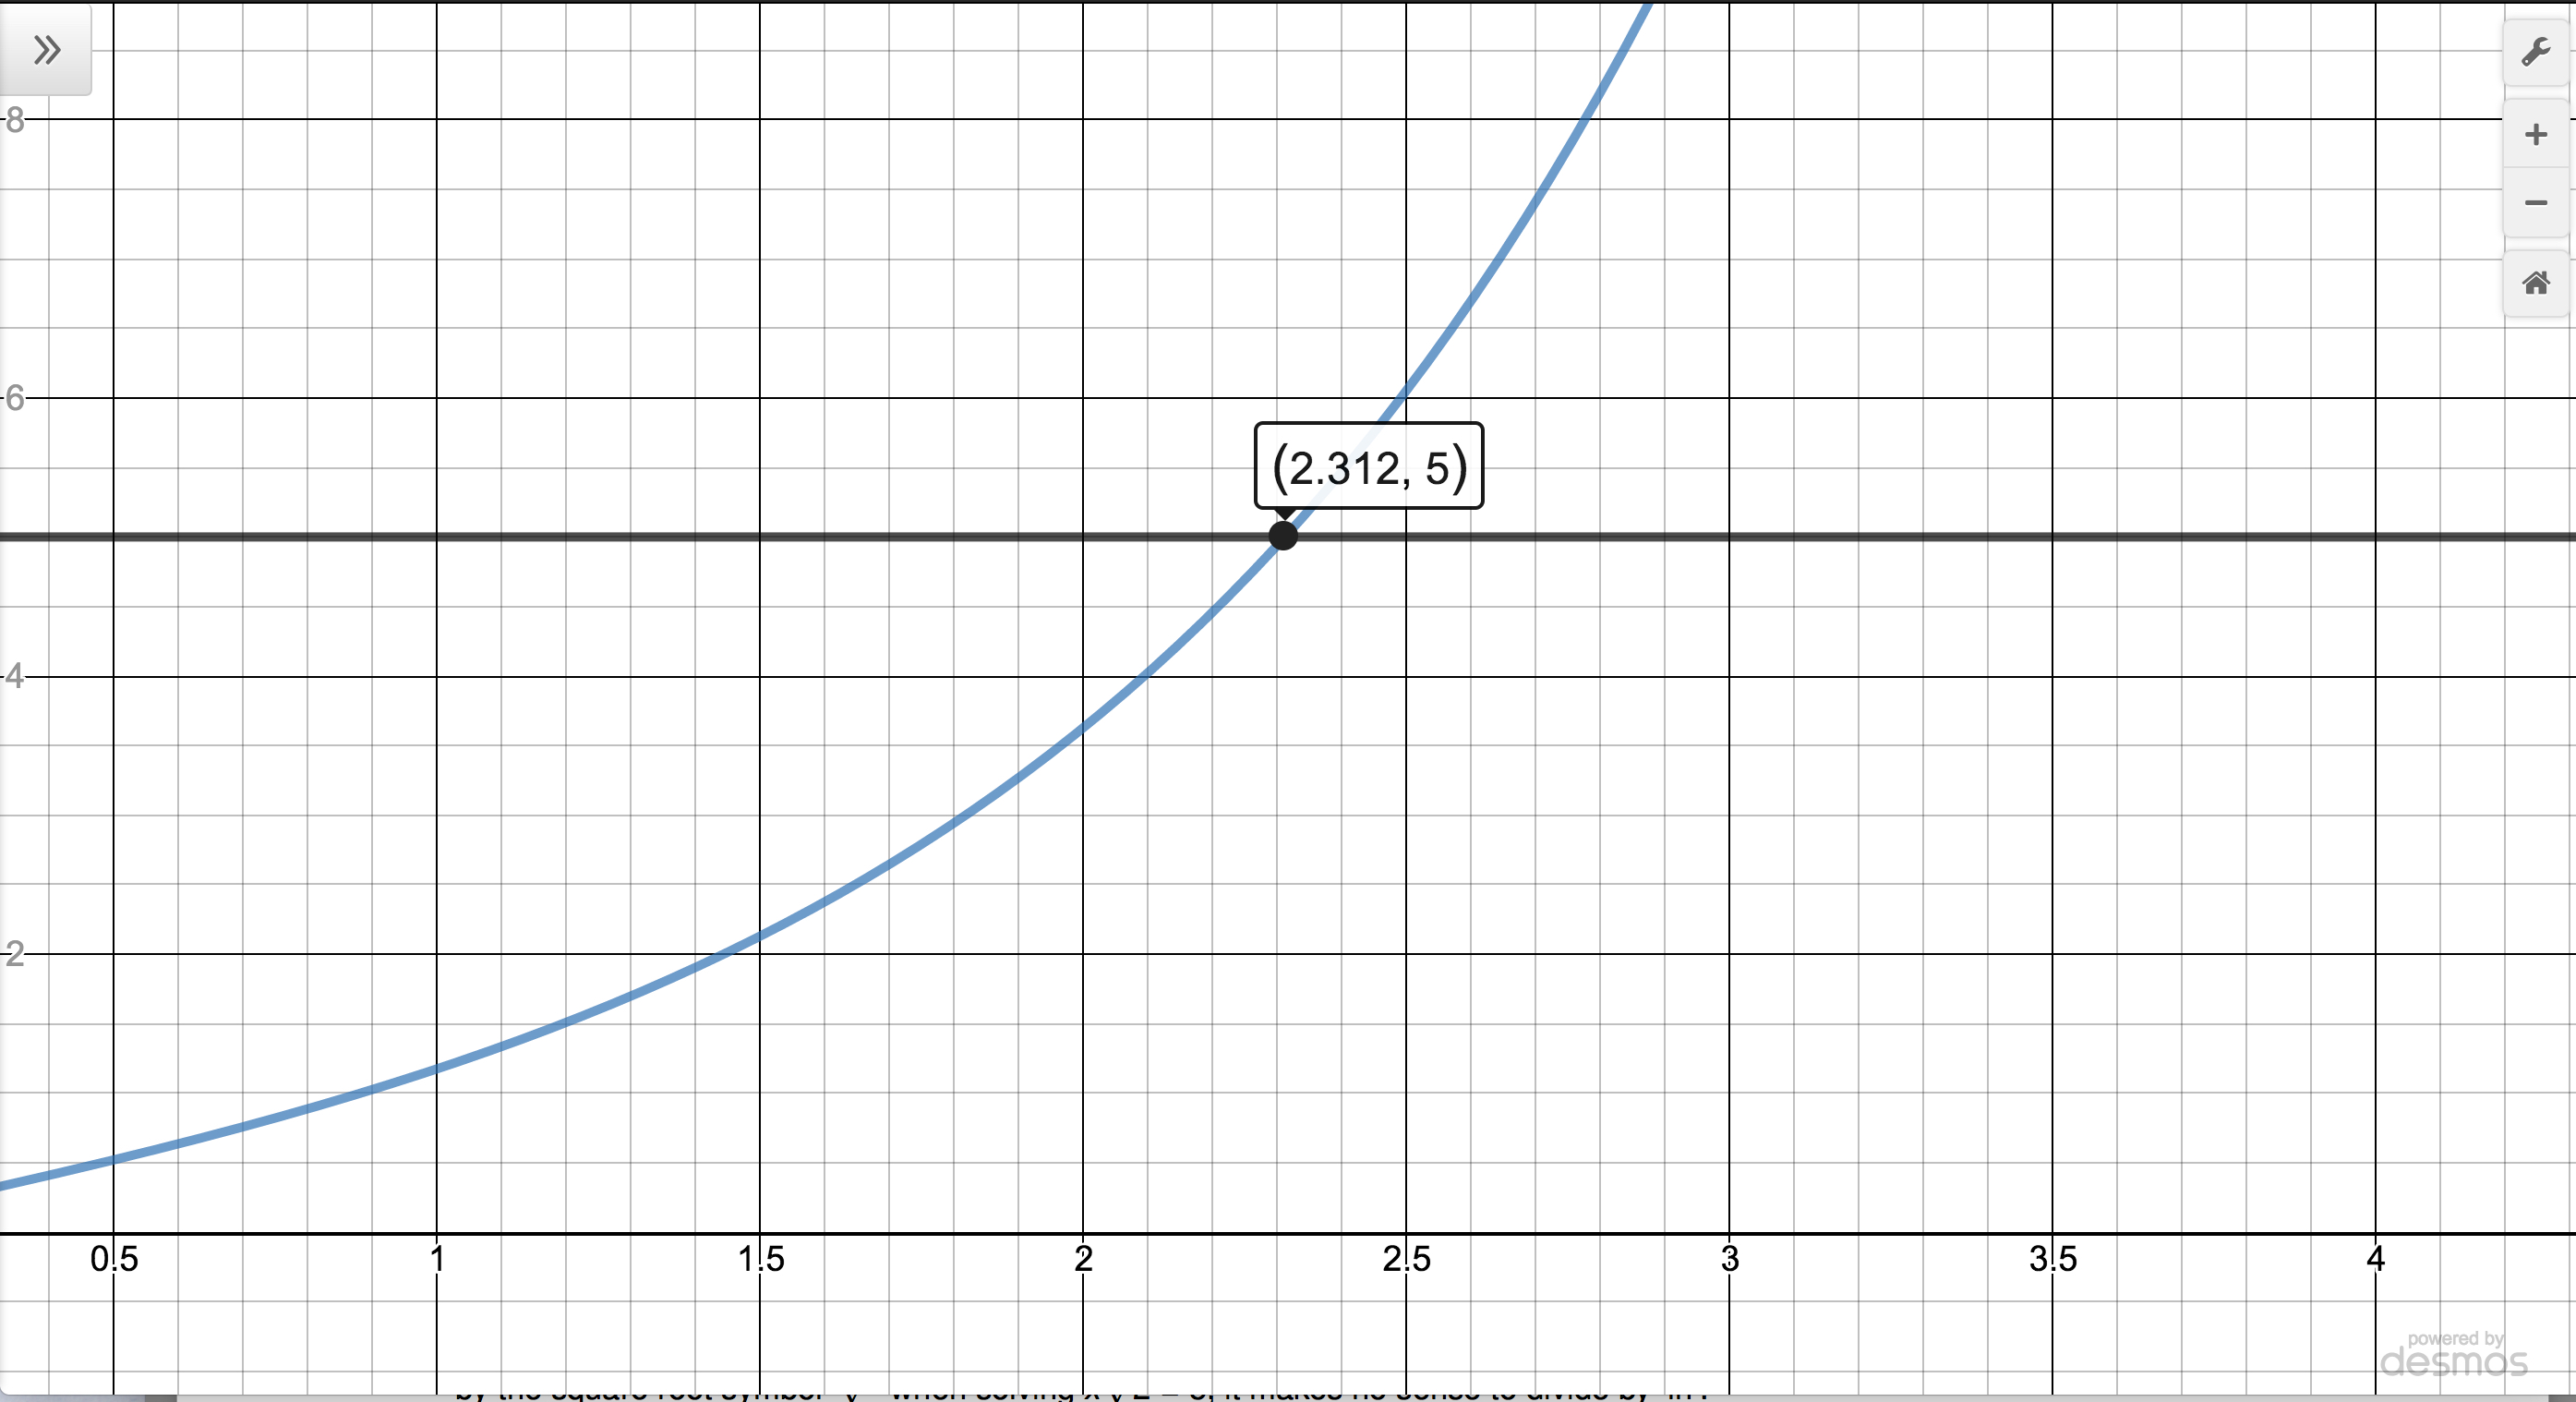
\includegraphics[width=3in]{./ExponentialEquationsandInequalitiesGraphics/ExpEqnEx06.jpg} \\

 Checking $25^{x} = 5^{x} + 6$
 
 &
 
 Checking   $\frac{e^{x} - e^{-x}}{2} = 5$
 
\end{tabular}

\end{center}


\end{enumerate}

\qed

\end{ex}

Note that verifying our solutions to the equations in Example \ref{expeqnsex1} \textit{analytically} holds great educational value, since it reviews many of the properties of logarithms and exponents in tandem.

\smallskip

For example, to verify our solution to  $2000 = 1000 \cdot 3^{-0.1 t}$, we substitute $t = -\frac{10\ln(2)}{\ln(3)}$ and check: 
\[ \begin{array}{rclr}

2000 & \stackrel{?}{=} & 1000 \cdot 3^{-0.1 \left(-\frac{10\ln(2)}{\ln(3)}\right)} & \\
2000 & \stackrel{?}{=} & 1000 \cdot 3^{\frac{\ln(2)}{\ln(3)}} & \\
2000 & \stackrel{?}{=} & 1000 \cdot 3^{\log_{3}(2)} & \mbox{Change of Base}\\
2000 & \stackrel{?}{=} & 1000 \cdot 2 & \mbox{Inverse Property}\\
2000 & \stackrel{\checkmark}{=} & 2000 & \\

\end{array}\]

We strongly encourage the reader to check the remaining equations analytically as well.

\smallskip

\begin{comment}
Since exponential functions are continuous on their domains, the Intermediate Value Theorem \ref{IVT} applies. This allows us to solve inequalities using sign diagrams as demonstrated below.

\begin{ex}  Solve the following inequalities.  Check your answer graphically.
\label{expineq}

\begin{multicols}{3}

\begin{enumerate}

\item \label{canuselogsex} $2^{x^2-3x} - 16 \geq 0$

\item  $\dfrac{e^{x}}{e^{x}-4} \leq 3$

\item  $t e^{2t} < 4t$

\end{enumerate}

\end{multicols}

\newpage

{\bf Solution.}

\begin{enumerate}

\item  Since we already have $0$ on one side of the inequality, we set $r(x) = 2^{x^2-3x} - 16$.  

\smallskip

The domain of $r$ is all real numbers, so to construct our sign diagram, we need to find the zeros of $r$.  

\smallskip

Setting $r(x) = 0$ gives $2^{x^2-3x} - 16 = 0$ or $2^{x^2-3x} = 16$.  Since $16 = 2^{4}$ we have $2^{x^2-3x} = 2^{4}$.   By the one-to-one property of exponential functions, $x^2 -3x = 4$ which gives $x=4$ and $x=-1$.  

\smallskip

From the sign diagram, we see $r(x) \geq 0$ on $(-\infty, -1] \cup [4, \infty)$, which is our solution.  

\smallskip

Graphing $r(x) = 2^{x^2-3x} - 16$,  we find it is on or above the line $y=0$ (the $x$-axis) precisely on the intervals  $(-\infty, -1]$ and $ [4, \infty)$ which checks our answer.

\begin{center}

\begin{tabular}{cc}

\begin{mfpic}[10]{-5}{5}{-1}{2}
\arrow \reverse \arrow \polyline{(-5,0),(5,0)}
\xmarks{-2,2}
\tlabel[cc](-3.5,1){$(+)$}
\tlabel[cc](-2,-1){$-1$}
\tlabel[cc](-2,1){$0$}
\tlabel[cc](0,1){$(-)$}
\tlabel[cc](2,-1){$4$}
\tlabel[cc](2,1){$0$}
\tlabel[cc](3.5,1){$(+)$}
\end{mfpic}

& 

 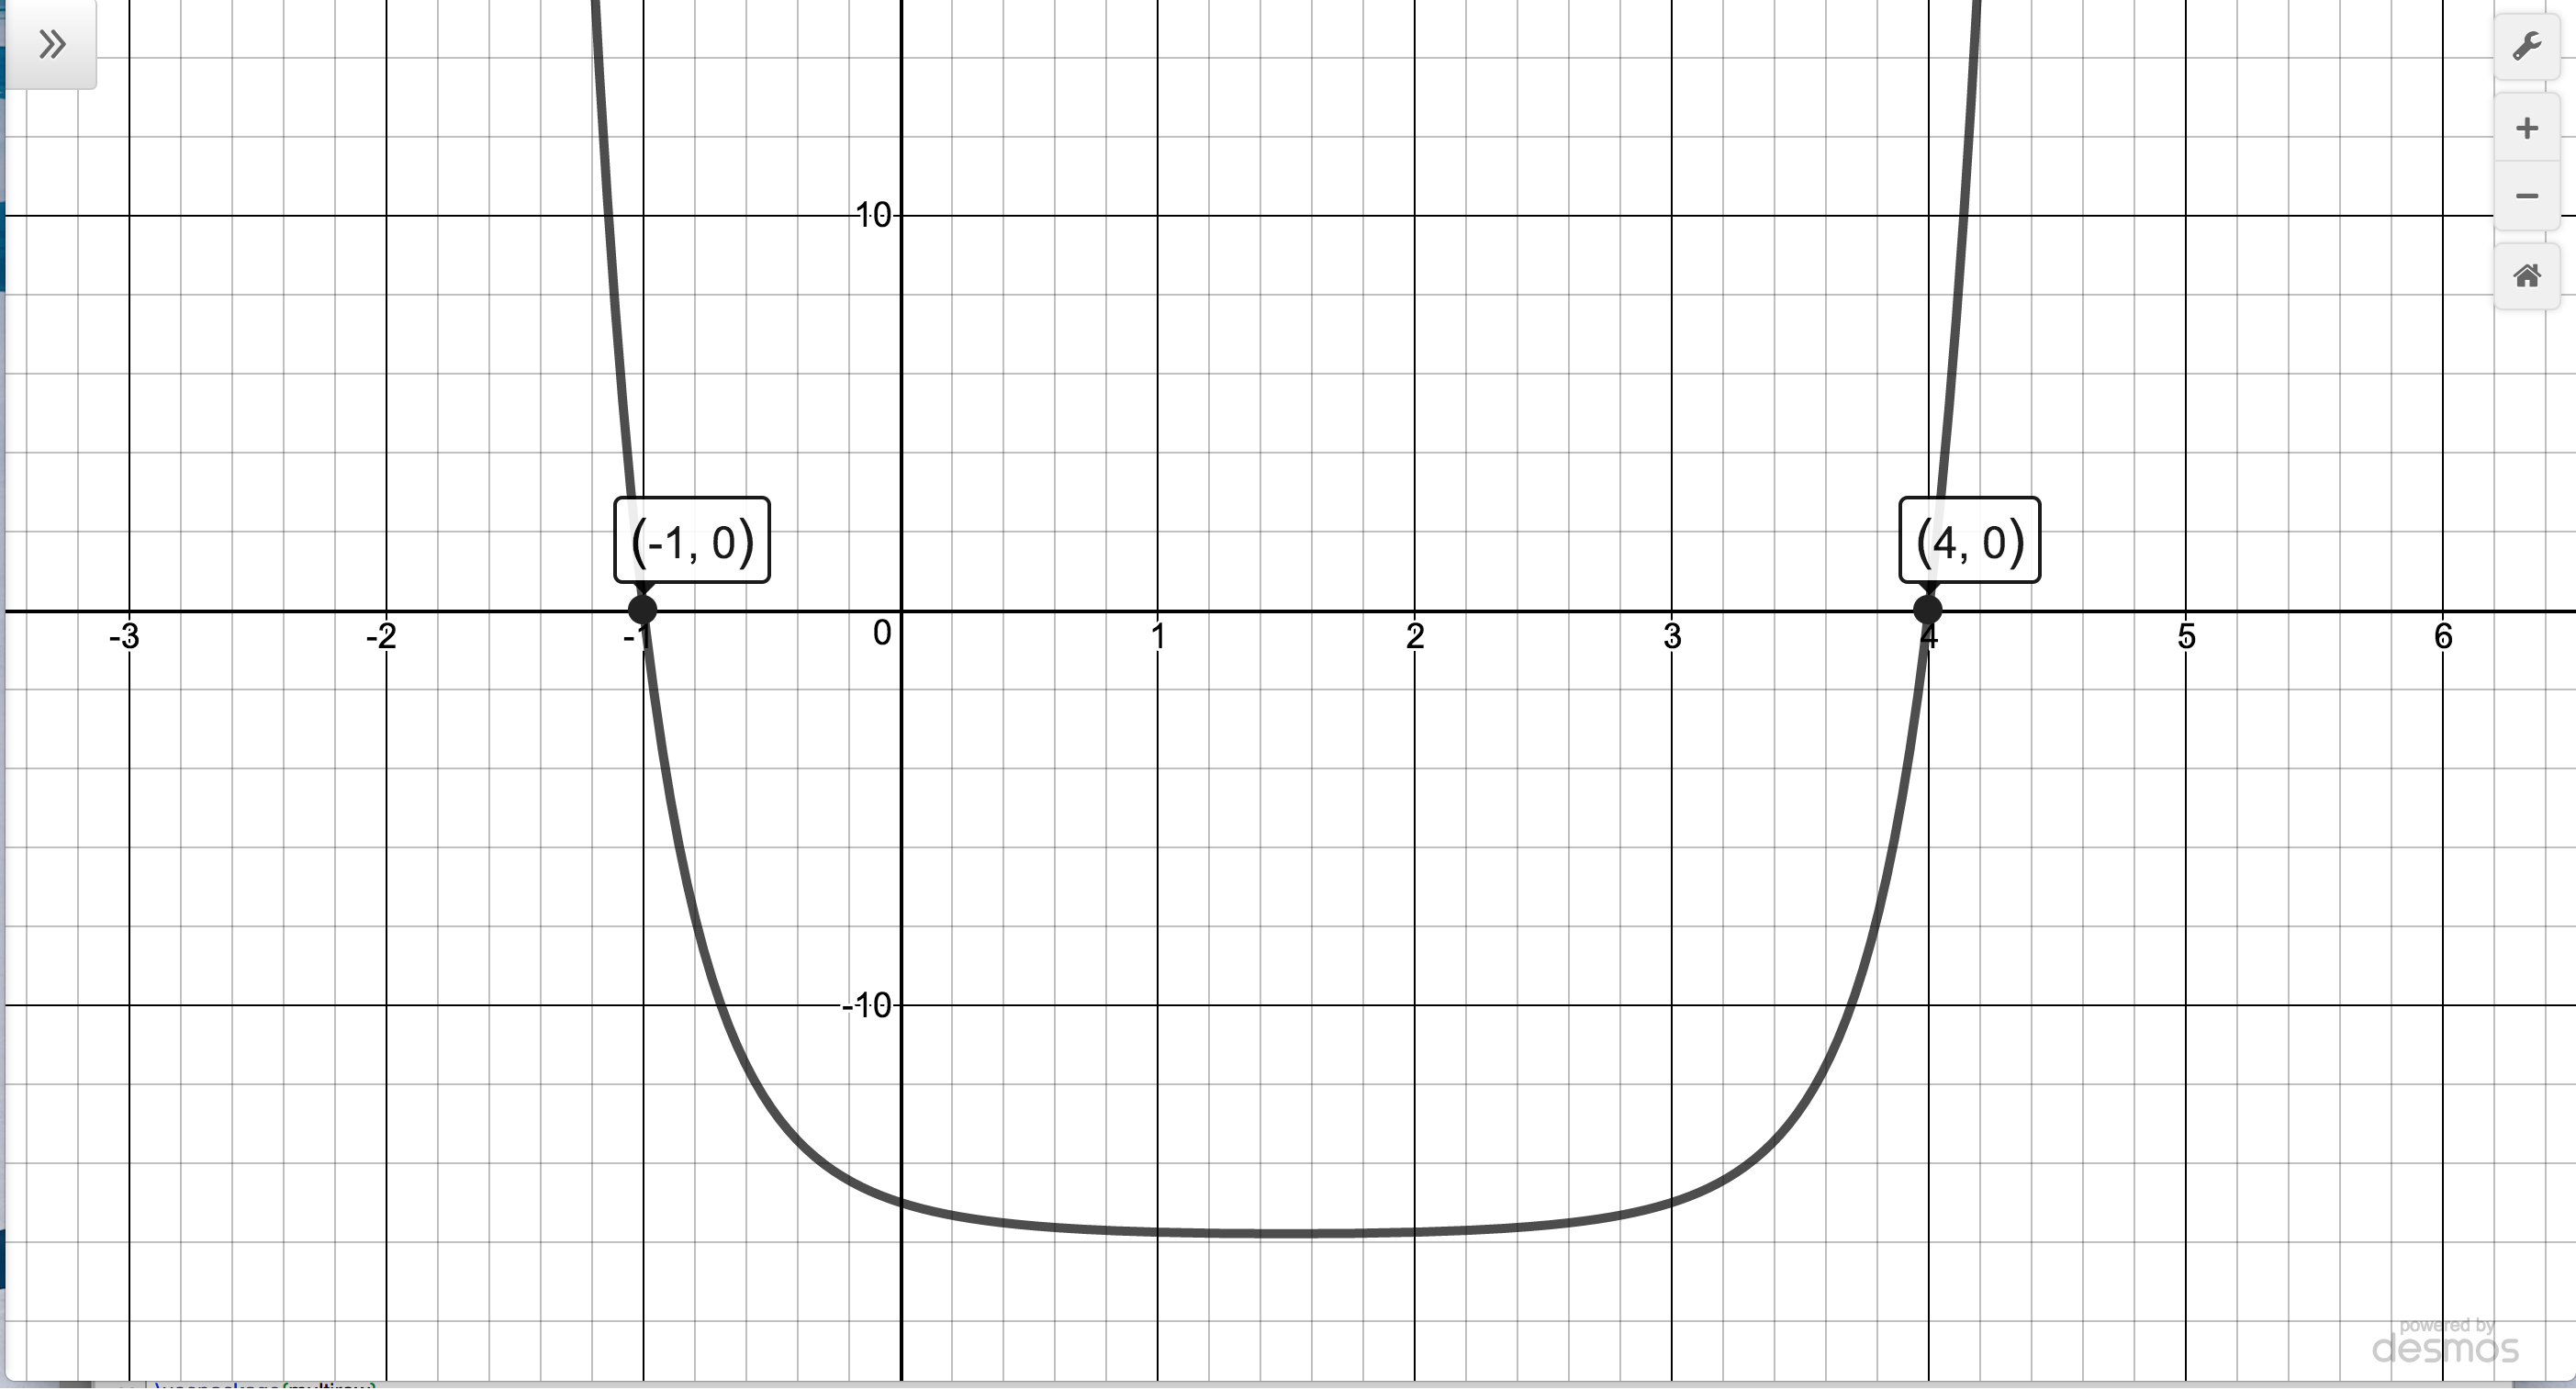
\includegraphics[width=3in]{./ExponentialEquationsandInequalitiesGraphics/ExpEqnEx07.jpg}  \\
 
 
A Sign Diagram for  $r(x) = 2^{x^2-3x} - 16$ & 

Checking $2^{x^2-3x} - 16 \geq 0$ \\

\end{tabular}

\end{center}

\item The first step we need to take to solve  $\frac{e^{x}}{e^{x}-4} \leq 3$ is to get $0$ on one side of the inequality. To that end, we subtract $3$ from both sides and get a common denominator


\setlength{\extrarowheight}{12pt}
\[ \begin{array}{rclr}

\dfrac{e^{x}}{e^{x}-4} & \leq & 3 & \\

\dfrac{e^{x}}{e^{x}-4} - 3 & \leq & 0 & \\

\dfrac{e^{x}}{e^{x}-4} - \dfrac{3 \left(e^{x}-4\right)}{e^{x}-4} & \leq & 0 & \mbox{Common denomintors.} \\

\dfrac{12 - 2e^{x}}{e^{x}-4} & \leq & 0 & \\

\end{array}\]
\setlength{\extrarowheight}{2pt}

We set $r(x) = \frac{12 - 2e^{x}}{e^{x}-4}$ and we note that $r$ is undefined when its denominator $e^{x}-4=0$, or when $e^{x} = 4$.  Solving this gives $x = \ln(4)$, so the domain of $r$ is $(-\infty, \ln(4)) \cup (\ln(4), \infty)$. 

\smallskip

To find the zeros of $r$, we solve $r(x) = 0$ and obtain $12 - 2e^{x} = 0$.  We find $e^{x} = 6$, or $x = \ln(6)$.  

\smallskip

When we build our sign diagram, finding test values may be a little tricky since we need to check values around $\ln(4)$ and $\ln(6)$.  

\smallskip

Recall that the function $\ln(x)$ is increasing\footnote{This is because the base of $\ln(x)$ is $e > 1$.  If the base $b$ were in the interval $0 < b < 1$, then $\log_{b}(x)$ would decreasing.} which means $\ln(3) < \ln(4) < \ln(5) < \ln(6) < \ln(7)$.  

\smallskip

To determine the sign of $r\left(\ln(3)\right)$, we remember that $e^{\ln(3)} = 3$ and get \[r\left(\ln(3)\right) = \frac{12 - 2e^{\ln(3)}}{e^{\ln(3)}-4} = \frac{12-2(3)}{3-4} = -6.\]  

We determine the signs of $r\left(\ln(5)\right)$ and $r\left(\ln(7)\right)$ similarly.\footnote{We could, of course, use the calculator, but what fun would that be?} From the sign diagram, we find our answer to be $(-\infty,\ln(4)) \cup [\ln(6), \infty)$.  


\smallskip

Using a graphing utility, we find the graph of $f(x) = \frac{e^{x}}{e^{x}-4}$ is below the graph of $g(x) = 3$ on $(-\infty,\ln(4)) \cup (\ln(6), \infty)$, and they intersect at $x  \approx 1.792 \approx  \ln(6)$.


\begin{center}

\begin{tabular}{cc}

\begin{mfpic}[10]{-5}{5}{-1}{2}
\arrow \reverse \arrow \polyline{(-5,0),(5,0)}
\xmarks{-2,2}
\tlabel[cc](-3.5,1){$(-)$}
\tlabel[cc](-2,-1){$\ln(4)$}
\tlabel[cc](-2,1){\textinterrobang}
\tlabel[cc](0,1){$(+)$}
\tlabel[cc](2,-1){$\ln(6)$}
\tlabel[cc](2,1){$0$}
\tlabel[cc](3.5,1){$(-)$}
\end{mfpic}

& 

 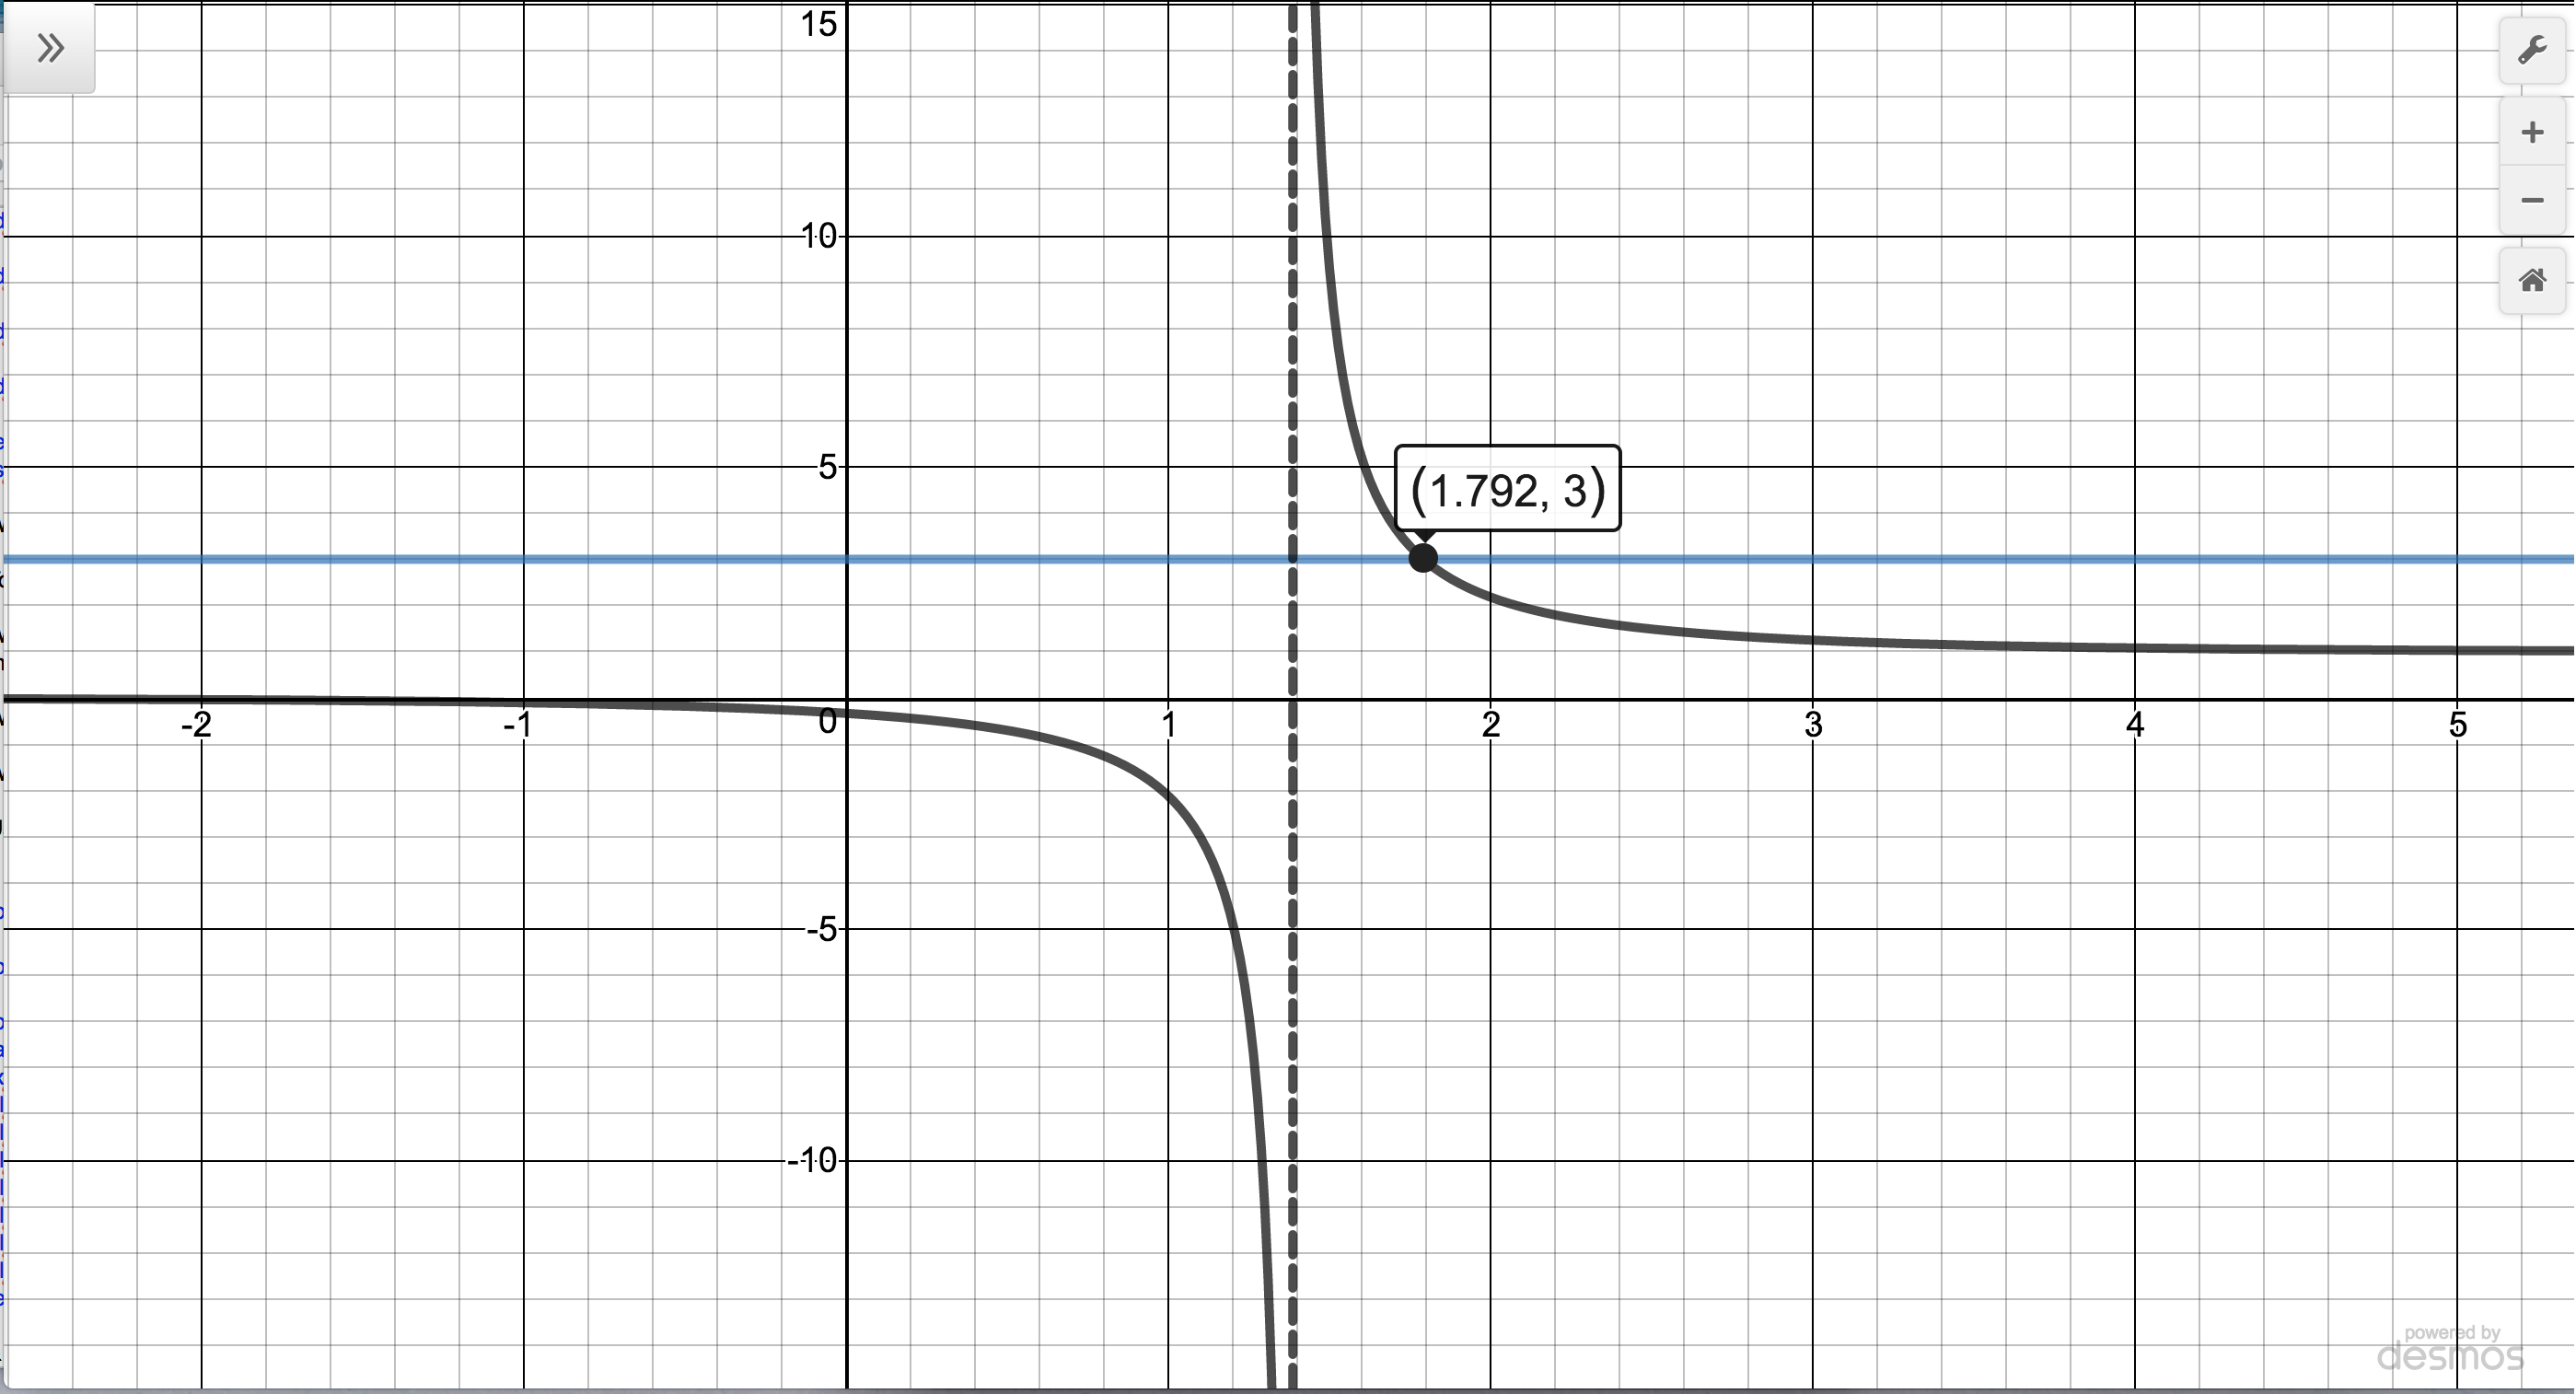
\includegraphics[width=3in]{./ExponentialEquationsandInequalitiesGraphics/ExpEqnEx08.jpg}  \\
 
 A Sign Diagram for  $r(x) = \dfrac{12 - 2e^{x}}{e^{x}-4}$ & 

Checking $\dfrac{e^{x}}{e^{x}-4} \leq 3$ \\

\end{tabular}

\end{center}


\item  As before, we start solving $t e^{2t} < 4t$ by getting $0$ on one side of the inequality, $t e^{2t} - 4t < 0$.   

\smallskip

We set $r(t) = te^{2t} - 4t$ and since there are no denominators, even-indexed radicals, or logs, the domain of $r$ is all real numbers.  

\smallskip

Setting $r(t) = 0$  produces $t e^{2t} - 4t  = 0$. We factor to get $t \left(e^{2t} - 4\right)  = 0$ which gives $t=0$ or $e^{2t} - 4 = 0$.  

\smallskip

To solve the latter, we isolate the exponential and take logs to get $2t = \ln(4)$, or $t = \frac{\ln(4)}{2}$ which simplifies to $t = \ln(2)$.  (Can you see why?)  

\smallskip

As in the previous example, we need to be careful about choosing test values.  Since $\ln(1) = 0$, we choose $\ln\left(\frac{1}{2}\right)$, $\ln\left(\frac{3}{2}\right)$ and $\ln(3)$.  Evaluating,\footnote{A calculator can be used at this point. As usual, we proceed without apologies, with the analytical method.} we get 

\[\begin{array}{rclr}

r\left(\ln\left(\frac{1}{2}\right)\right) & = & \ln\left(\frac{1}{2}\right) e^{2\ln\left(\frac{1}{2}\right)} - 4\ln\left(\frac{1}{2}\right) & \\

&= & \ln\left(\frac{1}{2}\right)e^{\ln\left(\frac{1}{2}\right)^2}- 4\ln\left(\frac{1}{2}\right) & \text{Power Rule} \\

& = & \ln\left(\frac{1}{2}\right)e^{\ln\left(\frac{1}{4}\right)}- 4\ln\left(\frac{1}{2}\right) & \\

& = & \frac{1}{4}  \ln\left(\frac{1}{2}\right) - 4  \ln\left(\frac{1}{2}\right) =  -\frac{15}{4} \ln\left(\frac{1}{2}\right) & \end{array}\] 

Since $\frac{1}{2} < 1$, $ \ln\left(\frac{1}{2}\right) < 0$ and we get $r(\ln\left(\frac{1}{2}\right))$ is $(+)$.  Proceeding similarly, we find $r\left(\ln\left(\frac{3}{2}\right)\right)  < 0$ and $r(\ln(3)) > 0$.  Our solution corresponds to $r(t) < 0$ which occurs on $(0 ,\ln(2))$.  

\smallskip

The graphing utility confirms that the graph of $f(t) = t e^{2t} $ is below the graph of $g(t) = 4t$ on $(0 ,\ln(2))$.\footnote{Note: $\ln(2) \approx 0.693$.}


\begin{center}

\begin{tabular}{cc}

\begin{mfpic}[10]{-5}{5}{-1}{2}
\arrow \reverse \arrow \polyline{(-5,0),(5,0)}
\xmarks{-2,2}
\tlabel[cc](-3.5,1){$(+)$}
\tlabel[cc](-2,-1){$0$}
\tlabel[cc](-2,1){0}
\tlabel[cc](0,1){$(-)$}
\tlabel[cc](2,-1){$\ln(2)$}
\tlabel[cc](2,1){$0$}
\tlabel[cc](3.5,1){$(+)$}
\end{mfpic}

& 

 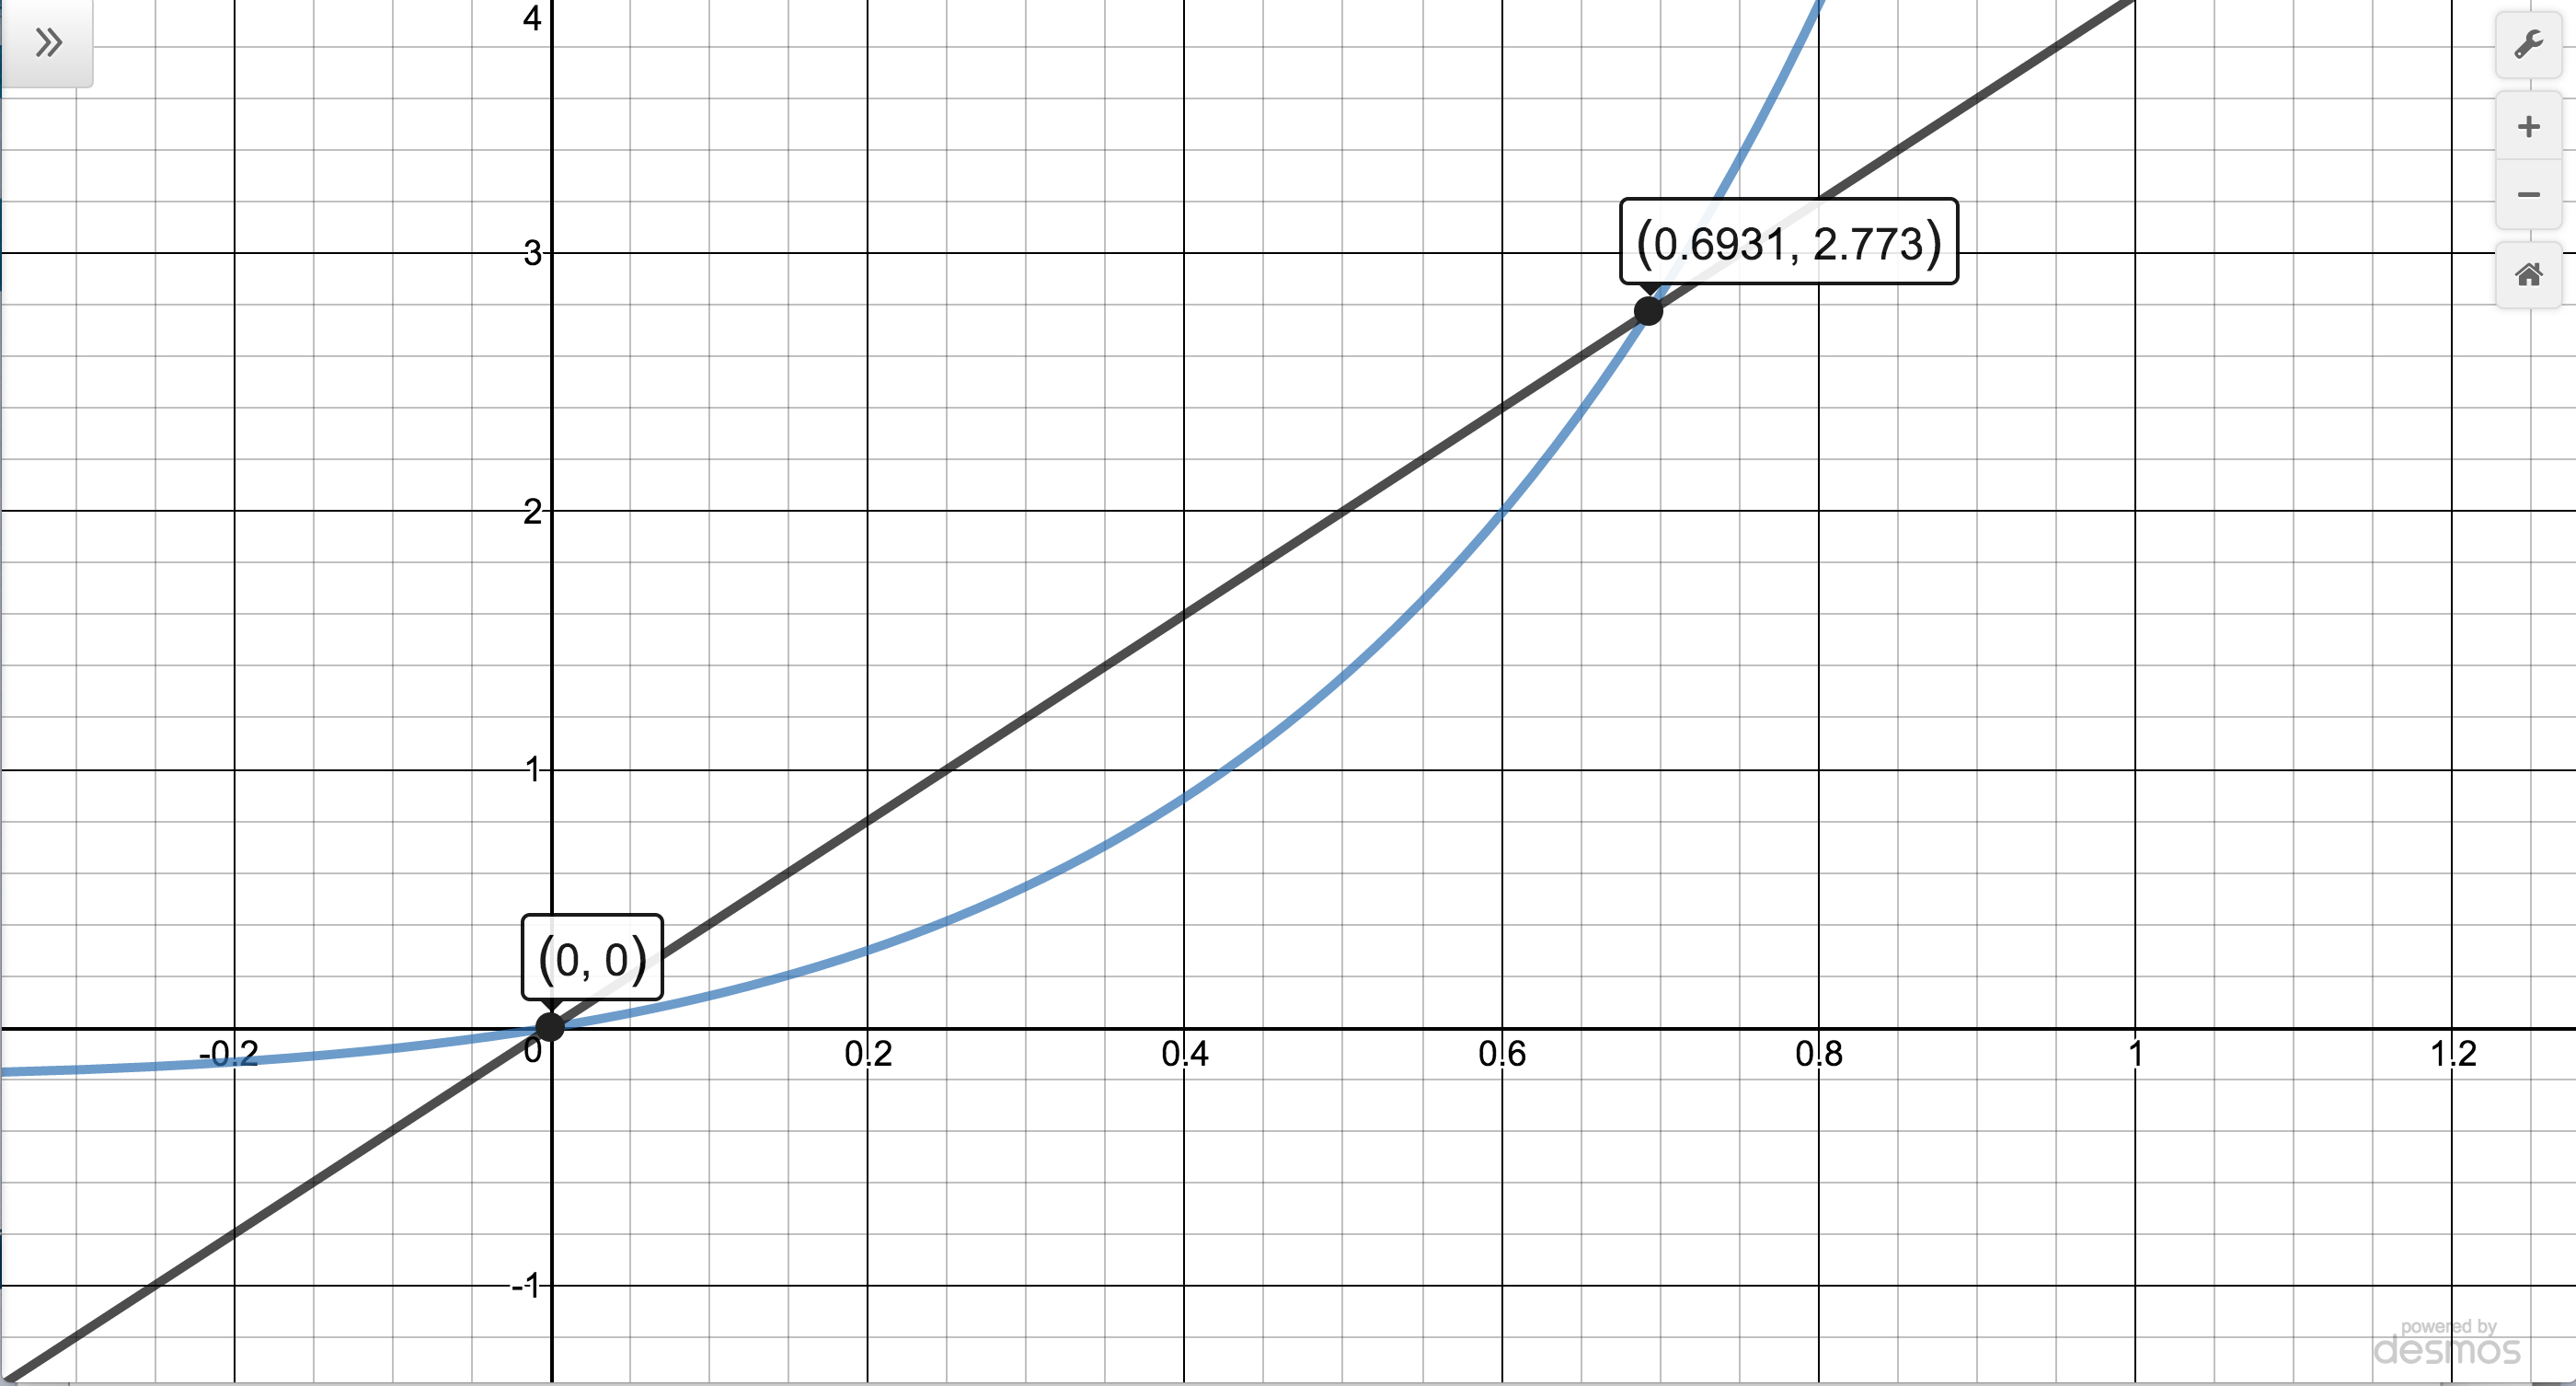
\includegraphics[width=3in]{./ExponentialEquationsandInequalitiesGraphics/ExpEqnEx09.jpg}  \\
 
 A Sign Diagram for  $r(t) = te^{2t} - 4t$  & 

Checking $t e^{2t} < 4t$ \\

\end{tabular}

\end{center}

\end{enumerate}

\qed

\end{ex}

We note here that while sign diagrams will \textit{always} work for solving inequalities involving exponential functions, as we've seen previously, there are circumstances in which we can short-cut this method. 

\smallskip

For example, consider number \ref{canuselogsex} from Example \ref{expineq} above:  $2^{x^2-3x} - 16 \geq 0$.  Since the base $2>1$, $\log_{2}(x)$ is an \textit{increasing} function meaning it preserves inequalities.

\smallskip

We can use this to our advantage in this case and eliminate the exponential from the inequality altogether:

\[ \begin{array}{rclr}

2^{x^2-3x} - 16 &  \geq &  0 &  \\

2^{x^2-3x}  & \geq & 16 & \\

\log_{2}\left(2^{x^2-3x} \right) & \geq & \log_{2}(16) & \text{$f(x) = \log_{2}(x)$ is increasing so if $b \geq a$, $\log_{2}(b) \geq \log_{2}(a)$. } \\

x^2 - 3x & \geq & 4 &\\ \end{array} \]

Hence, we've  reduced our given inequality to $x^2-3x \geq 4$.  As seen in Section \ref{QuadraticFunctions}, we can solve this inequality by completing the square, graphing, or a sign diagram, whichever strikes the reader's fancy.

\smallskip

Our next example is a follow-up to Example \ref{exptempex} in Section \ref{ExponentialFunctions}.  

\smallskip

\begin{ex}  \label{coffeewarmerex} Recall from Example \ref{exptempex}  the temperature of coffee $T$ (in degrees Fahrenheit) $t$ minutes after it is served can be modeled by $T(t) = 70 + 90 e^{-0.1 t}$.  When will the coffee be warmer than $100^{\circ}\mbox{F}$?

\smallskip

{\bf Solution.}  We need to find when $T(t) > 100$, that is, we need to solve  $70 + 90 e^{-0.1 t} > 100$.  

\smallskip

To use a sign diagram, we need to get $0$ on one side of the inequality.  Subtracting $100$ from both sides of $70 + 90 e^{-0.1 t} > 100$ produces   $90 e^{-0.1 t} - 30 > 0$. 

\smallskip

Identifying  $r(t) = 90 e^{-0.1 t} - 30$, we note from the context of the problem the domain of $r$ is $[0, \infty)$, so to build the sign diagram, we proceed to find the zeros of $r$.  

\smallskip

Solving $90 e^{-0.1 t} - 30=0$ results in $e^{-0.1t} = \frac{1}{3}$ so that $t = -10\ln\left(\frac{1}{3}\right)$  which reduces to $t = 10 \ln(3)$.

\smallskip

If we wish to avoid using the calculator to choose test values, we note that $f(x)  = \ln(x)$ is increasing.  As a result,  since $1 < 3$, $0 = \ln(1) < \ln(3)$ which proves $10\ln(3) > 0$. Hence, we may choose $t = 0$ as a test value in $[0, 10 \ln(3))$.  Since $3 < 4$, $\ln(3) < \ln(4)$, so $10 \ln(3) < 10 \ln(4)$. Hence,  we may choose $10 \ln(4)$   as test value for the interval $(10 \ln(3), \infty)$. 

\smallskip

We find $r(0)>0$ and $r(10\ln(4))<0$  which gives  the sign diagram below. We see $r(t)>0$ on $[0, 10\ln(3))$.

\smallskip

We graph $y=T(t)$ from Example  \ref{exptempex} below on the right along with with the horizontal line $y = 100$.   We see the graph of $T$ is above the horizontal line to the left of the intersection point, which we leave to the reader to show is $(10 \ln(3), 100)$.

\begin{center}

\begin{tabular}{m{0.5in}m{2.5in}m{2.5in}}

&

\begin{mfpic}[10]{0}{8}{-2}{2}
\arrow \polyline{(0,0), (8,0)}
\xmarks{0,4}
\tlabel[cc](0,-1){$0$}
\tlabel[cc](0,1){$(+)$}
\tlabel[cc](4,-1){ $10 \ln(3)$}
\tlabel[cc](4,1){$0$}
\tlabel[cc](6,1){$(-)$}
\end{mfpic}

& 

\begin{mfpic}[15]{-1}{11}{-1}{10}
\point[2pt]{(0,8)}
\dashed \polyline{(-1,3.5),(11,3.5)}
\axes
\tlabel[cc](9,3){\scriptsize H.A. $y=70$}
\tlabel[cc](9,5.5){\scriptsize $y=100$}
\tlabel[cc](11,-0.5){\scriptsize $t$}
\tlabel[cc](0.5,10){\scriptsize $y$}
\tcaption{\scriptsize $y = T(t)$}
\ymarks{1,2,3,4,5,6,7,8,9}
\xmarks{1,2,3,4,5,6,7,8,9,10}
\tlpointsep{4pt}
\axislabels {x}{{\scriptsize $2$} 1, {\scriptsize $4$} 2, {\scriptsize $6$} 3, {\scriptsize $8$} 4,{\scriptsize $10$} 5, {\scriptsize $12$} 6, {\scriptsize $14$} 7, {\scriptsize $16$} 8, {\scriptsize $18$} 9, {\scriptsize $20$} 10}
\axislabels {y}{{\scriptsize $20$} 1, {\scriptsize $40$} 2, {\scriptsize $60$} 3,{\scriptsize $80$} 4, {\scriptsize $120$} 6,{\scriptsize $140$} 7, {\scriptsize $160$} 8, {\scriptsize $180$} 9}
\penwd{1.25pt}
\arrow \reverse \arrow \polyline{(-1,5),(11,5)}
\arrow \function{0, 10, 0.1}{(90*exp(0-0.2*x)+70)/20}
\point[4pt]{(0,8), (5.5,5)}
\end{mfpic} \\

\end{tabular}

\end{center}

Hence, the coffee is warmer than $100^{\circ}$F up to $10 \ln(3) \approx 11$ minutes after it is served, or, said differently, it takes approximately 11 minutes for the coffee to cool to under $100^{\circ}$F.  \qed

\end{ex}

We note that, once again, we can short-cut the sign diagram in Example \ref{coffeewarmerex} to solve $70 + 90 e^{-0.1 t} > 100$.  Since $\ln(x)$ is increasing, it preserves inequality.  This means we can solve this inequality as follows.

\[ \begin{array}{rclr}

70 + 90 e^{-0.1 t} & > & 100 & \\
90 e^{-0.1 t} & > & 30 & \\
e^{-0.1 t} > & \frac{1}{3} & \\
\ln \left( e^{-0.1 t} \right) & > & \ln \left( \frac{1}{3} \right) & \text{$f(x) = \ln(x)$ is increasing so if $b \geq a$, $\ln(b) \geq  \ln(a)$. } \\
-0.1 t & > & - \ln(3) & \text{$\ln \left( \frac{1}{3} \right) = \ln \left(3^{-1} \right) = - \ln(3)$.} \\
t & < & \frac{-\ln(3)}{-0.1} = 10 \ln(3) & \\ \end{array} \]

Since we are given $t \geq 0$, we arrive at the same answer $0 \leq t < 10\ln(3)$ or $[0, 10 \ln(3))$.  

\smallskip

Note the importance, once again, of having a base larger than $1$ so that the corresponding logarithmic function is \textit{increasing}.  We can still adapt this strategy to exponential functions whose base is less than $1$, but we need to remember the corresponding logarithmic function is \textit{decreasing} so it \textit{reverses}  inequalities.  

 \smallskip

We close this section by finding a function inverse.

\newpage

\begin{ex}  \label{expfracinverse} The function $f(x) = \dfrac{5e^{x}}{e^{x}+1}$ is one-to-one. 

\begin{multicols}{2} 

\begin{enumerate}

\item Find a formula for $f^{-1}(x)$.

\item  Solve $\dfrac{5e^{x}}{e^{x}+1} = 4$.

\end{enumerate}

\end{multicols}

{\bf Solution.}  \begin{enumerate} \item We start by writing $y=f(x)$, and interchange the roles of $x$ and $y$.  To solve for $y$, we first clear denominators and then isolate the exponential function.

\[ \begin{array}{rclr}
y & = & \dfrac{5e^{x}}{e^{x}+1} & \\ [12pt]
x & = & \dfrac{5e^{y}}{e^{y}+1} & \mbox{Switch $x$ and $y$} \\ [12pt]
x \left(e^{y}+1\right) & = & 5e^{y} & \\ [4pt]
x e^{y}+x & = & 5e^{y} & \\ [4pt]
x & = & 5e^{y} - x e^{y} & \\ [4pt]
x & = & e^{y}(5 - x) & \\ [4pt]
e^{y}& = & \dfrac{x}{5-x} & \\[12pt]
\ln\left(e^{y}\right) & = & \ln\left(\dfrac{x}{5-x}\right) & \\[12pt]
y & = & \ln\left(\dfrac{x}{5-x}\right) & \\
\end{array}\]

We claim $f^{-1}(x) = \ln\left(\frac{x}{5-x}\right)$.  To verify this analytically, we would need to verify the compositions $\left(f^{-1} \circ f\right)(x) = x$ for all $x$ in the domain of $f$ and that $\left(f \circ f^{-1}\right)(x) = x$ for all $x$ in the domain of $f^{-1}$.   We leave this, as well as a graphical check, to the reader in Exercise \ref{checkingexpfracinverse}.

%To verify our solution graphically, we graph $y = f(x) = \frac{5e^{x}}{e^{x}+1}$ and $y = g(x) = \ln\left(\frac{x}{5-x}\right)$ on the same set of axes and observe the symmetry about the line $y=x$ below.
%\begin{center}

% 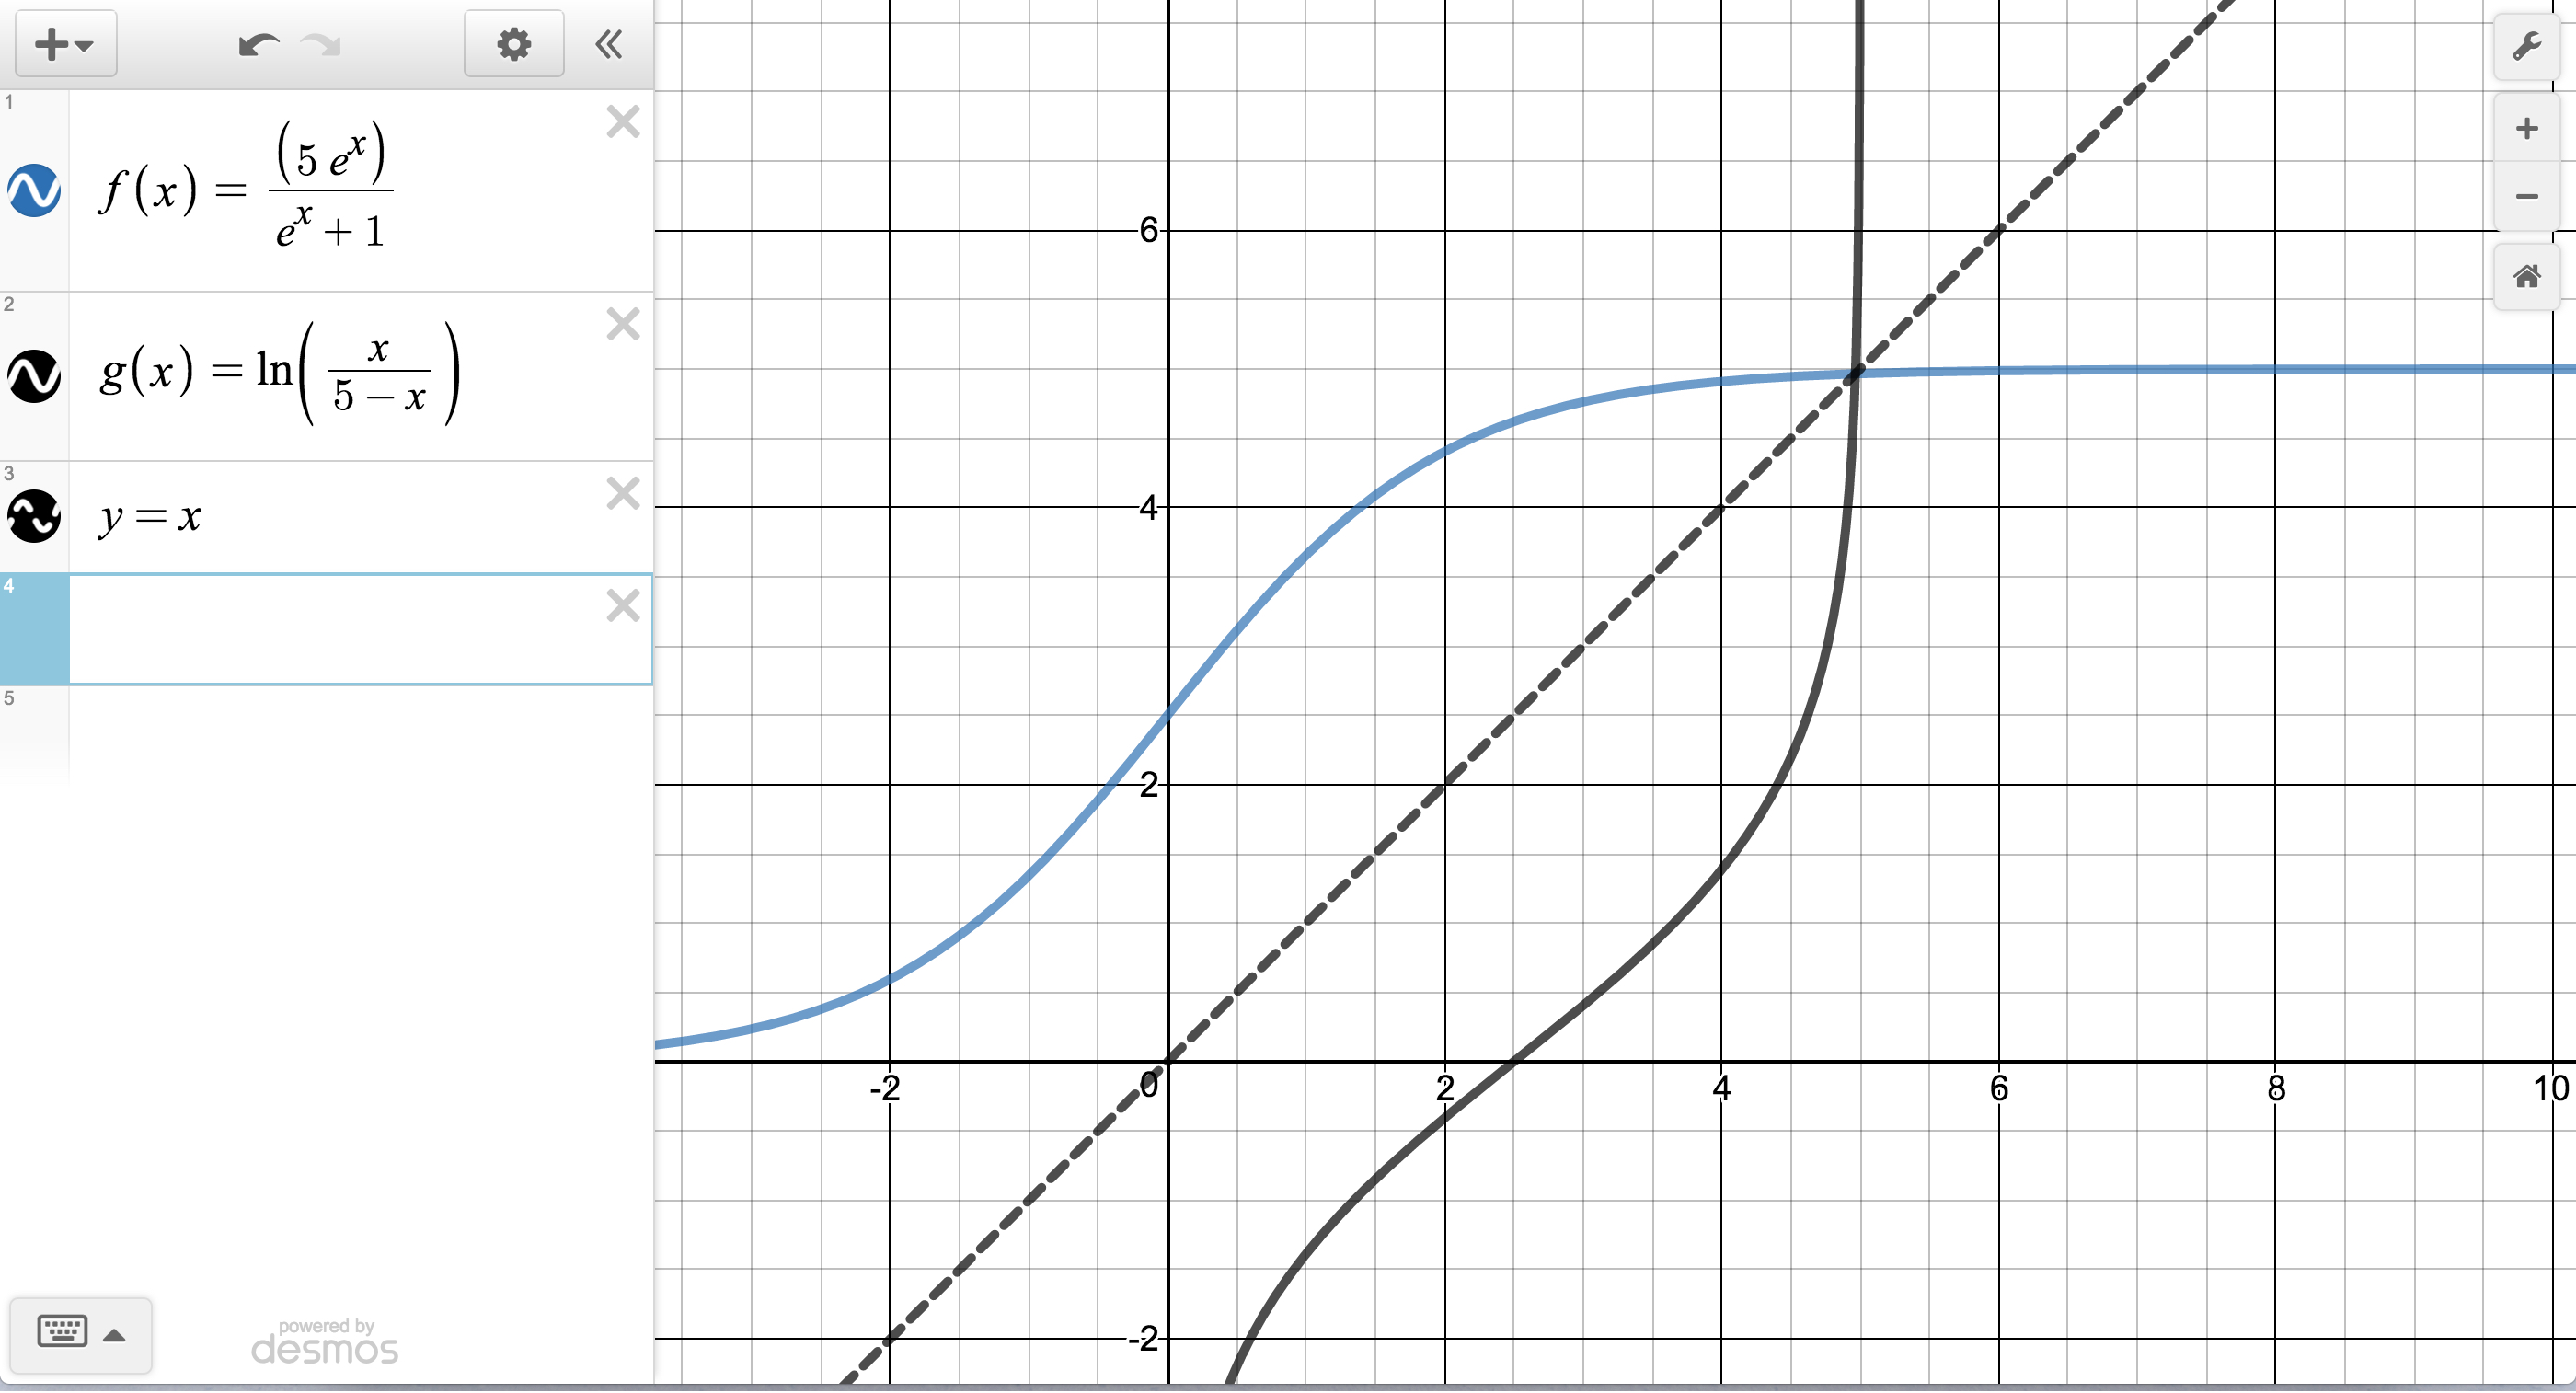
\includegraphics[width=4in]{./ExponentialEquationsandInequalitiesGraphics/ExpEqnEx10.jpg}

%\end{center}

\item We recognize the equation $\frac{5e^{x}}{e^{x}+1} = 4$ as $f(x) = 4$.  Hence, our solution is $x = f^{-1}(4) = \ln\left(\frac{4}{5-4}\right) = \ln(4)$.  

We can check this fairly quickly algebraically.  Using  $e^{\ln(4)} = 4$, we find $\frac{5e^{\ln(4)}}{e^{\ln(4)}+1}  = \frac{5(4)}{4+1} = \frac{20}{5} = 4$. \qed

\end{enumerate}

\end{ex}

\end{comment}


\newpage

\subsection{Exercises}

\label{ExercisesforExponentialEquationsandInequalities}

In Exercises \ref{expeqnfirst} - \ref{expeqnlast}, solve the equation analytically.

\begin{multicols}{3}
\begin{enumerate}

\item $2^{4x} = 8$  \label{expeqnfirst} 
\item $3^{(x - 1)} = 27$  
\item $5^{2x-1} = 125$ 

\setcounter{HW}{\value{enumi}}
\end{enumerate}
\end{multicols}

\begin{multicols}{3}
\begin{enumerate}
\setcounter{enumi}{\value{HW}}

\item $4^{2t} = \frac{1}{2}$
\item $8^{t} = \frac{1}{128}$ 
\item $2^{(t^{3} - t)} = 1$ \vphantom{ $8^{t} = \frac{1}{128}$}

\setcounter{HW}{\value{enumi}}
\end{enumerate}
\end{multicols}

\begin{multicols}{3}
\begin{enumerate}
\setcounter{enumi}{\value{HW}}

\item $3^{7x} = 81^{4-2x}$ 
\item $9 \cdot 3^{7x} = \left(\frac{1}{9}\right)^{2x}$ 
\item $3^{2x} = 5$ 

\setcounter{HW}{\value{enumi}}
\end{enumerate}
\end{multicols}

\begin{multicols}{3}
\begin{enumerate}
\setcounter{enumi}{\value{HW}}

\item $5^{-t} = 2$ 
\item $5^{t} = -2$  
\item $3^{(t - 1)} = 29$  

\setcounter{HW}{\value{enumi}}
\end{enumerate}
\end{multicols}

\begin{multicols}{3}
\begin{enumerate}
\setcounter{enumi}{\value{HW}}

\item $(1.005)^{12x} = 3$
\item $e^{-5730k} = \frac{1}{2}$ 
\item $2000e^{0.1t} = 4000$  

\setcounter{HW}{\value{enumi}}
\end{enumerate}
\end{multicols}

\begin{multicols}{3}
\begin{enumerate}
\setcounter{enumi}{\value{HW}}


\item $500\left(1-e^{2t}\right) = 250$
\item $70 + 90e^{-0.1t} = 75$ 
\item $30-6e^{-0.1t}=20$ 


\setcounter{HW}{\value{enumi}}
\end{enumerate}
\end{multicols}

\begin{multicols}{3}
\begin{enumerate}
\setcounter{enumi}{\value{HW}}

\item $\dfrac{100e^{x}}{e^{x}+2}=50$ 
\item $\dfrac{5000}{1+2e^{-3t}}=2500$ 
\item $\dfrac{150}{1 + 29e^{-0.8t}} = 75$ 


\setcounter{HW}{\value{enumi}}
\end{enumerate}
\end{multicols}

\begin{multicols}{3}
\begin{enumerate}
\setcounter{enumi}{\value{HW}}

\item $25\left(\frac{4}{5}\right)^{x} = 10$  

\item $e^{2x} = 2e^{x}$ 
\item  $7e^{2t} = 28e^{-6t}$ 

\setcounter{HW}{\value{enumi}}
\end{enumerate}
\end{multicols}

\begin{multicols}{3}
\begin{enumerate}
\setcounter{enumi}{\value{HW}}

\item $3^{(x - 1)} = 2^{x}$ 
\item $3^{(x - 1)} = \left(\frac{1}{2}\right)^{(x + 5)}$ 
\item  $7^{3+7x} = 3^{4-2x}$  

\setcounter{HW}{\value{enumi}}
\end{enumerate}
\end{multicols}

\begin{multicols}{3}
\begin{enumerate}
\setcounter{enumi}{\value{HW}}

\item $e^{2t} - 3e^{t}-10=0$ %Ans $t=\ln(5)$
\item $e^{2t} = e^{t}+6$ %Ans $t=\ln(2)$
\item $4^{t} + 2^{t} = 12$ %Ans $x=\dfrac{\ln(3)}{\ln(2)}$


\setcounter{HW}{\value{enumi}}
\end{enumerate}
\end{multicols}

\begin{multicols}{3}
\begin{enumerate}
\setcounter{enumi}{\value{HW}}

\item $e^{x}-3e^{-x}=2$ %Ans $x=\ln(3)$
\item $e^{x}+15e^{-x}=8$ %Ans $x=\ln(2)$, $\ln(5)$
\item $3^{x}+25\cdot3^{-x}=10$ %Ans $x=\dfrac{\ln(5)}{\ln(3)}$
\label{expeqnlast} 

\setcounter{HW}{\value{enumi}}
\end{enumerate}
\end{multicols}

In Exercises \ref{expineqfirst} - \ref{expineqlast}, solve the inequality analytically.

\begin{multicols}{2} 
\begin{enumerate}
\setcounter{enumi}{\value{HW}}

\item $e^{x} > 53$ \label{expineqfirst} 
\item $1000\left(1.005\right)^{12t} \geq 3000$ 

\setcounter{HW}{\value{enumi}}
\end{enumerate}
\end{multicols}

\begin{multicols}{2} 
\begin{enumerate}
\setcounter{enumi}{\value{HW}}

\item $2^{(x^{3} - x)} < 1$
\item $25\left(\dfrac{4}{5}\right)^{x} \geq 10$

\setcounter{HW}{\value{enumi}}
\end{enumerate}
\end{multicols}

\begin{multicols}{2} 
\begin{enumerate}
\setcounter{enumi}{\value{HW}}

\item $\dfrac{150}{1 + 29e^{-0.8t}} \leq 130$

\item $\vphantom{\dfrac{150}{1 + 29e^{-0.8t}}} 70 + 90e^{-0.1t} \leq 75$

\setcounter{HW}{\value{enumi}}
\end{enumerate}
\end{multicols}

\begin{multicols}{2} 
\begin{enumerate}
\setcounter{enumi}{\value{HW}}

\item $e^{-x} - xe^{-x} \geq 0$
\item $(1-e^{t}) t^{-1} \leq 0$ \label{expineqlast}

\setcounter{HW}{\value{enumi}}
\end{enumerate}
\end{multicols}

In Exercises \ref{calcexpineqfirst} - \ref{calcexpineqlast},  use a graphing utility to help you solve the equation or  inequality.

\begin{multicols}{3} 
\begin{enumerate}
\setcounter{enumi}{\value{HW}}

\item $2^{x} = x^2$ \label{calcexpineqfirst} 
\item $e^{t} = \ln(t) + 5$   
\item $e^{\sqrt{x}} = x + 1$ 

\setcounter{HW}{\value{enumi}}
\end{enumerate}
\end{multicols}

\begin{multicols}{3} 
\begin{enumerate}
\setcounter{enumi}{\value{HW}}

\item  $e^{-2t}-te^{-t} \geq 0$
\item $3^{(x - 1)} < 2^{x}$ 
\item $e^{t} < t^{3} - t$ \label{calcexpineqlast} 

\setcounter{HW}{\value{enumi}}
\end{enumerate}
\end{multicols}

\pagebreak

In Exercises \ref{domaincomplicatedexpfirst} - \ref{domaincomplicatedexplast},  find the domain of the function.

\begin{multicols}{2} 
\begin{enumerate}
\setcounter{enumi}{\value{HW}}

\item  $T(x) = \dfrac{e^{x} - e^{-x}}{e^{x} + e^{-x}}$     \label{domaincomplicatedexpfirst}

\item   $C(x) = \dfrac{e^{x}  + e^{-x}}{e^{x}  - e^{-x}}$ 

\setcounter{HW}{\value{enumi}}
\end{enumerate}
\end{multicols}


\begin{multicols}{2} 
\begin{enumerate}
\setcounter{enumi}{\value{HW}}

\item     $s(t) = \sqrt{e^{2t} - 3}$
\item     $c(t) = \sqrt[3]{e^{2t} - 3}$

\setcounter{HW}{\value{enumi}}
\end{enumerate}
\end{multicols}

\begin{multicols}{2} 
\begin{enumerate}
\setcounter{enumi}{\value{HW}}
  
\item     $L(x) = \log\left( 3 - e^{x} \right)$  \vphantom{$\ell(x) = \ln\left( \dfrac{e^{2x}}{e^{x}-2} \right)$}

\item    $\ell(x) = \ln\left( \dfrac{e^{2x}}{e^{x}-2} \right)$  \label{domaincomplicatedexplast}

\setcounter{HW}{\value{enumi}}
\end{enumerate}
\end{multicols}




\begin{enumerate}
\setcounter{enumi}{\value{HW}}

\item \label{onetoonelogexercise} Since $f(x) = \ln(x)$ is a strictly increasing function, if $0 < a < b$ then $\ln(a) < \ln(b)$.  Use this fact to solve the inequality $e^{(3x - 1)} > 6$ without a sign diagram. Use this technique to solve the inequalities in Exercises \ref{expineqfirst} - \ref{expineqlast}. (NOTE:  Isolate the exponential function first!)

\item \label{hyperbolicsine} Compute the inverse of $f(x) = \dfrac{e^{x} - e^{-x}}{2}$.  State the domain and range of both $f$ and $f^{-1}$. 

\item \label{checkingexpfracinverse} \co{In Example \ref{expfracinverse}, we found that t}The inverse of $f(x) = \dfrac{5e^{x}}{e^{x}+1}$ was $f^{-1}(x) = \ln\left(\dfrac{x}{5-x}\right)$\co{ but we left a few loose ends for you to tie up}.  

\begin{enumerate}

\item Algebraically check our answer by verifying: $\left(f^{-1} \circ f\right)(x) = x$ for all $x$ in the domain of $f$ and that $\left(f \circ f^{-1}\right)(x) = x$ for all $x$ in the domain of $f^{-1}$.

\item Find the range of $f$ by finding the domain of $f^{-1}$.

\item With help of a graphing utility, graph $y = f(x)$,  $y = f^{-1}(x)$ and $y = x$ on the same set of axes.  How does this help to verify our answer?

\item Let $g(x) = \dfrac{5x}{x+1}$ and $h(x) = e^{x}$.  Show that $f = g \circ h$ and that $(g \circ h)^{-1} = h^{-1} \circ g^{-1}$. 

NOTE:  We know this is true in general by Exercise \ref{fcircginverse} in Section \ref{InverseFunctions}, but it's nice to see a specific example of the property.

\end{enumerate}

\item With the help of your classmates, solve the inequality $e^{x} > x^{n}$ for a variety of natural numbers $n$.  What might you conjecture about the ``speed'' at which $f(x) = e^{x}$ grows versus any polynomial?

\end{enumerate}

\newpage

\subsection{Answers}


\begin{multicols}{3}
\begin{enumerate}

\item $x = \frac{3}{4}$
\item $x = 4$
\item $x=2$

\setcounter{HW}{\value{enumi}}
\end{enumerate}
\end{multicols}

\begin{multicols}{3}
\begin{enumerate}
\setcounter{enumi}{\value{HW}}

\item $t = -\frac{1}{4}$
\item $t = -\frac{7}{3}$
\item $t = -1, \, 0, \, 1$

\setcounter{HW}{\value{enumi}}
\end{enumerate}
\end{multicols}

\begin{multicols}{3}
\begin{enumerate}
\setcounter{enumi}{\value{HW}}

\item $x = \frac{16}{15}$
\item $x=-\frac{2}{11}$  \vphantom{$x = \dfrac{\ln(5)}{2\ln(3)}$}
\item $x = \dfrac{\ln(5)}{2\ln(3)}$

\setcounter{HW}{\value{enumi}}
\end{enumerate}
\end{multicols}

\begin{multicols}{3}
\begin{enumerate}
\setcounter{enumi}{\value{HW}}

\item $t = -\dfrac{\ln(2)}{\ln(5)}$
\item No solution. \vphantom{ $t = \dfrac{\ln(29) + \ln(3)}{\ln(3)}$}
\item $t = \dfrac{\ln(29) + \ln(3)}{\ln(3)}$

\setcounter{HW}{\value{enumi}}
\end{enumerate}
\end{multicols}

\begin{multicols}{3}
\begin{enumerate}
\setcounter{enumi}{\value{HW}}

\item $x = \dfrac{\ln(3)}{12\ln(1.005)}$ \vphantom{$k = \dfrac{\ln\left(\frac{1}{2}\right)}{-5730} = \dfrac{\ln(2)}{5730} $}
\item $k = \dfrac{\ln\left(\frac{1}{2}\right)}{-5730} = \dfrac{\ln(2)}{5730} $
\item $t=\dfrac{\ln(2)}{0.1} = 10\ln(2)$ \vphantom{$k = \dfrac{\ln\left(\frac{1}{2}\right)}{-5730} = \dfrac{\ln(2)}{5730} $}

\setcounter{HW}{\value{enumi}}
\end{enumerate}
\end{multicols}

\begin{multicols}{2}
\begin{enumerate}
\setcounter{enumi}{\value{HW}}


\item $t=\frac{1}{2}\ln\left(\frac{1}{2}\right) = -\frac{1}{2}\ln(2)$ \vphantom{$t = \dfrac{\ln\left(\frac{1}{18}\right)}{-0.1} =10 \ln(18)$}
\item $t = \dfrac{\ln\left(\frac{1}{18}\right)}{-0.1} =10 \ln(18)$

\setcounter{HW}{\value{enumi}}
\end{enumerate}
\end{multicols}

\begin{multicols}{2}
\begin{enumerate}
\setcounter{enumi}{\value{HW}}


\item $t=-10\ln\left(\frac{5}{3}\right) = 10\ln\left(\frac{3}{5}\right)$
\item$x=\ln(2)$ \vphantom{$t=-10\ln\left(\frac{5}{3}\right) = 10\ln\left(\frac{3}{5}\right)$}

\setcounter{HW}{\value{enumi}}
\end{enumerate}
\end{multicols}

\begin{multicols}{2}
\begin{enumerate}
\setcounter{enumi}{\value{HW}}

\item $t=\frac{1}{3}\ln(2)$ \vphantom{$t = \dfrac{\ln\left(\frac{1}{29}\right)}{-0.8} = \dfrac{5}{4}\ln(29)$}

\item $t = \dfrac{\ln\left(\frac{1}{29}\right)}{-0.8} = \dfrac{5}{4}\ln(29)$

\setcounter{HW}{\value{enumi}}
\end{enumerate}
\end{multicols}

\begin{multicols}{2}
\begin{enumerate}
\setcounter{enumi}{\value{HW}}

\item $x = \dfrac{\ln\left(\frac{2}{5}\right)}{\ln\left(\frac{4}{5}\right)} = \dfrac{\ln(2)-\ln(5)}{\ln(4) - \ln(5)}$

\item $x =  \ln(2)$ \vphantom{ $x = \dfrac{\ln\left(\frac{2}{5}\right)}{\ln\left(\frac{4}{5}\right)} = \dfrac{\ln(2)-\ln(5)}{\ln(4) - \ln(5)}$}


\setcounter{HW}{\value{enumi}}
\end{enumerate}
\end{multicols}

\begin{multicols}{2}
\begin{enumerate}
\setcounter{enumi}{\value{HW}}


\item  $t = -\frac{1}{8} \ln\left(\frac{1}{4} \right) = \frac{1}{4}\ln(2)$ \vphantom{$x = \dfrac{\ln(3)}{\ln(3) - \ln(2)}$}

\item $x = \dfrac{\ln(3)}{\ln(3) - \ln(2)}$

\setcounter{HW}{\value{enumi}}
\end{enumerate}
\end{multicols}

\begin{multicols}{2}
\begin{enumerate}
\setcounter{enumi}{\value{HW}}


\item $x = \dfrac{\ln(3) + 5\ln\left(\frac{1}{2}\right)}{\ln(3) - \ln\left(\frac{1}{2}\right)} = \dfrac{\ln(3)-5\ln(2)}{\ln(3)+\ln(2)}$
\item  $x = \dfrac{4 \ln(3) - 3 \ln(7)}{7 \ln(7) + 2 \ln(3)}$ \vphantom{$x = \dfrac{\ln(3) + 5\ln\left(\frac{1}{2}\right)}{\ln(3) - \ln\left(\frac{1}{2}\right)} = \dfrac{\ln(3)-5\ln(2)}{\ln(3)+\ln(2)}$}

\setcounter{HW}{\value{enumi}}
\end{enumerate}
\end{multicols}

\begin{multicols}{3}
\begin{enumerate}
\setcounter{enumi}{\value{HW}}

\item $t=\ln(5)$ \vphantom{$t=\dfrac{\ln(3)}{\ln(2)}$}
\item $t=\ln(3)$  \vphantom{$t=\dfrac{\ln(3)}{\ln(2)}$}
\item $t=\dfrac{\ln(3)}{\ln(2)}$


\setcounter{HW}{\value{enumi}}
\end{enumerate}
\end{multicols}

\begin{multicols}{3}
\begin{enumerate}
\setcounter{enumi}{\value{HW}}

\item $x=\ln(3)$  \vphantom{$x=\dfrac{\ln(5)}{\ln(3)}$}
\item $x=\ln(3)$, $\ln(5)$  \vphantom{$x=\dfrac{\ln(5)}{\ln(3)}$}
\item $x=\dfrac{\ln(5)}{\ln(3)}$


\setcounter{HW}{\value{enumi}}
\end{enumerate}
\end{multicols}

\begin{multicols}{2} 
\begin{enumerate}
\setcounter{enumi}{\value{HW}}

\item $(\ln(53), \infty)$ \vphantom{$\left[\dfrac{\ln(3)}{12\ln(1.005)}, \infty\right)$}
\item $\left[\dfrac{\ln(3)}{12\ln(1.005)}, \infty\right)$

\setcounter{HW}{\value{enumi}}
\end{enumerate}
\end{multicols}

\begin{multicols}{2} 
\begin{enumerate}
\setcounter{enumi}{\value{HW}}

\item $(-\infty, -1) \cup (0, 1)$ \vphantom{$\left(-\infty, \dfrac{\ln\left(\frac{2}{5}\right)}{\ln\left(\frac{4}{5}\right)} \right] = \left(-\infty, \dfrac{\ln(2)-\ln(5)}{\ln(4)-\ln(5)} \right]$} 

\item $\left(-\infty, \dfrac{\ln\left(\frac{2}{5}\right)}{\ln\left(\frac{4}{5}\right)} \right] = \left(-\infty, \dfrac{\ln(2)-\ln(5)}{\ln(4)-\ln(5)} \right]$

\setcounter{HW}{\value{enumi}}
\end{enumerate}
\end{multicols}

\begin{multicols}{2} 
\begin{enumerate}
\setcounter{enumi}{\value{HW}}

\item $\left(-\infty, \dfrac{\ln\left(\frac{2}{377}\right)}{-0.8} \right] = \left(-\infty, \frac{5}{4}\ln\left(\dfrac{377}{2}\right) \right]$
\item $\left[\dfrac{\ln\left(\frac{1}{18}\right)}{-0.1}, \infty\right) = [10\ln(18), \infty)$

\setcounter{HW}{\value{enumi}}
\end{enumerate}
\end{multicols}


\begin{multicols}{2} 
\begin{enumerate}
\setcounter{enumi}{\value{HW}}

\item $(-\infty, 1]$
\item $(-\infty, 0) \cup (0, \infty)$


\setcounter{HW}{\value{enumi}}
\end{enumerate}
\end{multicols}

\begin{multicols}{2} 
\begin{enumerate}
\setcounter{enumi}{\value{HW}}

\item $x \approx -0.76666, \, x = 2, \, x = 4$
\item $x \approx 0.01866, \, x \approx 1.7115$


\setcounter{HW}{\value{enumi}}
\end{enumerate}
\end{multicols}

\begin{multicols}{2} 
\begin{enumerate}
\setcounter{enumi}{\value{HW}}

\item $x = 0$
\item $\approx [0.567, \infty)$

\setcounter{HW}{\value{enumi}}
\end{enumerate}
\end{multicols}

\begin{multicols}{2} 
\begin{enumerate}
\setcounter{enumi}{\value{HW}}

\item $\approx (-\infty, 2.7095)$
\item $\approx (2.3217, 4.3717)$


\setcounter{HW}{\value{enumi}}
\end{enumerate}
\end{multicols}


\begin{multicols}{3} 
\begin{enumerate}
\setcounter{enumi}{\value{HW}}

\item  $(-\infty, \infty)$   \vphantom{$\left( \frac{1}{2} \ln(3), \infty \right)$}
\item   $(-\infty, 0) \cup (0, \infty)$  \vphantom{$\left( \frac{1}{2} \ln(3), \infty \right)$}
\item     $\left( \frac{1}{2} \ln(3), \infty \right)$

\setcounter{HW}{\value{enumi}}
\end{enumerate}
\end{multicols}


\begin{multicols}{3} 
\begin{enumerate}
\setcounter{enumi}{\value{HW}}


\item    $(-\infty, \infty)$  

\item     $(-\infty, \ln(3))$

\item    $(\ln(2), \infty) $  

\setcounter{HW}{\value{enumi}}
\end{enumerate}
\end{multicols}


\begin{enumerate}
\setcounter{enumi}{\value{HW}}


\item $x > \frac{1}{3}(\ln(6) + 1)$, so $\left(\frac{1}{3}(\ln(6) + 1), \infty \right)$ 

\item  $f^{-1} = \ln\left(x + \sqrt{x^{2} + 1}\right)$. Both $f$ and $f^{-1}$ have domain $(-\infty, \infty)$ and range $(-\infty, \infty)$.


\end{enumerate}


\closegraphsfile


\newpage

\section{Equations involving Logarithmic Functions}

\mfpicnumber{1}

\opengraphsfile{LogarithmicEquationsandInequalities}

\setcounter{footnote}{0}

\label{LogarithmicEquationsandInequalities}

In Section \ref{ExponentialEquationsandInequalities} we solved equations and inequalities involving exponential functions using one of two basic strategies.  We now turn our attention to equations and inequalities involving logarithmic functions, and not surprisingly, there are two basic strategies to choose from.  

\smallskip

For example, per Theorem \ref{explogsonetoone}, the \textit{only} solution to $\log_{2}(x) = \log_{2}(5)$ is $x=5$.   Now consider $\log_{2}(x) = 3$.  To use Theorem \ref{explogsonetoone}, we need to rewrite $3$ as a logarithm base $2$.   Theorem \ref{invpropslogs} gives us $3 = \log_{2}\left(2^{3}\right) = \log_{2}(8)$.  Hence, $\log_{2}(x) = 3$ is equivalent to  $\log_{2}(x) =  \log_{2}(8)$ so that $x = 8$. 

\smallskip

A second approach to solving  $\log_{2}(x) = 3$ us to apply the corresponding exponential function, $f(x) = 2^x$ to both sides:  $2^{\log_{2}(x)} = 2^{3}$ so $x = 2^3 = 8$.

\smallskip

A third approach to solving  $\log_{2}(x) = 3$ is to use  Theorem \ref{invpropslogs} to rewrite $\log_{2}(x) = 3$ as $2^{3} = x$, so  $x=8$.   

\smallskip

In the grand scheme of things, all three approaches we have presented to solve $\log_{2}(x) = 3$ are mathematically equivalent, so we opt to choose the last approach in our summary below.

\smallskip

\colorbox{ResultColor}{\bbm

\centerline{\textbf{Steps for Solving an Equation involving Logarithmic Functions}} \index{logarithm ! solving equations with} 

\begin{enumerate}

\item  Isolate the logarithmic function.

\item  \begin{enumerate}

\item  If convenient, express both sides as logs with the same base and equate arguments.

\item  Otherwise, rewrite the log equation as an exponential equation.


\end{enumerate}

\end{enumerate}

\smallskip

\ebm}

\smallskip

\begin{ex}  \label{LogEqnsEx1} Solve the following equations.  Check your solutions graphically using a calculator.

\begin{multicols}{2}
\begin{enumerate}

\item  $\log_{117}(1-3x) = \log_{117}\left(x^2-3\right)$

\item  $2 - \ln(t-3) = 1$

\setcounter{HW}{\value{enumi}}
\end{enumerate}
\end{multicols}

\begin{multicols}{2}
\begin{enumerate}
\setcounter{enumi}{\value{HW}}

\item  $\log_{6}(x+4) + \log_{6}(3-x) = 1$

\item  $\log_{7}(1-2t) = 1 - \log_{7}(3-t)$
\setcounter{HW}{\value{enumi}}
\end{enumerate}
\end{multicols}

\begin{multicols}{2}
\begin{enumerate}
\setcounter{enumi}{\value{HW}}

\item  $\log_{2}(x+3) = \log_{2}(6-x)+3$

\item  $1 + 2 \log_{4}(t+1) = 2 \log_{2}(t)$

\end{enumerate}
\end{multicols}

{\bf Solution.}

\begin{enumerate}

\item  Since we have the same base on both sides of the equation $\log_{117}(1-3x) = \log_{117}\left(x^2-3\right)$, we equate the arguments (what's inside) of the logs to get $1-3x = x^2-3$.  Solving $x^2+3x-4 = 0$ gives $x=-4$ and $x=1$. 

\smallskip

To check these answers using a graphing utility,  we make use of the change of base formula and graph $f(x) = \frac{\ln(1-3x)}{\ln(117)}$ and $g(x) = \frac{\ln\left(x^2-3\right)}{\ln(117)}$.  We see these graphs intersect only at $x=-4$. however.  

\smallskip

To see what happened to the solution $x=1$, we substitute it into our original equation to obtain  $\log_{117}(-2) =  \log_{117}(-2)$.  While these expressions look identical, neither is a real number,\footnote{They do, however, represent the same \textbf{family} of complex numbers.  We refer the reader to a course in Complex Variables.} which means $x=1$ is not in the domain of the original equation, and is not a solution.    


\item  To solve  $2 - \ln(t-3) = 1$, we first isolate the logarithm and get $\ln(t-3) = 1$. Rewriting $\ln(t-3) = 1$ as an exponential equation, we get is $e^{1} = t-3$, so $t =e+3$. 

\smallskip

A graphing utility shows the graphs of $f(t) = 2 - \ln(t-3)$ and $g(t) = 1$ intersect at $t \approx   5.718 \approx e+3$.

\begin{center}

\begin{tabular}{cc}

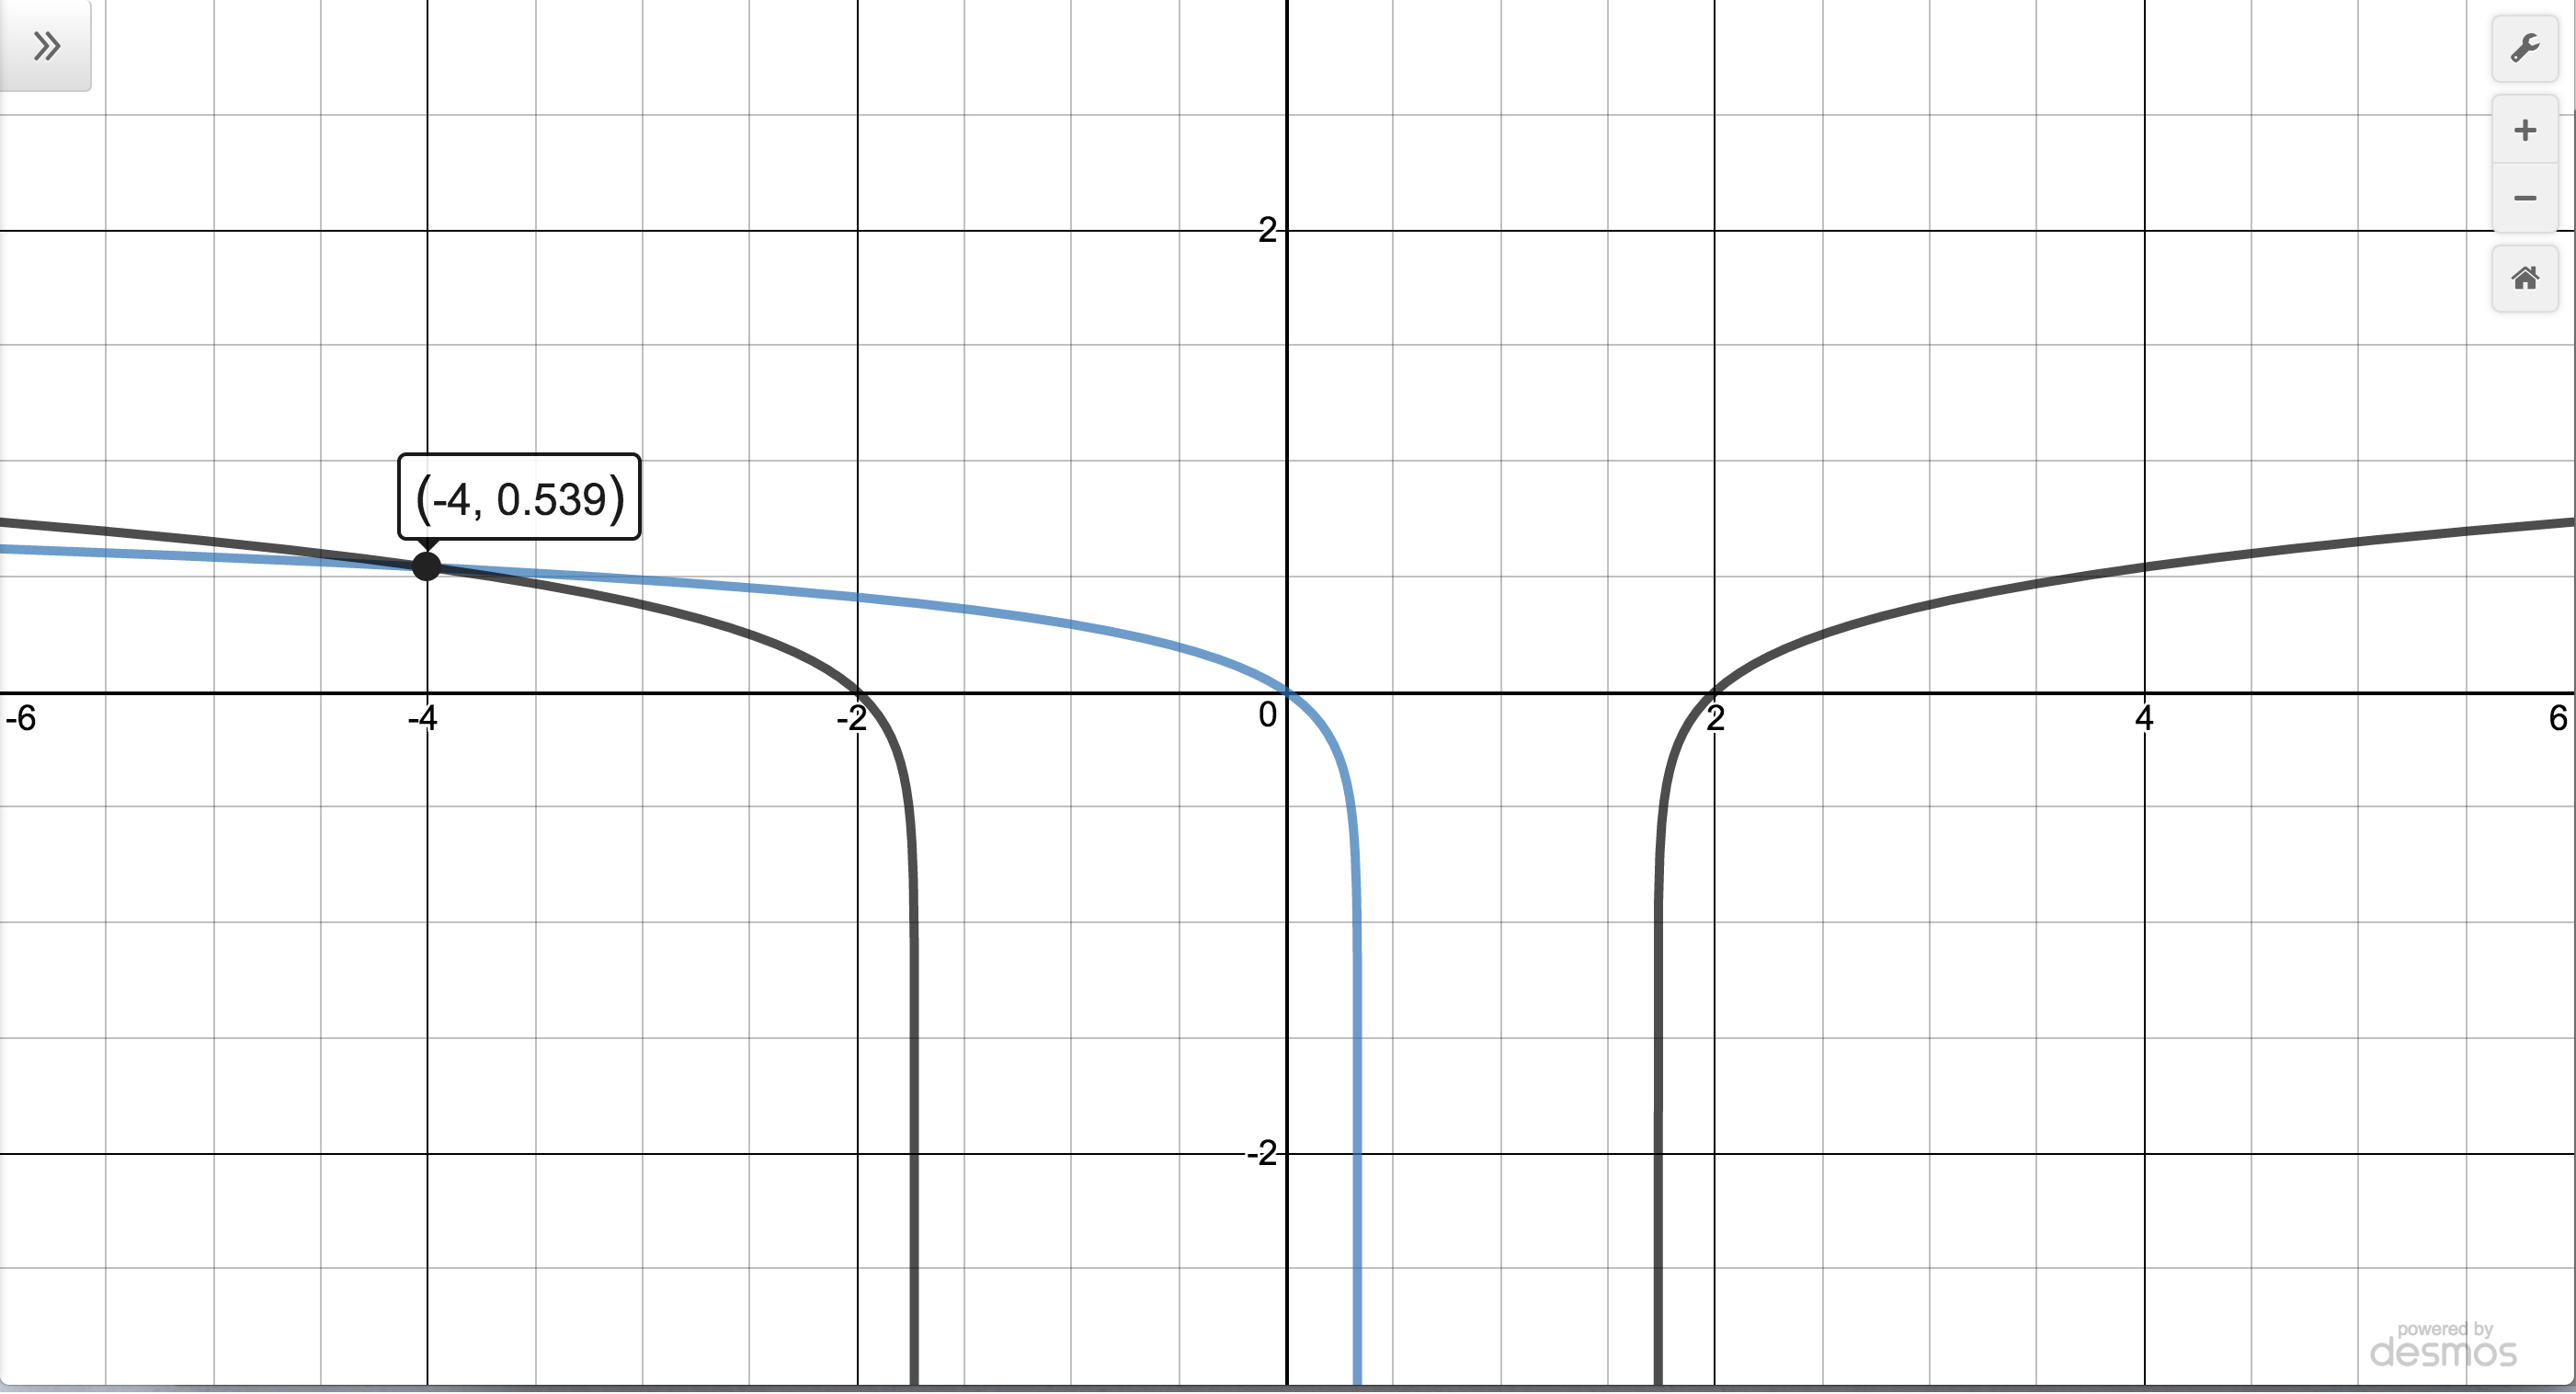
\includegraphics[width=3in]{./LogarithmicEquationsandInequalitiesGraphics/LogEqnEx01.jpg} &

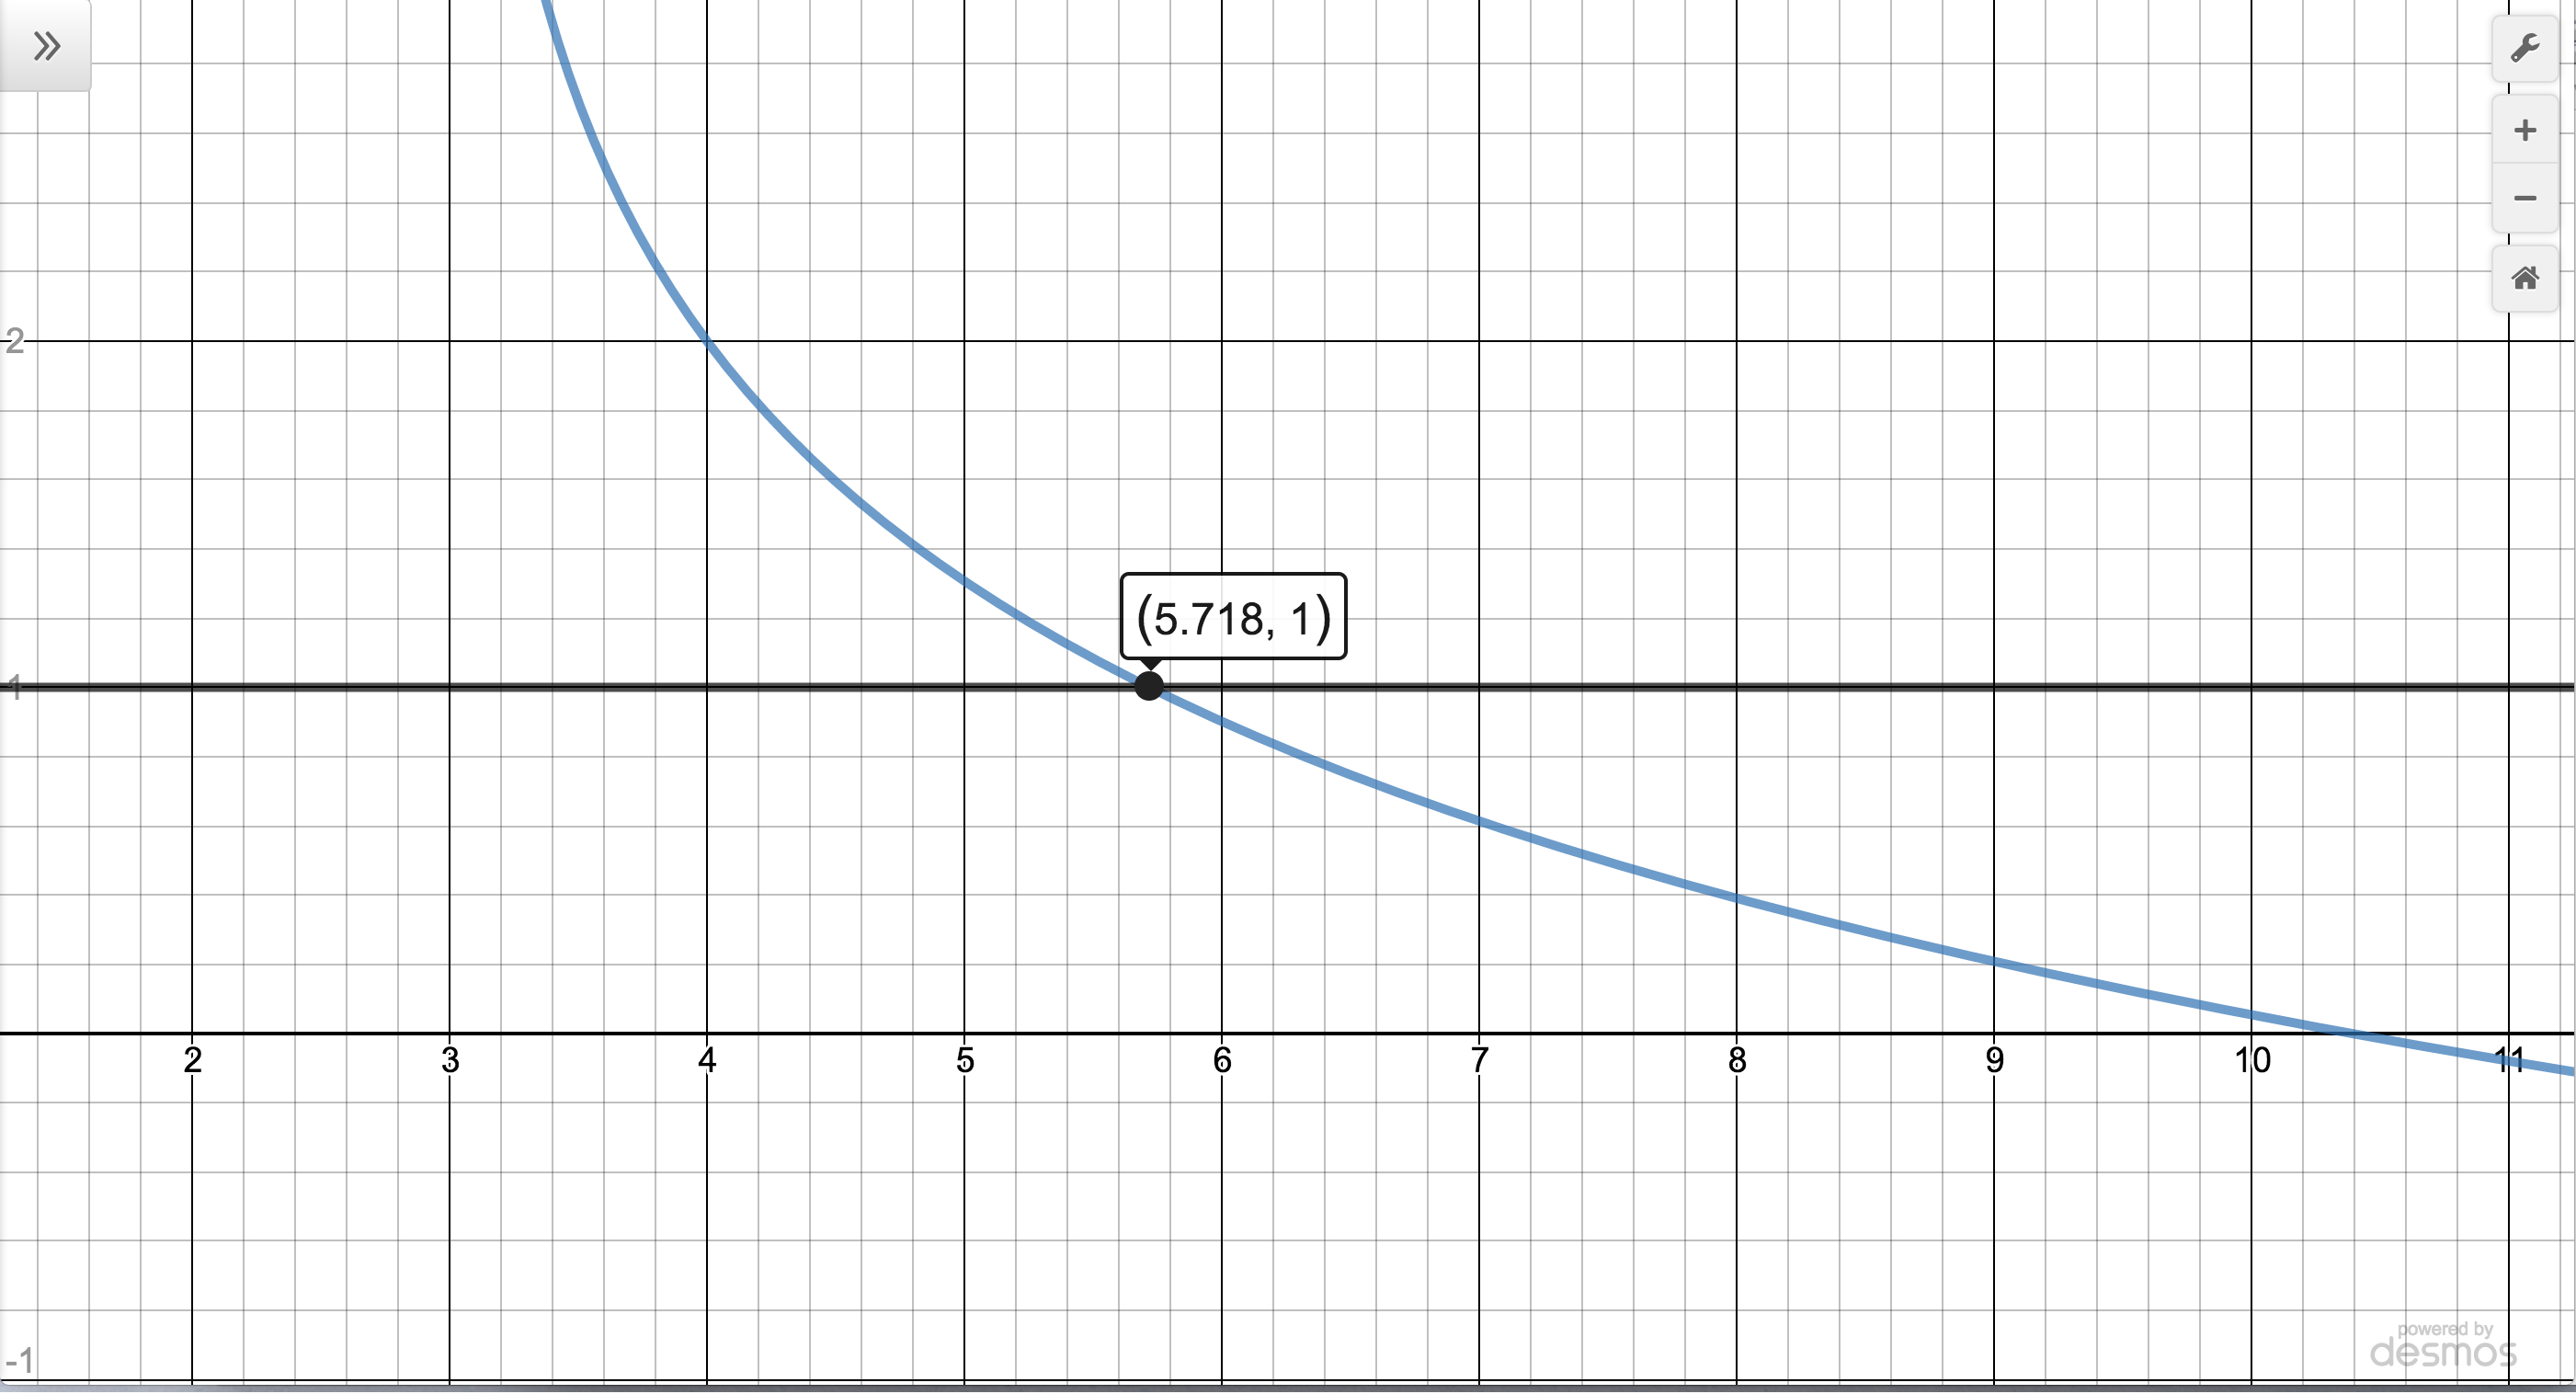
\includegraphics[width=3in]{./LogarithmicEquationsandInequalitiesGraphics/LogEqnEx02.jpg}  \\

Checking $\log_{117}(1-3x) = \log_{117}\left(x^2-3\right)$
 
 &
 
 Checking $2 - \ln(t-3) = 1$
 
\end{tabular}

\end{center}


\item We  start solving $\log_{6}(x+4) + \log_{6}(3-x) = 1$ by using the Product Rule for logarithms to rewrite the equation as  $\log_{6}\left[(x+4)(3-x)\right] = 1$.  

\smallskip

Rewriting as an exponential equation gives $6^{1} = (x+4)(3-x)$ which reduces to $x^2+x-6 = 0$.  We get two solutions: $x=-3$ and $x=2$.   

\smallskip

Using the change of base formula, we graph  $y=f(x) =  \frac{\ln(x+4)}{\ln(6)} + \frac{\ln(3-x)}{\ln(6)}$ and $y=g(x) = 1$ and we see the graphs intersect twice, at $x=-3$ and $x=2$, as required.

\item  Taking a cue from the previous problem, we begin solving $\log_{7}(1-2t) = 1 - \log_{7}(3-t)$ by first collecting the logarithms on the same side, $\log_{7}(1-2t) +  \log_{7}(3-t) = 1$, and then using the Product Rule to get $\log_{7}[(1-2t)(3-t)] = 1$.  

\smallskip

Rewriting  as an exponential equation gives $7^{1} = (1-2t)(3-t)$ which gives the quadratic equation $2t^2-7t-4=0$.  Solving, we find  $t = -\frac{1}{2}$ and $t=4$.  

\smallskip

Once again, we use the change of base formula and find the graphs of  $y = f(t) = \frac{\ln(1-2t)}{\ln(7)}$ and $y=g(t) = 1 - \frac{\ln(3-t)}{\ln(7)}$ intersect only at $t=-\frac{1}{2}$.  

\smallskip

Checking $t=4$ in the original equation produces $\log_{7}(-7) = 1 - \log_{7}(-1)$, showing $t=4$ is not in the domain of $f$ nor $g$.

\begin{center}

\begin{tabular}{cc}

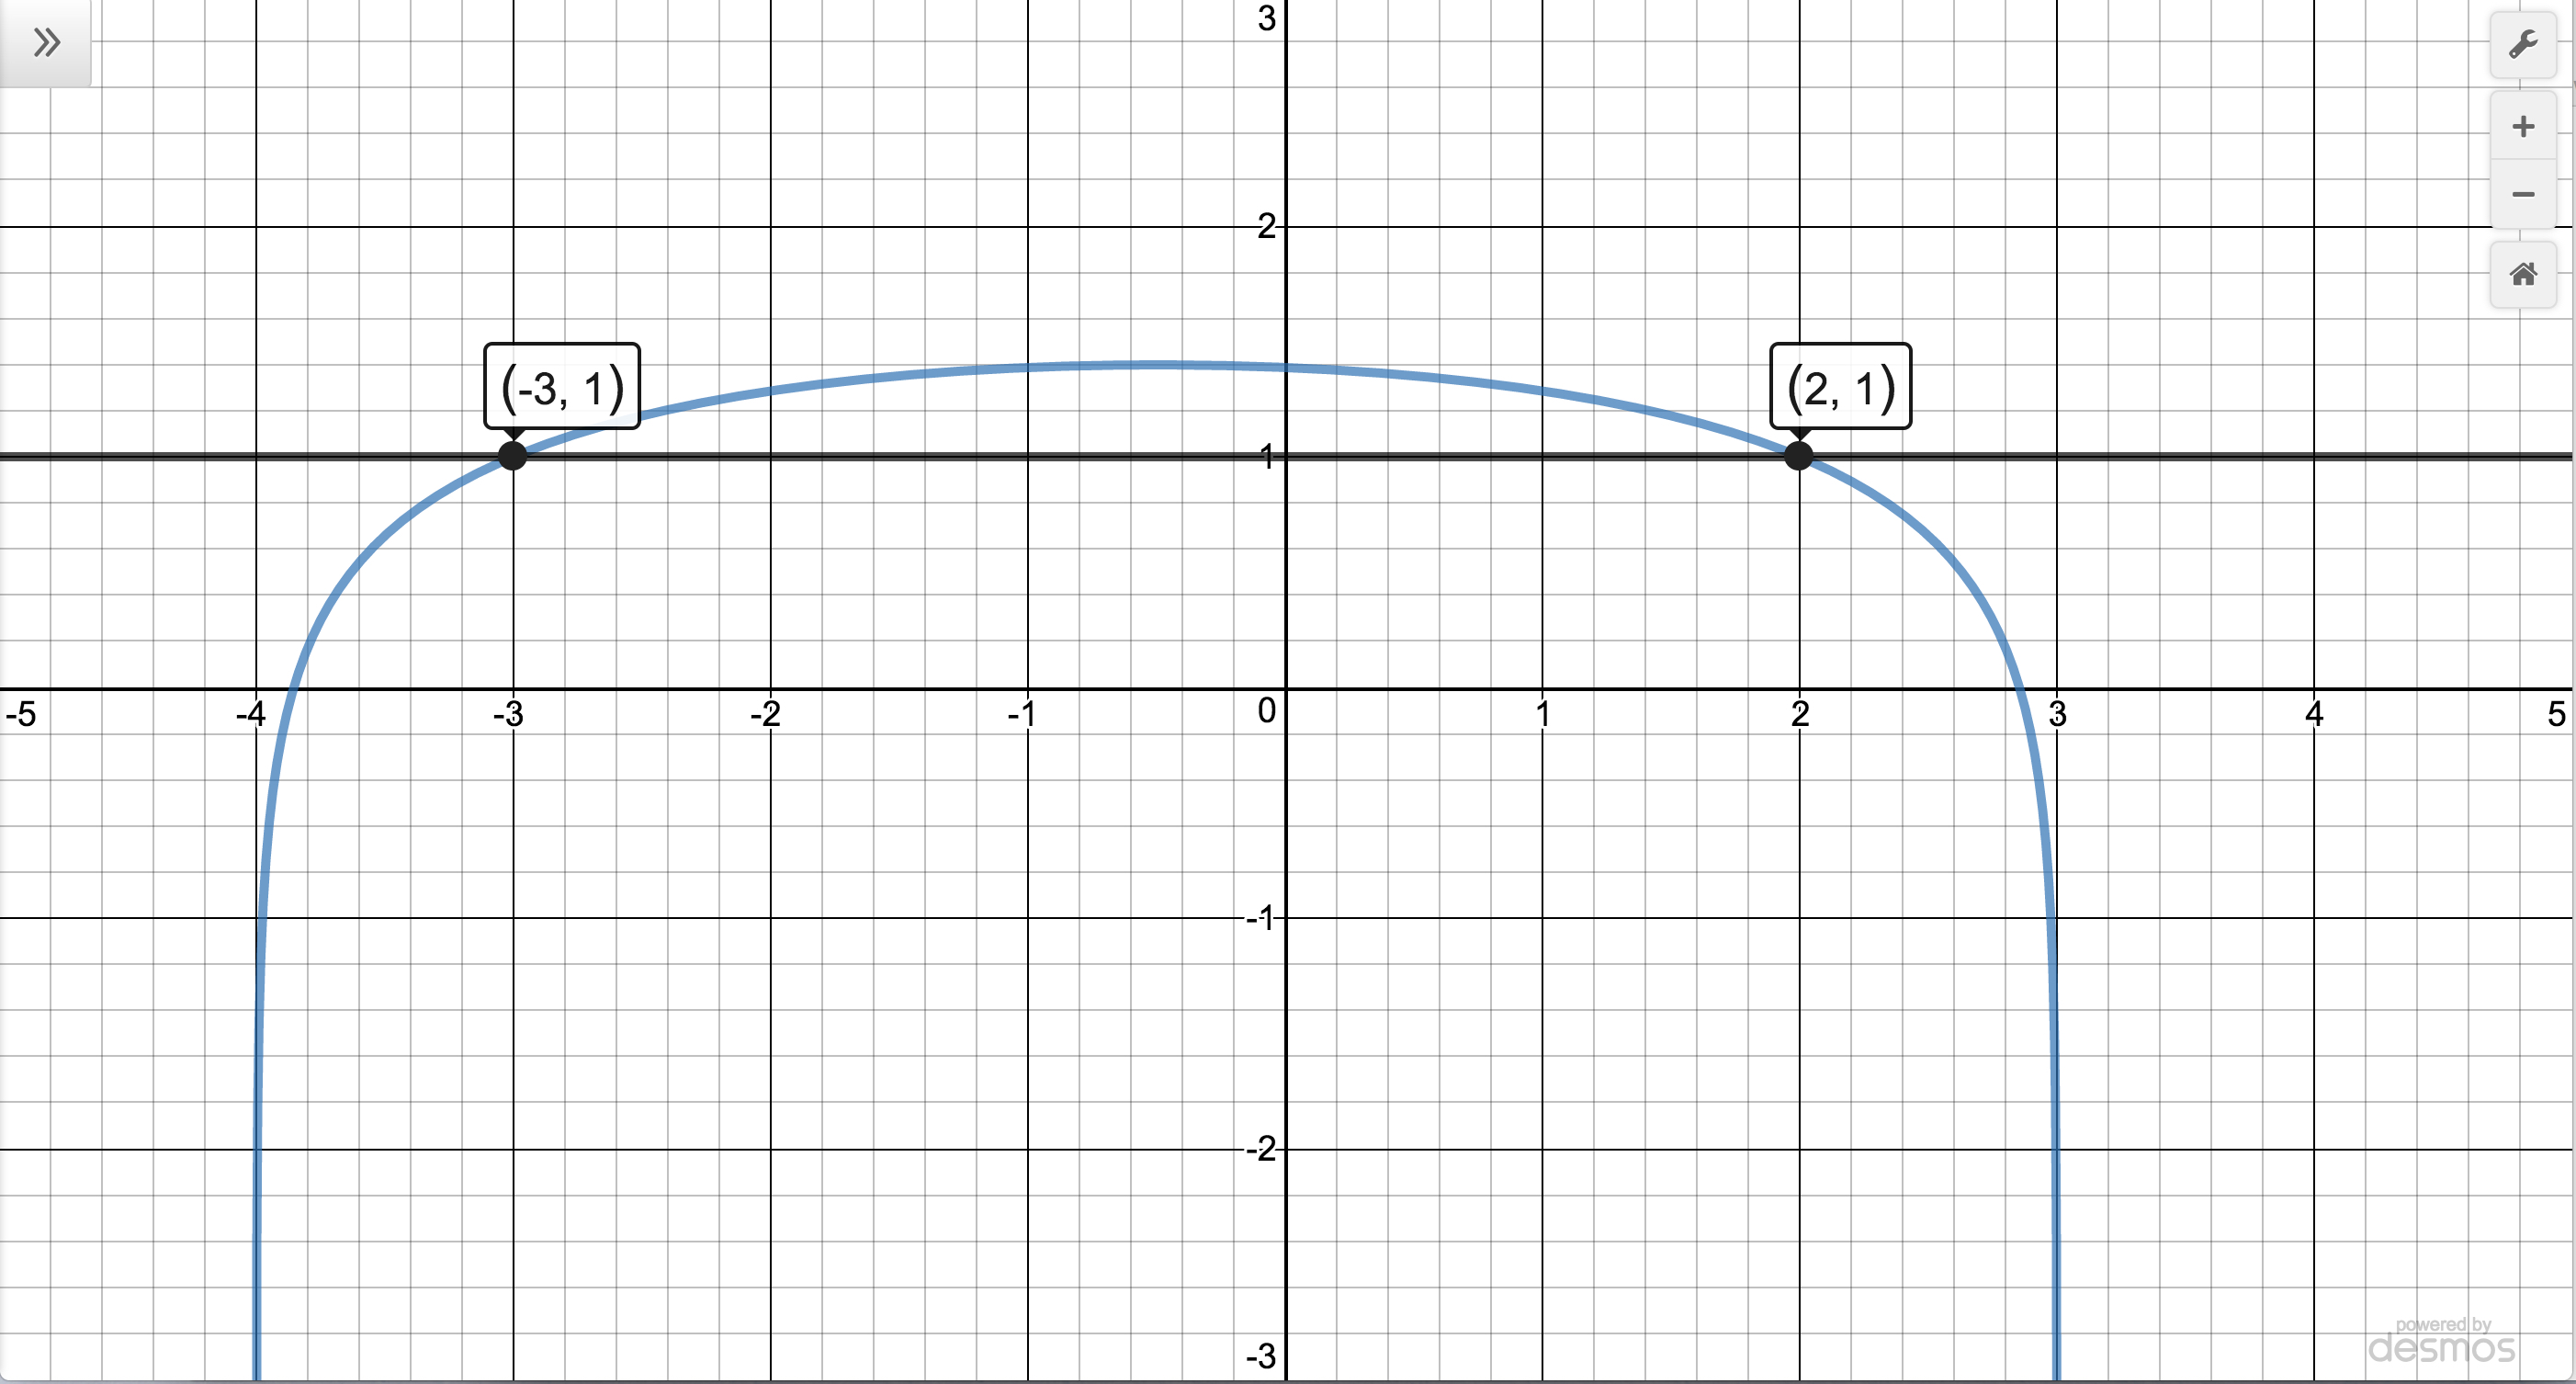
\includegraphics[width=3in]{./LogarithmicEquationsandInequalitiesGraphics/LogEqnEx03.jpg} &

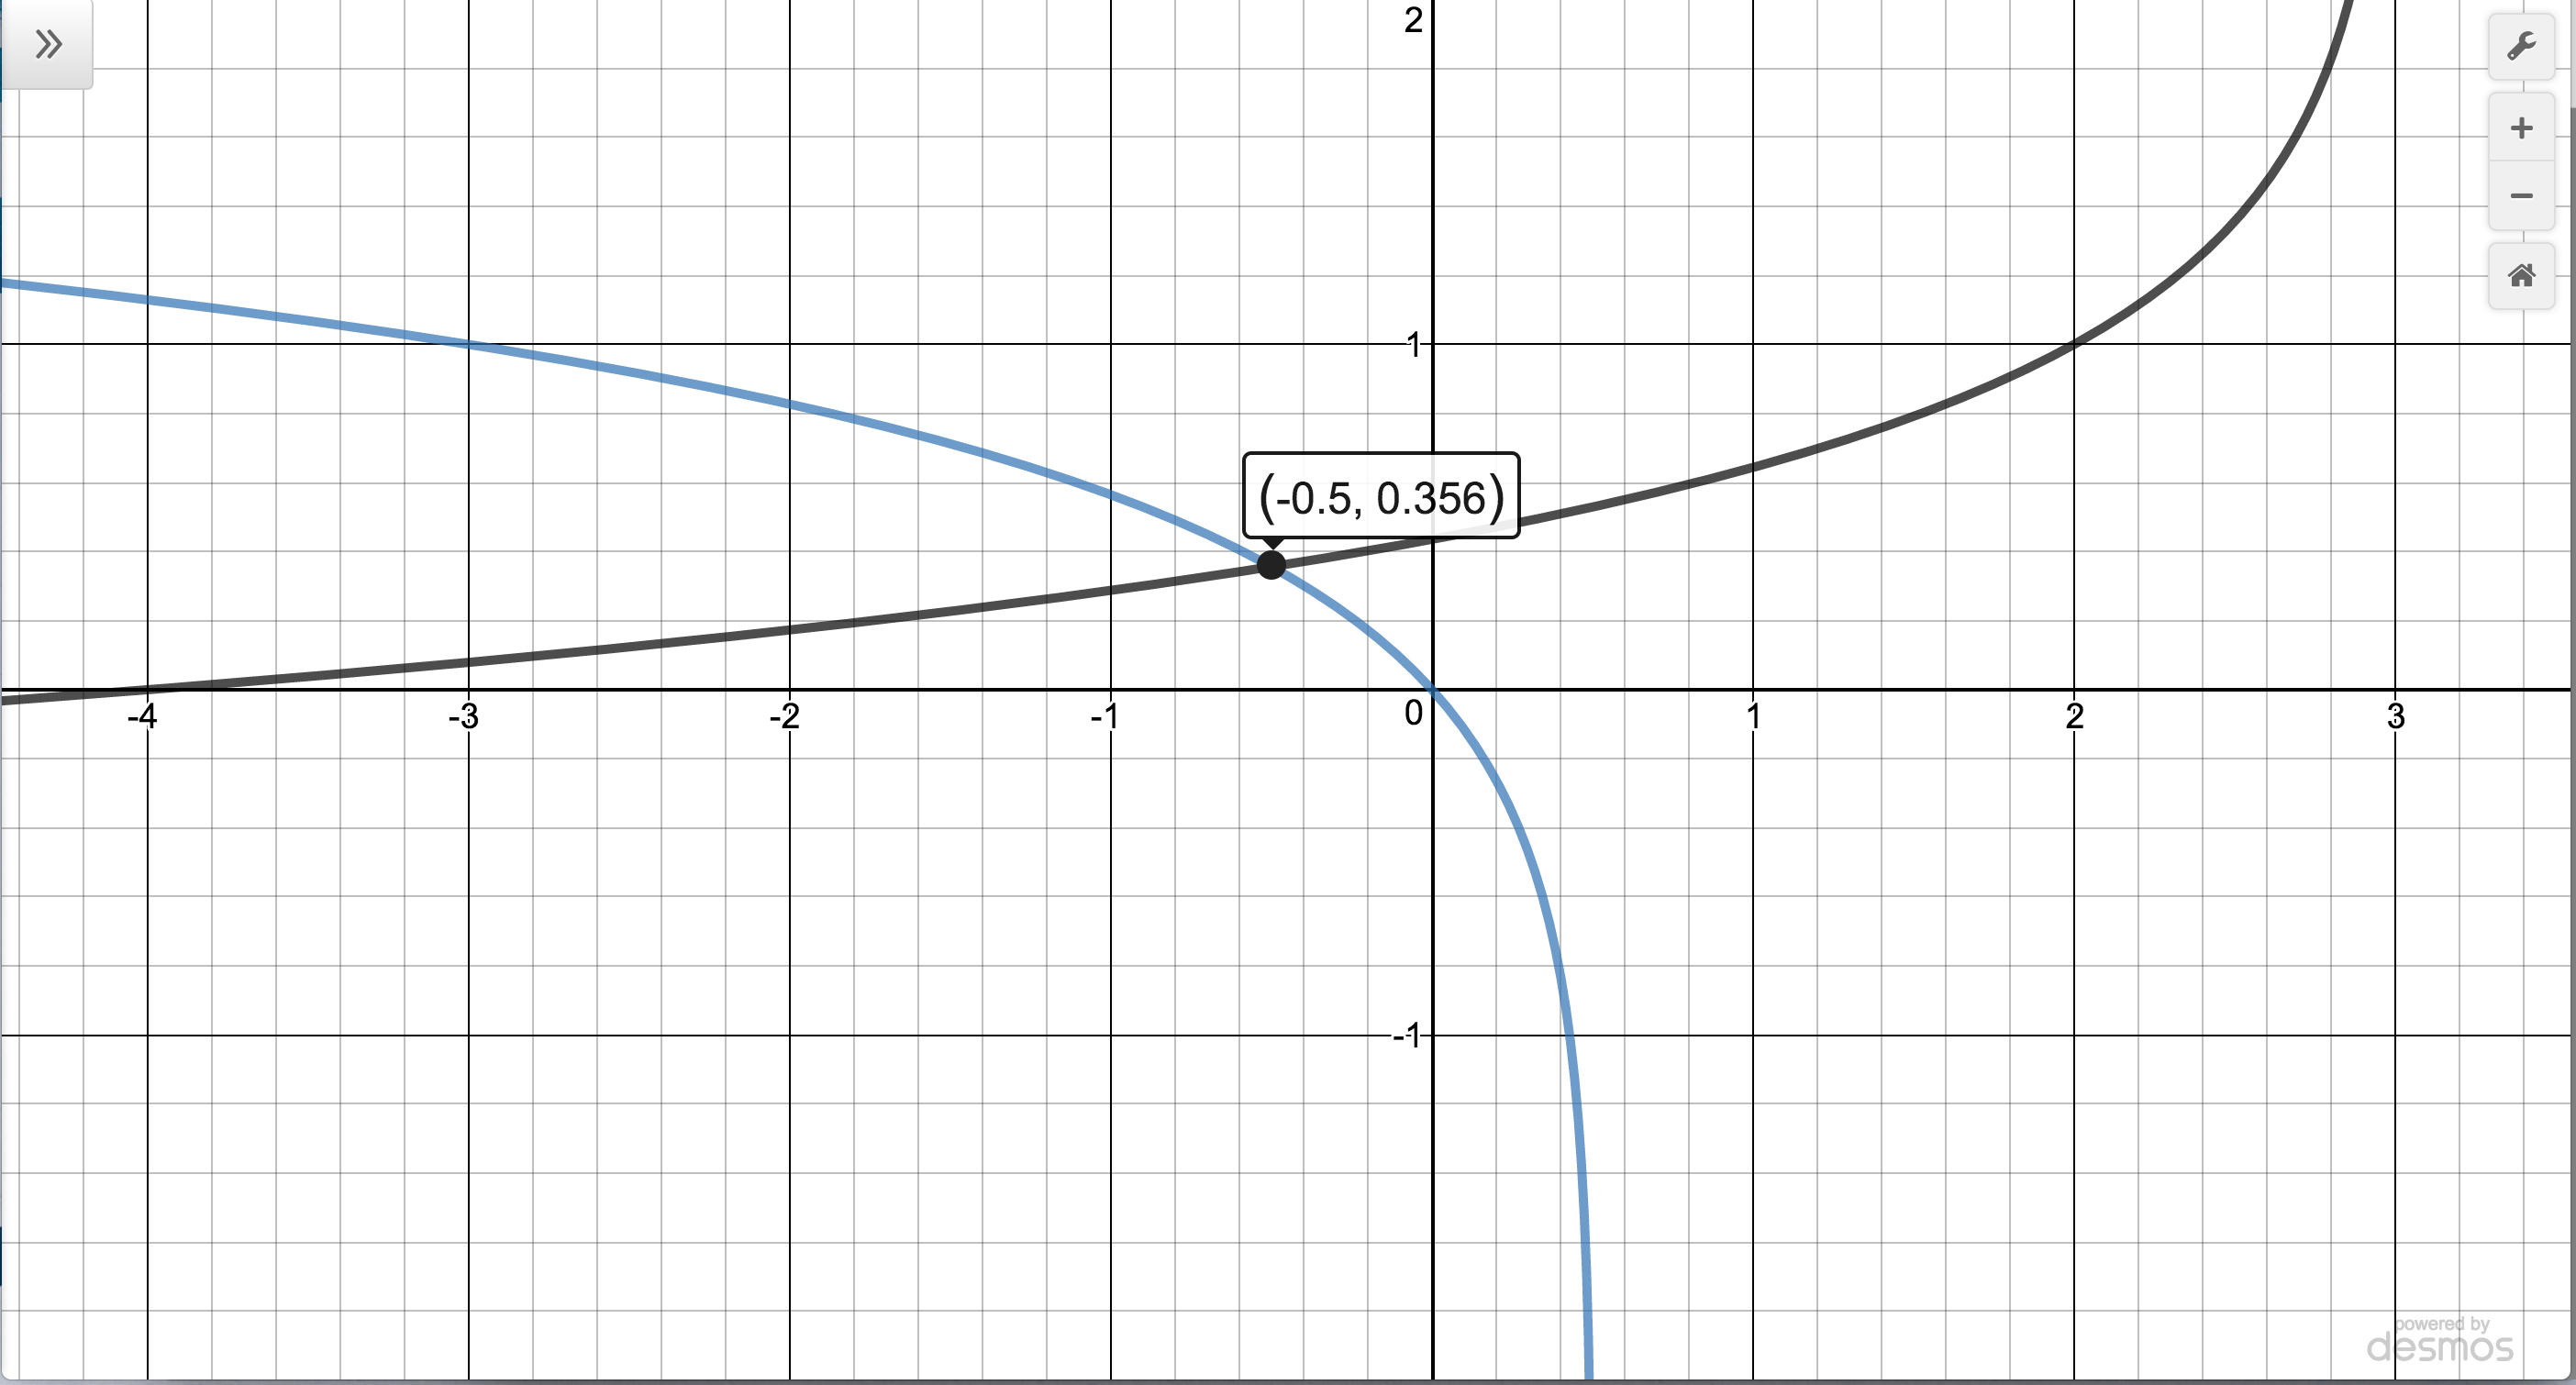
\includegraphics[width=3in]{./LogarithmicEquationsandInequalitiesGraphics/LogEqnEx04.jpg}  \\

Checking $\log_{6}(x+4) + \log_{6}(3-x) = 1$
 
 &
 
 Checking $\log_{7}(1-2t) = 1 - \log_{7}(3-t)$
 
\end{tabular}

\end{center}

\item Our first step in solving  $\log_{2}(x+3) = \log_{2}(6-x)+3$ is to gather the logarithms to one side of of the equation: $\log_{2}(x+3) - \log_{2}(6-x) = 3$.


\smallskip


The  Quotient Rule gives $\log_{2}\left(\frac{x+3}{6-x}\right) = 3$ which, as an exponential equation is $2^{3} = \frac{x+3}{6-x}$. 

\smallskip

Clearing denominators, we get $8(6-x) = x+3$, which reduces to  $x = 5$. 

\smallskip

Using the change of base once again, we graph $f(x) = \frac{\ln(x+3)}{\ln(2)}$ and $g(x) =  \frac{\ln(6-x)}{\ln(2)} + 3$ and find they intersect at $x=5$.


\item Our first step in solving $1 + 2 \log_{4}(t+1) = 2 \log_{2}(t)$ is to gather the logs on one side of the equation.  We obtain  $1 = 2 \log_{2}(t) - 2 \log_{4}(t+1)$ but find we need a common base to combine the logs.

\smallskip

Since $4$ is a power of $2$, we use change of base to convert  $\log_{4}(t+1) = \frac{\log_{2}(t+1)}{\log_{2}(4)} = \frac{1}{2} \log_{2}(t+1)$.  Hence, our original equation becomes  

\[ \begin{array}{rclr}

1 & = & 2 \log_{2}(t) - 2 \left(\frac{1}{2} \log_{2}(t+1)\right) & \\ [2pt]
1 &= & 2\log_{2}(t) - \log_{2}(t+1) & \\ [2pt]
1 & = & \log_{2}\left(t^2\right) - \log_{2}(t+1) & \text{Power Rule} \\ [6pt]
1 & = & \log_{2}\left( \dfrac{t^{2}}{t+1}\right) & \text{Quotient Rule} \\ \end{array}\]

Rewriting $1 = \log_{2}\left( \frac{t^{2}}{t+1}\right)$ in exponential form gives  $ \frac{t^{2}}{t+1} = 2$ or $t^2 -2t-2 = 0$.  Using the quadratic formula, we obtain  $t = 1 \pm \sqrt{3}$.

One last time, we use the change of base formula and graph  $f(t) = 1 + \frac{2\ln(t+1)}{\ln(4)}$ and $g(t) = \frac{2 \ln(t)}{\ln(2)}$.   We see the graphs intersect only at $t \approx 2.732 \approx 1 + \sqrt{3}$.  

\smallskip

Note the solution $t = 1 - \sqrt{3} < 0$ Hence if substituted into the original equation, the term $2 \log_{2}\left(1 - \sqrt{3}\right)$ is undefined, which explains why the graphs below intersect only once.

\begin{center}

\begin{tabular}{cc}

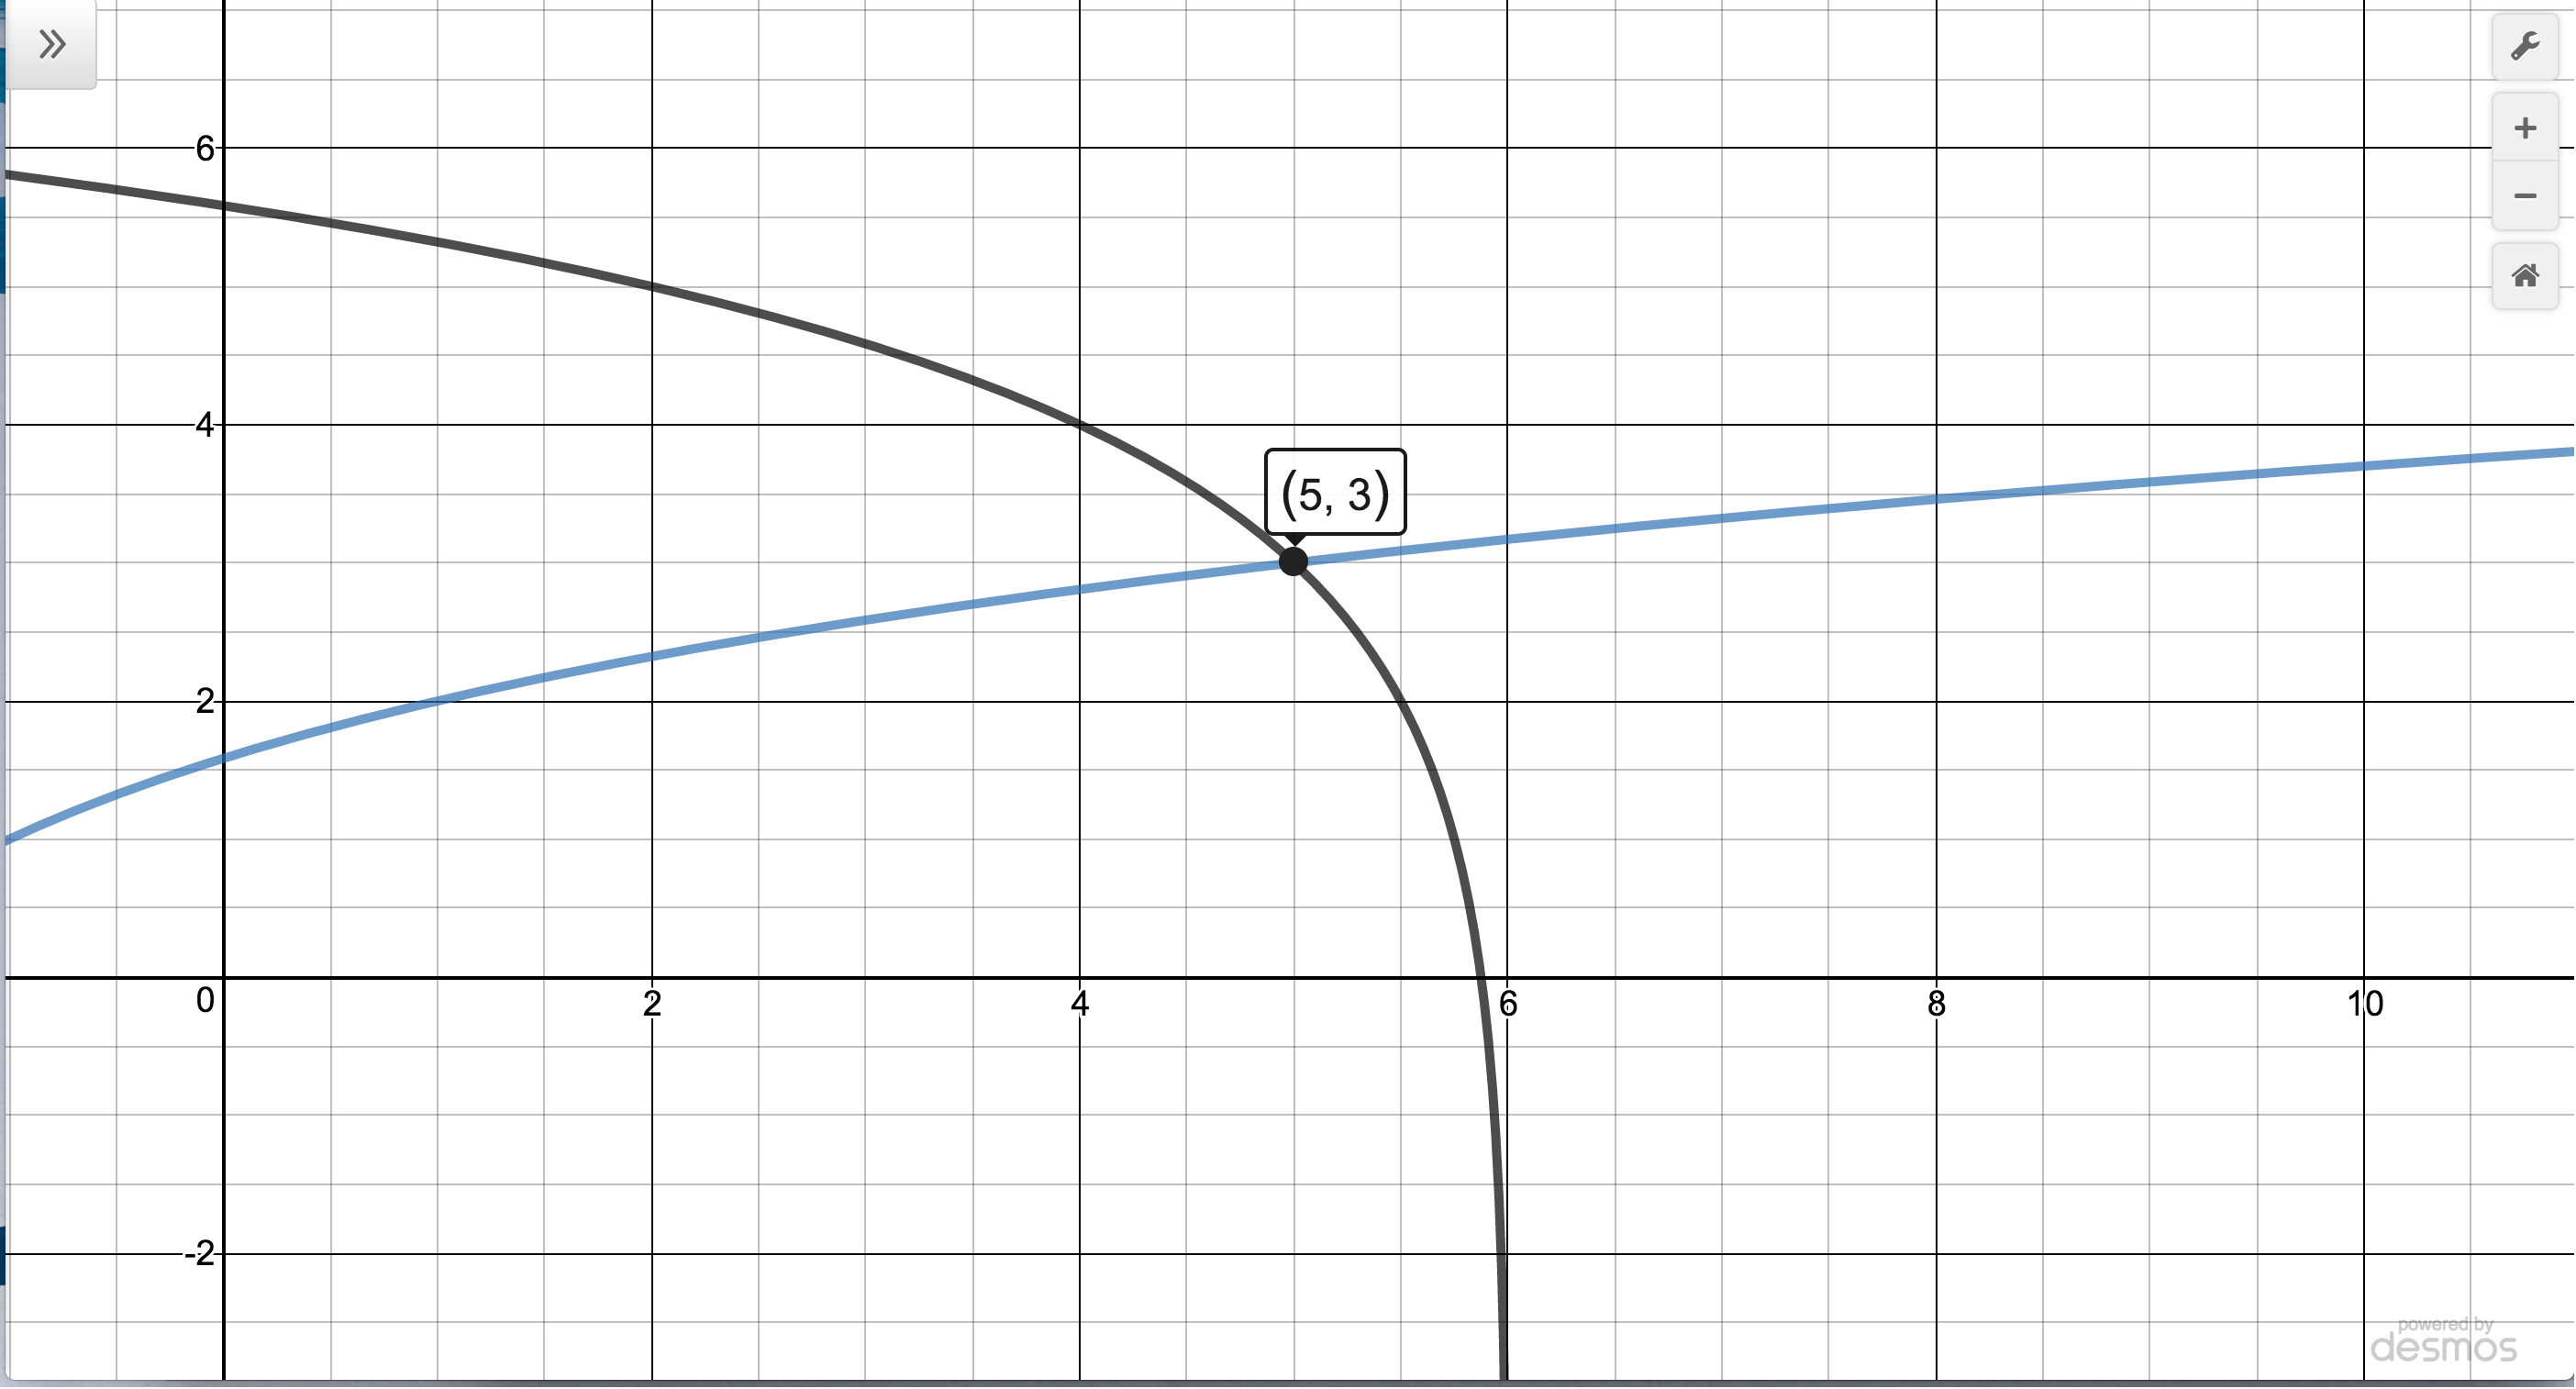
\includegraphics[width=3in]{./LogarithmicEquationsandInequalitiesGraphics/LogEqnEx05.jpg} &

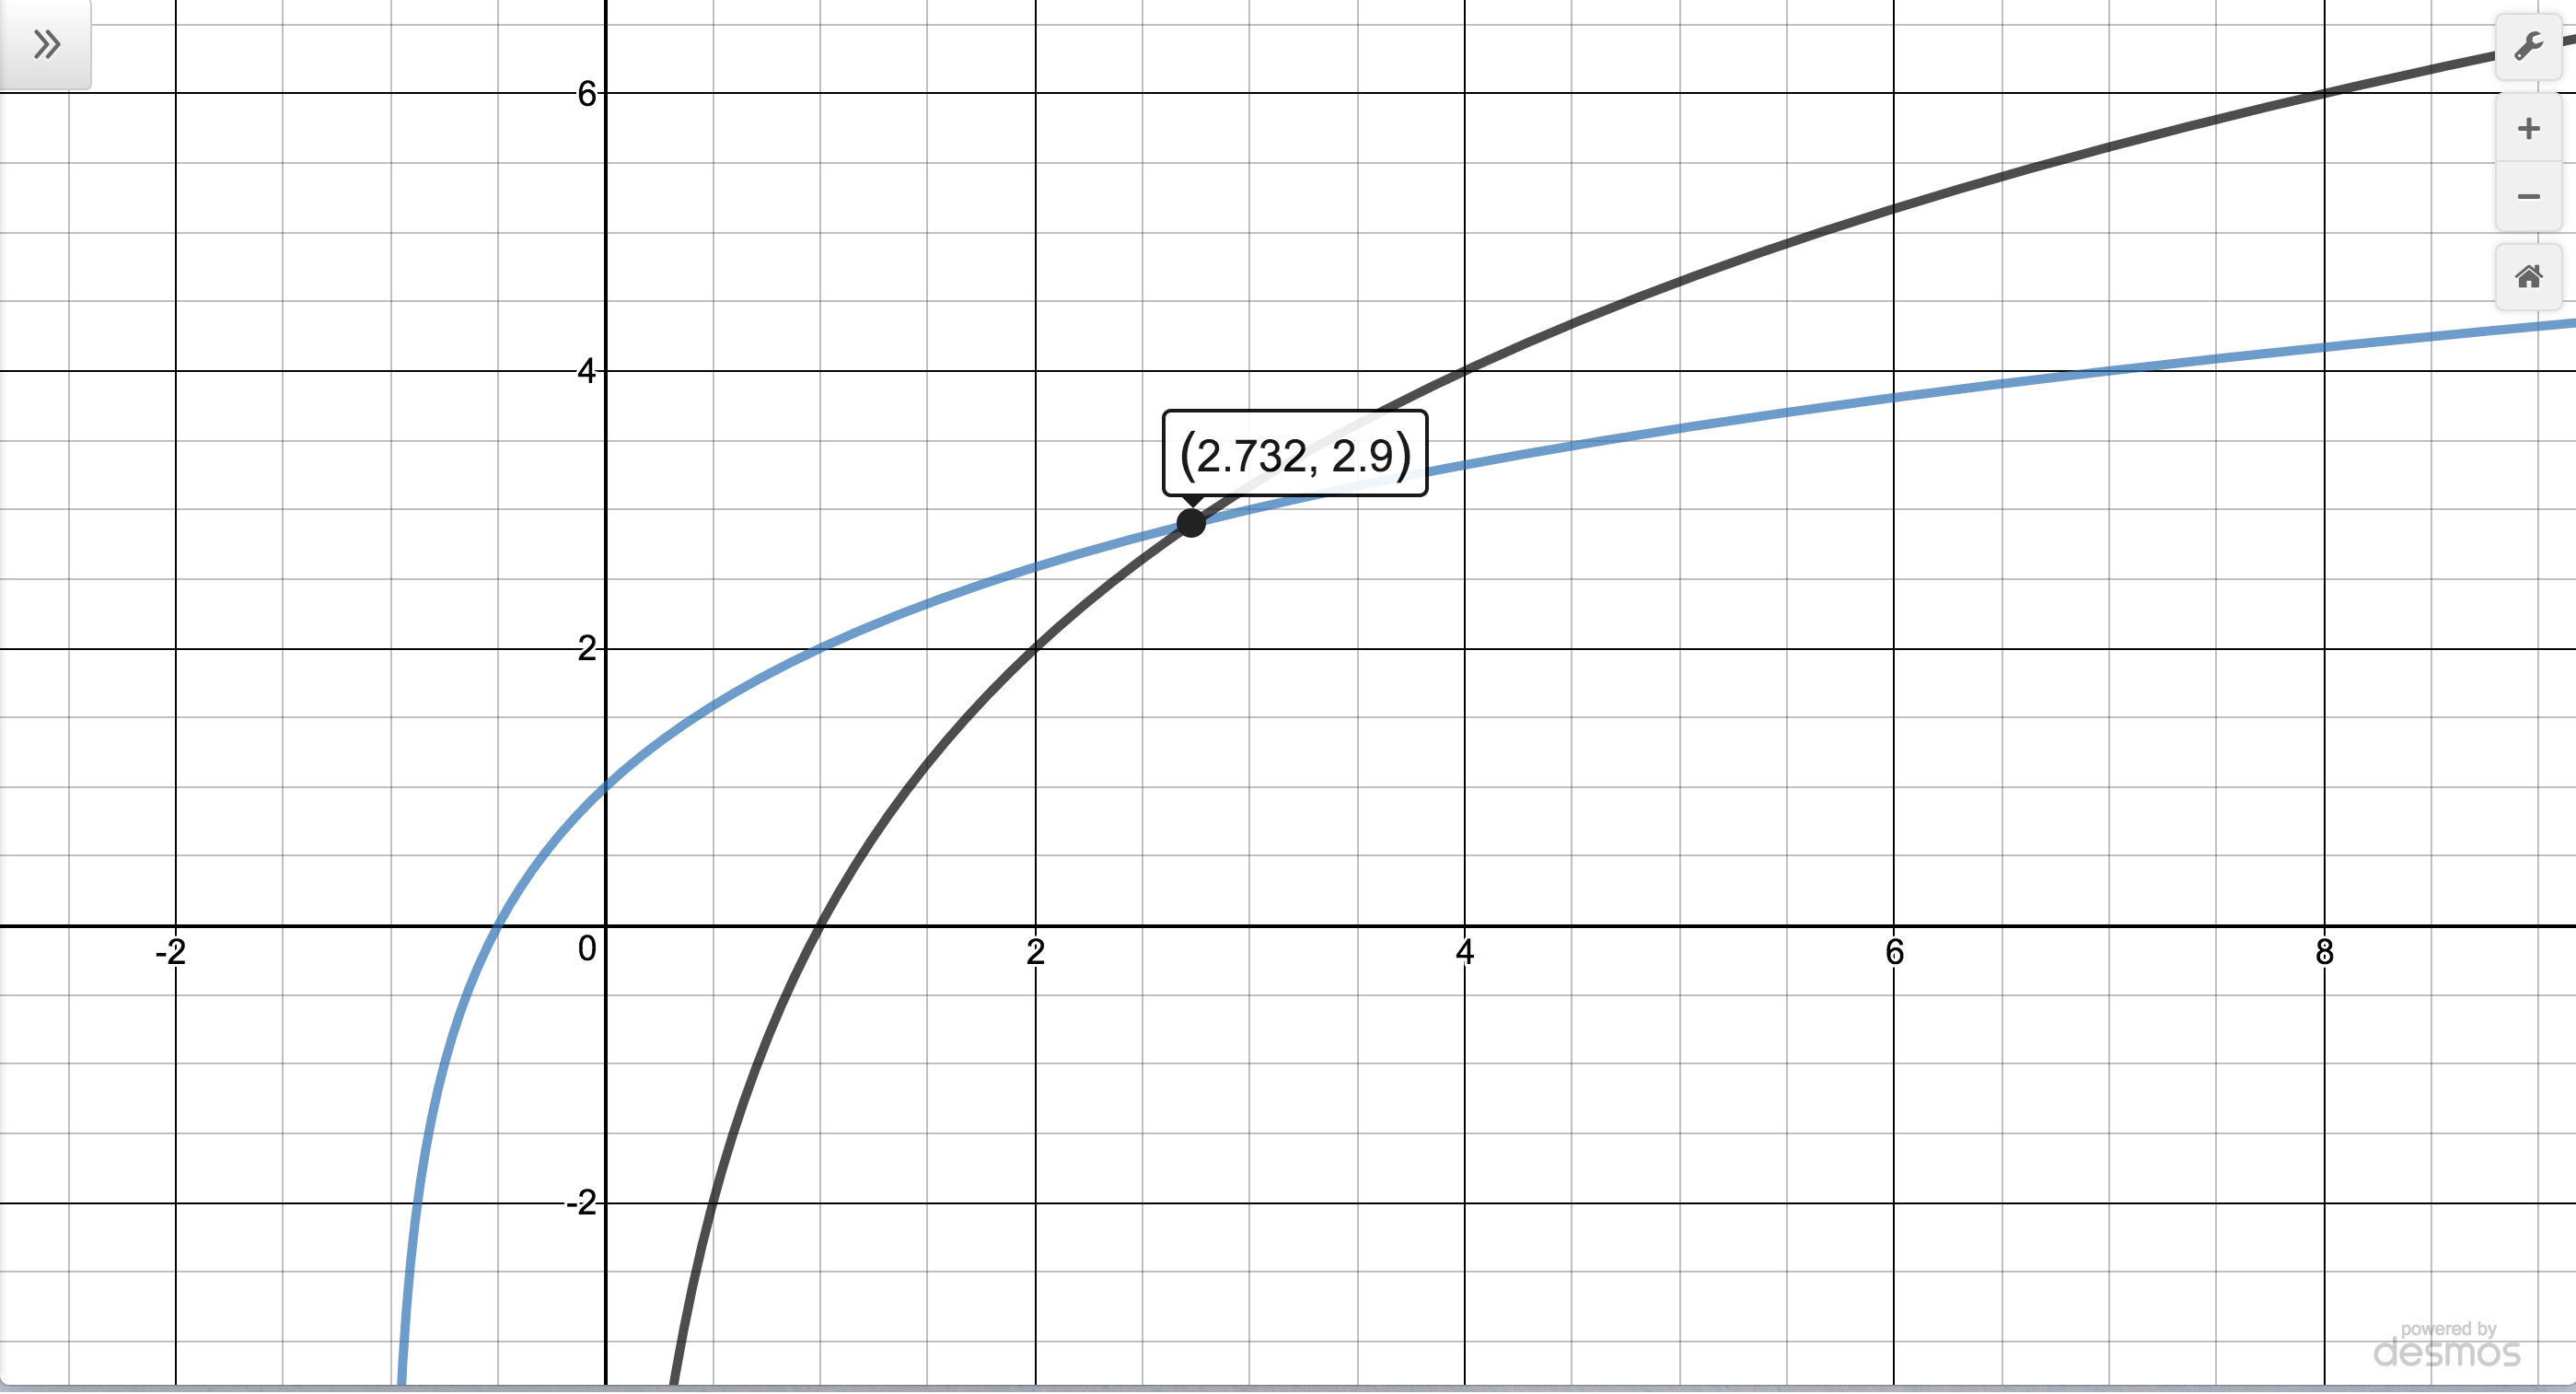
\includegraphics[width=3in]{./LogarithmicEquationsandInequalitiesGraphics/LogEqnEx06.jpg}  \\

Checking $\log_{2}(x+3) = \log_{2}(6-x)+3$
 
 &
 
 Checking $1 + 2 \log_{4}(t+1) = 2 \log_{2}(t)$
 
\end{tabular}

\end{center}
\end{enumerate}

\qed
\end{ex}

If nothing else,  Example \ref{LogEqnsEx1} demonstrates the importance of checking for extraneous solutions\footnote{Recall that an extraneous solution is an answer obtained analytically which does not satisfy the original equation.} when solving equations involving logarithms.  Even though we checked our answers graphically, extraneous solutions are easy to spot:  any supposed solution which causes the argument of a logarithm to be negative must be discarded.  

\smallskip

While identifying extraneous solutions is important, it is equally important to understand which machinations create the opportunity for extraneous solutions to appear.  In the case of Example \ref{LogEqnsEx1}, extraneous solutions, by and large, result from using the Power, Product, or Quotient Rules.  We encourage the reader to take the time to track each extraneous solution found in  Example \ref{LogEqnsEx1}  backwards through the solution process to see at precisely which step it fails to be a solution.

\smallskip

As with the equations in Example \ref{expeqnsex1}, much can be learned from checking all of the answers in Example \ref{LogEqnsEx1} analytically.  We leave this to the reader and turn our attention to inequalities involving logarithmic functions.  Since logarithmic functions are continuous on their domains, we can use sign diagrams.  

\smallskip
\begin{comment}
\begin{ex}  Solve the following inequalities.  Check your answer graphically using a calculator.
\label{logineq}

\begin{multicols}{3}

\begin{enumerate}

\item  $\dfrac{1}{\ln(x)+1} \leq 1$

\item  $\left(\log_{2}(x)\right)^2 < 2 \log_{2}(x) + 3$

\item  $t \log(t+1) \geq t$


\end{enumerate}

\end{multicols}


{\bf Solution.}  

\begin{enumerate}

\item  We start solving $\frac{1}{\ln(x)+1} \leq 1$ by getting $0$ on one side of the inequality: $\frac{1}{\ln(x)+1}  - 1 \leq 0$.  

\smallskip

Getting a common denominator yields $\frac{1}{\ln(x)+1}  - \frac{\ln(x)+1}{\ln(x)+1} \leq 0$ which reduces to $\frac{-\ln(x)}{\ln(x)+1} \leq 0$, or $ \frac{\ln(x)}{\ln(x)+1} \geq 0$.  

\smallskip

We define $r(x) = \frac{\ln(x)}{\ln(x)+1}$ and set about finding the domain and the zeros of $r$.  Due to the appearance of the term $\ln(x)$, we require  $x > 0$.  In order to keep the denominator away from zero, we solve $\ln(x)+1 = 0$ so $\ln(x) = -1$, so $x = e^{-1} = \frac{1}{e}$.  Hence, the domain of $r$ is $\left(0, \frac{1}{e}\right) \cup \left(\frac{1}{e}, \infty\right)$. 

\smallskip

To find the zeros of $r$, we set $r(x) = \frac{\ln(x)}{\ln(x)+1} = 0$ so that $\ln(x) = 0$, and we find $x = e^{0} = 1$.  


\smallskip

In order to determine test values for $r$ without resorting to the calculator, we need to find numbers between $0$, $\frac{1}{e}$, and $1$ which have a base of $e$.  Since $e \approx 2.718 > 1$, $0 < \frac{1}{e^2} < \frac{1}{e} < \frac{1}{\sqrt{e}} < 1 < e$.  

\smallskip

To determine the sign of $r\left( \frac{1}{e^2} \right)$, note $\ln\left(\frac{1}{e^2}\right) = \ln\left(e^{-2}\right) = -2$. Hence, $r\left( \frac{1}{e^2} \right) = \frac{-2}{-2+1} = 2 > 0$.  The rest of the test values are determined similarly.   


\smallskip

From our sign diagram, we find $r(x) \geq 0$ on $\left(0, \frac{1}{e}\right) \cup [1, \infty)$, which is our solution. 


\smallskip

Graphing $f(x) =  \frac{1}{\ln(x)+1}$ and $g(x) = 1$, we see the graph of $f$ is below the graph of $g$ on these intervals, and that the graphs intersect at $x=1$.

\begin{center}

\begin{tabular}{cc}

\begin{mfpic}[10]{-6}{6}{-2}{2}
\arrow \polyline{(-6,0),(6,0)}
\xmarks{-2,2}
\scriptsize
\tlpointsep{6pt}
\normalsize
\tlabel[cc](-6,-1){$0$}
\tlabel[cc](-4,1){$(+)$}
\tlabel[cc](-2,-1){$\frac{1}{e}$}
\tlabel[cc](-2,1){\textinterrobang}
\tlabel[cc](0,1){$(-)$}
\tlabel[cc](2,-1){$1$}
\tlabel[cc](2,1){$0$}
\tlabel[cc](4,1){$(+)$}
\pointfillfalse
\point[4pt]{(-6,0)}
\end{mfpic} 

& 

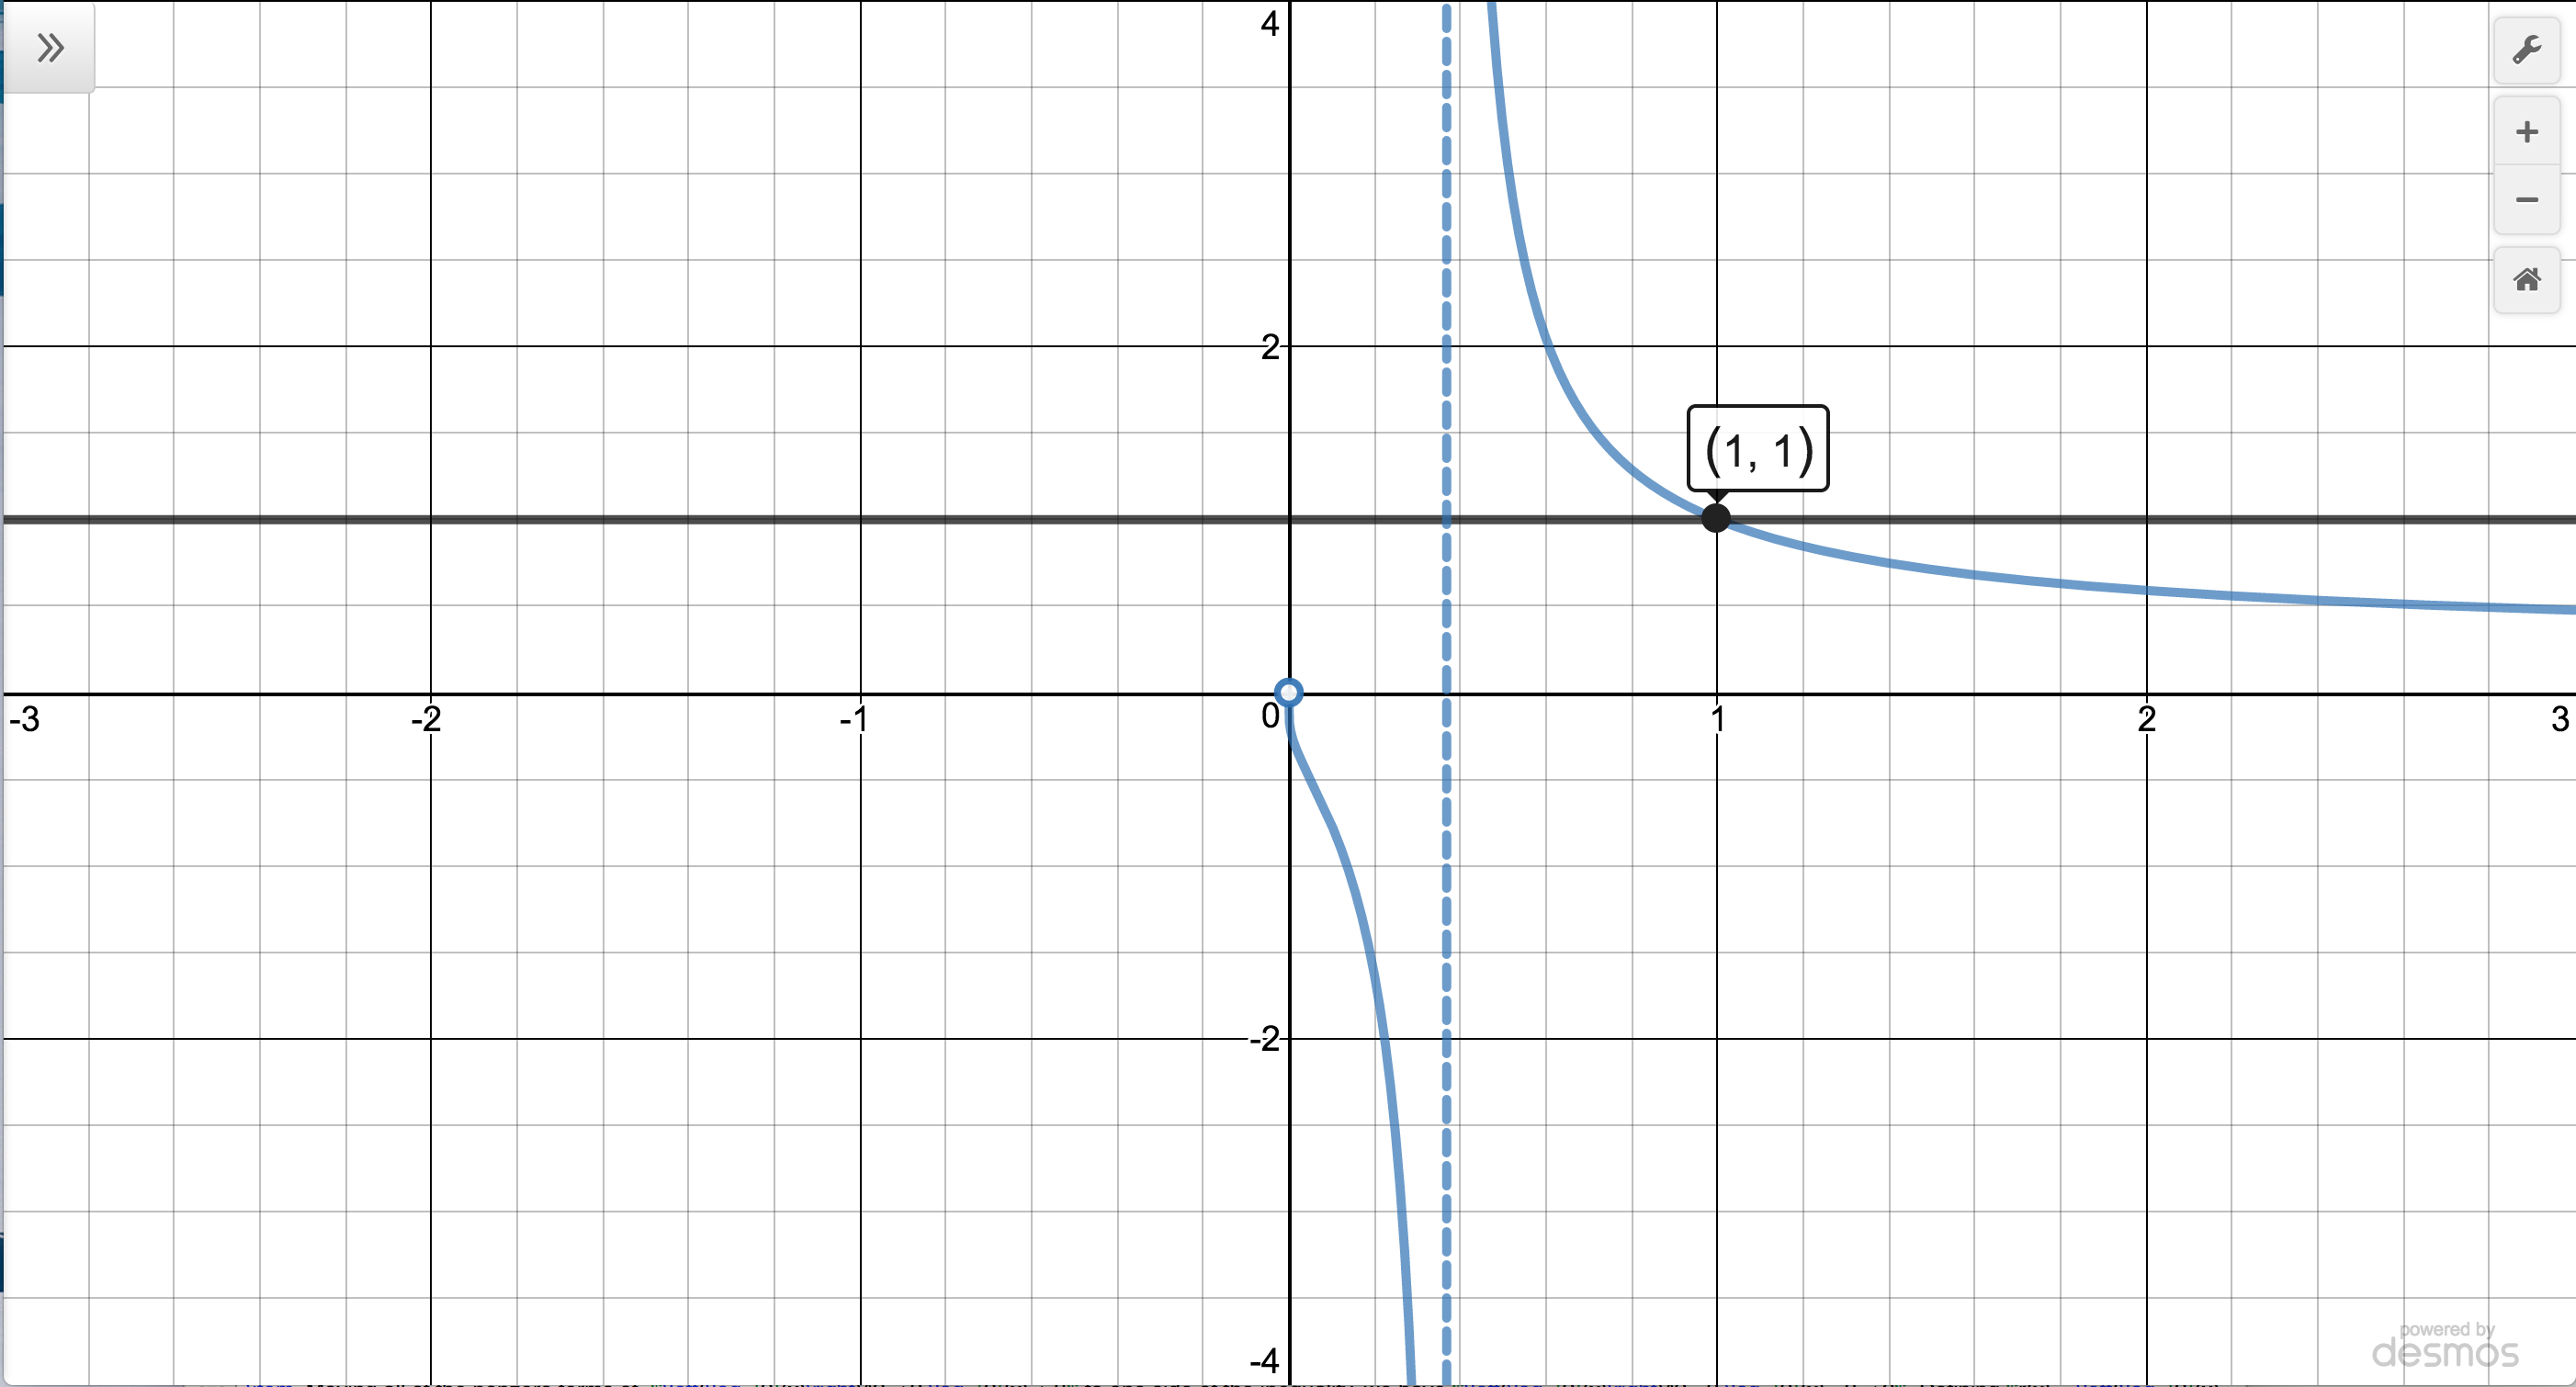
\includegraphics[width=3in]{./LogarithmicEquationsandInequalitiesGraphics/LogEqnEx07.jpg} \\

A sign diagram for $r(x) = \dfrac{\ln(x)}{\ln(x)+1}$

&

Checking  $\dfrac{1}{\ln(x)+1} \leq 1$



\end{tabular}

\end{center}


\item  Moving all of the nonzero terms of  $\left(\log_{2}(x)\right)^2 < 2 \log_{2}(x) + 3$ to one side of the inequality in order to make use of a sign diagram, we have $\left(\log_{2}(x)\right)^2 - 2 \log_{2}(x) - 3 < 0$. 

\smallskip

Defining $r(x) = \left(\log_{2}(x)\right)^2 - 2 \log_{2}(x) - 3$, we get the domain of $r$ is $(0, \infty)$, due to the presence of the logarithm.  To find the zeros of $r$, we set $r(x) =\left(\log_{2}(x)\right)^2 - 2 \log_{2}(x) - 3= 0$ which we identify as a  `quadratic in disguise.'  

\smallskip

Setting $u = \log_{2}(x)$, our equation becomes $u^2-2u-3 = 0$.  Factoring   gives us $u=-1$ and $u=3$.  Since $u = \log_{2}(x)$, we get $\log_{2}(x) = -1$, or $x = 2^{-1} = \frac{1}{2}$, and $\log_{2}(x) = 3$, which gives  $x = 2^{3} = 8$.  

\smallskip

We use test values which are powers of $2$: $0 < \frac{1}{4} < \frac{1}{2} < 1 < 8 < 16$ to create the sign diagram below.  From our sign diagram, we see $r(x)< 0$, which corresponds to our solution,  on $\left(\frac{1}{2}, 8 \right)$. 

\smallskip

Geometrically, the graph of $f(x)= \left(\frac{\ln(x)}{\ln(2)}\right)^2$ is below the graph of $y = g(x) = \frac{2 \ln(x)}{\ln(2)} + 3$ on $\left(\frac{1}{2}, 8 \right)$.

\begin{center}

\begin{tabular}{m{2in}c}

\begin{mfpic}[10]{-6}{6}{-2}{2}
\arrow \polyline{(-6,0),(6,0)}
\xmarks{-2,2}
\scriptsize
\tlpointsep{6pt}
\normalsize
\tlabel[cc](-6,-1){$0$}
\tlabel[cc](-4,1){$(+)$}
\tlabel[cc](-2,-1){$\frac{1}{2}$}
\tlabel[cc](-2,1){$0$}
\tlabel[cc](0,1){$(-)$}
\tlabel[cc](2,-1){$8$}
\tlabel[cc](2,1){$0$}
\tlabel[cc](4,1){$(+)$}
\pointfillfalse
\point[4pt]{(-6,0)}
\end{mfpic} 

& 

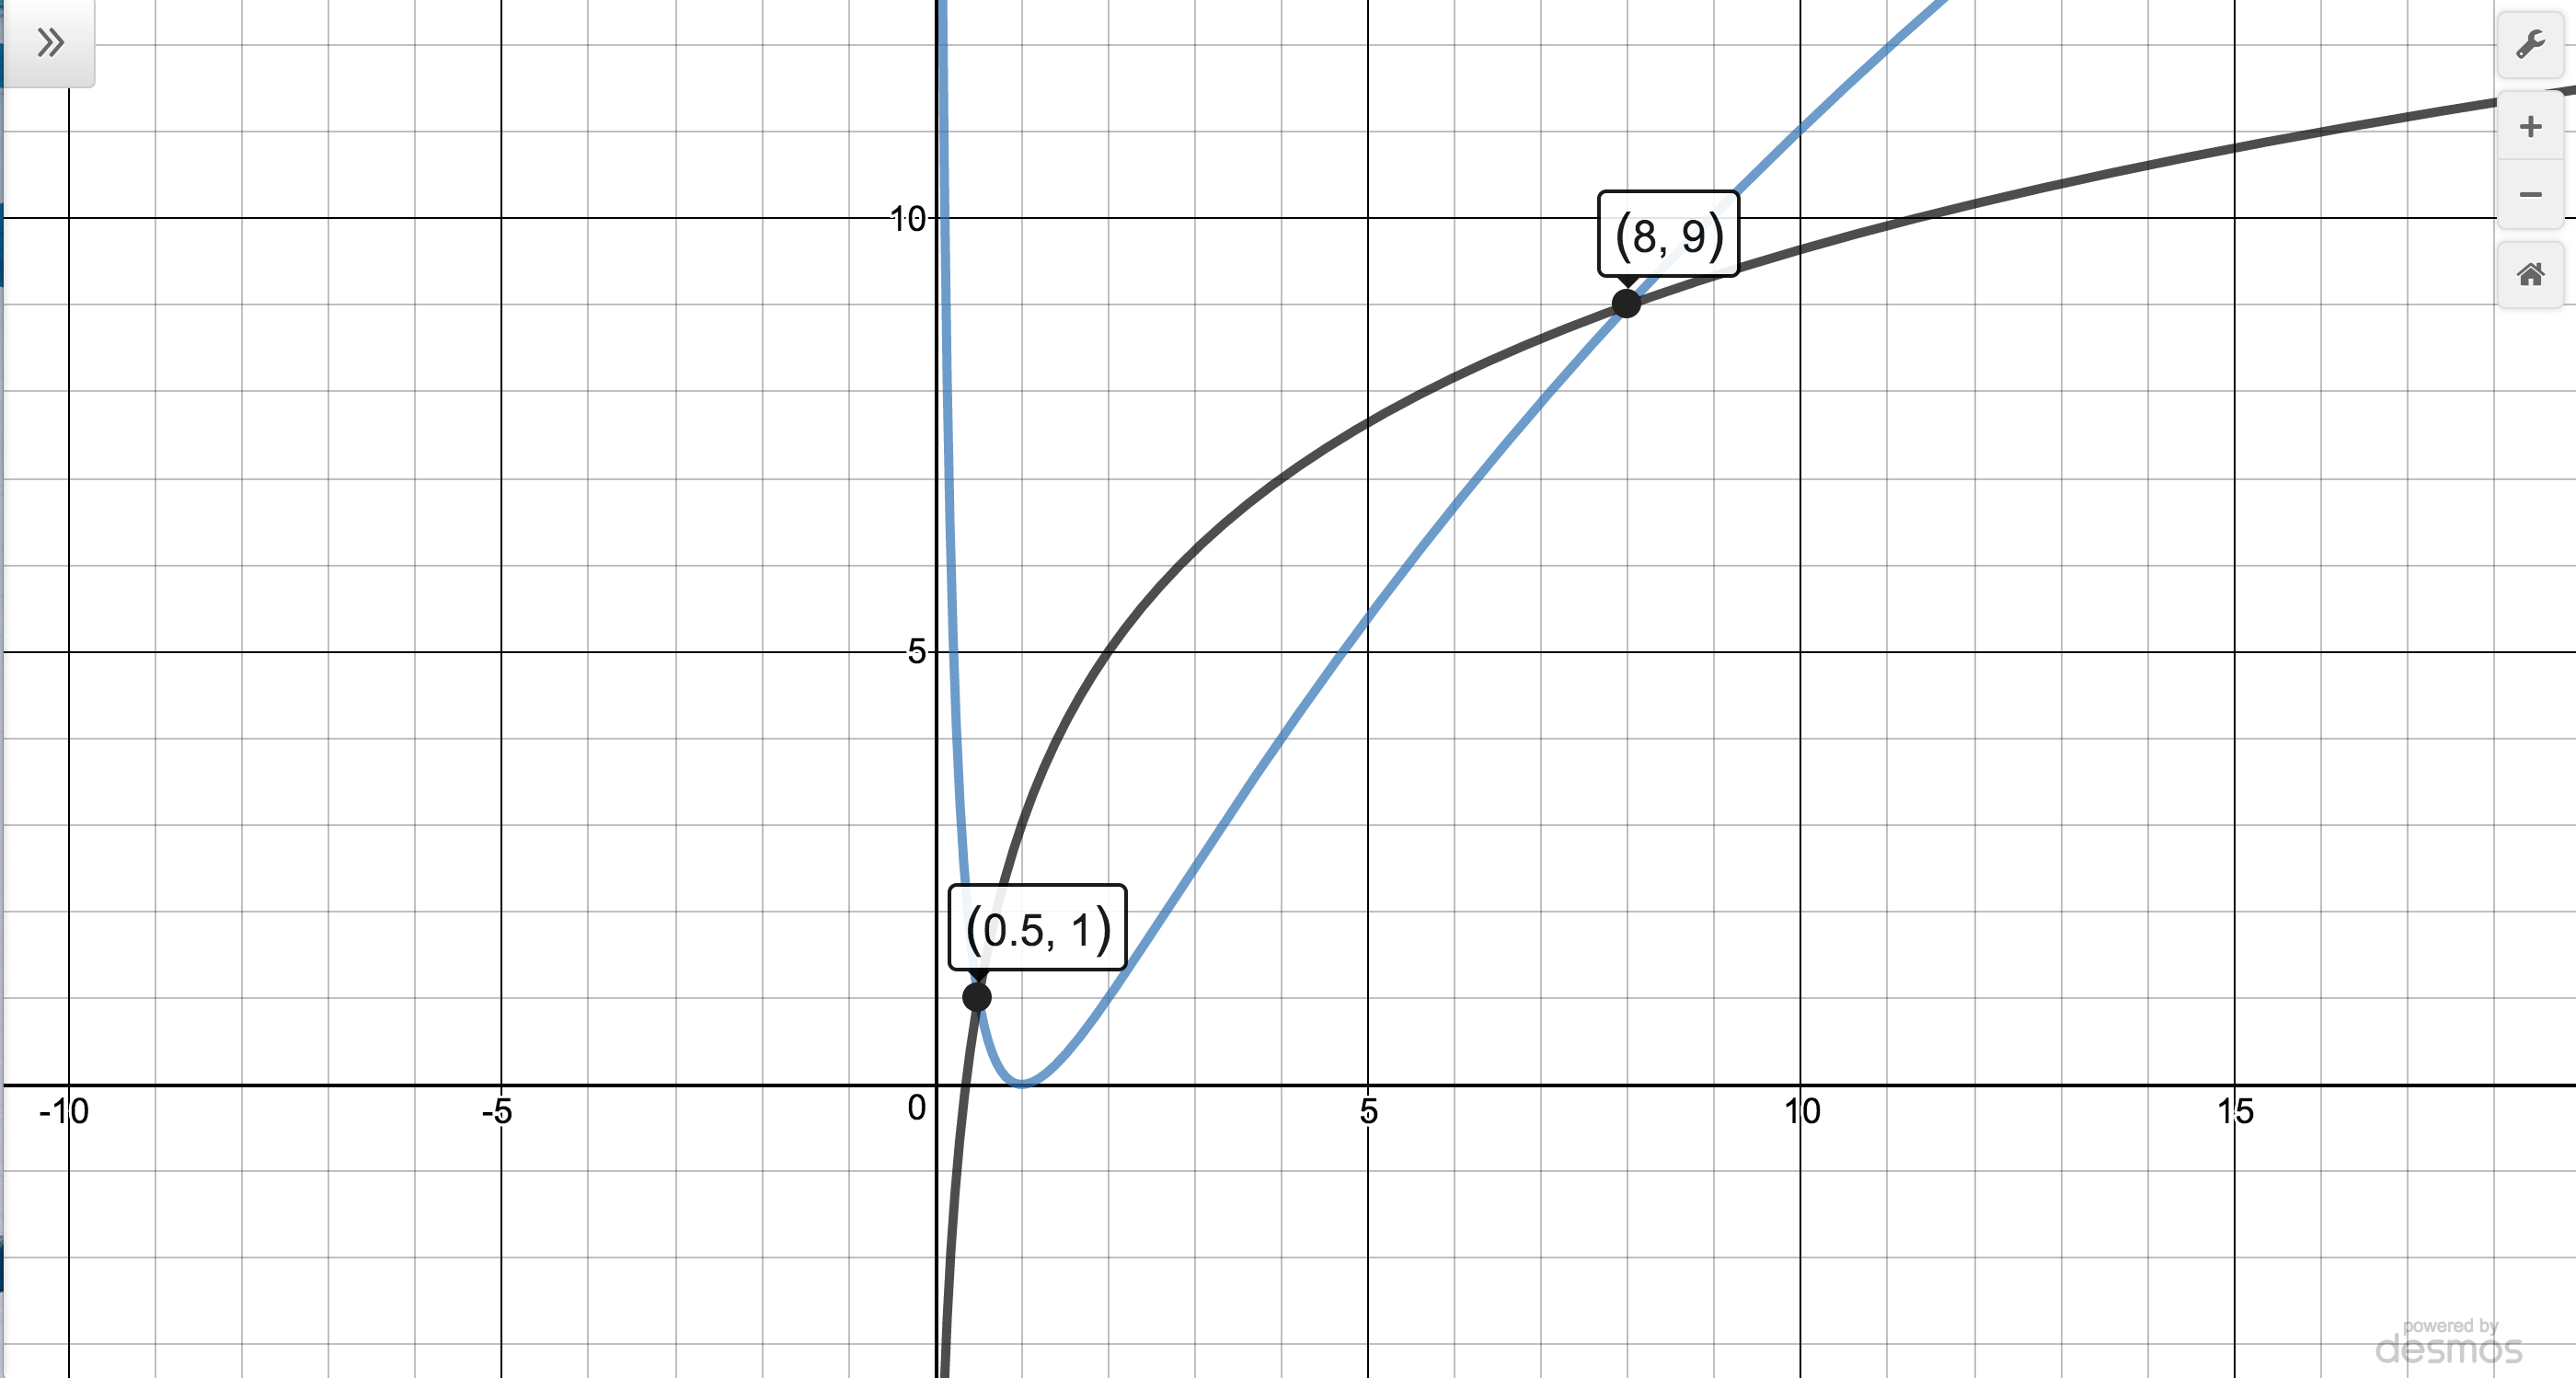
\includegraphics[width=3in]{./LogarithmicEquationsandInequalitiesGraphics/LogEqnEx08.jpg} \\

A sign diagram for 

&

Checking $\left(\log_{2}(x)\right)^2 < 2 \log_{2}(x) + 3$ \\

 $r(x) = \left(\log_{2}(x)\right)^2 - 2 \log_{2}(x) - 3$
 
 & \\

\end{tabular}

\end{center}



\item  We begin to solve $t \log(t+1) \geq t$ by subtracting $t$ from both sides to get $t \log(t+1)  - t \geq 0$.  

\smallskip

We define $r(t) = t \log(t+1)  - t $ and due to the presence of the logarithm, we require $t > -1$.  

\smallskip

To find the zeros of $r$, we set $r(t) = t \log(t+1)  - t = 0$.  Factoring, we get $t \left(\log(t+1) - 1\right) = 0$, which gives $t=0$ or $\log(t+1) - 1=0$.  

\smallskip

From $\log(t+1) - 1=0$ we get   $\log(t+1) = 1$, which we  rewrite as  $t+1 = 10^{1}$. Hence,   $t = 9$.  

\smallskip

We select test values $t$ so that $t+1$ is a power of $10$. Using $-1 < -0.9 < 0 < \sqrt{10} -1 < 9 < 99$,   our sign diagram gives the solution as $(-1,0] \cup [9, \infty)$. 

\smallskip

We find the graphs of  $y= f(t) = t \log(t+1)$  and $y=g(t) = t$ intersect at $t=0$ and $t=9$ with the graph of $f$ above the graph of $g$ on the given solution intervals.


\begin{center}

\begin{tabular}{m{2in}c}

\begin{mfpic}[10]{-6}{6}{-2}{2}
\arrow \polyline{(-6,0),(6,0)}
\xmarks{-2,2}
\scriptsize
\tlpointsep{4pt}
\normalsize
\tlabel[cc](-6,-1){$-1$}
\tlabel[cc](-4,1){$(+)$}
\tlabel[cc](-2,-1){$0$}
\tlabel[cc](-2,1){$0$}
\tlabel[cc](0,1){$(-)$}
\tlabel[cc](2,-1){$9$}
\tlabel[cc](2,1){$0$}
\tlabel[cc](4,1){$(+)$}
\pointfillfalse
\point[4pt]{(-6,0)}
\end{mfpic} 

& 


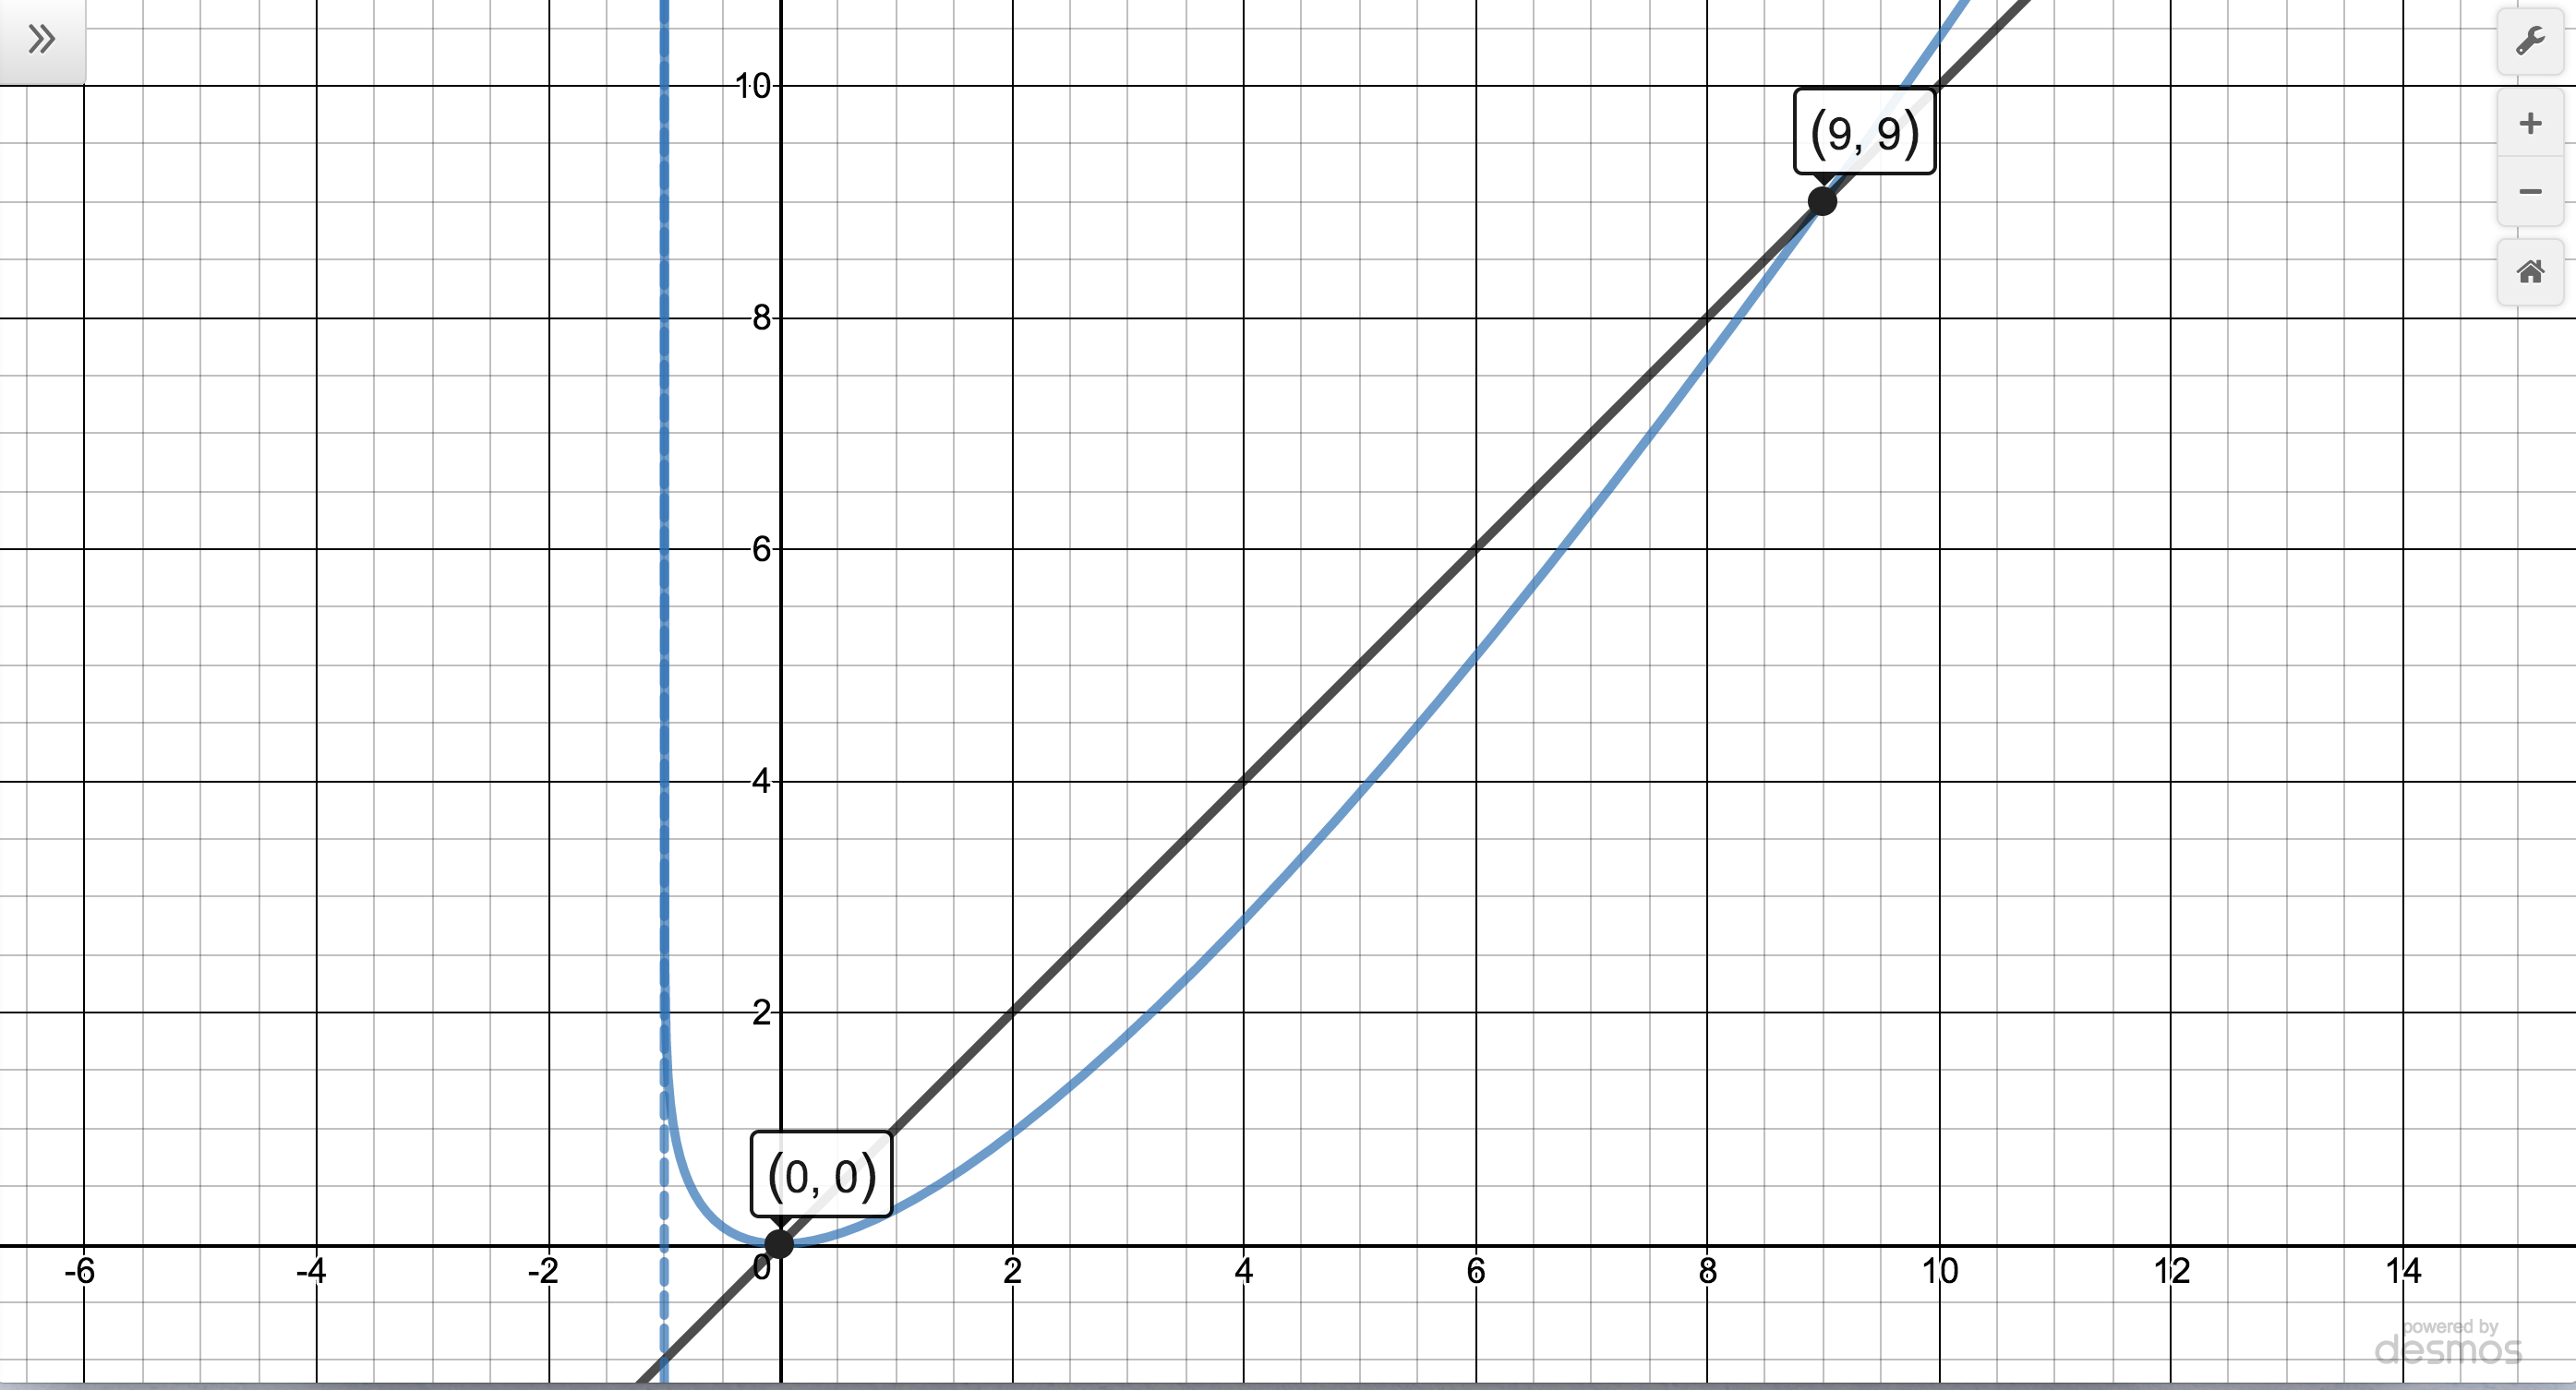
\includegraphics[width=3in]{./LogarithmicEquationsandInequalitiesGraphics/LogEqnEx09.jpg} \\

A sign diagram for   
&

Checking $t \log(t+1) \geq t$ \\

$r(t) = t \log(t+1)  - t $ & \\


\end{tabular}

\end{center}

\qed
\end{enumerate}
\end{ex}

\smallskip

Our next example revisits the concept of pH first seen in Exercise \ref{pHexercise} in Section \ref{LogarithmicFunctions}.  


\begin{ex}

In order to successfully breed Ippizuti fish the pH of a freshwater tank must be at least 7.8 but can be no more than 8.5.  Determine the corresponding range of hydrogen ion concentration, and check your answer using a calculator.

\smallskip

{\bf Solution.}  Recall from Exercise \ref{pHexercise} in Section \ref{LogarithmicFunctions} that $\text{pH} = -\log[\text{H}^{+}]$ where $[\text{H}^{+}]$ is the hydrogen ion concentration in moles per liter.  

\smallskip

We require $7.8 \leq -\log[\text{H}^{+}] \leq 8.5$ or $-8.5 \leq   \log[\text{H}^{+}] \leq -7.8$.  One way to proceed is to break this compound inequality into two inequalities, solve each using a sign diagram, and take the intersection of the solution sets.\footnote{Refer to page \pageref{intersectionunion} for a discussion of what this means.}  

\smallskip

On the other hand, we take advantage of the fact that $F(x) = 10^{x}$ is an increasing function, meaning that if $a \leq b \leq c$, then $10^{a} \leq 10^{b} \leq 10^{c}$.  This property allows us to solve our inequality in one step: from $-8.5 \leq   \log[\text{H}^{+}] \leq -7.8$, we get   $10^{-8.5} \leq   10^{\log[\text{H}^{+}]} \leq 10^{-7.8}$, so our solution is $ \leq   [\text{H}^{+}] \leq 10^{-7.8}$.  (Your Chemistry professor may want the answer written as $3.16 \times 10^{-9} \leq [\text{H}^{+}] \leq 1.58 \times 10^{-8}$.)  Using interval notation, our answer is $\left[10^{-8.5}, 10^{-7.8}\right]$.   

\smallskip

After \textit{very} carefully adjusting the viewing window on the graphing utility, we see the graph of $f(x) = -\log(x)$ lies between the lines $y = 7.8$ and $y = 8.5$ on the interval $[3.162 \times 10^{-9}, 1.5849 \times 10^{-8}]$.

\smallskip

\begin{center}

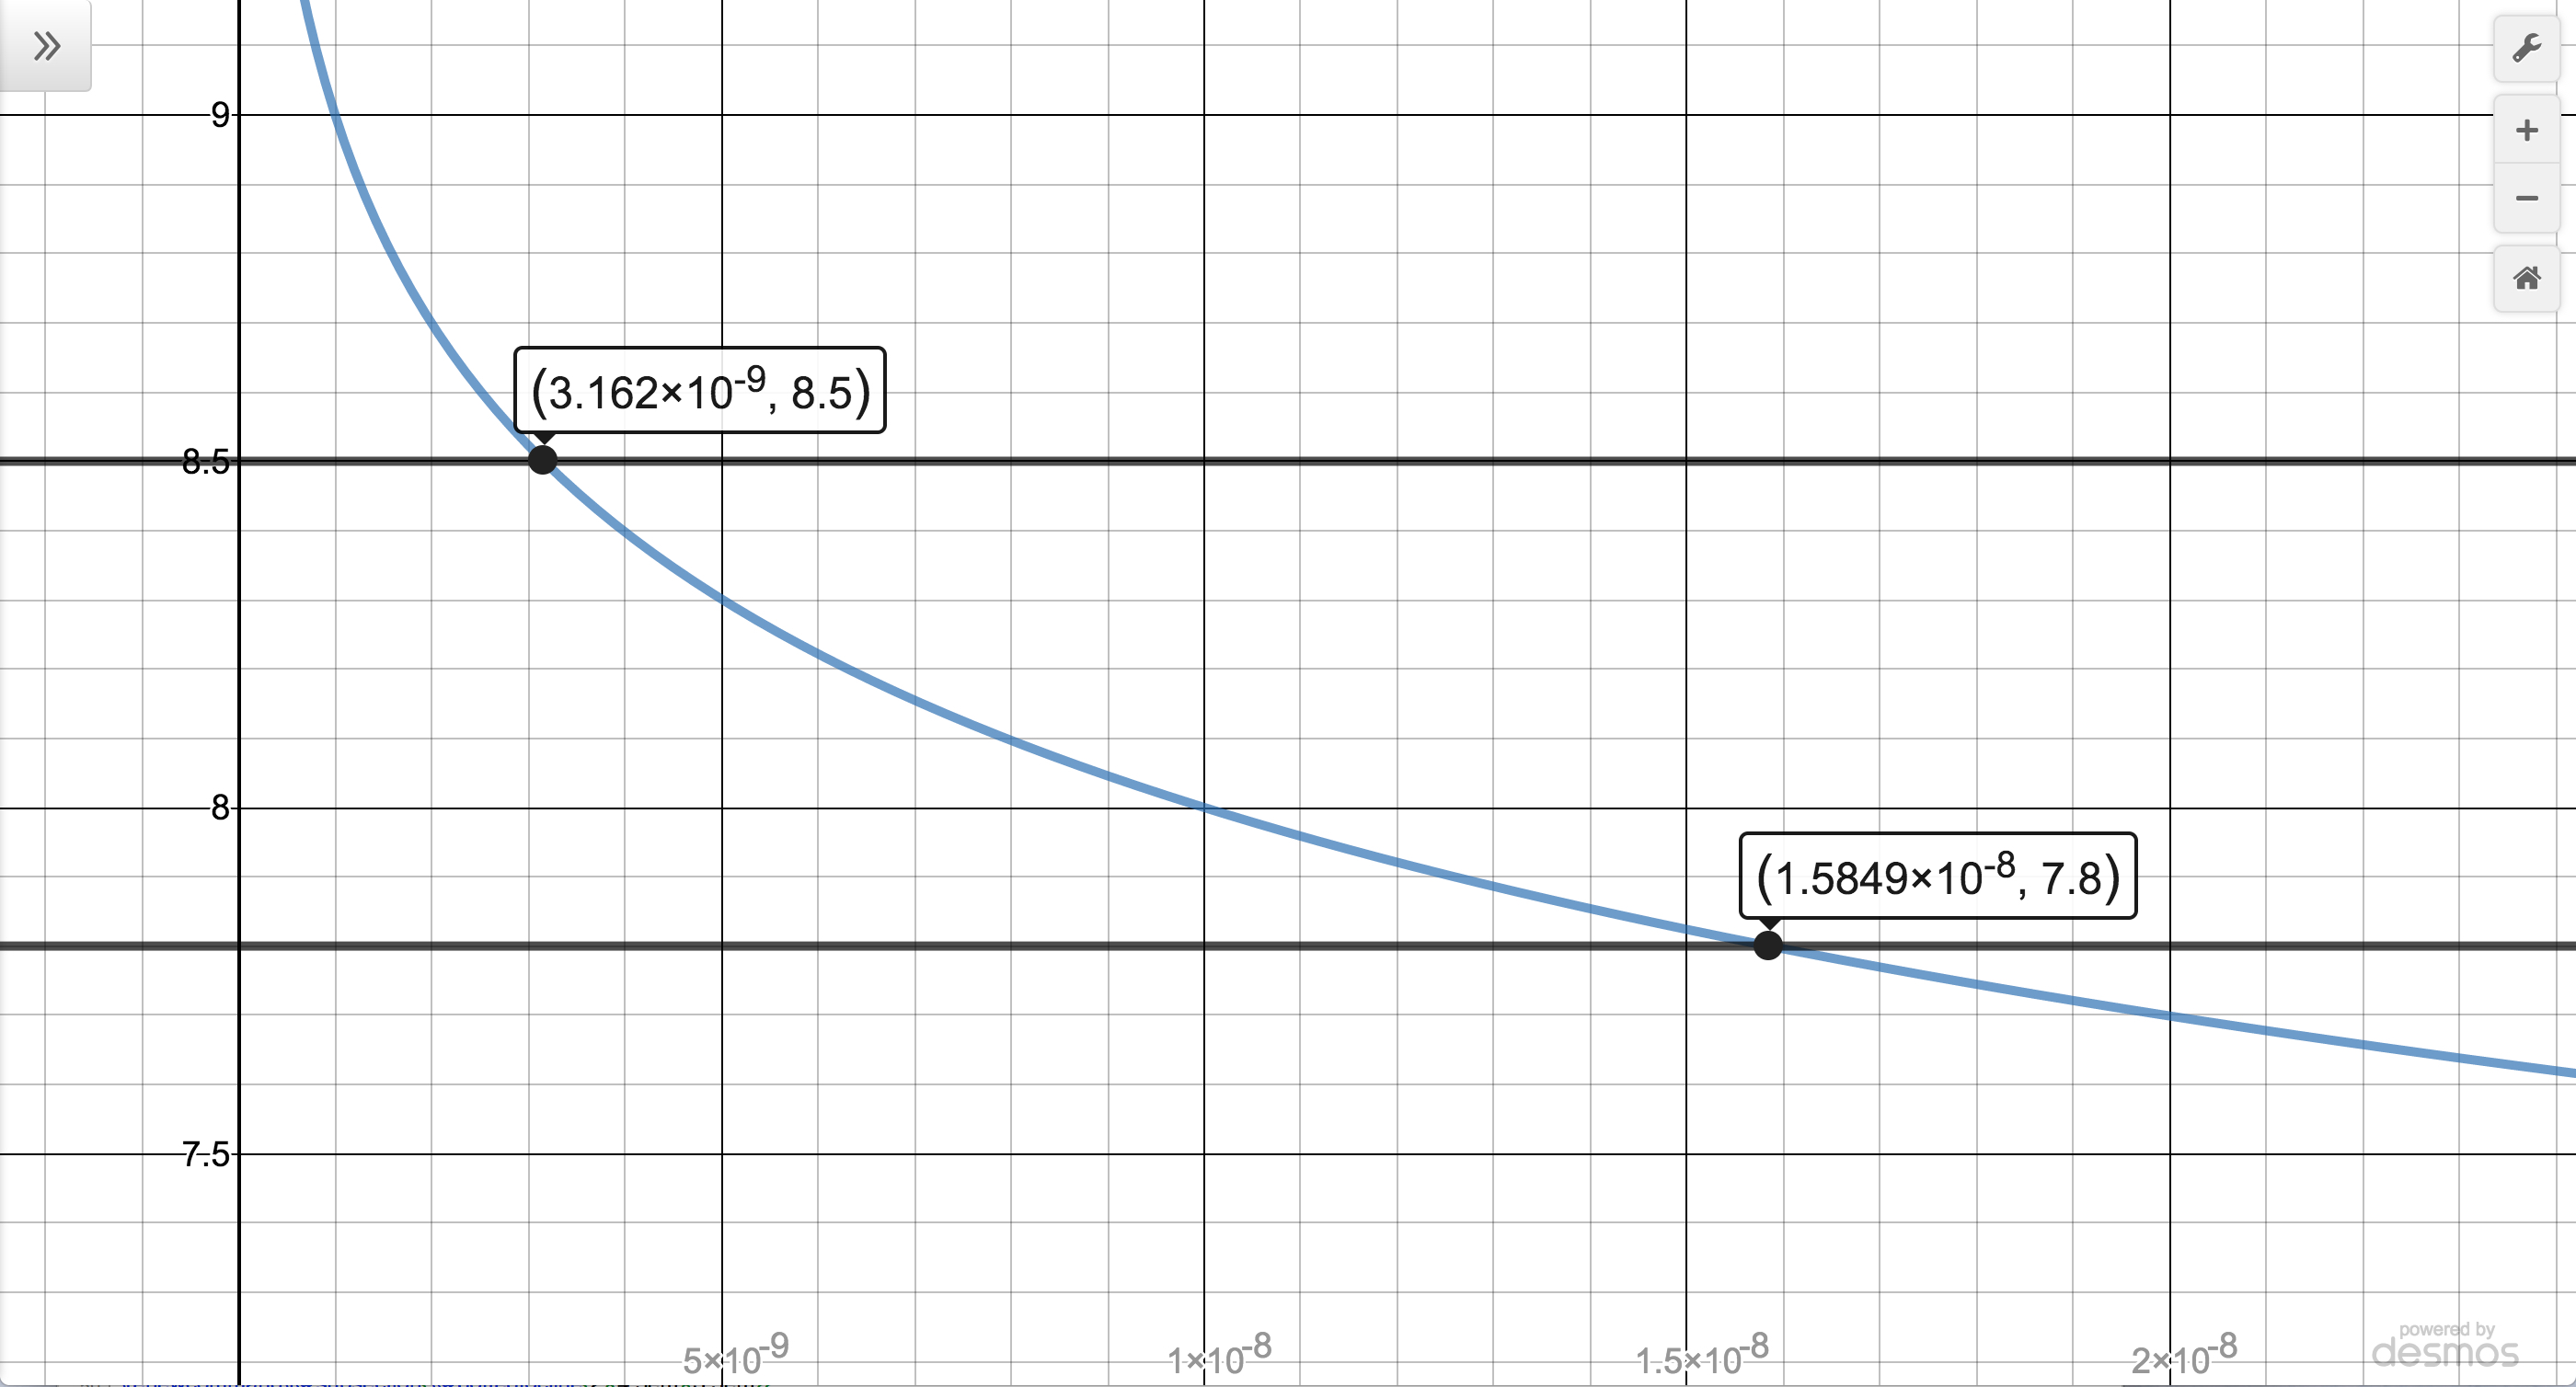
\includegraphics[width=4in]{./LogarithmicEquationsandInequalitiesGraphics/LogEqnEx10.jpg}

\end{center}

\qed

\end{ex}

\smallskip

We close this section by finding an inverse of a one-to-one function which involves logarithms.

\begin{ex}  \label{logfracinverse} The function $f(x) = \dfrac{\log(x)}{1-\log(x)}$ is one-to-one. 

\begin{enumerate}

\item  Find a formula for $f^{-1}(x)$ and check your answer graphically using a graphing utility.

\item Solve  $\dfrac{\log(x)}{1-\log(x)} = 1$

\end{enumerate}

{\bf Solution.} \begin{enumerate} \item  We first write $y=f(x)$ then interchange the $x$ and $y$ and solve for $y$.

\[ \begin{array}{rclr}
y & = & f(x) & \\ 
y  & = & \dfrac{\log(x)}{1-\log(x)} & \\[8pt]
x  & = & \dfrac{\log(y)}{1-\log(y)} & \text{Interchange $x$ and $y$.}\\[8pt]
x\left(1-\log(y)\right) & = & \log(y) & \\ 
x - x\log(y)  & = & \log(y) & \\ 
x & = & x \log(y) + \log(y) & \\ 
x & = & (x+1) \log(y) & \\ 
\dfrac{x}{x+1}  & = & \log(y) & \\ 
y & = & 10^{\frac{x}{x+1}} & \text{Rewrite as an exponential equation.}\\

\end{array}\]



We have $f^{-1}(x) = 10^{\frac{x}{x+1}}$.  Graphing $f$ and $f^{-1}$ on the same viewing window produces the required symmetry about $y=x$.

\begin{center}

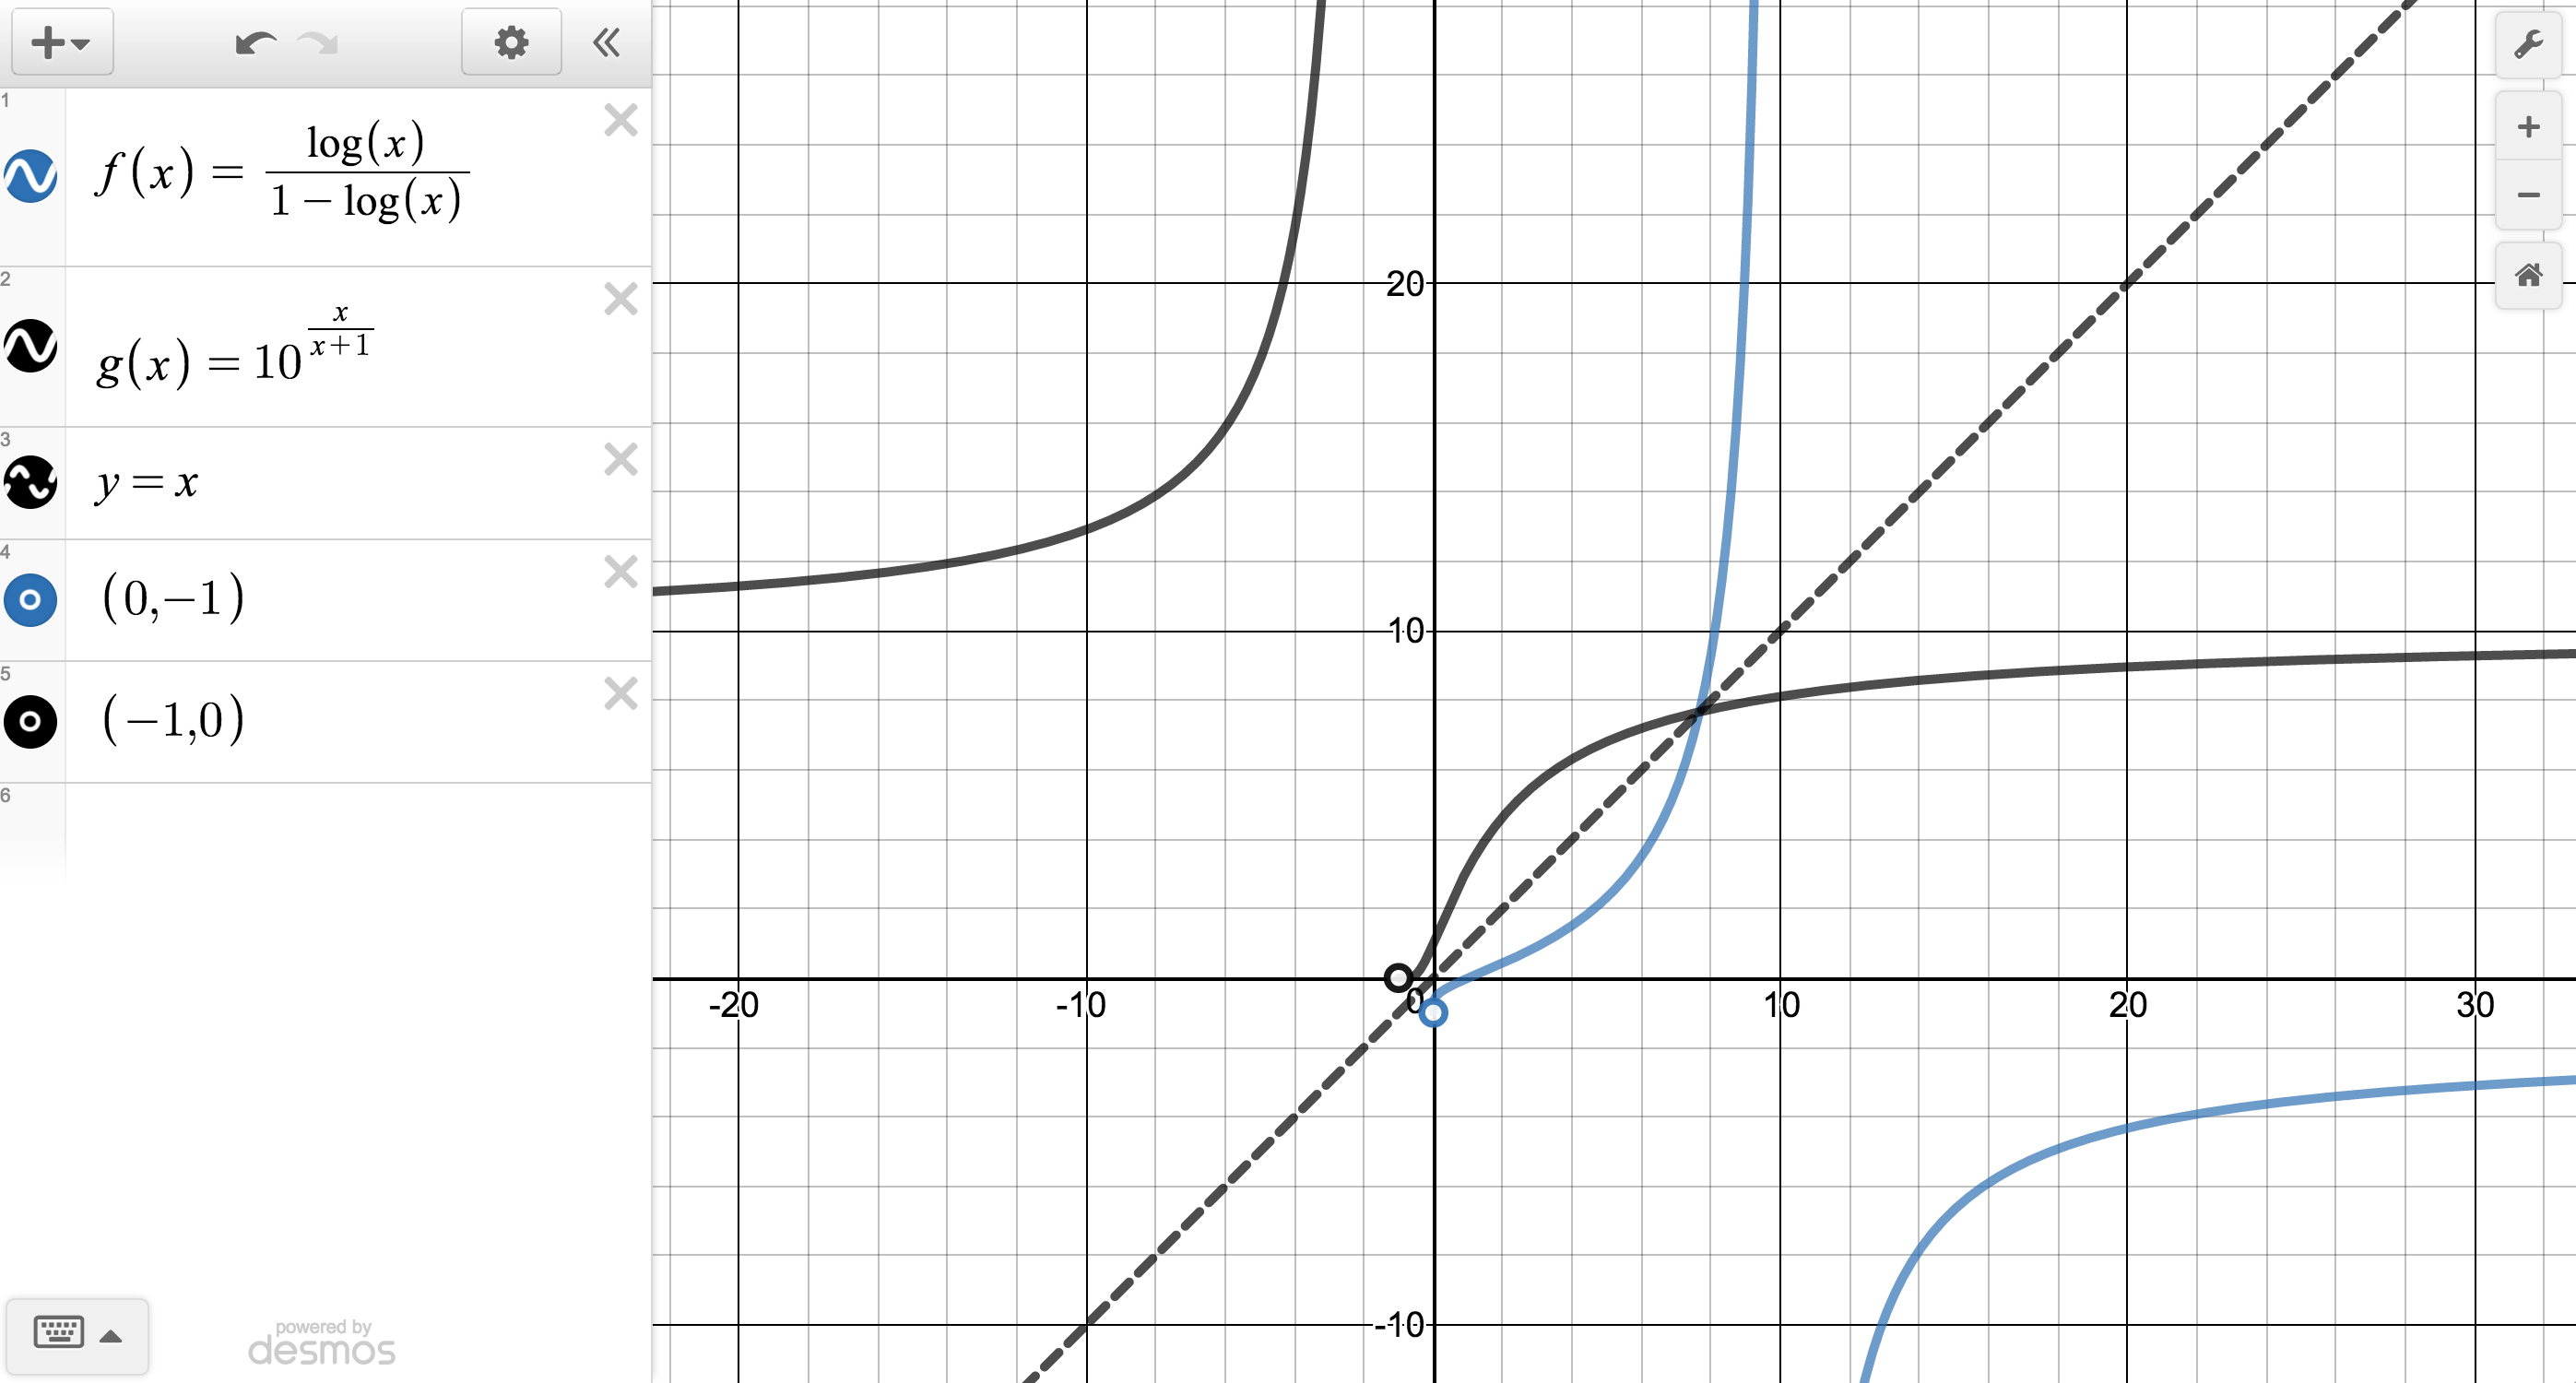
\includegraphics[width=4in]{./LogarithmicEquationsandInequalitiesGraphics/LogEqnEx11.jpg}

\end{center}

\item Recognizing   $\frac{\log(x)}{1-\log(x)} = 1$ as $f(x) = 1$, we have $x = f^{-1}(1) = 10^{\frac{1}{1+1}} = 10^{\frac{1}{2}} = \sqrt{10}$.

To check our answer algebraically,  first recall  $\log(\sqrt{10}) = \log_{10}(\sqrt{10})$.  Next, we know $\sqrt{10} = 10^{\frac{1}{2}}$.  Hence, $\log_{10} \left(10^{\frac{1}{2}} \right) = \frac{1}{2} = 0.5$.  It follows that $\frac{\log(\sqrt{10})}{1-\log(\sqrt{10})} = \frac{0.5}{1-0.5} = \frac{0.5}{0.5} = 1$, as required.  \qed

\end{enumerate}



\end{ex}
\end{comment}

\newpage

\subsection{Exercises}

\label{ExercisesforLogarithmicEquationsandInequalities}

In Exercises \ref{solvelogeqexfirst} - \ref{solvelogeqexlast}, solve the equation analytically.

\begin{multicols}{2}
\begin{enumerate}

\item $\log(3x-1) = \log(4-x)$  \phantom{$\log_{2}\left(x^{3}\right) = \log_{2}(x)$} \label{solvelogeqexfirst}

\item $\log_{2}\left(x^{3}\right) = \log_{2}(x)$

\setcounter{HW}{\value{enumi}}
\end{enumerate}
\end{multicols}

\begin{multicols}{2}
\begin{enumerate}
\setcounter{enumi}{\value{HW}}

\item $\ln\left(8-t^2\right)=\ln(2-t)$ \vphantom{$\log_{5}\left(18-t^2\right) = \log_{5}(6-t)$}

\item $\log_{5}\left(18-t^2\right) = \log_{5}(6-t)$

\setcounter{HW}{\value{enumi}}
\end{enumerate}
\end{multicols}

\begin{multicols}{2}
\begin{enumerate}
\setcounter{enumi}{\value{HW}}

\item $\log_{3}(7-2x) = 2$ \vphantom{$\log_{\frac{1}{2}} (2x-1) = -3$}
\item $\log_{\frac{1}{2}} (2x-1) = -3$

\setcounter{HW}{\value{enumi}}
\end{enumerate}
\end{multicols}

\begin{multicols}{2}
\begin{enumerate}
\setcounter{enumi}{\value{HW}}

\item $\ln\left(t^2-99\right) = 0$
\item $\log(t^2-3t) = 1$

\setcounter{HW}{\value{enumi}}
\end{enumerate}
\end{multicols}

\begin{multicols}{2}
\begin{enumerate}
\setcounter{enumi}{\value{HW}}

\item $\log_{125} \left(\dfrac{3x-2}{2x+3}\right)=\dfrac{1}{3}$

\item $\log\left(\dfrac{x}{10^{-3}}\right) = 4.7$ \vphantom{$\log_{125} \left(\dfrac{3x-2}{2x+3}\right)$} \label{sixfourRichterequ}


\setcounter{HW}{\value{enumi}}
\end{enumerate}
\end{multicols}


\begin{multicols}{2}
\begin{enumerate}
\setcounter{enumi}{\value{HW}}

\item $-\log(x) = 5.4$ \vphantom{$10\log\left(\dfrac{t}{10^{-12}}\right)$} \label{sixfourpHequ}
\item $10\log\left(\dfrac{x}{10^{-12}}\right) = 150$ \label{sixfourdecibelequ}

\setcounter{HW}{\value{enumi}}
\end{enumerate}
\end{multicols}

\begin{multicols}{2}
\begin{enumerate}
\setcounter{enumi}{\value{HW}}

\item $6-3\log_{5}(2t)=0$
\item $3\ln(t)-2=1-\ln(t)$

\setcounter{HW}{\value{enumi}}
\end{enumerate}
\end{multicols}

\begin{multicols}{2}
\begin{enumerate}
\setcounter{enumi}{\value{HW}}

\item $\log_{3}(t - 4) + \log_{3}(t + 4) = 2$

\item $\log_{5}(2t + 1) + \log_{5}(t + 2) = 1$

\setcounter{HW}{\value{enumi}}
\end{enumerate}
\end{multicols}

\begin{multicols}{2}
\begin{enumerate}
\setcounter{enumi}{\value{HW}}

\item $\log_{169}(3x + 7) - \log_{169}(5x - 9) = \dfrac{1}{2}$

\item $\ln(x+1) - \ln(x) = 3$ \vphantom{$\log_{169}(3x + 7)$}

\setcounter{HW}{\value{enumi}}
\end{enumerate}
\end{multicols}

\begin{multicols}{2}
\begin{enumerate}
\setcounter{enumi}{\value{HW}}

\item $2\log_{7}(t) = \log_{7}(2) + \log_{7}(t+12)$

\item $\log(t) - \log(2) = \log(t+8)  - \log(t+2)$

\setcounter{HW}{\value{enumi}}
\end{enumerate}
\end{multicols}

\begin{multicols}{2}
\begin{enumerate}
\setcounter{enumi}{\value{HW}}

\item $\log_{3}(x) = \log_{\frac{1}{3}}(x) + 8$

\item $\ln(\ln(x)) = 3$

\setcounter{HW}{\value{enumi}}
\end{enumerate}
\end{multicols}

\begin{multicols}{2}
\begin{enumerate}
\setcounter{enumi}{\value{HW}}

\item $\left(\log(t)\right)^2=2\log(t)+15$

\item $\ln(t^{2}) = (\ln(t))^{2}$ \label{solvelogeqexlast}

\setcounter{HW}{\value{enumi}}
\end{enumerate}
\end{multicols}


In Exercises \ref{solvelogineqexfirst} - \ref{solvelogineqexlast}, solve the inequality analytically.

\begin{multicols}{2}
\begin{enumerate}
\setcounter{enumi}{\value{HW}}

\item $\dfrac{1 - \ln(t)}{t^{2}} < 0$ \label{solvelogineqexfirst}
\item $t\ln(t) - t > 0$ \phantom{$\dfrac{1 - \ln(x)}{x^{2}} < 0$}  


\setcounter{HW}{\value{enumi}}
\end{enumerate}
\end{multicols}

\begin{multicols}{2}
\begin{enumerate}
\setcounter{enumi}{\value{HW}}

\item $10\log\left(\dfrac{x}{10^{-12}}\right) \geq 90$ \label{sixfourdecibelineq} 
\item $5.6 \leq \log\left(\dfrac{x}{10^{-3}}\right) \leq 7.1$ \label{sixfourRichterineq}


\setcounter{HW}{\value{enumi}}
\end{enumerate}
\end{multicols}

\begin{multicols}{2}
\begin{enumerate}
\setcounter{enumi}{\value{HW}}


\item $2.3 < -\log(x) < 5.4$ \label{sixfourpHineq} 

\item $\ln(t^{2}) \leq (\ln(t))^{2}$ \label{solvelogineqexlast} 

\setcounter{HW}{\value{enumi}}
\end{enumerate}
\end{multicols}

\pagebreak

In Exercises \ref{logeqcalcexfirst} - \ref{logeqcalcexlast}, use a graphing utility to help you solve the equation or  inequality.

\begin{multicols}{2}
\begin{enumerate}
\setcounter{enumi}{\value{HW}}

\item $\ln(t) = e^{-t}$ \label{logeqcalcexfirst} 
\item $\ln(x) = \sqrt[4]{x}$ 

\setcounter{HW}{\value{enumi}}
\end{enumerate}
\end{multicols}

\begin{multicols}{2}
\begin{enumerate}
\setcounter{enumi}{\value{HW}}

\item $\ln(t^{2} + 1) \geq 5$
\item $\ln(-2x^{3} - x^{2} + 13x - 6) < 0$ \label{logeqcalcexlast} 

\setcounter{HW}{\value{enumi}}
\end{enumerate}
\end{multicols}


In Exercises \ref{domaincomplicatedlogfirst} - \ref{domaincomplicatedloglast},  find the domain of the function.

\begin{multicols}{2} 
\begin{enumerate}
\setcounter{enumi}{\value{HW}}

\item \label{domaincomplicatedlogfirst}  $r(x) =   \dfrac{x}{1 - \ln(x)}$  %(-\infty, e) \cup (e, \infty)$

\item   $R(x) = \dfrac{x \ln(x)}{1 - \ln(x)}$   % $(0,e) \cup (e, \infty)$

\setcounter{HW}{\value{enumi}}
\end{enumerate}
\end{multicols}


\begin{multicols}{2} 
\begin{enumerate}
\setcounter{enumi}{\value{HW}}

\item     $s(t) = \sqrt{2 - \log(t)}$  \vphantom{$c(t) =  (2 \ln(t) -1)^{\frac{2}{3}}$} %$(0, 100]$
\item     $c(t) =  (2 \ln(t) -1)^{\frac{2}{3}}$  %$(0, \infty)$

\setcounter{HW}{\value{enumi}}
\end{enumerate}
\end{multicols}

\begin{multicols}{2} 
\begin{enumerate}
\setcounter{enumi}{\value{HW}}
  
\item     $\ell(t) = \ln( \ln(t))$  \vphantom{$L(x) = \log\left( \dfrac{x \ln(x)}{1 - \ln(x)} \right)$} %$(1, \infty)$    

\item  \label{domaincomplicatedloglast}    $L(x) = \log\left( \dfrac{x \ln(x)}{1 - \ln(x)} \right)$  %$(1,e)$ 


\setcounter{HW}{\value{enumi}}
\end{enumerate}
\end{multicols}


\begin{enumerate}
\setcounter{enumi}{\value{HW}}

\item \label{onetooneexpexercise} Since $f(x) = e^{x}$ is a strictly increasing function, if $a < b$ then $e^{a} < e^{b}$.  Use this fact to solve the inequality $\ln(2x + 1) < 3$ without a sign diagram. Use this technique to solve the inequalities in Exercises \ref{sixfourdecibelineq} - \ref{sixfourpHineq}. (Compare this to Exercise  \ref{onetoonelogexercise} in Section \ref{ExponentialEquationsandInequalities}.)

\item Solve $\ln(3 - y) - \ln(y) = 2x + \ln(5)$ for $y$.

\item \co{In Example \ref{logfracinverse} we found t}The inverse of $f(x) = \dfrac{\log(x)}{1-\log(x)}$ to be $f^{-1}(x) = 10^{\frac{x}{x+1}}$.

\begin{enumerate}

\item Algebraically check our answer by verifying  $\left(f^{-1} \circ f\right)(x) = x$ for all $x$ in the domain of $f$ and that $\left(f \circ f^{-1}\right)(x) = x$ for all $x$ in the domain of $f^{-1}$.

\item Find the range of $f$ by finding the domain of $f^{-1}$.

\item Let $g(x) = \dfrac{x}{1 - x}$ and $h(x) = \log(x)$.  Show that $f = g \circ h$ and $(g \circ h)^{-1} = h^{-1} \circ g^{-1}$.\\


NOTE:  We know this is true in general by Exercise \ref{fcircginverse} in Section \ref{InverseFunctions}, but it's nice to see a specific example of the property.

\end{enumerate}

\item \label{inversehyptangent} Let $f(x) = \dfrac{1}{2}\ln\left(\dfrac{1 + x}{1 - x}\right)$.  Compute $f^{-1}(x)$ and find its domain and range.

\item Explain the equation in Exercise \ref{sixfourRichterequ} and the inequality in Exercise \ref{sixfourRichterineq} above in terms of the Richter scale for earthquake magnitude.  (See Exercise \ref{Richterexercise} in Section \ref{ExponentialFunctions}.)

\item Explain the equation in Exercise \ref{sixfourdecibelequ} and the inequality in Exercise \ref{sixfourdecibelineq} above in terms of sound intensity level as measured in decibels.  (See Exercise \ref{decibelexercise} in Section \ref{ExponentialFunctions}.)

\item Explain the equation in Exercise \ref{sixfourpHequ} and the inequality in Exercise \ref{sixfourpHineq} above in terms of the pH of a solution.  (See Exercise \ref{pHexercise} in Section \ref{ExponentialFunctions}.)

\item With the help of your classmates, solve the inequality $\sqrt[n]{x} > \ln(x)$ for a variety of natural numbers $n$.  What might you conjecture about the ``speed'' at which $f(x) = \ln(x)$ grows versus any principal $n^{\textrm{th}}$ root function?

\end{enumerate}

\newpage

\subsection{Answers}
\begin{multicols}{3}
\begin{enumerate}

\item $x = \frac{5}{4}$
\item $x = 1$
\item $t=-2$

\setcounter{HW}{\value{enumi}}
\end{enumerate}
\end{multicols}

\begin{multicols}{3}
\begin{enumerate}
\setcounter{enumi}{\value{HW}}

\item $t=-3,\, 4$
\item $x=-1$
\item $x=\frac{9}{2}$

\setcounter{HW}{\value{enumi}}
\end{enumerate}
\end{multicols}

\begin{multicols}{3}
\begin{enumerate}
\setcounter{enumi}{\value{HW}}

\item $t=\pm 10$
\item $t=-2,\, 5$
\item $x = -\frac{17}{7}$

\setcounter{HW}{\value{enumi}}
\end{enumerate}
\end{multicols}

\begin{multicols}{3}
\begin{enumerate}
\setcounter{enumi}{\value{HW}}

\item $x = 10^{1.7}$
\item $x = 10^{-5.4}$
\item $x = 10^{3}$

\setcounter{HW}{\value{enumi}}
\end{enumerate}
\end{multicols}

\begin{multicols}{3}
\begin{enumerate}
\setcounter{enumi}{\value{HW}}

\item $t=\frac{25}{2}$
\item $t=e^{3/4}$
\item $t = 5$

\setcounter{HW}{\value{enumi}}
\end{enumerate}
\end{multicols}

\begin{multicols}{3}
\begin{enumerate}
\setcounter{enumi}{\value{HW}}

\item $t = \frac{1}{2}$
\item $x = 2$
\item $x = \frac{1}{e^3-1}$

\setcounter{HW}{\value{enumi}}
\end{enumerate}
\end{multicols}

\begin{multicols}{3}
\begin{enumerate}
\setcounter{enumi}{\value{HW}}

\item $t=6$
\item $t=4$
\item $x = 81$

\setcounter{HW}{\value{enumi}}
\end{enumerate}
\end{multicols}

\begin{multicols}{3}
\begin{enumerate}
\setcounter{enumi}{\value{HW}}

\item $x = e^{e^3}$
\item $t=10^{-3}, \, 10^{5}$
\item $t = 1, \, x = e^{2}$

\setcounter{HW}{\value{enumi}}
\end{enumerate}
\end{multicols}

\begin{multicols}{3}
\begin{enumerate}
\setcounter{enumi}{\value{HW}}

\item $(e, \infty)$
\item $(e, \infty)$
\item $\left[10^{-3}, \infty \right)$

\setcounter{HW}{\value{enumi}}
\end{enumerate}
\end{multicols}

\begin{multicols}{3}
\begin{enumerate}
\setcounter{enumi}{\value{HW}}

\item $\left[10^{2.6}, 10^{4.1}\right]$

\item $\left(10^{-5.4}, 10^{-2.3}\right)$
\item $(0, 1] \cup [e^{2}, \infty)$

\setcounter{HW}{\value{enumi}}
\end{enumerate}
\end{multicols}

\begin{multicols}{2}
\begin{enumerate}
\setcounter{enumi}{\value{HW}}

\item $t \approx 1.3098$
\item $x \approx 4.177, \, x \approx 5503.665$

\setcounter{HW}{\value{enumi}}
\end{enumerate}
\end{multicols}

\begin{multicols}{2}
\begin{enumerate}
\setcounter{enumi}{\value{HW}}

\item $\approx (-\infty, -12.1414) \cup (12.1414, \infty)$
\item $\approx (-3.0281, -3) \cup (0.5, 0.5991) \cup (1.9299, 2)$

\setcounter{HW}{\value{enumi}}
\end{enumerate}
\end{multicols}

\begin{multicols}{3} 
\begin{enumerate}
\setcounter{enumi}{\value{HW}}

\item  $(-\infty, e) \cup (e, \infty)$

\item   $(0,e) \cup (e, \infty)$

\item  $(0, 100]$

\setcounter{HW}{\value{enumi}}
\end{enumerate}
\end{multicols}


\begin{multicols}{3} 
\begin{enumerate}
\setcounter{enumi}{\value{HW}}

\item    $(0, \infty)$
  
\item    $(1, \infty)$    

\item    $(1,e)$ 


\setcounter{HW}{\value{enumi}}
\end{enumerate}
\end{multicols}


\begin{multicols}{2}
\begin{enumerate}
\setcounter{enumi}{\value{HW}}

\item $-\dfrac{1}{2} < x < \dfrac{e^{3} - 1}{2}$, so $\left( -\dfrac{1}{2}, \dfrac{e^{3} - 1}{2}\right)$

\item $y = \dfrac{3}{5e^{2x} + 1}$ \vphantom{$\dfrac{e^{3} - 1}{2}$}

\setcounter{HW}{\value{enumi}}
\end{enumerate}
\end{multicols}

\begin{enumerate}
\setcounter{enumi}{\value{HW}}
\addtocounter{enumi}{1}

\item $f^{-1}(x) = \dfrac{e^{2x} - 1}{e^{2x} + 1} = \dfrac{e^{x} - e^{-x}}{e^{x} + e^{-x}}$. 

\co{To see why we rewrite this in this form, see  Exercise \ref{andtheresthyperbolic} in Section \ref{ParametricEquations}.}

 The domain of $f^{-1}$ is $(-\infty, \infty)$ and its range is the same as the domain of $f$, namely $(-1, 1)$.

\end{enumerate}



\closegraphsfile


\begin{comment}
\newpage

\section{Applications of Exponential and Logarithmic Functions}

\opengraphsfile{ApplicationsofExponentialandLogarithmicFunctions}

\setcounter{footnote}{0}

\label{ExpLogApplications}

As we mentioned in Sections \ref{ExponentialFunctions} and \ref{LogarithmicFunctions}, exponential and logarithmic functions are used to model a wide variety of behaviors in the real world.  In the examples that follow, note that while the applications are drawn from many different disciplines, the mathematics remains essentially the same.  Due to the applied nature of the problems we will examine in this section, we will often express our final answers as decimal approximations (after finding exact answers first, of course!)

\subsection{Applications of Exponential Functions}
\label{expapp}

Perhaps the most well-known application of exponential functions comes from the financial world.  Suppose you have $ \$ 100$ to invest at your local bank and they are offering a whopping $5 \, \%$ annual percentage interest rate.  This means that after one year, the bank will pay \textit{you} $5 \%$ of that $\$100$, or $ \$ 100(0.05) =\$ 5$ in interest, so you now have $\$105$. This is in accordance with the formula for  \textit{simple interest} which you have undoubtedly run across at some point before.

\smallskip

\colorbox{ResultColor}{\bbm

\begin{eqn} \index{interest ! simple} \index{simple interest} \label{simpleinterest} \textbf{Simple Interest:} 

The amount of interest $I$ accrued at an annual rate $r$ on an investment\footnote{Called the \index{principal} \textbf{principal}} $P$ after $t$ years is  \[I = Prt\]  The amount  in the account after $t$ years, $A(t)$ is given by \[A(t) = P + I = P + Prt = P(1+rt)\]

\end{eqn}

\ebm}
\smallskip

Suppose, however, that six months into the year, you hear of a better deal at a rival bank.\footnote{Some restrictions may apply.} Naturally, you withdraw your money and try to invest it at the higher rate there.  Since six months is one half of a year, that initial $\$100$ yields $\$100(0.05)\left(\frac{1}{2}\right) = \$ 2.50$ in interest.  

\smallskip

You take your $\$102.50$ off to the competitor and find out that those restrictions which \textit{may} apply actually \underline{do} apply, so you return to your bank and re-deposit the $\$102.50$ for the remaining six months of the year. 

\smallskip 

To your surprise and delight, at the end of the year your statement reads $\$105.06$, not $\$105$ as you had expected.\footnote{Actually, the final balance should be $\$105.0625$.}  Where did those extra six cents come from?  

\smallskip

For the first six months of the year, interest was earned on the original principal of $\$100$, but for the second six months, interest was earned on $\$102.50$, that is, you earned interest on your interest.  This is the basic concept behind \textbf{compound interest}. 

\smallskip

In the previous discussion, we would say that the interest was compounded twice per year, or semiannually.\footnote{Using this convention, simple interest after one year is the same as compounding the interest only once.}  If more money can be earned by earning interest on interest already earned, one wonders what happens if the interest is compounded more often, say every three months -  $4$ times a year, or `quarterly.' 

\smallskip

In this case, the money is in the account for three months, or $\frac{1}{4}$ of a year, at a time.  After the first quarter, we have $A = P(1+rt) =  \$100 \left(1 + 0.05 \cdot \frac{1}{4} \right) = \$101.25$.  We now invest the $\$101.25$ for the next three months and find that at the end of the second quarter, we have $A =  \$101.25 \left(1 + 0.05 \cdot \frac{1}{4} \right)\approx \$102.51$.  Continuing in this manner, the balance at the end of the third quarter is $\$103.79$, and, at last, we obtain $\$105.08$.  The extra two cents hardly seems worth it, but we see that we do in fact get more money the more often we compound. 

\smallskip

In order to develop a formula for this phenomenon, we need to do some abstract calculations.  Suppose we wish to invest our principal $P$ at an annual rate $r$ and compound the interest $n$ times per year.  This means the money sits in the account $\frac{1}{n}^{\mbox{\tiny th}}$ of a year between compoundings.  Let $A_{k}$ denote the amount in the account after the $k^{\mbox{\tiny th}}$ compounding. 

\smallskip

Then $A_{\mbox{\tiny$1$}} = P\left(1 + r\left(\frac{1}{n}\right)\right)$ which simplifies to $A_{\mbox{\tiny$1$}} = P \left(1 + \frac{r}{n}\right)$.  After the second compounding, we use $A_{\mbox{\tiny$1$}}$ as our new principal and get $A_{\mbox{\tiny$2$}} = A_{\mbox{\tiny$1$}} \left(1 + \frac{r}{n}\right) = \left[P \left(1 + \frac{r}{n}\right)\right]\left(1 + \frac{r}{n}\right) = P \left(1 + \frac{r}{n}\right)^2$.  Continuing in this fashion, we get $A_{\mbox{\tiny$3$}} =P \left(1 + \frac{r}{n}\right)^3$, $A_{\mbox{\tiny$4$}} =P \left(1 + \frac{r}{n}\right)^4$, and so on, so that $A_{k} = P \left(1 + \frac{r}{n}\right)^k$.  

\smallskip

Since we compound the interest $n$ times per year, after $t$ years, we have $nt$ compoundings. We have just derived the general formula for compound interest below.

\smallskip

\colorbox{ResultColor}{\bbm

\begin{eqn} \index{interest ! compound} \index{compound interest} \label{compoundinterest} \textbf{Compounded Interest:}  

If an initial principal $P$ is invested at an annual rate $r$ and the interest is compounded $n$ times per year, the amount in the account after $t$ years, $A(t)$  is given by \[A(t) = P \left(1 + \frac{r}{n}\right)^{nt}\]

\end{eqn}

\ebm}

\smallskip

If we take $P = 100$, $r = 0.05$, and $n = 4$, Equation \ref{compoundinterest} becomes $A(t) = 100\left(1+ \frac{0.05}{4}\right)^{4t}$ which reduces to $A(t) = 100(1.0125)^{4t}$.  To check this new formula against our previous calculations, we find $A\left(\frac{1}{4}\right) = 100(1.0125)^{4 \left(\frac{1}{4}\right)} = 101.25$, $A\left(\frac{1}{2}\right) \approx \$102.51$, $A\left(\frac{3}{4}\right) \approx \$103.79$, and $A(1) \approx \$105.08$.

\begin{ex}  \label{compoundinterestex} Suppose $\$2000$ is invested in an account which offers $7.125 \%$ compounded monthly.

\begin{enumerate}

\item Express the amount $A(t)$ in the account as a function of the term of the investment $t$ in years.

\item  How much is in the account after $5$ years? 

\item  How long will it take for the initial investment to double?

\item  Find and interpret the average rate of change\footnote{See Definition \ref{arc} in Section \ref{ConstantandLinearFunctions}.} of the amount in the account:

\begin{itemize}

\item  from the end of the fourth year to the end of the fifth year

\item from the end of the thirty-fourth year to the end of the thirty-fifth year.

\end{itemize}

\pagebreak

\item  Find and interpret the relative rate of change\footnote{See Definition \ref{rrc} in Section \ref{ExponentialFunctions}.} of the amount in the account: 

\begin{itemize}

\item  from the end of the fourth year to the end of the fifth year

\item from the end of the thirty-fourth year to the end of the thirty-fifth year.

\end{itemize}

\end{enumerate}

{\bf Solution.}  

\begin{enumerate}

\item  Substituting $P = 2000$, $r = 0.07125$, and $n = 12$ (since interest is compounded \textit{monthly}) into Equation \ref{compoundinterest} yields $A(t) = 2000\left(1 + \frac{0.07125}{12}\right)^{12t}=2000 (1.0059375)^{12t}$.

\item  To find the amount in the account after $5$ years, we compute $A(5) = 2000 (1.0059375)^{12(5)} \approx 2852.92$.  After $5$ years, we have approximately $\$2852.92$.

\item  Our initial investment is $\$2000$, so to find the time it takes this to double, we need to find $t$ when $A(t) = 4000$.  That is, we need to solve $2000 (1.0059375)^{12t}=4000$, or $(1.0059375)^{12t}=2$.  

\smallskip

Taking natural logs as in Section \ref{ExponentialEquationsandInequalities}, we get $t = \frac{\ln(2)}{12 \ln(1.0059375)} \approx 9.75$.  Hence, it takes approximately $9$ years $9$ months for the investment to double.

\item  Recall to find the average rate of change of $A$ over an interval $[a,b]$, we compute $\frac{A(b)-A(a)}{b-a}$.

\begin{itemize}

\item  The average rate of change of $A$  from the end of the fourth year to the end of the fifth year is $\frac{A(5)-A(4)}{5-4} \approx 195.63$.  

\smallskip

This means that the value of the investment is increasing at a rate of approximately $\$195.63$ per year between the end of the fourth and fifth years.

\item  Likewise, the average rate of change of $A$  from the end of the thirty-fourth year to the end of the thirty-fifth year is $\frac{A(35)-A(34)}{35-34} \approx 1648.21$, so the value of the investment is increasing at a rate of approximately $\$1648.21$ per year during this time.

\end{itemize}

So, not only is it true that the longer you wait, the more money you have, but also the longer you wait, the faster the money increases.\footnote{In fact, the rate of increase of the amount in the account is exponential as well.  This is the quality that really defines exponential functions and we refer the reader to a course in Calculus.} 

\item    Recall to find the relative rate of change of $A$ over an interval $[a,b]$, we compute $\frac{A(b)-A(a)}{A(a)}$.

\begin{itemize}

\item  The relative rate of change of $A$ from the end of the fourth year to the end of the fifth year is $\frac{A(5)-A(4)}{A(4)} \approx 0.07362$. 

\smallskip

This means that the amount in the account is increasing at a rate of approximately $7.362 \%$ per year between the end of the fourth and fifth years.

\item Similarly, we find the relative rate of change of $A$ from the end  of the thirty-fourth year to the end of the thirty-fifth year to be $\frac{A(35)-A(34)}{A(34)} \approx  0.07362$ as well.  

This means that the percentage growth from the thirty-fourth to thirty-fifth year is $7.362 \%$, the same as the percentage growth from the fourth to the fifth year.

\end{itemize}

We know from the remarks following Definition \ref{rrc} that for exponential functions, the relative rate of change over an interval of length $1$ is constant and, moreover, is equal to $b-1$ where $b$ is the base of the exponential function, $f(x) = a \cdot b^{x}$.  

\smallskip

In our scenario,  $A(t) = 2000 (1.0059375)^{12t} = 2000  \left[(1.0059375)^{12}\right]^{t} = 2000 \cdot (1.07362 \ldots)^t$.  Hence, the base is $b = 1.07362 \ldots$ and the relative rate of change is $b-1 = 0.07362 \ldots$.    

\smallskip

Note that the interest rate quoted to us at the beginning of this problem is $7.125 \%$ per year.  The rate $7.362 \%$ is called the `\textit{effective}' interest rate which factors in the effect of the compounding on the growth of the investment. \qed

\end{enumerate}

\end{ex}

We have observed that the more times you compound the interest per year, the more money you will earn in a year.  Let's push this notion to the limit.\footnote{Once you've had a semester of Calculus, you'll be able to fully appreciate this very lame pun.}  

\smallskip

Consider an investment of $\$ 1$ invested at $100 \%$ interest for $1$ year compounded $n$ times a year.  Equation \ref{compoundinterest} tells us that the amount of money in the account after $1$ year is $A = \left(1+\frac{1}{n}\right)^{n}$.  Below is a table of values relating $n$ and $A$.

\[ \begin{array}{|r||r|}  

\hline

 n & A   \\ \hline
1  & 2  \\  \hline
2  & 2.25  \\  \hline
4 & \approx 2.4414  \\  \hline
12 & \approx 2.6130  \\  \hline
360  & \approx  2.7145 \\  \hline
1000  & \approx 2.7169 \\  \hline
10000  & \approx 2.7181  \\  \hline
100000 & \approx 2.7182  \\  \hline
\end{array} \]

As promised, the more compoundings per year, the more money there is in the account, but we also observe that the increase in money is greatly diminishing.  

\smallskip

We are witnessing a mathematical `tug of war'.  While we are compounding more times per year, and hence getting interest on our interest more often, the amount of time between compoundings is getting smaller and smaller, so there is less time to build up additional interest. 

\smallskip

With Calculus, we can show\footnote{Or define, depending on your point of view.} that as $n \rightarrow \infty$, $A = \left(1+\frac{1}{n}\right)^{n} \rightarrow e$, where $e$ is the natural base first presented in Section \ref{ExponentialFunctions}.  Taking the number of compoundings per year to infinity results in what is called  \textbf{continuously} compounded interest.  

\smallskip

\colorbox{ResultColor}{\bbm

\begin{thm} \label{whatise} Investing $\$1$ at $100 \%$ interest compounded continuously for one year returns $\$ e$. 

\end{thm}

\ebm}

\smallskip

Using this definition of $e$ and a little Calculus, we can take Equation \ref{compoundinterest} and produce a formula for continuously compounded interest.

\smallskip

\colorbox{ResultColor}{\bbm

\begin{eqn} \index{interest ! compounded continuously} \index{continuously compounded interest} \label{continuouscompoundinterest} \textbf{Continuously Compounded Interest:} 

If an initial principal $P$ is invested at an annual rate $r$ and the interest is compounded continuously, the amount  in the account after $t$ years, $A(t)$ is given by  \[A(t) = P e^{rt} \]

\end{eqn}

\ebm}

\smallskip

If we take the scenario of Example \ref{compoundinterestex} and compare monthly compounding to continuous compounding over $35$ years, we find that monthly compounding yields $A(35) = 2000 (1.0059375)^{12(35)}$ which is about  $\$ 24,\!035.28$, whereas continuously compounding gives $A(35) = 2000e^{0.07125 (35)}$ which is about  $\$ 24,\!213.18$ - a difference of less than $1 \%$.

\smallskip

Equations \ref{compoundinterest} and \ref{continuouscompoundinterest} both use exponential functions to describe the growth of an investment.  It turns out, the same principles which govern compound interest are also used to model short term growth of populations.  As with many concepts in this text, these notions are best formalized using the language of Calculus.  Nevertheless, we do our best here.  

\smallskip

In Biology, \textbf{The Law of Uninhibited Growth} states as its premise that the \textit{instantaneous} \index{instantaneous rate of change} \index{rate of change ! instantaneous} rate at which a population increases at any time is directly proportional to the population at that time.\footnote{The average rate of change of a function over an interval was first introduced in Section \ref{ConstantandLinearFunctions}.  The notion of \textit{instantaneous} rate of change was introduced in the remarks following Example \ref{ARCRocketExample} and revisited in Example \ref{averagevelocityrocketex}.}  In other words, the more organisms there are at a given moment, the faster they reproduce.  Formulating the law as stated results in a differential equation, which requires Calculus to solve.  Solving said differential equation gives us the formula below.

\smallskip

\colorbox{ResultColor}{\bbm

\begin{eqn} \index{growth model ! uninhibited} \index{uninhibited growth} \label{lawofuninhibitedgrowth} \textbf{Uninhibited Growth:} 

If a population increases according to The Law of Uninhibited Growth, the number of organisms at time $t$, $N(t)$  is given by the formula  \[N(t) = N_{\mbox{\tiny$0$}}e^{kt},\] where $N(0) = N_{\mbox{\tiny$0$}}$ (read `$N$ nought') is the initial number of organisms and $k>0$ is the constant of proportionality which satisfies the equation:

\[ \left(\mbox{instantaneous rate of change of $N(t)$ at time $t$}\right) = k \, N(t)\]

\smallskip

\end{eqn}

\ebm}

\smallskip 

 It is worth taking some time to compare Equations \ref{continuouscompoundinterest} and \ref{lawofuninhibitedgrowth}.  In  Equation \ref{continuouscompoundinterest}, we use $P$ to denote the initial investment;  in Equation \ref{lawofuninhibitedgrowth}, we use $N_{\mbox{\tiny$0$}}$ to denote the initial population.  In  Equation \ref{continuouscompoundinterest}, $r$ denotes the annual interest rate,  and so it shouldn't be too surprising that the $k$ in Equation \ref{lawofuninhibitedgrowth} corresponds to a growth rate as well.   While Equations \ref{continuouscompoundinterest} and \ref{lawofuninhibitedgrowth} look entirely different, they both represent the same mathematical concept.

\smallskip

\begin{ex}  In order to perform arthrosclerosis research, epithelial cells are harvested from discarded umbilical tissue and grown in the laboratory.  A technician observes that a culture of twelve thousand cells grows to five million cells in one week.  Assuming that the cells follow The Law of Uninhibited Growth, find a formula for the number of cells, in thousands, after $t$ days, $N(t)$.

\smallskip

{\bf Solution.}  We begin with $N(t) = N_{\mbox{\tiny$0$}}e^{kt}$.  Since $N(t)$ is to give the number of cells \textit{in thousands}, we have $N_{\mbox{\tiny$0$}} = 12$, so $N(t) = 12e^{kt}$. 

Next, we need to determine the growth rate $k$.  We know that after one week, the number of cells has grown to five million.  Since $t$ measures days and the units of $N(t)$ are in thousands, this translates mathematically to $N(7) = 5000$ or  $12e^{7k} = 5000$.   Solving, we get $k = \frac{1}{7} \ln\left(\frac{1250}{3}\right)$, so  $N(t) = 12e^{ \frac{t}{7} \ln\left(\frac{1250}{3}\right)}$.  

\smallskip

Of course, in practice, we would approximate $k$ to some desired accuracy, say $k \approx 0.8618$, which we can interpret as an $86.18 \%$ daily growth rate for the cells. \qed

\end{ex}

Whereas Equations \ref{continuouscompoundinterest} and \ref{lawofuninhibitedgrowth} model the growth of quantities, we can use equations like them to describe the decline of quantities.  

\smallskip

One example we've seen already is Example \ref{cardepreciationex} in Section \ref{ExponentialFunctions}.  There, the value of a car decreased from its purchase price of $\$25,\!000$ to nothing at all.  

\smallskip

Another real world phenomenon which follows suit is radioactive decay.  There are elements which are unstable and emit energy spontaneously.  In doing so, the amount of the element itself diminishes.  

\smallskip

The assumption behind this model is that the rate of decay of an element at a particular time is directly proportional to the amount of the element present at that time.  In other words, the more of the element there is, the faster the element decays.  

\smallskip

This is precisely the same kind of hypothesis which drives The Law of Uninhibited Growth, and as such, the equation governing radioactive decay is hauntingly similar to Equation \ref{lawofuninhibitedgrowth} with the exception that the rate constant $k$ is negative.

\smallskip

\colorbox{ResultColor}{\bbm

\begin{eqn} \index{radioactive decay} \label{radioactivedecay} \textbf{Radioactive Decay:}

 The amount of a radioactive element  at time $t$, $A(t)$ is given by the formula  \[A(t) = A_{\mbox{\tiny$0$}}e^{kt},\] where $A(0) = A_{\mbox{\tiny$0$}}$ is the initial amount of the element and  $k<0$ is the constant of proportionality which satisfies the equation

\[ \left(\mbox{instantaneous rate of change of $A(t)$ at time $t$}\right) = k \, A(t)\]


\end{eqn}

\ebm}

\smallskip 

\begin{ex}  Iodine-131 is a commonly used radioactive isotope used to help detect how well the thyroid is functioning.  Suppose the decay of Iodine-131 follows the model given in Equation \ref{radioactivedecay}, and that the  half-life\footnote{The time it takes for half of the substance to decay.} of Iodine-131 is approximately $8$ days.  If $5$ grams of Iodine-131 is present initially, find a function which gives the amount of Iodine-131, $A$, in grams, $t$ days later.

\smallskip

{\bf Solution.} Since we start with $5$ grams initially, Equation \ref{radioactivedecay} gives $A(t) = 5e^{kt}$.  

\smallskip

Since the half-life is $8$ days, it takes $8$ days for half of the Iodine-131 to decay, leaving half of it behind.  Mathematically, this translates to  $A(8) = 2.5$, or $5e^{8k} = 2.5$.  We get $k = \frac{1}{8} \ln\left(\frac{1}{2}\right) = -\frac{\ln(2)}{8} \approx -0.08664$, which we can interpret as a loss of material at a rate of $8.664 \%$ daily.  

\smallskip

Hence, our final answer is $A(t) = 5 e^{-\frac{t\ln(2)}{8}} \approx 5 e^{-0.08664t}$. \qed

\end{ex}


We now turn our attention to some more mathematically sophisticated models.  One such model is Newton's Law of Cooling, which we first encountered in Example \ref{exptempex} of Section \ref{ExponentialFunctions}.   

\smallskip

In that example we had a cup of coffee cooling from $160^{\circ}\mbox{F}$ to room temperature $70^{\circ}\mbox{F}$ according to the formula $T(t) = 70 + 90 e^{-0.1 t}$, where $t$ was measured in minutes.  In that situation, we knew the physical limit of the temperature of the coffee was room temperature,\footnote{The Second Law of Thermodynamics states that heat can spontaneously flow from a hotter object to a colder one, but not the other way around.  Thus, the coffee could not continue to release heat into the air so as to cool below room temperature.} and the differential equation which gives rise to our formula for $T(t)$ takes this into account.  

\smallskip

Whereas the radioactive decay model had a rate of decay at time $t$ directly proportional to the amount of the element which remained at time $t$, Newton's Law of Cooling states that the rate of cooling of the coffee at a given time $t$ is directly proportional to how much of a temperature \textit{gap} exists between the coffee at time $t$ and room temperature, not the temperature of the coffee itself.  In other words, the coffee cools faster when it is first served, and as its temperature nears room temperature, the coffee cools ever more slowly.

\smallskip

 Of course, if we take an item from the refrigerator and let it sit out in the kitchen, the object's temperature will rise to room temperature, and since the physics behind warming and cooling is the same, we combine both cases in the equation below.

\smallskip

\colorbox{ResultColor}{\bbm

\begin{eqn} \index{Newton's Law of Cooling} \label{newtonslawofcooling} \textbf{Newton's Law of Cooling (Warming):}  

The temperature of an object  at time $t$, $T(t)$ is given by the formula \[T(t) = T_{a} + \left(T_{\mbox{\tiny$0$}} - T_{a}\right) e^{-kt},\] where $T(0) = T_{\mbox{\tiny$0$}}$ is the initial temperature of the object, $T_{a}$ is the ambient temperature\footnote{That is, the temperature of the surroundings.} and $k>0$ is the constant of proportionality which satisfies the equation

\[ \left(\mbox{instantaneous rate of change of $T(t)$ at time $t$}\right) = k \, \left(T(t) - T_{a}\right)\]



\end{eqn}

\ebm}

\smallskip 

If we re-examine the situation in Example \ref{exptempex} with $T_{\mbox{\tiny$0$}} = 160$, $T_{a} = 70$, and $k = 0.1$, we get, according to Equation \ref{newtonslawofcooling}, $T(t) = 70 + (160 - 70)e^{-0.1t}$ which reduces to the original formula given in that example.  The rate constant $k = 0.1$ in this case indicates the coffee is cooling at a rate equal to $10 \%$ of the difference between the temperature of the coffee and its surroundings.  

\smallskip

Note in Equation \ref{newtonslawofcooling} that the constant $k$ is positive for both the cooling and warming scenarios.  What determines if the function $T(t)$ is increasing or decreasing is if $T_{\mbox{\tiny$0$}}$ (the initial temperature of the object) is greater than $T_{a}$ (the ambient temperature) or vice-versa, as we see in our next example.

\smallskip

\begin{ex} \label{exptempex2} A roast initially at  $40^{\circ}\mbox{F}$ cooked in a $350^{\circ}\mbox{F}$ oven.  After $2$ hours, the temperature of the roast is $125^{\circ}\mbox{F}$.

\begin{enumerate}

\item  Assuming the temperature of the roast follows Newton's Law of Warming, find a formula for the temperature of the roast $T(t)$ as a function of its time in the oven, $t$, in hours.

\item  The roast is done when the internal temperature reaches $165^{\circ}\mbox{F}$.  When will the roast be done?

\end{enumerate}

\pagebreak

{\bf Solution.}

\begin{enumerate}

\item  The initial temperature of the roast is $40^{\circ}\mbox{F}$, so $T_{\mbox{\tiny$0$}} = 40$.  The environment in which we are placing the roast is the $350^{\circ}\mbox{F}$ oven, so $T_{a} = 350$. Newton's Law of Warming gives $T(t) = 350 + (40-350)e^{-kt}$, or after some simplification,  $T(t) = 350 - 310e^{-kt}$.  

\smallskip

To determine $k$, we use the fact that after $2$ hours, the roast is  $125^{\circ}\mbox{F}$, which means $T(2) = 125$.  This gives rise to the equation $350 - 310e^{-2k} = 125$ which yields $k = -\frac{1}{2} \ln \left( \frac{45}{62}  \right) \approx 0.1602$.  The temperature function is \[T(t) = 350 - 310 e^{\frac{t}{2} \ln \left( \frac{45}{62}  \right)} \approx 350- 310 e^{-0.1602 t}.\]


\item  To find when the roast is done, we set $T(t) = 165$.  This gives $350- 310 e^{-0.1602 t} = 165$ whose solution is $t = -\frac{1}{0.1602} \ln \left( \frac{37}{62}  \right) \approx 3.22$.  Hence, the roast is done after roughly $3$ hours and $15$ minutes. \qed

\end{enumerate}

\end{ex}

If we had taken the time to graph $y=T(t)$ in Example \ref{exptempex2}, we would have found the horizontal asymptote to be $y = 350$, which corresponds to the temperature of the oven. We can also arrive at this conclusion analytically by applying  `number sense'.  

\smallskip

As $t \rightarrow \infty$, $-0.1602 t \approx \mbox{very big $(-)$}$ so that $e^{-0.1602 t} \approx \mbox{very small $(+)$}$.  The larger the value of $t$, the smaller $e^{-0.1602 t}$ becomes so that $T(t) \approx 350 -\mbox{very small $(+)$}$, which indicates the graph of $y=T(t)$ is approaching its horizontal asymptote $y=350$ from below.   Physically, this means the roast will eventually warm up to $350^{\circ}\mbox{F}$.\footnote{at which point it would be more toast than roast.}  

\smallskip

The function $T$  in this situation is sometimes called a \index{growth model ! limited} \textbf{limited} growth model, since the function $T$ remains bounded as $t \rightarrow \infty$.  If we apply the principles behind Newton's Law of Cooling to a biological example, it says the growth rate of a population is directly proportional to how much room the population has to grow.  In other words, the more room for expansion, the faster the growth rate. 

\smallskip

Our final model, the \textbf{logistic} growth model combines The Law of Uninhibited Growth with limited growth and states that the rate of growth of a population varies jointly with the population itself as well as the room the population has to grow.   


\smallskip

\colorbox{ResultColor}{\bbm

\begin{eqn} \index{growth model ! logistic} \index{logistic growth} \label{logisticgrowth} \textbf{Logistic Growth:}  

If a population behaves according to the assumptions of logistic growth, the number of organisms at time $t$, $N(t)$  is given by  \[N(t) =\dfrac{L}{1 + Ce^{-kLt}},\] where $N(0) = N_{\mbox{\tiny$0$}}$ is the initial population,  $L$ is the limiting population,\footnote{That is, as $t \rightarrow \infty$, $N(t) \rightarrow L$} and $C$ is a measure of how much room there is to grow given by \[C = \dfrac{L}{N_{\mbox{\tiny$0$}}} - 1.\] and $k > 0$ is the constant of proportionality which satisfies the equation

\[ \left(\mbox{instantaneous rate of change of $N(t)$ at time $t$}\right) = k \, N(t) \left(L - N(t)\right)\]


\end{eqn}

\ebm}

\smallskip 

The logistic function is used not only to model the growth of organisms, but is also often used to model the spread of disease and rumors.\footnote{Which can be just as damaging as diseases.}

\smallskip

\begin{ex} \label{rumorex} The number of people $N(t)$, in hundreds, at a local community college who have heard the rumor `Carl's afraid of Sasquatch' can be modeled using the logistic equation

\[N(t) = \dfrac{84}{1+2799e^{-t}},\]

where $t\geq 0$ is the number of days after April 1, 2016.


\begin{enumerate}

\item  Find and interpret $N(0)$.

\item  \label{ebrumorex} Find and interpret the end behavior of $N(t)$. 

\item  \label{whenrumorex} How long until $4200$ people have heard the rumor?

\item  Check your answers to \ref{ebrumorex} and \ref{whenrumorex} using a graphing utility.

\end{enumerate}

{\bf Solution.}  

\begin{enumerate}

\item  We find $N(0) = \frac{84}{1+2799e^{0}} = \frac{84}{2800} = 0.03$.  Since $N(t)$ measures the number of people who have heard the rumor in hundreds, $N(0)$ corresponds to $3$ people.  Since $t=0$ corresponds to April 1, 2016, we may conclude that on that day, $3$ people have heard the rumor.\footnote{Or, more likely, three people started the rumor.  I'd wager Jeffey, Rosie, and JT started it.} 

\item  We could simply note that $N(t)$ is written in the form of Equation \ref{logisticgrowth}, and identify $L = 84$.  However, to see better \textit{why} the answer is $84$, we proceed analytically.  

Since the domain of $N$ is restricted to $t \geq 0$, the only end behavior of significance is $t \rightarrow \infty$. As we've seen before,\footnote{See, for example, Example \ref{exptempex}.} as $t \rightarrow \infty$, we have $1997 e^{-t} \rightarrow 0^{+}$ and so $N(t) \approx \frac{84}{1 + \text{\scriptsize very small $(+)$}} \approx 84$.  

Hence, as $t \rightarrow \infty$, $N(t) \rightarrow 84$.   This means that as time goes by, the number of people who will have heard the rumor approaches $8400$. 

\item  To find how long it takes until $4200$ people have heard the rumor, we set $N(t) = 42$.  Solving $\frac{84}{1+2799e^{-t}} = 42$ gives $t =  \ln(2799) \approx 7.937$, so   it takes around $8$ days until $4200$ people have heard the rumor.

\item  Graphing $y=N(t)$ below, we see $y=84$ is the horizontal asymptote of the graph, confirming our answer to number  \ref{ebrumorex}, and the graph intersects the line $y=42$ at $t \approx 7.937 \approx \ln(2799) $, which confirms our answer to number \ref{whenrumorex}.

\begin{center}

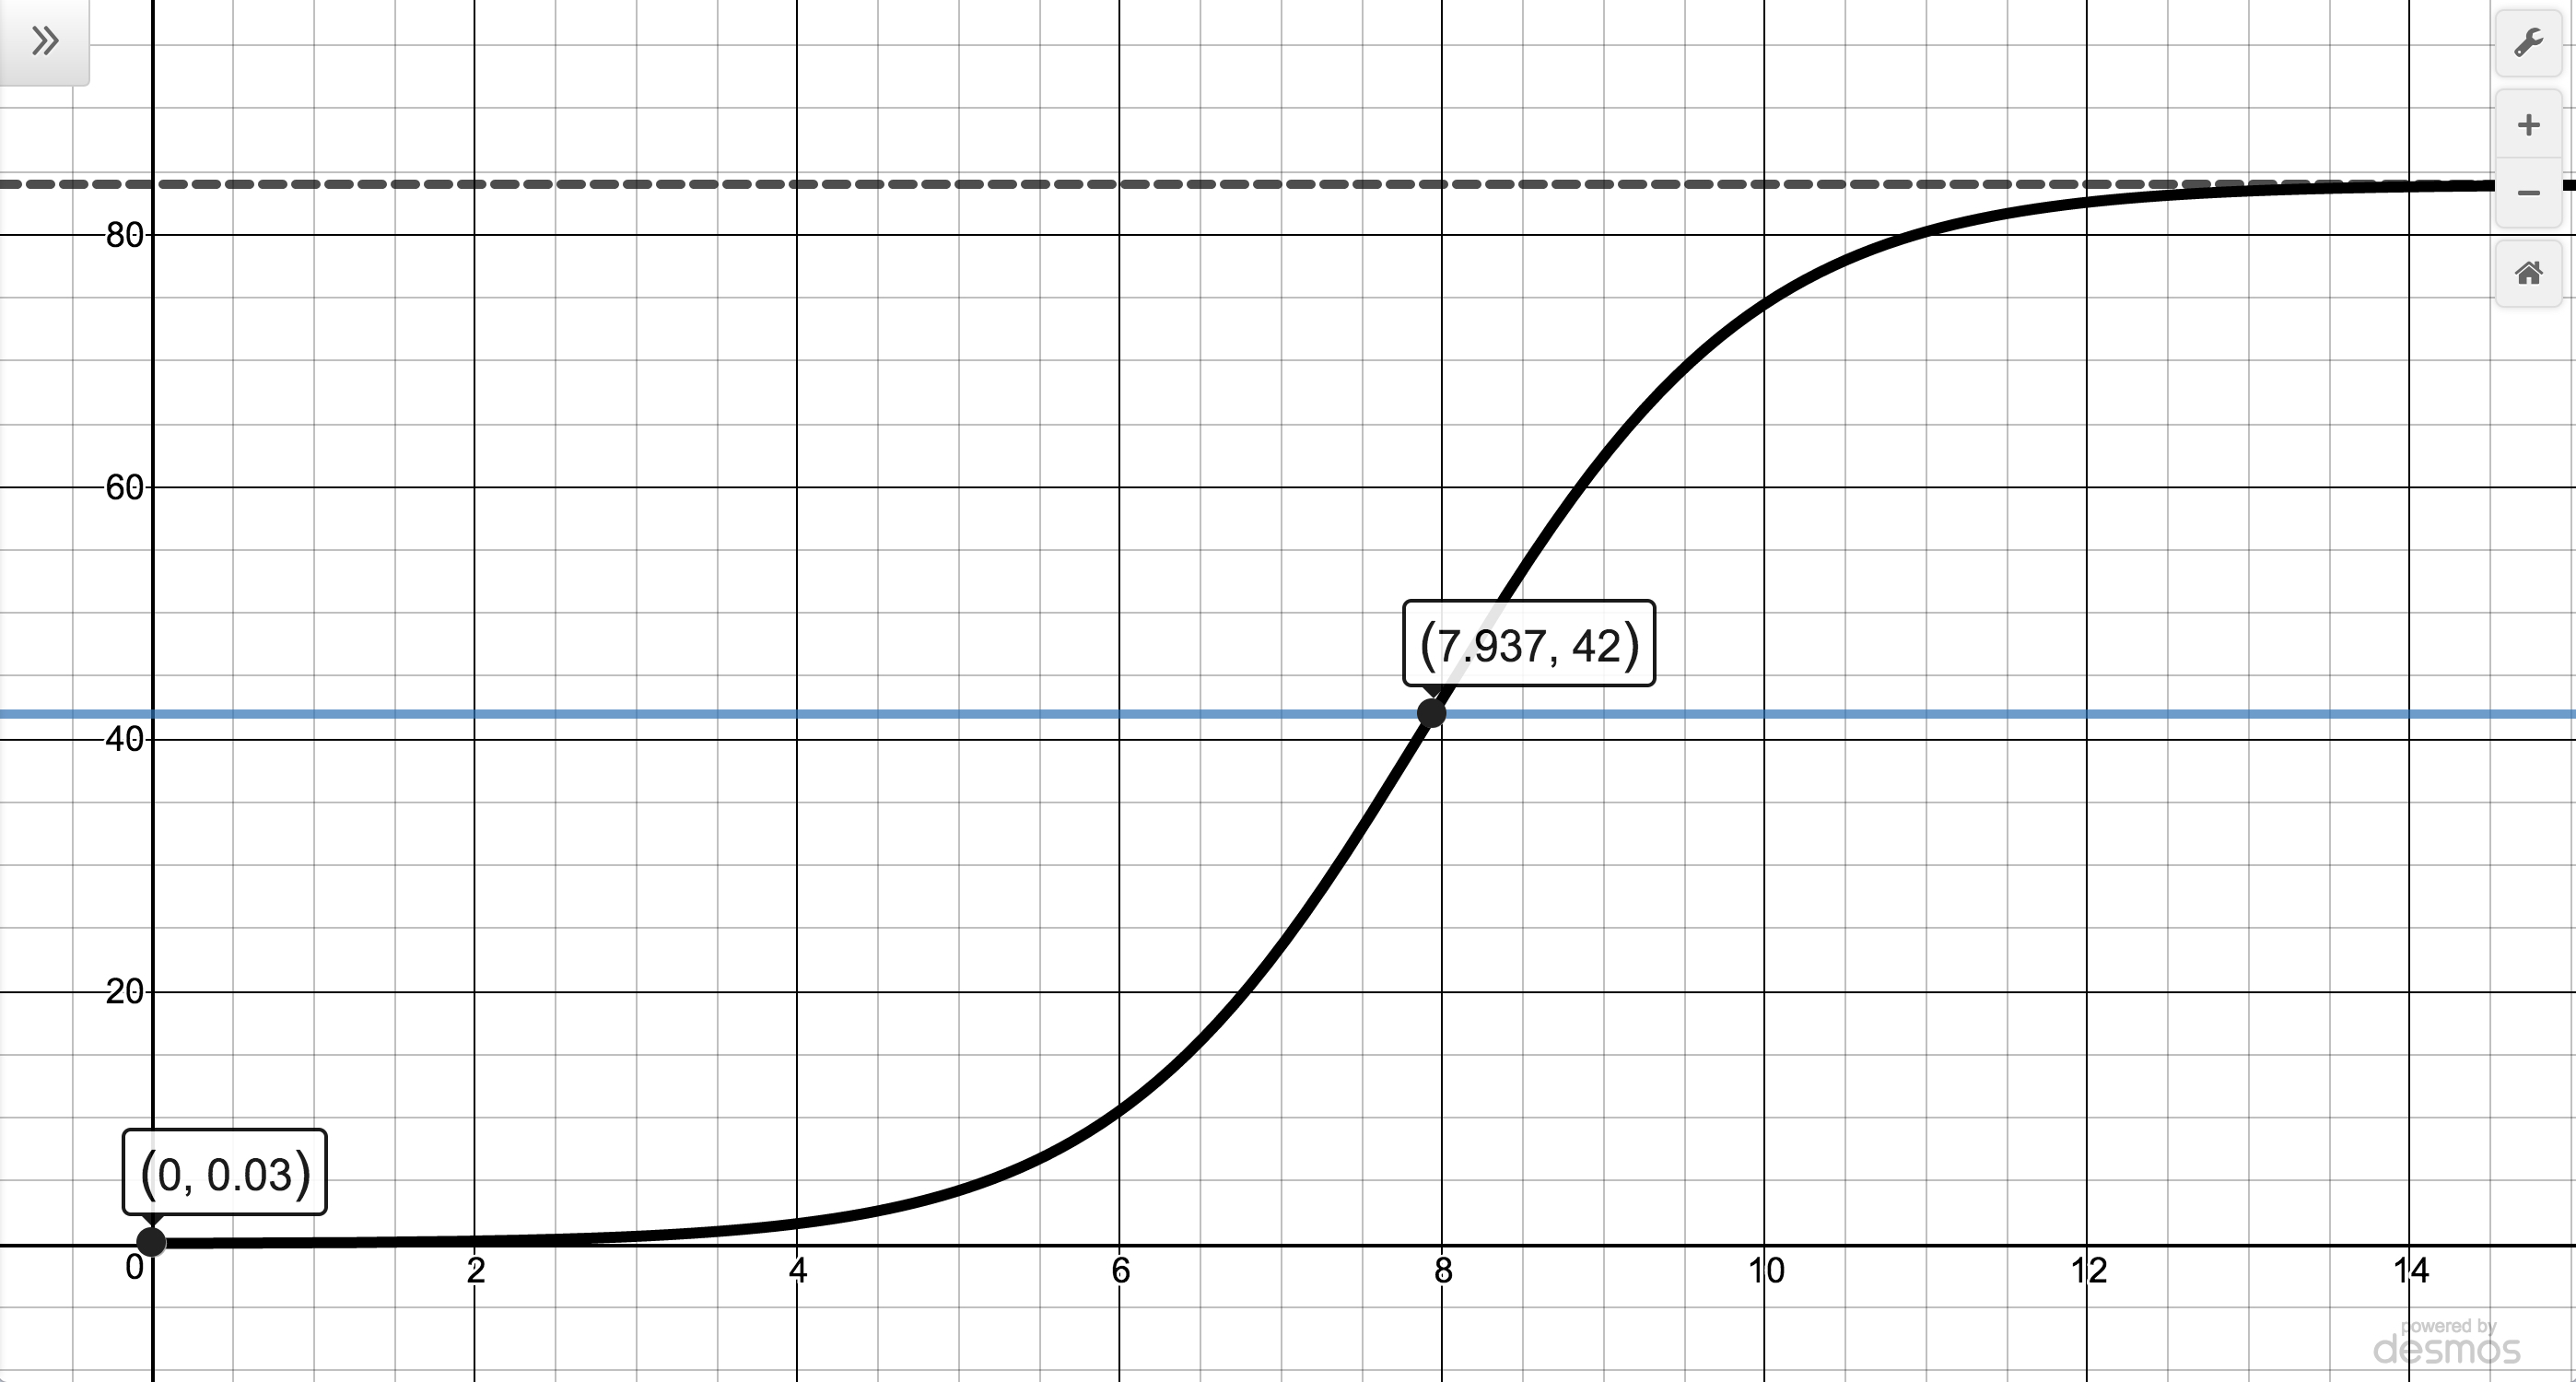
\includegraphics[width=4in]{./ApplicationsofExponentialandLogarithmicFunctionsGraphics/ExpLogAppEx01.jpg} 


\end{center}

\end{enumerate}

\qed

\end{ex}

If we take the time to analyze the graph of $y=N(t)$ in Example \ref{rumorex}, we can see \textit{graphically} how logistic growth combines  features of uninhibited and limited growth.  

\smallskip

The curve is concave up, rising steeply, then at some point, becomes concave down and begins to level off.\footnote{We introduced the notion of concavity in Section \ref{PowerFunctions}.}  The point at which this happens is called an \index{inflection point}\index{point of diminishing returns} \textbf{inflection point} or is sometimes called the `point of diminishing returns'.   Even though the function is still increasing through the inflection point, the \textit{rate} at which it does so begins to decrease. 

\smallskip

With Calculus, one can show the point of diminishing returns always occurs at half the limiting population.  (In our case, when $N(t)=42$.)  So with that in mind, we present two portions of the graph of $y=N(x)$, one on the interval $[0,8]$, the other on $[8,15]$. The former looks strikingly like uninhibited growth while the latter like limited growth.

\begin{center}

\begin{tabular}{cc}

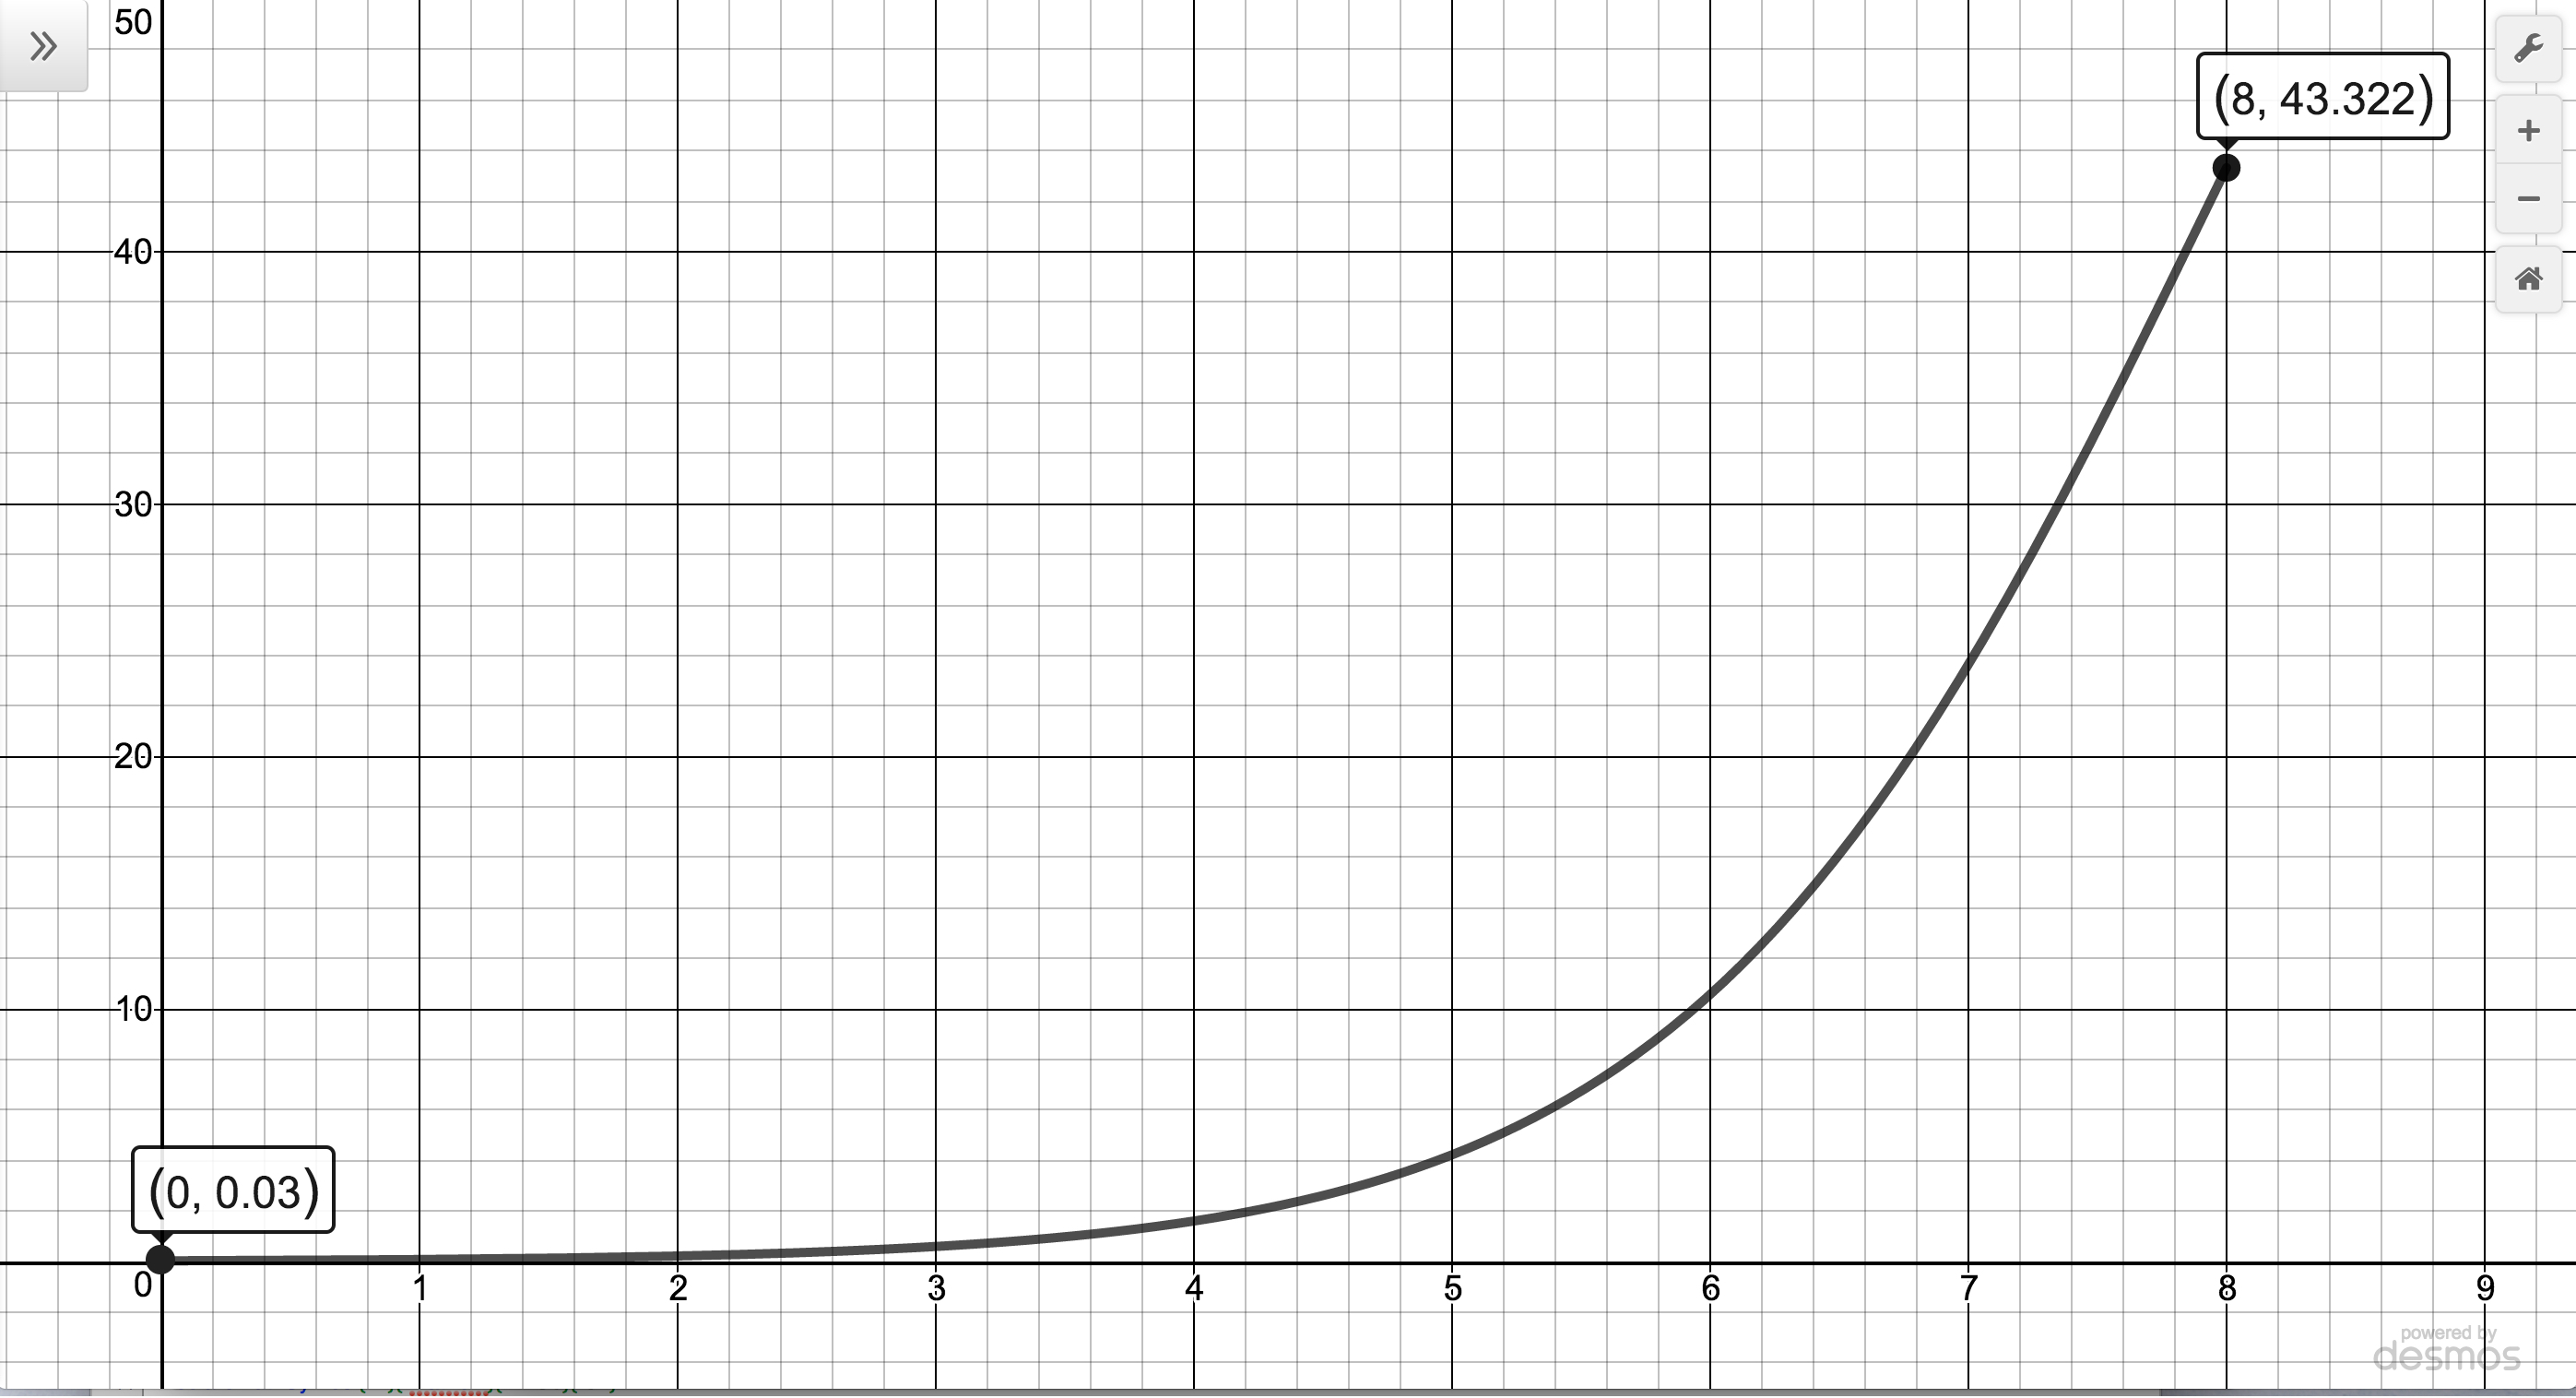
\includegraphics[width=3in]{./ApplicationsofExponentialandLogarithmicFunctionsGraphics/ExpLogAppEx02.jpg} &

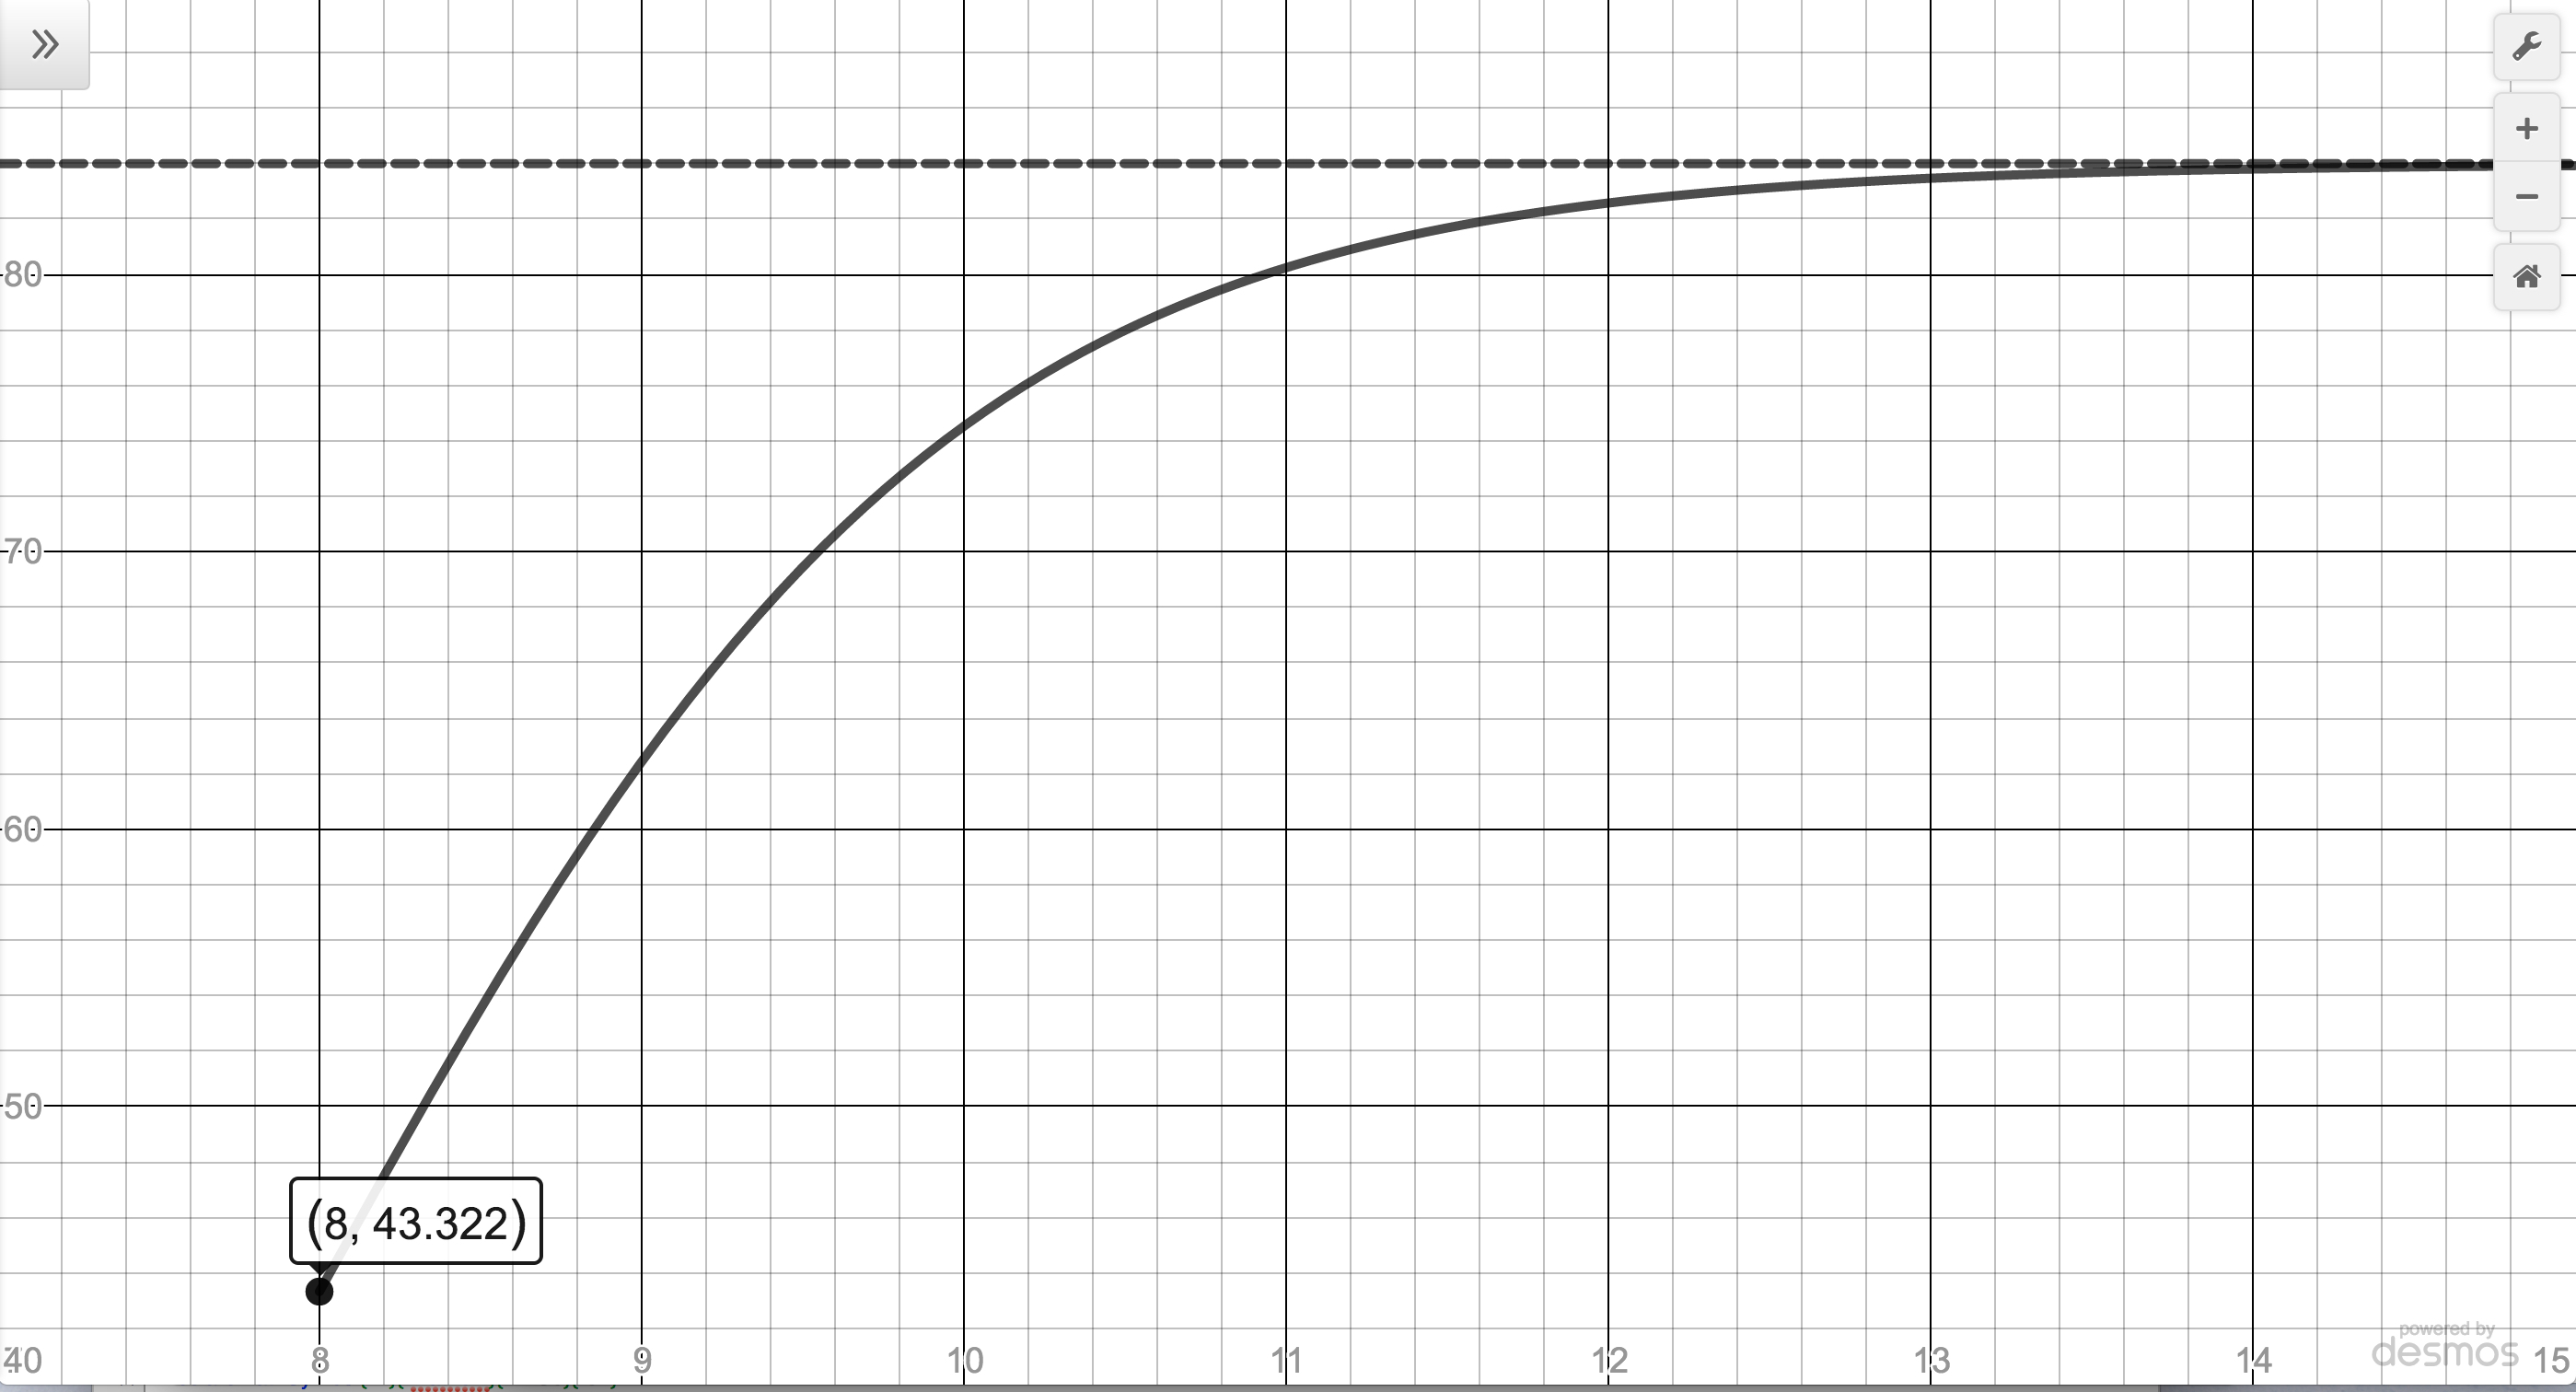
\includegraphics[width=3in]{./ApplicationsofExponentialandLogarithmicFunctionsGraphics/ExpLogAppEx03.jpg} \\

$y = N(t)$ for $0 \leq t \leq 8$ &

$y = N(t)$ for $8 \leq t \leq 15$

\end{tabular}

\end{center}


\subsection{Applications of Logarithms}

Just as many physical phenomena can be modeled by exponential functions, the same is true of logarithmic functions.   In Exercises \ref{Richterexercise},  \ref{decibelexercise} and \ref{pHexercise} of Section \ref{LogarithmicFunctions}, we showed that logarithms are useful in measuring the intensities of earthquakes (the Richter scale), sound (decibels) and acids and bases (pH).  We now present yet a different use of the a basic logarithm function, \href{http://en.wikipedia.org/wiki/Password_strength}{\underline{password strength}}.

\smallskip

\begin{ex}  The \href{http://en.wikipedia.org/wiki/Information_entropy}{\underline{information entropy}} $H$, in bits, of a randomly generated password consisting of $L$ characters is given by $H = L \log_{2}(N)$, where $N$ is the number of possible symbols for each character in the password.  In general, the higher the entropy, the stronger the password. \index{password strength} \index{information entropy}

\begin{enumerate}

\item  If a $7$ character case-sensitive\footnote{That is, upper and lower case letters are treated as different characters.} password is comprised of  letters and numbers only, find the associated information entropy.

\item  How many possible symbol options per character is required to produce a $7$ character password with an information entropy of $50$ bits?

\end{enumerate}

{\bf Solution.}

\begin{enumerate}

\item  There are $26$ letters in the alphabet, $52$ if upper and lower case letters are counted as different.  There are $10$ digits ($0$ through $9$) for a total of $N=62$ symbols.  Since the password is to be $7$ characters long, $L = 7$.  Thus, $H = 7 \log_{2}(62) = \frac{7 \ln(62)}{\ln(2)} \approx 41.68$.

\item  We have $L = 7$ and $H=50$ and we need to find $N$.  Solving the equation $50 = 7 \log_{2}(N)$ gives $N = 2^{50/7} \approx 141.323$, so we would need $142$ different symbols to choose from.\footnote{Since there are only $94$ distinct ASCII keyboard characters, to achieve this strength, the number of characters in the password should be increased.} \qed

\end{enumerate}

\end{ex}

\smallskip

Chemical systems known as \href{http://en.wikipedia.org/wiki/Buffer_solutions}{\underline{buffer solutions}} \index{buffer solution} have the ability to adjust to small changes in acidity to maintain a range of pH values.  Buffer solutions have a wide variety of applications from maintaining a healthy fish tank to regulating the pH levels in blood.  Our next example shows how the pH in a buffer solution is a little more complicated than the pH we first encountered in Exercise \ref{pHexercise} in Section \ref{LogarithmicFunctions}. 

\smallskip

\begin{ex}  Blood is a buffer solution. When carbon dioxide is absorbed into the bloodstream it produces carbonic acid and lowers the pH.  The body compensates by producing bicarbonate, a weak base to partially neutralize the acid.   The equation\footnote{Derived from the \href{http://en.wikipedia.org/wiki/Henderson-Hasselbalch_equation}{\underline{Henderson-Hasselbalch Equation}}. See Exercise \ref{HendersonHasselbalch} in Section \ref{PropertiesofLogarithms}.  Hasselbalch himself was studying carbon dioxide dissolving in blood - a process called \href{http://en.wikipedia.org/wiki/Metabolic_acidosis}{\underline{metabolic acidosis}}.}   which models blood pH in this situation is $\mbox{pH} = 6.1 + \log\left(\frac{800}{x} \right)$, where $x$ is the partial pressure of carbon dioxide in arterial blood, measured in torr. Find the partial pressure of carbon dioxide in arterial blood if the pH is $7.4$.

\smallskip

{\bf Solution.}  We set $\mbox{pH} = 7.4$ and get $ 7.4 = 6.1 + \log\left(\frac{800}{x} \right)$, or $\log\left(\frac{800}{x} \right) = 1.3$.   We get $x = \frac{800}{10^{1.3}} \approx 40.09$.  Hence, the partial pressure of carbon dioxide in the blood is about $40$ torr. \qed


\end{ex}

Another place logarithms are used is in data analysis. Suppose, for instance, we wish to model the spread of influenza A (H1N1), the so-called `Swine Flu'.  Below is data taken from the World Health Organization (\href{http://www.who.int/csr/disease/swineflu/updates/en/index.html}{\underline{WHO}}) where $t$ represents the number of days since April 28, 2009, and $N$ represents the number of confirmed cases of H1N1 virus worldwide.

\[ \begin{array}{|c||c|c|c|c|c|c|c|c|c|c|c|c|c|}  \hline

t & 1 & 2 & 3 & 4 & 5 & 6 & 7 & 8 & 9 & 10 & 11 & 12 & 13  \\ \hline

N & 148 & 257 &   367 & 658 & 898 & 1085 & 1490 & 1893 & 2371 & 2500 & 3440 & 4379 & 4694  \\ \hline \end{array} \]


\[\begin{array}{|c||c||c|c|c|c|c|c|} \hline

t & 14 & 15 & 16 & 17 & 18 & 19& 20  \\ \hline 

N & 5251 & 5728 & 6497 & 7520 & 8451 & 8480 & 8829    \\ \hline \end{array} \]

Making a scatter plot of the data treating $t$ as the independent variable and $N$ as the dependent variable gives the plot below on the left.  Which models are suggested by the shape of the data?  

\smallskip

Thinking back Section \ref{QuadraticFunctions}, we try a Quadratic Regression.  We find $N(t) \approx 16.713 t^2 +149.68t -233.15$ with $R^2 = 0.992$, indicating a pretty good fit.  However, is there any underlying scientific principle which would account for these data to be quadratic?  Are there other models which fit the data  better?


\begin{center}

\begin{tabular}{cc}

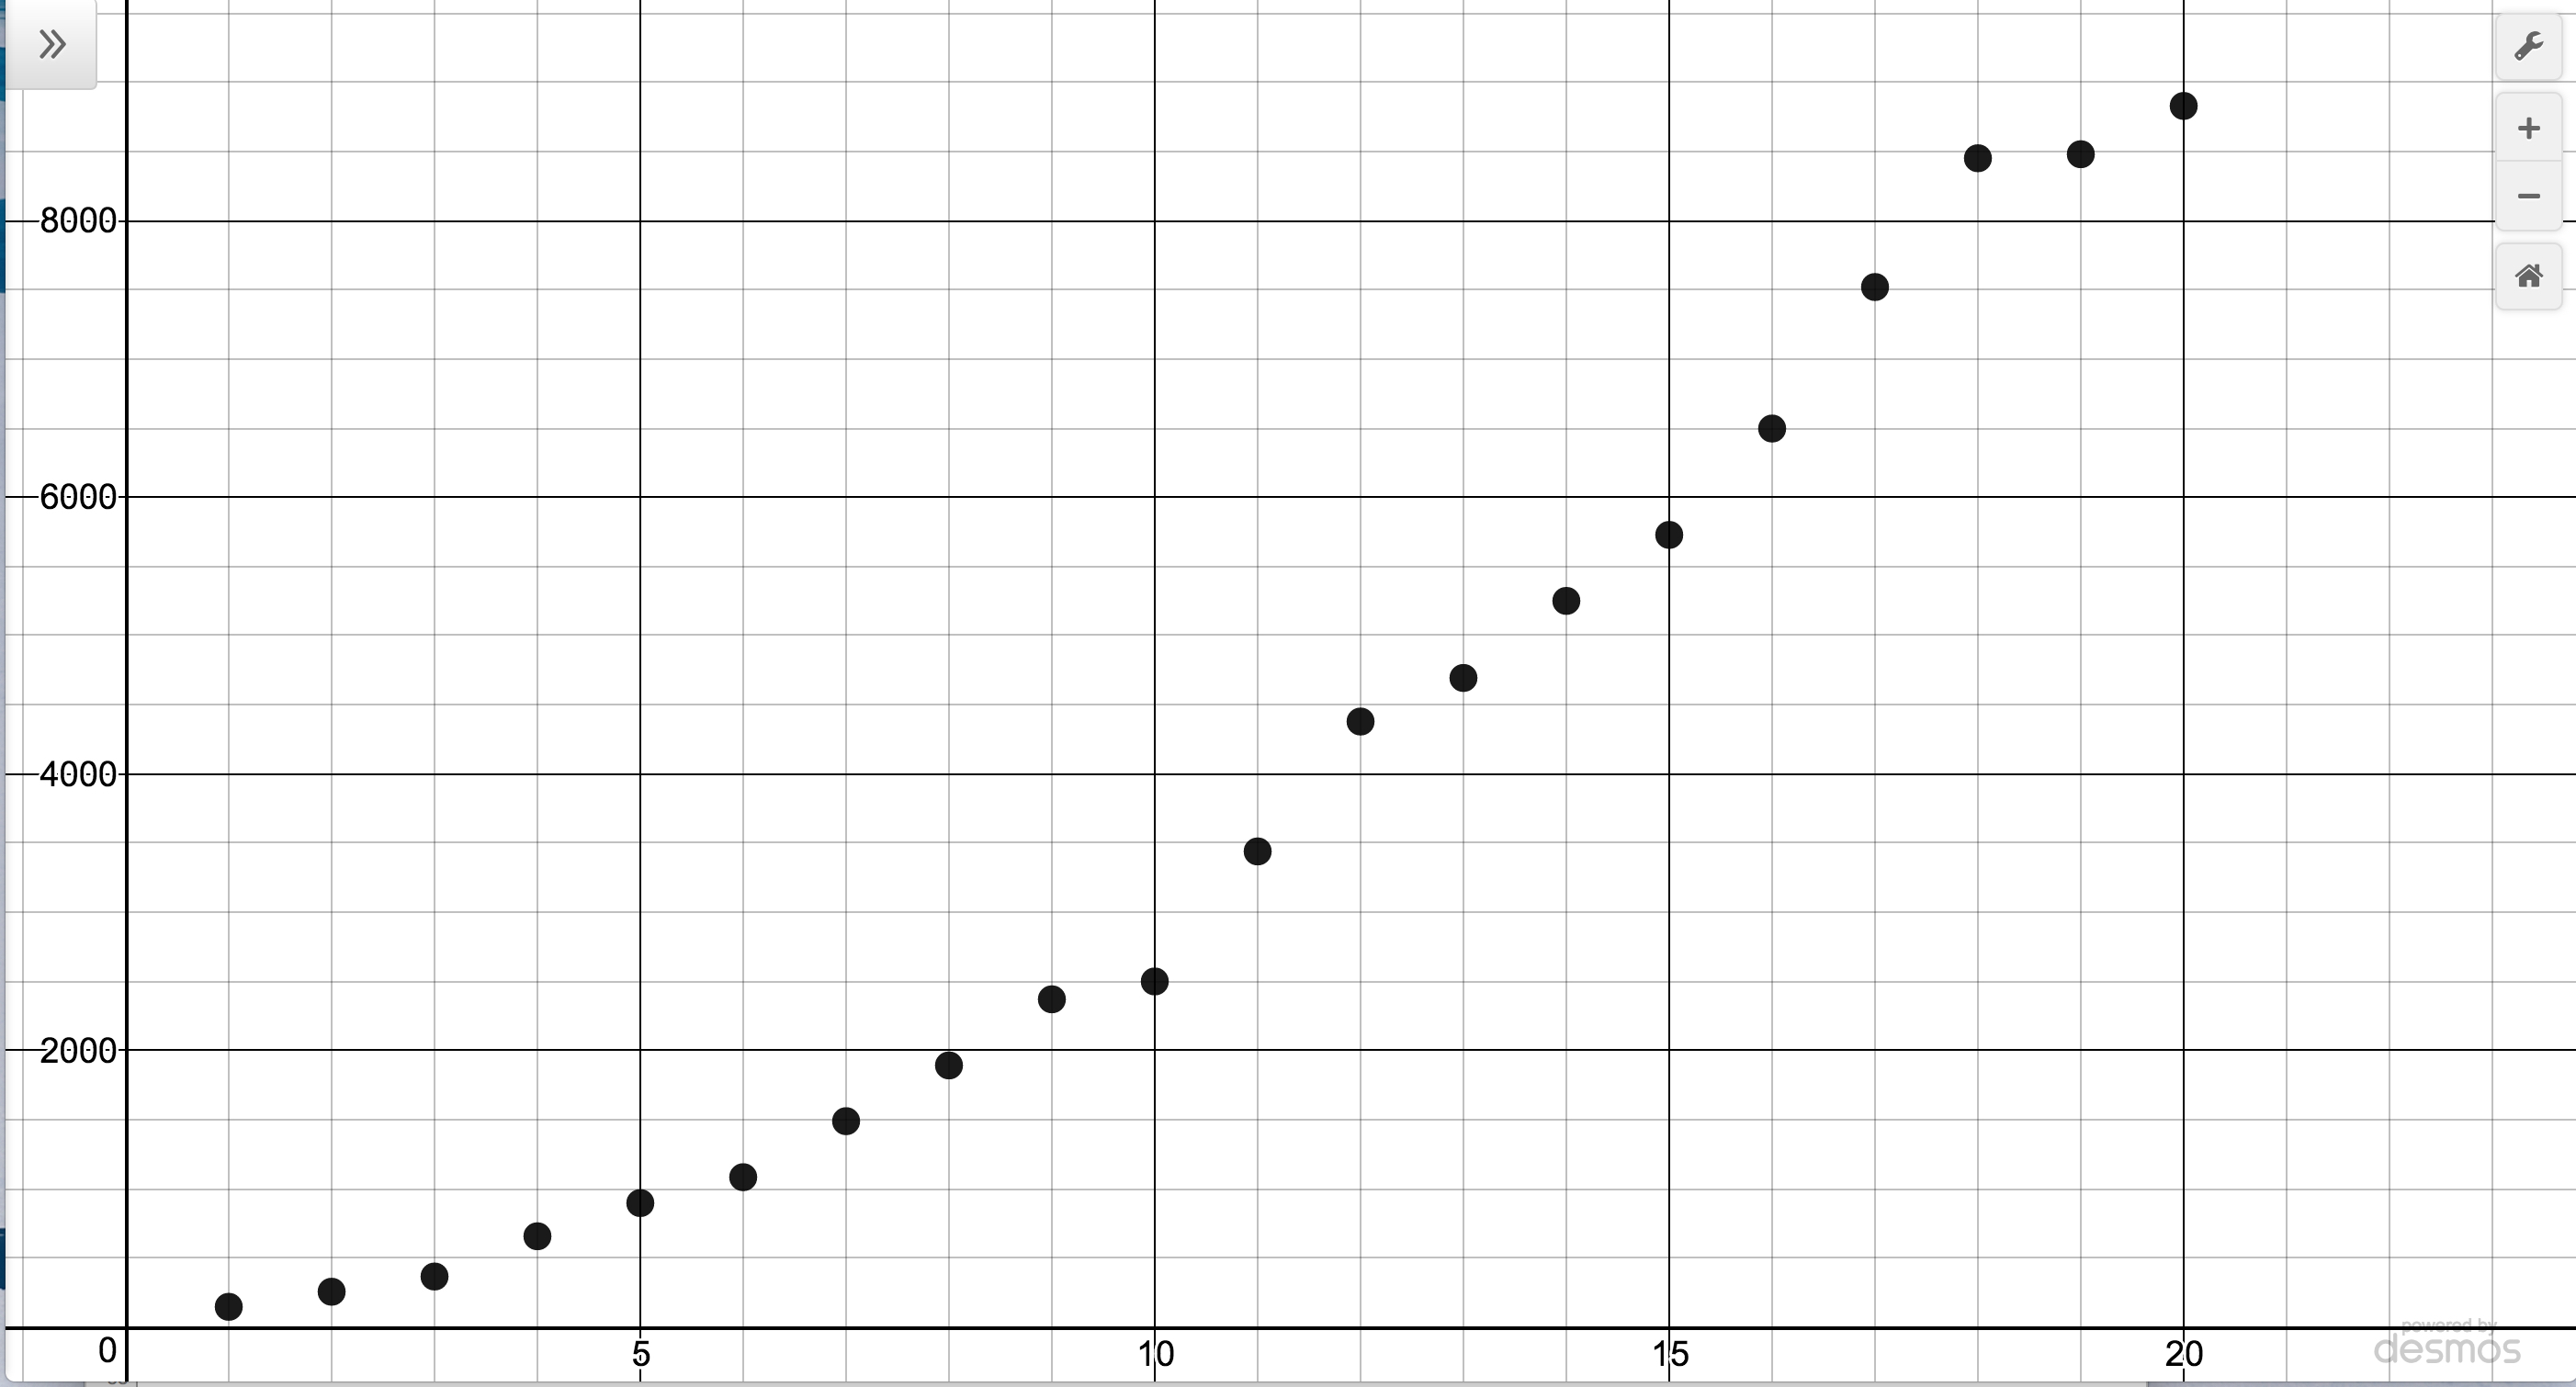
\includegraphics[width=3in]{./ApplicationsofExponentialandLogarithmicFunctionsGraphics/ExpLogAppEx04.jpg} &

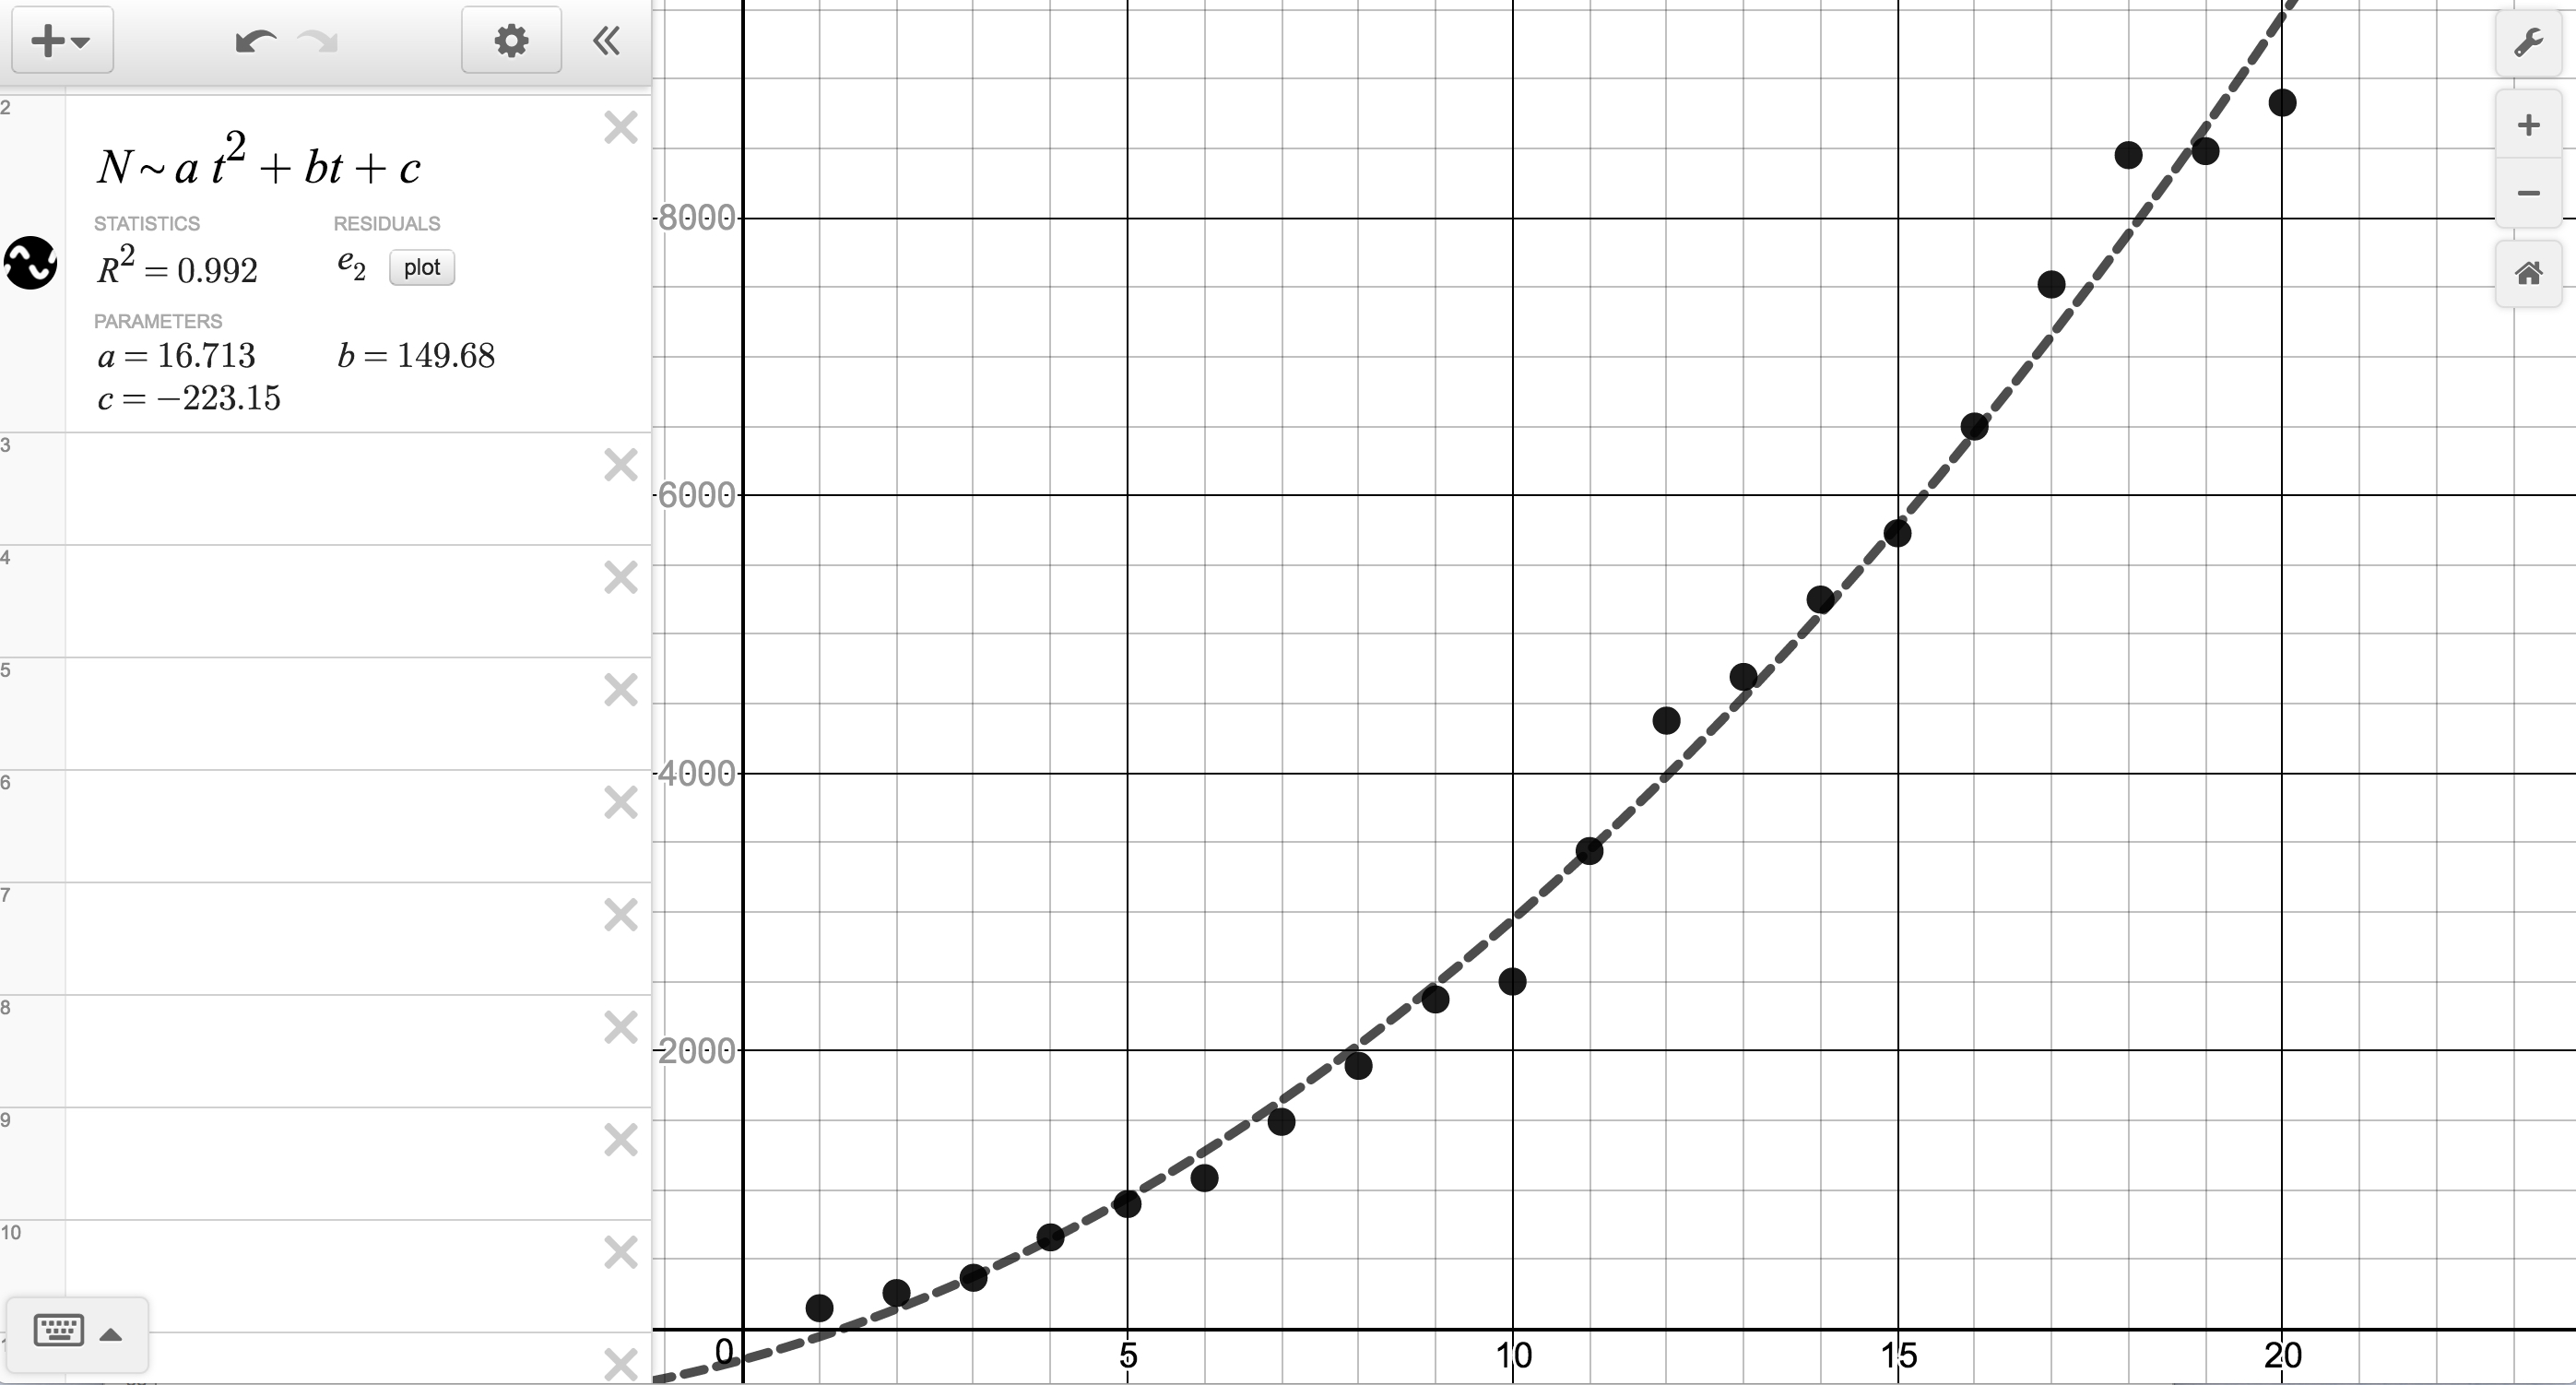
\includegraphics[width=3in]{./ApplicationsofExponentialandLogarithmicFunctionsGraphics/ExpLogAppEx05.jpg} \\

Scatterplot of the Data &

A quadratic regression model \\

\end{tabular}

\end{center}

To answer these questions, scientists often use logarithms in an attempt to `linearize' non-liner data sets such as the one before us.  To see how this could work, suppose we guessed the relationship between $N$ and $t$ is something from Section \ref{PowerFunctions},  $N(t) = a t^{p}$.  

\smallskip

By taking the natural logs of both sides and using the Product and Power Rules, in turn, we find that $\ln(N(t)) = \ln(a t^p) = \ln(a) + \ln(t^p) = \ln(a) + p \ln(t) =  p \ln(t) + \ln(a)$.   If we let  $x = \ln(t)$ and $y= \ln(N(t))$,  the model takes the form $y = p x + \ln(a)$ which is a \textit{linear} model with slope $p$ and $y$-intercept $\ln(a)$.  So, instead of plotting $N(t)$ versus $t$, we plot $y=\ln(N(t))$ versus $x=\ln(t)$ and find a linear regression for this data set.

\[ \begin{array}{|c||c|c|c|c|c|c|c|c|c|c|c|c|c|}  \hline

\ln(t) & 0 & 0.693 & 1.099 & 1.386& 1.609 & 1.792 & 1.946 & 2.079 & 2.197 & 2.302 & 2.398 & 2.485 & 2.565  \\ \hline

\ln(N) & 4.997  & 5.549 &  5.905 & 6.489 & 6.800 & 6.989 & 7.306 & 7.546 & 7.771 & 7.824 & 8.143 & 8.385 & 8.454  \\ \hline \end{array} \]


\[\begin{array}{|c||c||c|c|c|c|c|c|} \hline

\ln(t) & 2.639 & 2.708 & 2.773 & 2.833 & 2.890 & 2.944 & 2.996  \\ \hline 

\ln(N) & 8.566 & 8.653 & 8.779 & 8.925 & 9.042 & 9.045 & 9.086    \\ \hline \end{array} \]

\begin{center}

\begin{tabular}{cc}

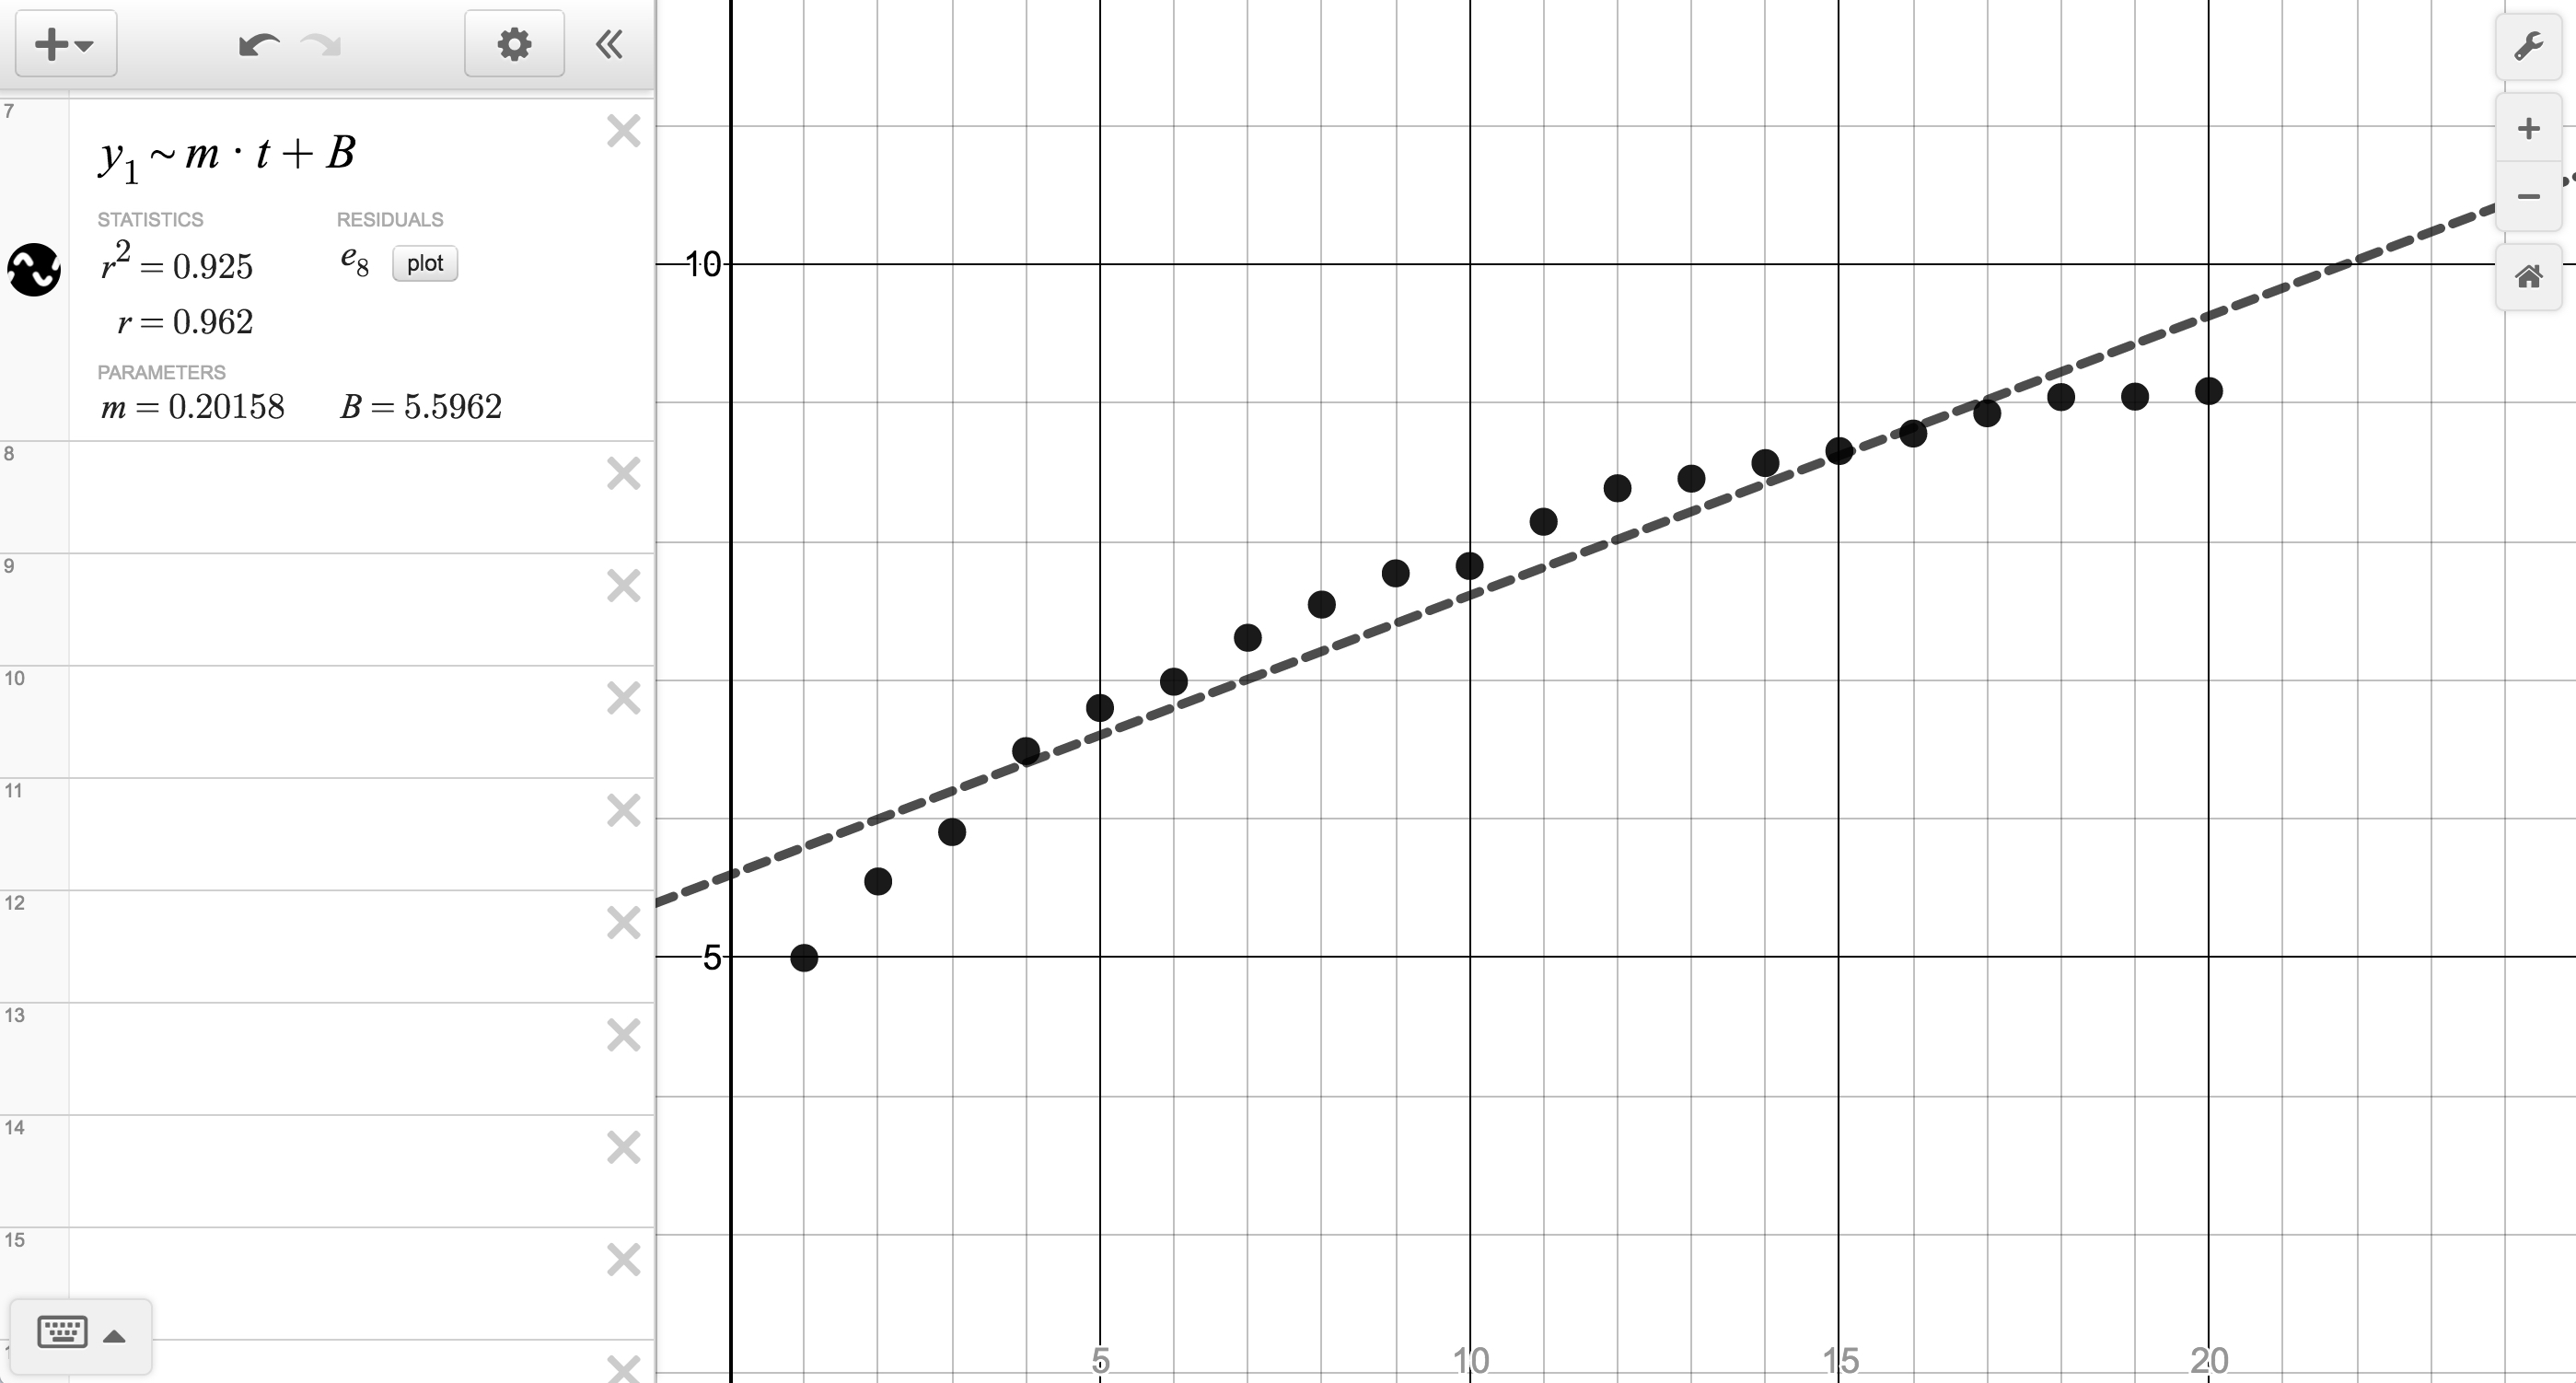
\includegraphics[width=3in]{./ApplicationsofExponentialandLogarithmicFunctionsGraphics/ExpLogAppEx10.jpg} &

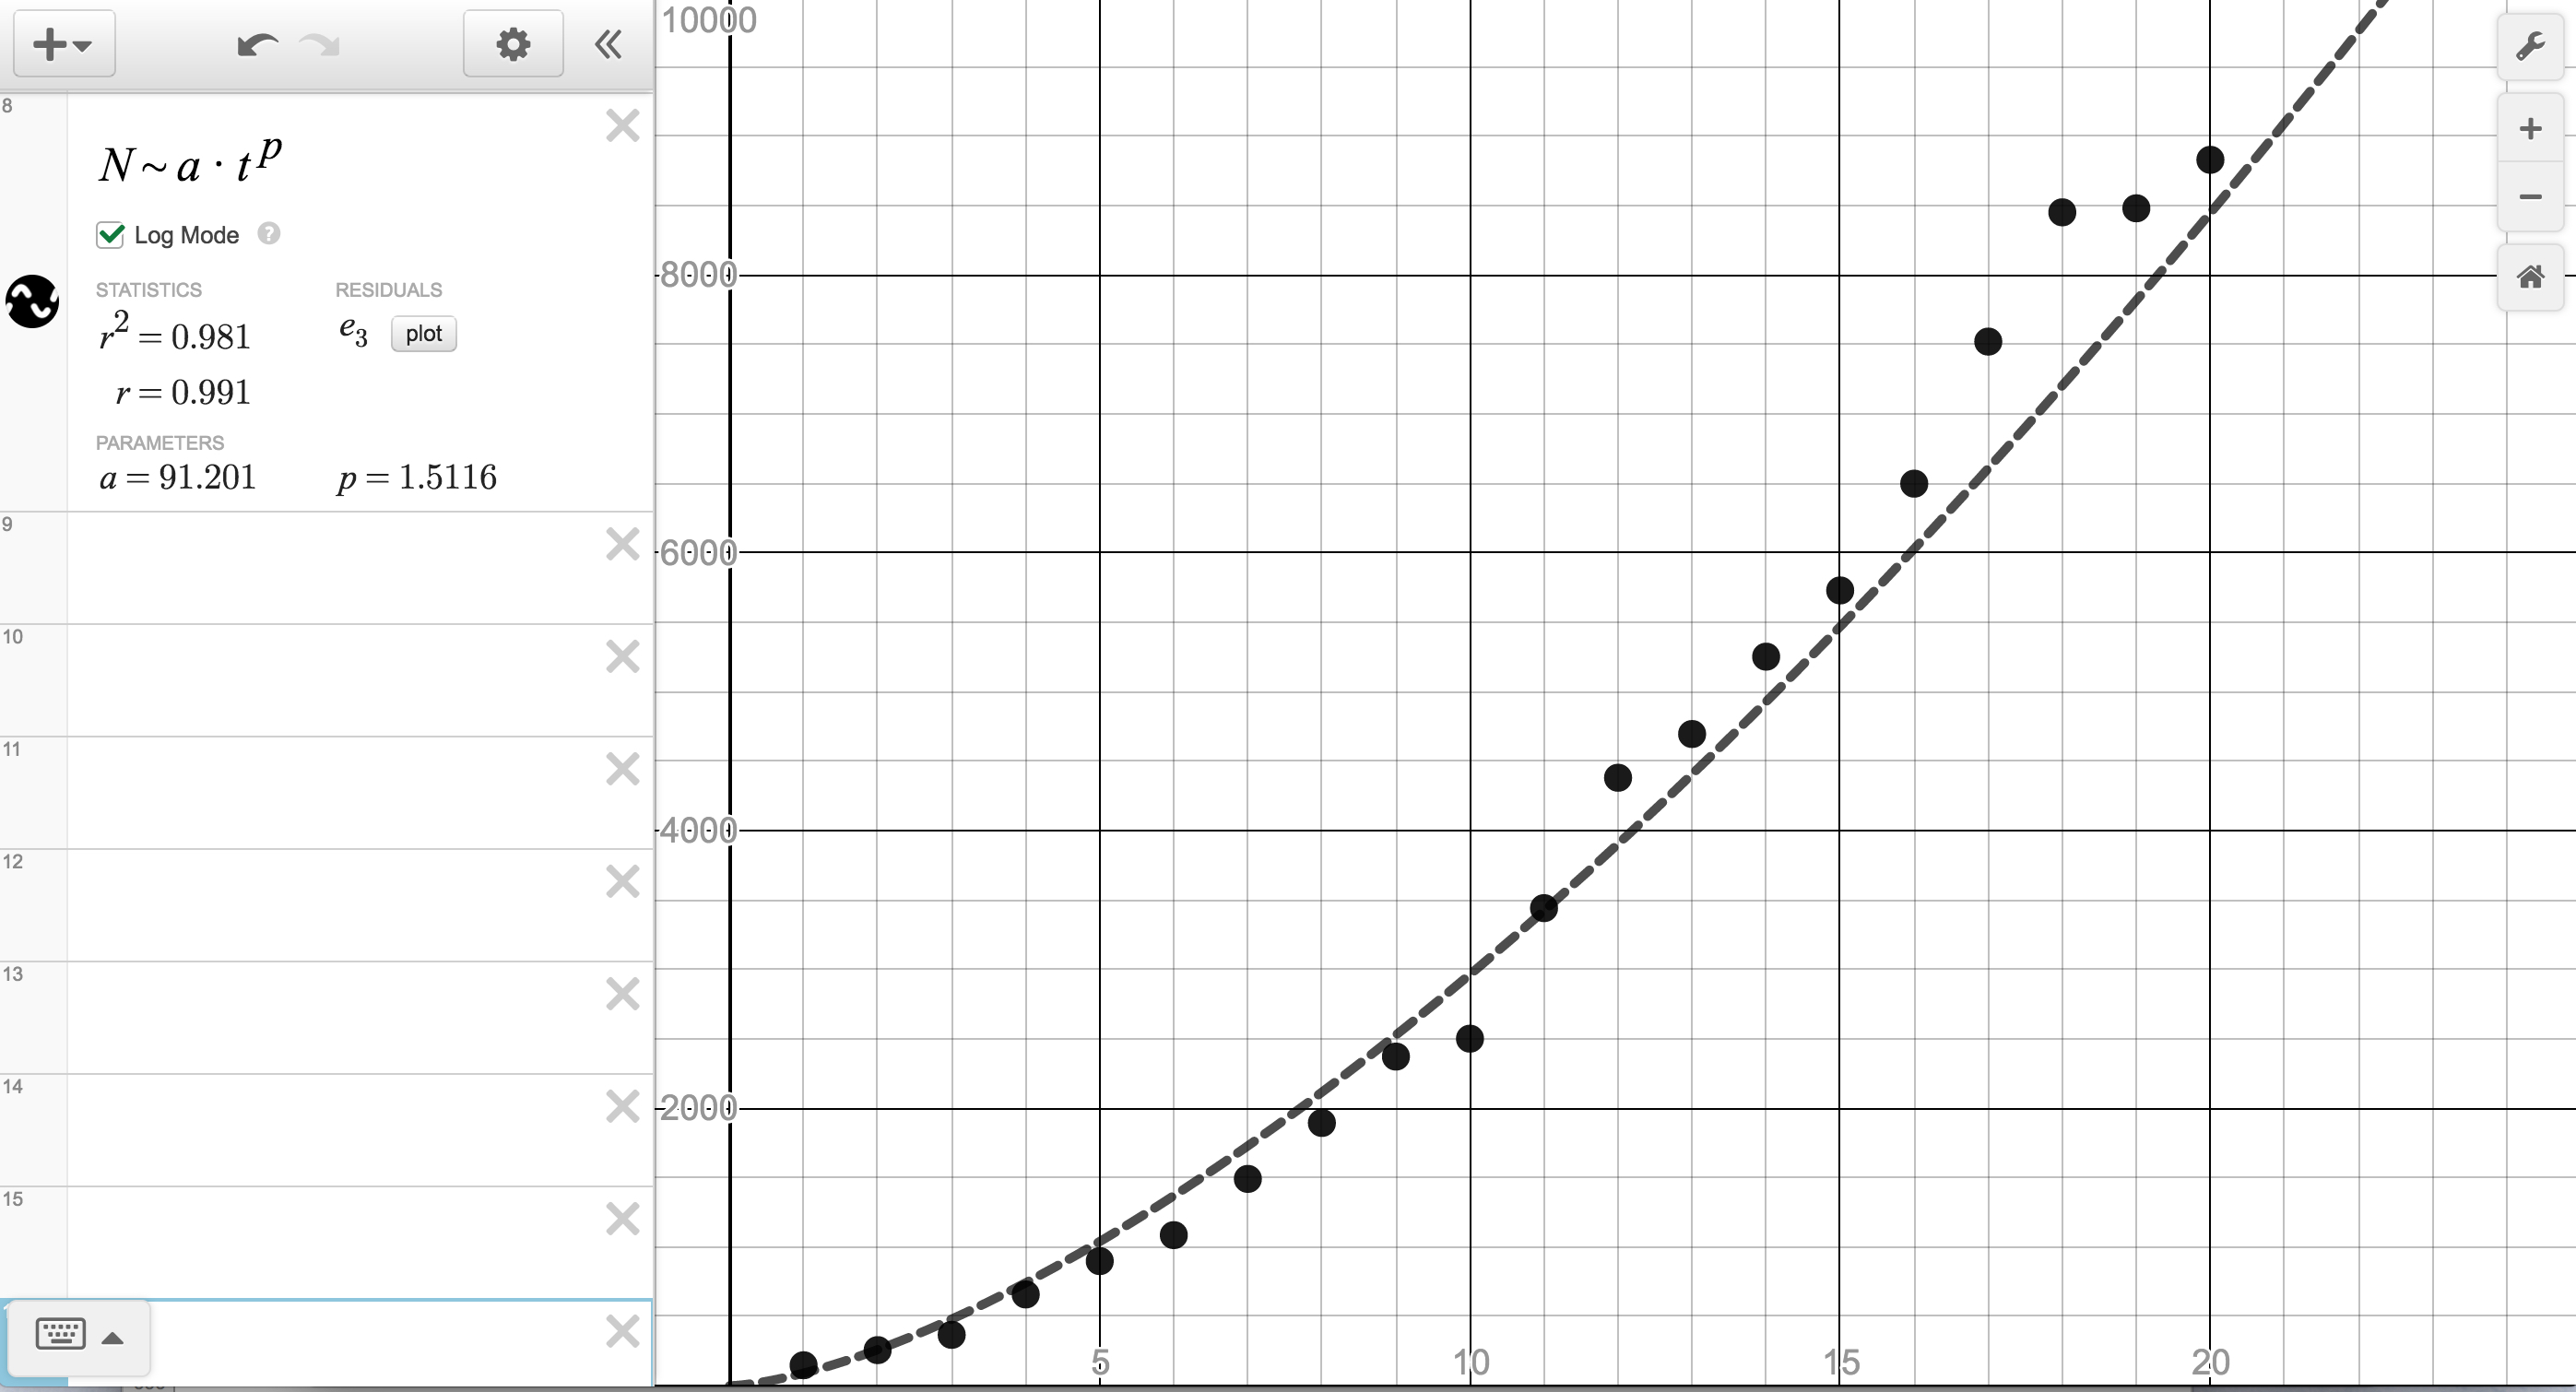
\includegraphics[width=3in]{./ApplicationsofExponentialandLogarithmicFunctionsGraphics/ExpLogAppEx06a.jpg} \\

linear regression: $\ln(N(t)) = p \ln(t) + \ln(a)$ &

power function regression: $N(t) = at^{p}$ \\

\end{tabular}

\end{center}



We see $r=0.991$, which is very close to $1$ indicating a very good fit.   The slope of the regression line is $m \approx 1.512$ which corresponds to our exponent $p$.  The $y$-intercept $b \approx 4.513$ corresponds to $\ln(a)$, so that $a \approx 91.201$.  Hence, we get the model $N = 91.201 t^{1.512}$. 

\smallskip

Of interest here is that the graphing utility we used, \href{https://www.desmos.com}{\underline{desmos}} has its own built-in power regression model.  If the `log mode'  square is checked, the graphing utility returns the \textit{same} model we obtained using our linearization (since the routine which determines the coefficients uses logarithms as well.)\footnote{If, however, we uncheck that box, we get a \textit{different} power function model, $N(t) = 62.318 t^{1.675}$ which chooses $a$ and $p$ directly to minimize the total squared error.  See \href{http://support.desmos.com/hc/en-us/articles/204349605}{\underline{here}} for more details.}

\smallskip

At this point, the quadratic model fits the data better, ostensibly because we have \textit{three} parameters we can adjust in the formula $N(t) = at^2+bt+c$ to minimize our error as opposed to just \textit{two} parameters in the formula $N(t) = a t^{p}$.  Neither  model, however, is based on any underlying scientific principle.

\smallskip

If we think about this situation from a scientific perspective, it does seem to make sense that, at least in the early stages of the outbreak, the more people who have the flu, the faster it will spread.  This suggests we fit the data to an uninhibited growth model.

\smallskip

As  written,  Equation \ref{lawofuninhibitedgrowth} gives uninhibited growth as  $N(t) = N_{\mbox{\tiny$0$}}e^{kt}$. Here, for simplicity's sake, we relabel $N_{\mbox{\tiny$0$}} = a$ and $e^{k} = b$ so that we are looking for parameters $a$ and $b$ so that $N(t) = a \cdot b^{t}$.

\smallskip

\phantomsection
\label{swineflulinearized}
If we assume $N(t) = a \cdot b^{t}$ then, taking logs as before, we get $\ln(N(t)) = t \ln(b) + \ln(a)$. If we let $y= \ln(N(t))$, then, once again, we get a linear model this time with slope $\ln(b)$ and $y$-intercept $\ln(a)$.  We present the results of the regression below.  While there is a strong correlation, $r = 0.962$, the plot doesn't instill the greatest of confidence in this model.

\begin{center}

\begin{tabular}{cc}

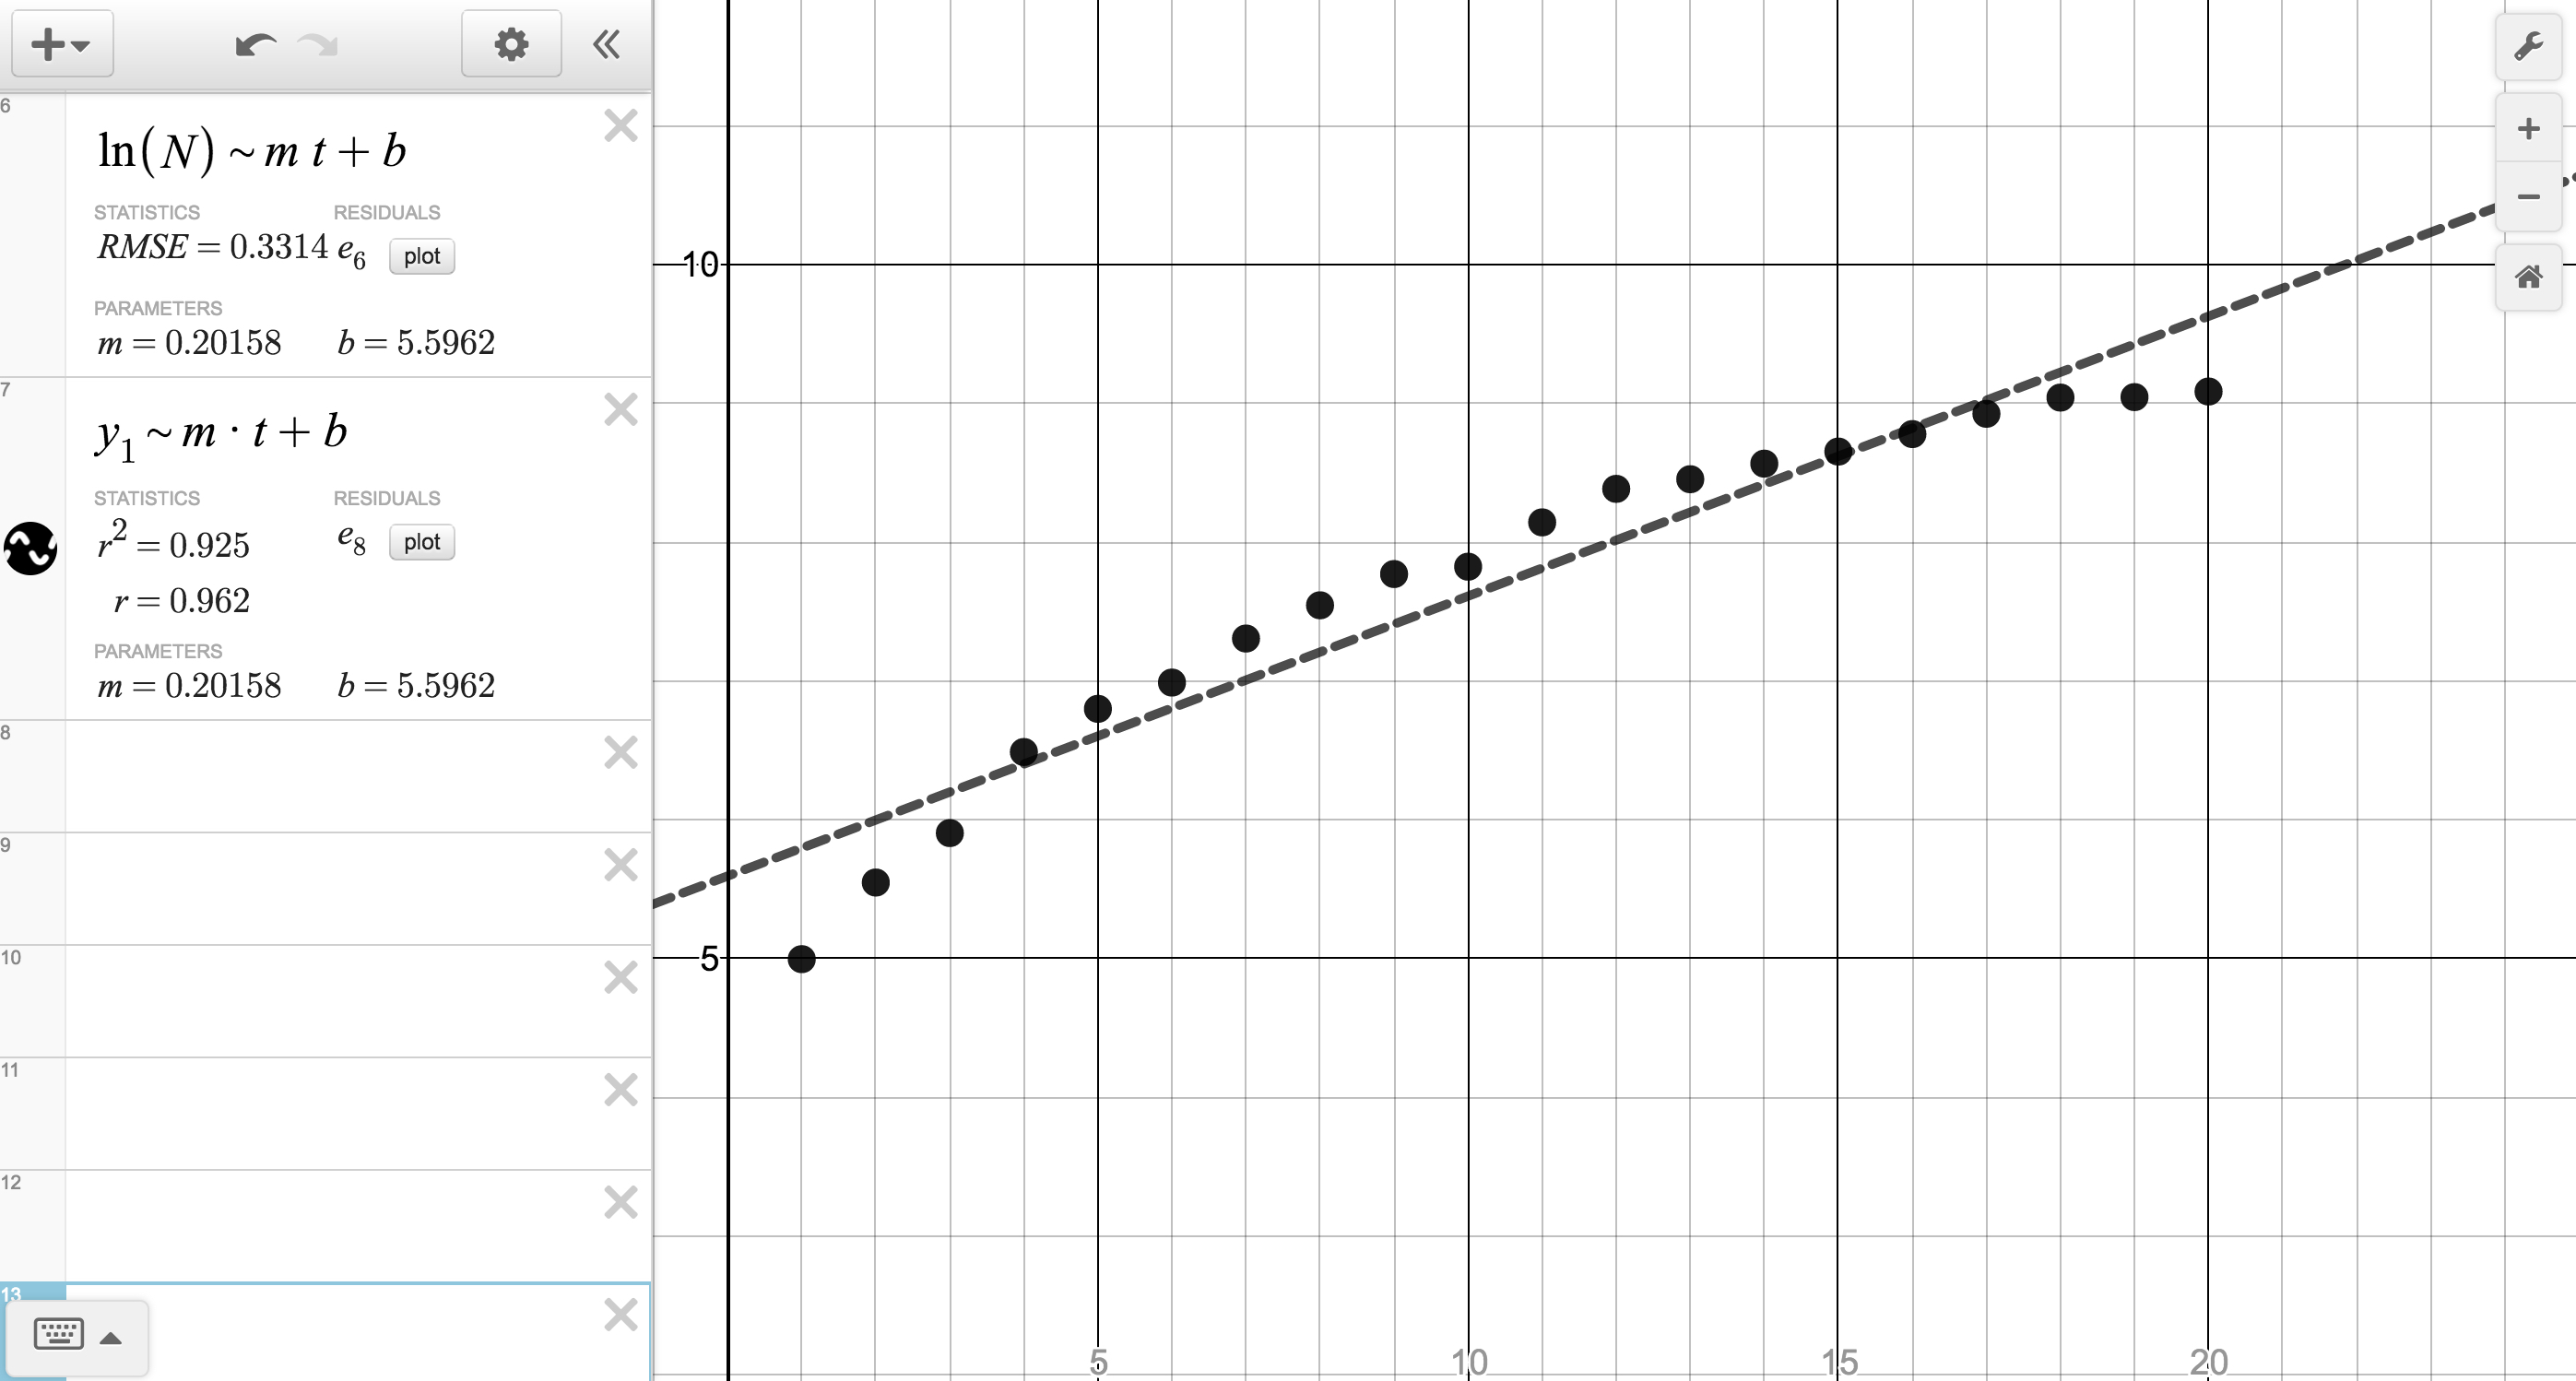
\includegraphics[width=3in]{./ApplicationsofExponentialandLogarithmicFunctionsGraphics/ExpLogAppEx09.jpg} &

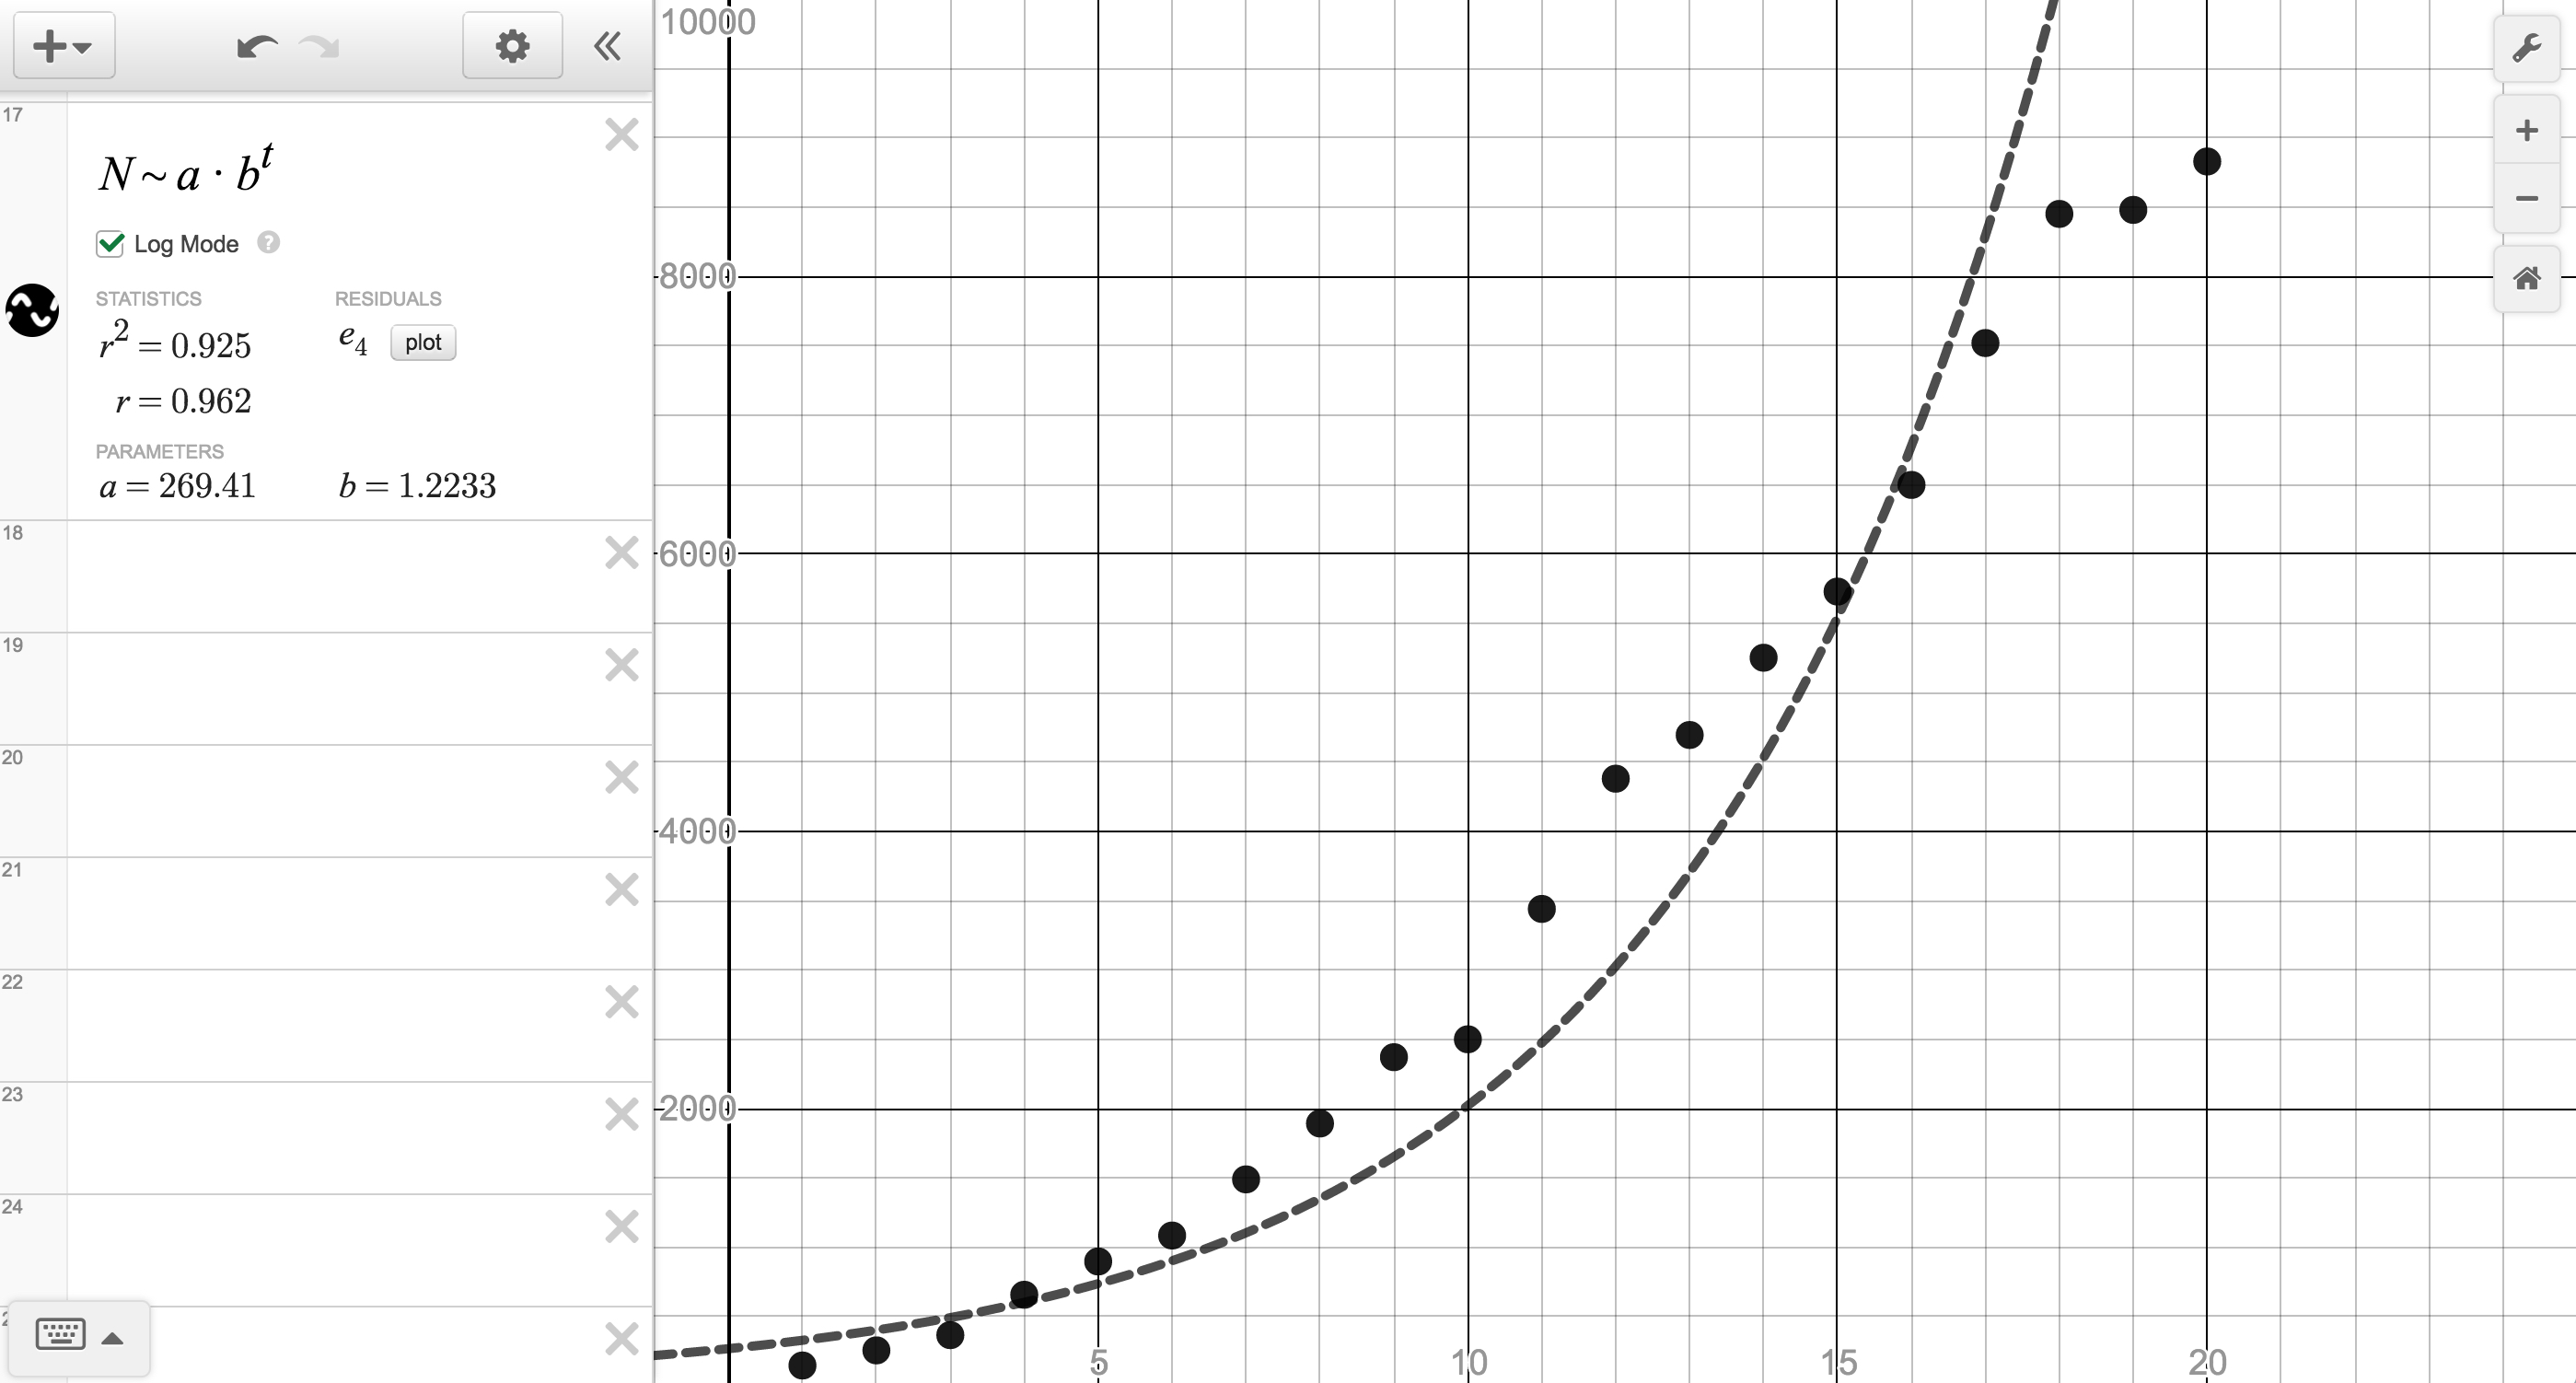
\includegraphics[width=3in]{./ApplicationsofExponentialandLogarithmicFunctionsGraphics/ExpLogAppEx07a.jpg} \\

linear regression: $\ln(N(t)) = t \ln(b) + \ln(a)$ &

exponential regression: $N(t) = a \cdot b^{t}$ \\

\end{tabular}

\end{center}

From the slope of the model, we have   $m = \ln(b) \approx 0.202$  so $b \approx 1.223$.  From the $y$-intercept of the model, we get $B = \ln(a) \approx  5.596$ so $a \approx 269.35$, so that our model is $N(t) = 269.35(1.223)^{t}$. Using the built-in exponential regression (again, with `log mode' checked) returns the model  $N(t) = 269.41 (1.223)^{t}$, the discrepancy between   $269.35$ and $269.41$ stemming ostensibly from round-off error.    

\smallskip

The exponential model didn't fit the data as well as the quadratic or power function model, but it stands to reason that, perhaps, the spread of the flu is not unlike that of the spread of a rumor and that a logistic model can be used to model the data.  Again, for simplicity, we abbreviate the model given in Equation \ref{logisticgrowth} from $N(t) =\frac{L}{1 + Ce^{-kLt}}$ to $N(t) = \frac{L}{1 + Ce^{Kt}}$.

\smallskip

Running the data, a logistic function appears to be an excellent fit, both judging by the graph as well as the coefficient of determination, $R^2 \approx 0.995$.  Moreover, the underlying principles which lead to the formulation of this model seem reasonable enough.




 
 \begin{center}
 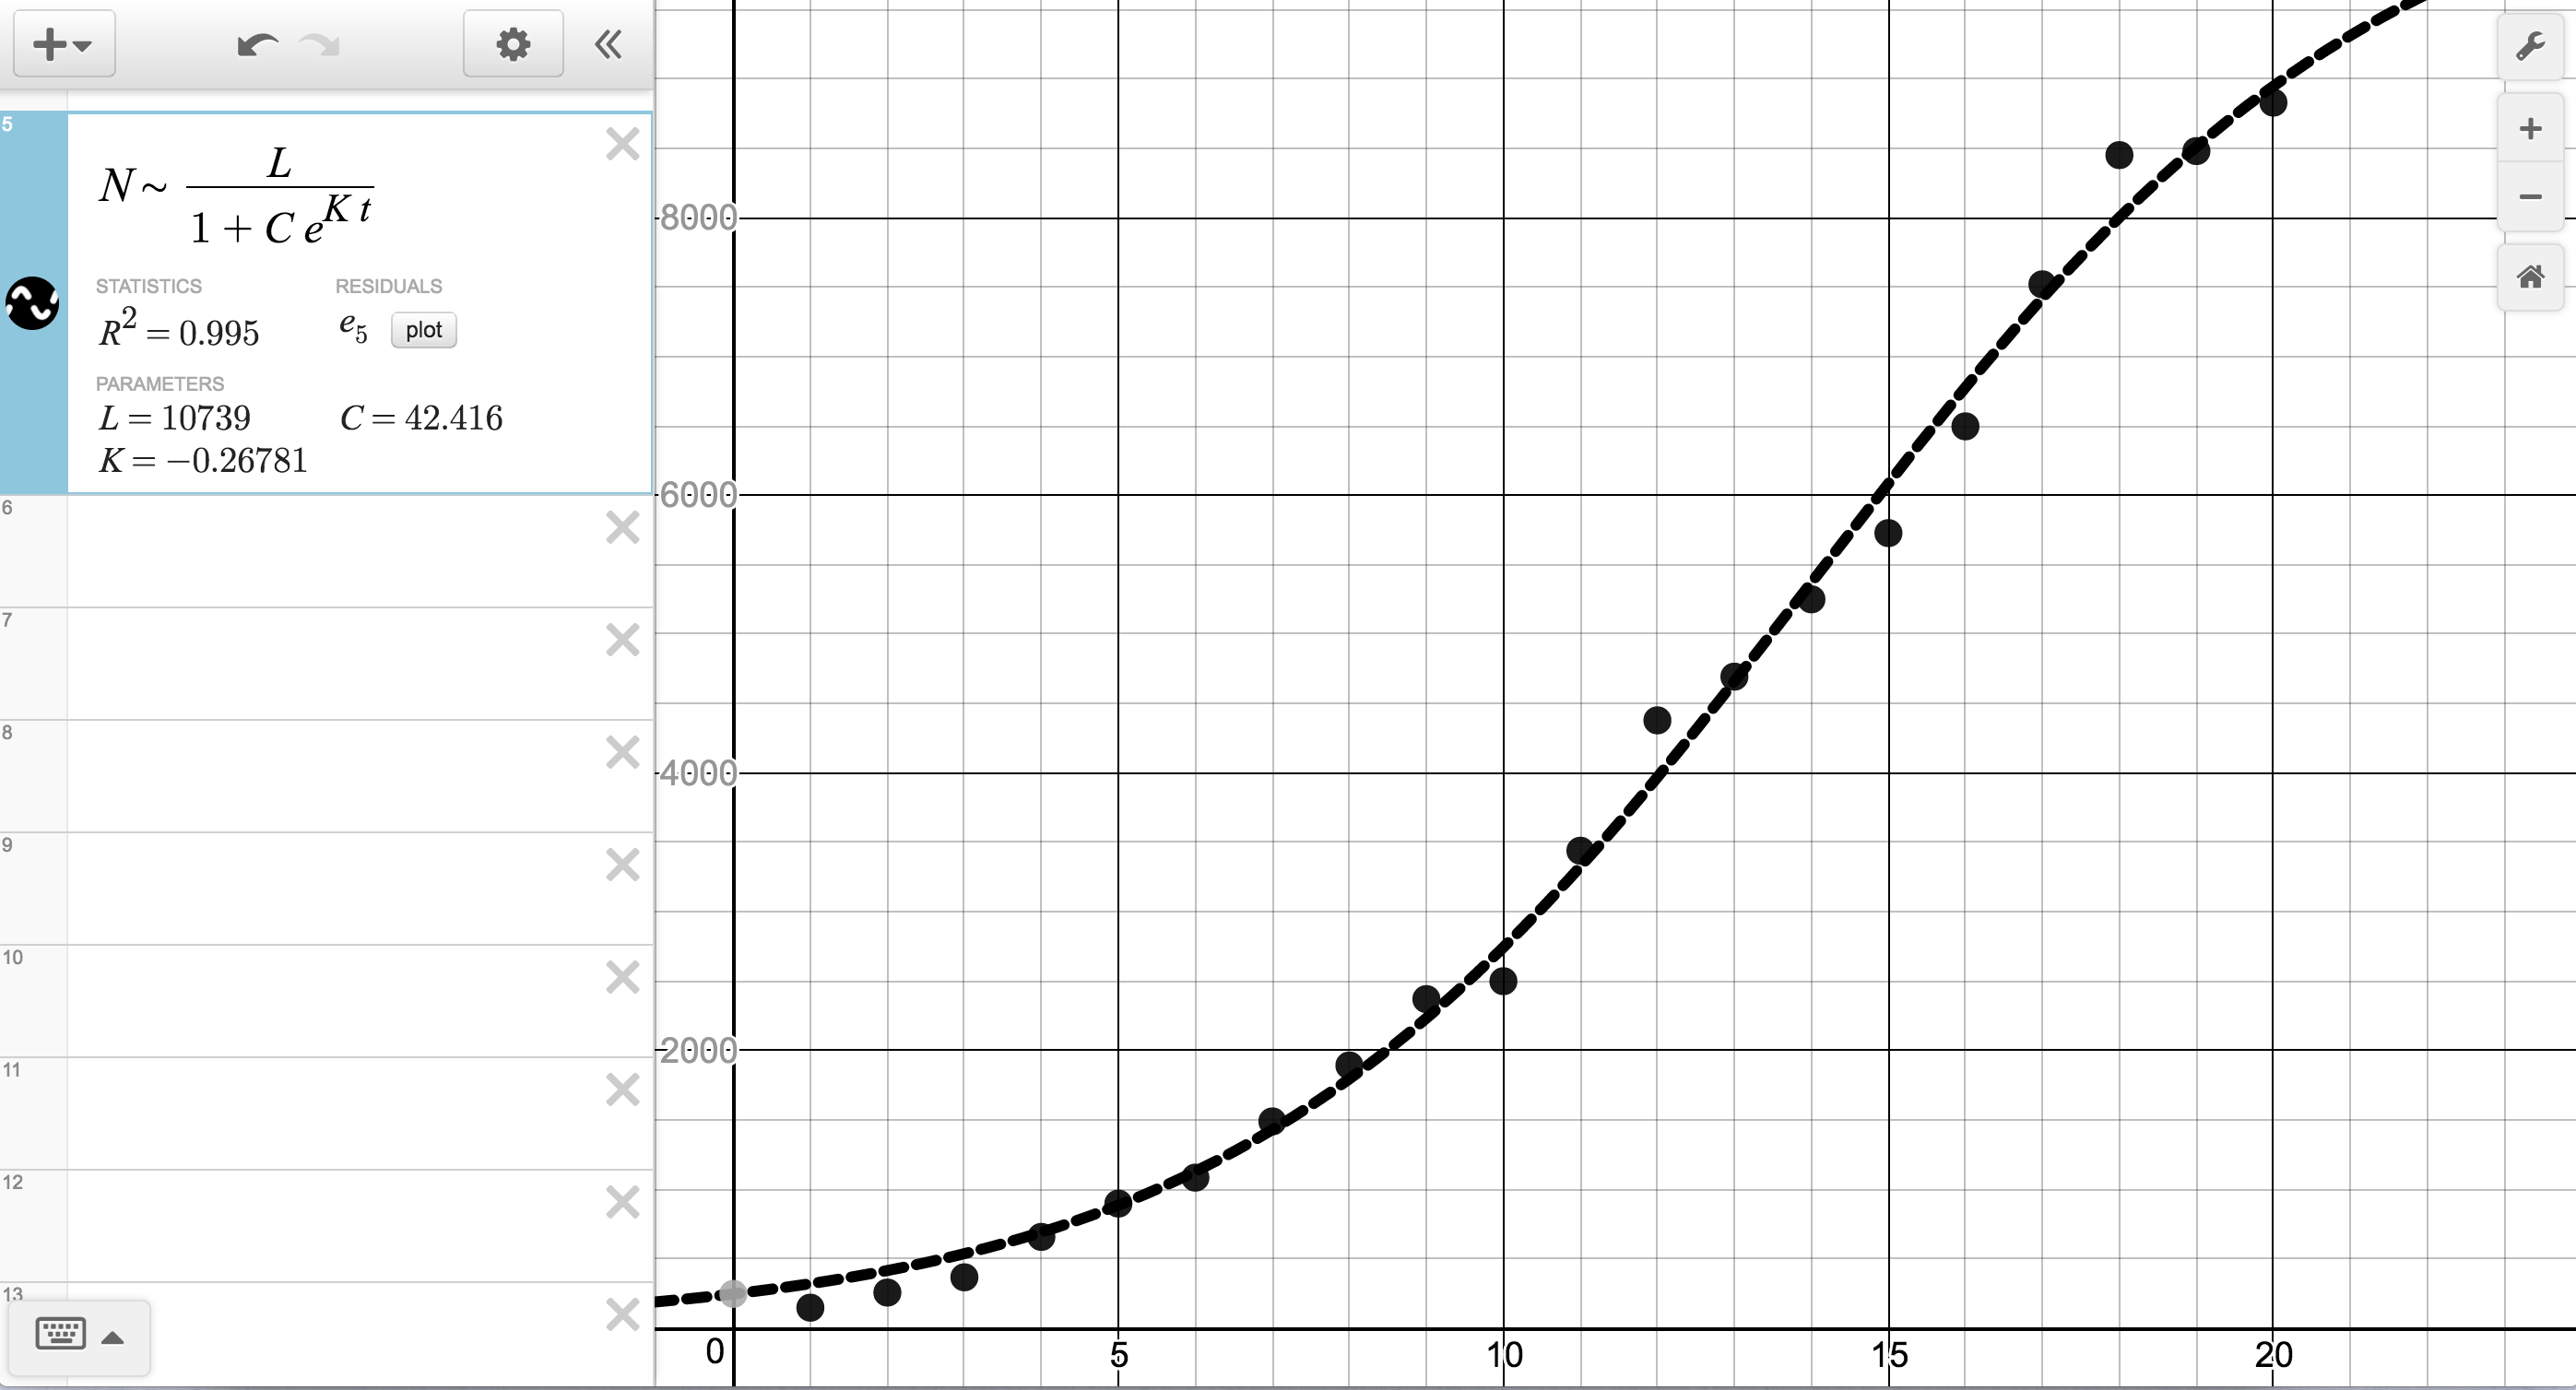
\includegraphics[width=5in]{./ApplicationsofExponentialandLogarithmicFunctionsGraphics/ExpLogAppEx08.jpg} 
 \end{center}



  While the quadratic model also fits extremely well, our logistic model takes into account that only a finite number of people will ever get the flu (according to our model, $L=10,\!739$), whereas the quadratic model predicts no limit to the number of cases. As we have stated several times before in the text, mathematical models, regardless of their sophistication, are just that:  models, and they all have their limitations.\footnote{Speaking of limitations, as of June 3, 2009, there were 19,273 confirmed cases of influenza A (H1N1).  This is well above our prediction of 10,739.  Each time a new report is issued, the data set increases and the model must be recalculated.  We leave this recalculation to the reader.}


\newpage

\subsection{Exercises}

\label{ExercisesforApplicationsofExponentialandLogarithmicFunctions}

For each of the scenarios given in Exercises \ref{basicinterestexfirst} - \ref{basicinterestexlast}, 

\begin{itemize}

\item  Find the amount $A$ in the account as a function of the term of the investment $t$ in years. 

\item  To the nearest cent, determine how much is in the account after $5$, $10$, $30$ and $35$ years.  

\item  To the nearest year, determine how long will it take for the initial investment to double.  

\item  Find and interpret the average rate of change of the amount in the account from the end of
the fourth year to the end of the fifth year, and from the end of the thirty-fourth year to the
end of the thirty-fifth year.  Round your answer to two decimal places.

\end{itemize} 

\begin{enumerate}

\item  $\$500$ is invested in an account which offers $0.75 \%$, compounded monthly. \label{basicinterestexfirst}

\item  $\$500$ is invested in an account which offers $0.75 \%$, compounded continuously.

\item  $\$1000$ is invested in an account which offers $1.25 \%$, compounded monthly.

\item  $\$1000$ is invested in an account which offers $1.25 \%$, compounded continuously.

\item  $\$5000$ is invested in an account which offers $2.125 \%$, compounded monthly.

\item  $\$5000$ is invested in an account which offers $2.125 \%$, compounded continuously. \label{basicinterestexlast}

\setcounter{HW}{\value{enumi}}
\end{enumerate}

\begin{enumerate}
\setcounter{enumi}{\value{HW}}

\item  Look back at your answers to Exercises \ref{basicinterestexfirst} - \ref{basicinterestexlast}. What can be said about the difference between monthly compounding and continuously compounding the interest in those situations?  With the help of your classmates, discuss scenarios where the difference between monthly  and continuously compounded interest would be more dramatic.  Try varying the interest rate, the term of the investment and the principal.  Use computations to support your answer.

\item  How much money needs to be invested now to obtain $\$2000$ in 3 years if the interest rate in a savings account is $0.25 \%$, compounded continuously?  Round your answer to the nearest cent.

\item  How much money needs to be invested now to obtain $\$5000$ in  10 years if the interest rate in a CD is $2.25 \%$, compounded monthly?  Round your answer to the nearest cent.


\item On May, 31, 2009, the Annual Percentage Rate listed at Jeff's bank for regular savings accounts was $0.25\%$ compounded monthly.  Use Equation \ref{compoundinterest} to answer the following.

\begin{enumerate}

\item If $P = 2000$ what is $A(8)$?
\item Solve the equation $A(t) = 4000$ for $t$.
\item What principal $P$ should be invested so that the account balance is \$2000 is three years?

\end{enumerate}

\pagebreak

\item Jeff's bank also offers a 36-month Certificate of Deposit (CD) with an APR of $2.25\%$.

\begin{enumerate}

\item If $P = 2000$ what is $A(8)$?
\item Solve the equation $A(t) = 4000$ for $t$.
\item What principal $P$ should be invested so that the account balance is \$2000 in three years?
\item The Annual Percentage Yield is the \underline{simple} interest rate that returns the same amount of interest after one year as the compound interest does.  With the help of your classmates, compute the APY for this investment.

\end{enumerate}


\item  A finance company offers a promotion on $\$5000$ loans.  The borrower does not have to make any payments for the first three years, however interest will continue to be charged to the loan at $29.9 \%$ compounded continuously.  What amount will be due at the end of the three year period, assuming no payments are made?  If the promotion is extended an additional three years, and no payments are made, what amount would be due?

\item Use Equation \ref{compoundinterest} to show that the time it takes for an investment to double in value does \underline{not} depend on the principal $P$, but rather, depends only on the APR and the number of compoundings per year.  Let $n = 12$ and with the help of your classmates compute the doubling time for a variety of rates $r$.  Then look up the Rule of 72 and compare your answers to what that rule says.  If you're really interested\footnote{Awesome pun!} in Financial Mathematics, you could also compare and contrast the Rule of 72 with the Rule of 70 and the Rule of 69.

\setcounter{HW}{\value{enumi}}
\end{enumerate}

In Exercises \ref{radioactivefirst} - \ref{radioactivelast},  we list some radioactive isotopes and their associated half-lives.  Assume that each decays according to the formula $A(t) = A_{\text{\tiny $0$}}e^{kt}$ where $A_{\text{\tiny $0$}}$ is the initial amount of the material and $k$ is the decay constant. For each isotope:

\begin{itemize}

\item  Find the decay constant $k$.  Round your answer to four decimal places.

\item  Find a function which gives the amount of isotope $A$ which remains after time $t$.  (Keep the units of $A$ and $t$ the same as the given data.)

\item  Determine how long it takes for $90 \%$ of the material to decay.  Round your answer to two decimal places.  (HINT:  If $90 \%$ of the material decays, how much is left?)

\end{itemize}

\begin{enumerate}
\setcounter{enumi}{\value{HW}}

\item  Cobalt 60, used in food irradiation, initial amount 50 grams, half-life of $5.27$ years.  \label{radioactivefirst}

\item  Phosphorus 32, used in agriculture, initial amount 2 milligrams, half-life $14$ days.

\item  Chromium 51, used to track red blood cells, initial amount 75 milligrams, half-life  $27.7$ days.

\item  Americium 241, used in smoke detectors, initial amount 0.29 micrograms, half-life $432.7$ years.

\item  Uranium 235, used for nuclear power, initial amount $1$ kg grams, half-life  $704$ million years. \label{radioactivelast}

\setcounter{HW}{\value{enumi}}
\end{enumerate}

\begin{enumerate}
\setcounter{enumi}{\value{HW}}

\item With the help of your classmates, show that the time it takes for $90 \%$ of each isotope listed in Exercises \ref{radioactivefirst} - \ref{radioactivelast} to decay does not depend on the initial amount of the substance, but rather, on only the decay constant $k$. Find a formula, in terms of $k$ only, to determine how long it takes for $90 \%$ of a radioactive isotope to decay. 


\item In Example \ref{cardepreciationex} in Section \ref{ExponentialFunctions}, the exponential function $V(x) = 25 \left(\frac{4}{5}\right)^{x}$ was used to model the value of a car over time.  Use a change of base formula to rewrite the model in the form $V(t) = 25e^{kt}$.

\item  The Gross Domestic Product (GDP) of the US (in billions of dollars) $t$ years after the year 2000 can be modeled by: \[ G(t) = 9743.77 e^{0.0514t}\]

\begin{enumerate}

\item  Find and interpret $G(0)$.

\item  According to the model, what should have been the GDP in 2007?  In 2010?  (According to the   \href{http://1.usa.gov/iimT40}{\underline{US Department of Commerce}}, the 2007 GDP was $\$14,369.1$ billion and the 2010 GDP was $\$14,657.8$ billion.)

\end{enumerate}

\item  The diameter $D$ of a tumor, in millimeters, $t$ days after it is detected is given by:  \[D(t) = 15e^{0.0277t} \]

\begin{enumerate}

\item  What was the diameter of the tumor when it was originally detected?

\item  How long until the diameter of the tumor doubles?

\end{enumerate}

\item  Under optimal conditions, the growth of a certain strain of \textit{E. Coli} is modeled by the Law of Uninhibited Growth $N(t) = N_{\text{\tiny $0$}} e^{kt}$ where $N_{\text{\tiny $0$}}$ is the initial number of bacteria and $t$ is the elapsed time, measured in minutes. From numerous experiments, it has been determined that the doubling time of this organism is 20 minutes. Suppose 1000 bacteria are present initially.

\begin{enumerate}

\item  Find the growth constant $k$. Round your answer to four decimal places.

\item  Find a function which gives the number of bacteria $N(t)$ after $t$ minutes.

\item  How long until there are 9000 bacteria?  Round your answer to the nearest minute.

\end{enumerate}

\item  Yeast is often used in biological experiments.  A research technician estimates that a sample of yeast suspension contains 2.5 million organisms per cubic centimeter (cc).  Two hours later, she estimates the population density to be 6 million organisms per cc.  Let $t$ be the time elapsed since the first observation, measured in hours.  Assume that the yeast growth follows the Law of Uninhibited Growth $N(t) = N_{\text{\tiny $0$}} e^{kt}$.

\begin{enumerate}

\item  Find the growth constant $k$. Round your answer to four decimal places.

\item  Find a function which gives the number of yeast (in millions) per cc $N(t)$ after $t$ hours.

\item  What is the doubling time for this strain of yeast?

\end{enumerate}


\item  The Law of Uninhibited Growth also applies to situations where an animal is re-introduced into a suitable environment.  Such a case is the reintroduction of wolves to Yellowstone National Park.   According to the \href{http://www.nps.gov/yell/naturescience/wolves.htm}{\underline{National Park Service}}, the wolf population in Yellowstone National Park was 52 in 1996 and 118 in 1999.  Using these data, find a function of the form $N(t) = N_{\text{\tiny $0$}} e^{kt}$  which models the number of wolves $t$ years after 1996.  (Use $t = 0$ to represent the year 1996.  Also, round your value of $k$ to four decimal places.)  According to the model, how many wolves were in Yellowstone in 2002?  (The recorded number is 272.)

\item  \label{PainesvillePopulationTwoPoint} During the early years of a community, it is not uncommon for the population to grow according to the Law of Uninhibited Growth.  According to the Painesville Wikipedia entry, in 1860, the Village of Painesville had a population of 2649.  In 1920, the population was 7272.  Use these two data points to fit a model of the form $N(t) = N_{\text{\tiny $0$}} e^{kt}$ were $N(t)$ is the number of Painesville Residents $t$ years after 1860.  (Use $t = 0$ to represent the year 1860.  Also, round the value of $k$ to four decimal places.)  According to this model, what was the population of Painesville in 2010?  (The 2010 census gave the population as 19,563) What could be some causes for such a vast discrepancy?  For more on this, see Exercise \ref{PainesvillePopulationManyPoints}.

\item  The population of Sasquatch in Bigfoot county is modeled by \[P(t) = \dfrac{120}{1 + 3.167e^{-0.05t}}\] where $P(t)$ is the population of Sasquatch $t$ years after $2010$.

\begin{enumerate}

\item  Find and interpret $P(0)$.

\item  Find the population of Sasquatch in Bigfoot county in 2013 rounded to the nearest Sasquatch.

\item  To the nearest year, when will the population of Sasquatch in Bigfoot county reach 60?  

\item   Find and interpret the end behavior of the graph of $y = P(t)$ analytically. Check your answer using a graphing utility. 

\end{enumerate}

\setcounter{HW}{\value{enumi}}
\end{enumerate}


\begin{enumerate}
\setcounter{enumi}{\value{HW}}

\item  Let $f(x) = \dfrac{10}{1+e^{-x+1}}$.   

\begin{enumerate}

\item From Calculus, we know the inflection point of the graph of $y=f(x)$ is $(1,5)$.  This means the function is increasing the fastest at $x=1$, or, equivalently, the slope at $(1,5)$ is the largest anywhere on the graph.  Graph $y=f(x)$ using a graphing utility and convince yourself of the reasonableness of this claim.

\item Find average rate of change of $f$ over each of the intervals below.  What do you guess the slope of the curve is at $(1,5)$?  Zoom in on the graph near $(1,5)$ to check your guess.

\begin{multicols}{6}

\begin{itemize}

\item $[0.75, 1]$

\item $[0.9, 1]$

\item $[0.99,1]$

\item $[1, 1.01]$

\item $[1, 1.1]$

\item $[1, 1.25]$

\end{itemize}

\end{multicols}

\end{enumerate}

\newpage


\item The half-life of the radioactive isotope Carbon-14 is about 5730 years.  

\begin{enumerate}

\item Use Equation \ref{radioactivedecay} to express the amount of Carbon-14 left from an initial $N$ milligrams as a function of time $t$ in years.

\item What percentage of the original amount of Carbon-14 is left after 20,000 years?

\item If an old wooden tool is found in a cave and the amount of Carbon-14 present in it is estimated to be only 42\% of the original amount, approximately how old is the tool?

\item Radiocarbon dating is not as easy as these exercises might lead you to believe.  With the help of your classmates, research radiocarbon dating and discuss why our model is somewhat over-simplified.  

\end{enumerate}

\item Carbon-14 cannot be used to date inorganic material such as rocks, but there are many other methods of radiometric dating which estimate the age of rocks.  One of them, Rubidium-Strontium dating, uses Rubidium-87 which decays to Strontium-87 with a half-life of 50 billion years.  Use Equation \ref{radioactivedecay} to express the amount of Rubidium-87 left from an initial 2.3 micrograms as a function of time $t$ in \emph{billions} of years.  Research this and other radiometric techniques and discuss the margins of error for various methods with your classmates.

\item  Find and interpret the relative rate of change of  $A(t)$ in Equation \ref{compoundinterest} over the interval $\left[t, t+\frac{1}{n} \right]$.

\item Use Equation \ref{radioactivedecay} to show that $k = -\dfrac{\ln(2)}{h}$ where $h$ is the half-life of the radioactive isotope.

\item A pork roast\footnote{This roast was enjoyed by Jeff and his family on June 10, 2009.  This is real data, folks!} was taken out of a hardwood smoker when its internal temperature had reached $180^{\circ}$F and it was allowed to rest in a $75^{\circ}$F house for 20 minutes after which its internal temperature had dropped to $170^{\circ}$F. 

Assuming that the temperature of the roast follows Newton's Law of Cooling (Equation \ref{newtonslawofcooling}),

\begin{enumerate}

\item Express the temperature $T$ (in $^{\circ}$F) as a function of time $t$ (in minutes).

\item Find the time at which the roast would have dropped to $140^{\circ}$F had it not been eaten. 

\end{enumerate}

\item  \label{pursuitlog} In reference to Exercise \ref{pursuitfurther} in Section \ref{PowerFunctions}, if Fritzy the Fox's speed is the same as Chewbacca the Bunny's speed, Fritzy's pursuit curve is given by

\[y(x) = \frac{1}{4} x^2-\frac{1}{4} \ln(x)-\frac{1}{4}\]

Graph this path for $x > 0$ using a graphing utility.  Describe the behavior of $y$ as $x \rightarrow 0^{+}$ and interpret this physically.

\item \label{explogsappcircuitone} The current $i$ measured in amps in a certain electronic circuit with a constant impressed voltage of 120 volts is given by $i(t) = 2 - 2e^{-10t}$ where $t \geq 0$ is the number of seconds after the circuit is switched on.  Determine the value of $i$ as $t \rightarrow \infty$.  (This is called the \textbf{steady state} current.)


\item If the voltage in the circuit in Exercise \ref{explogsappcircuitone} above is switched off after 30 seconds, the current is given by the piecewise-defined function 

\[i(t) = \left\{ \begin{array}{rcl} 2 - 2e^{-10t} & \mbox{if} & 0 \leq t < 30 \\ [6pt]
\left(2 - 2e^{-300}\right) e^{-10t+300} & \mbox{if} & t \geq 30 \end{array} \right.\]  

With the help of a graphing utility, graph $y = i(t)$ and discuss with your classmates the physical significance of the two parts of the graph $0 \leq t < 30$ and $t \geq 30$.


\item \label{catenary} In Exercise \ref{parabolicbridgecable} in Section \ref{QuadraticFunctions}, we stated that the cable of a suspension bridge formed a parabola but that a free hanging cable did not.  A free hanging cable forms a \underline{catenary} and its basic shape is given by $y = \frac{1}{2}\left(e^{x} + e^{-x}\right)$.  Use a graphing utility to graph this function.  What are its domain and range?  What is its end behavior?  Is it invertible?  How do you think it is related to the function given in Exercise \ref{hyperbolicsine} in Section \ref{ExponentialEquationsandInequalities} and the one given in the answer to Exercise \ref{inversehyptangent} in Section \ref{LogarithmicEquationsandInequalities}?  

When flipped upside down, the catenary makes an arch.  The Gateway Arch in St. Louis, Missouri has the shape \[y = 757.7 - \frac{127.7}{2}\left(e^{\frac{x}{127.7}} + e^{-\frac{x}{127.7}}\right)\] where $x$ and $y$ are measured in feet and $-315 \leq x \leq 315$.  Find the highest point on the arch.

\item \label{APLcatsrevisited} In Exercise \ref{APLcats} in Section \ref{QuadraticFunctions}, we examined the data set given below which showed how two cats and their surviving offspring can produce over 80 million cats in just ten years. Plot $x$ versus $\ln(x)$ as was done on page \pageref{swineflulinearized} using a graphing utility.  

Find a linear model for this new data and comment on its goodness of fit and  find an exponential model for the original data and comment on its goodness of fit.

\medskip

\small

\noindent \begin{tabular}{|l|r|r|r|r|r|r|r|r|r|r|} \hline
Year $x$ & 1 & 2 & 3 & 4 & 5 & 6 & 7 & 8 & 9 & 10 \\ 
\hline 
Number of  & & & & & & & & & & \\
Cats $N(x)$ & 12 & 66 & 382 & 2201 & 12680 & 73041 & 420715 & 2423316 & 13968290 & 80399780 \\ \hline
\end{tabular}

\normalsize

\item \label{LorenzExFollowUp} In Example \ref{LorenzEx} in Section \ref{PowerFunctions}, we fit a power function of the form $L(x) = a x^{p}$ to a set of data, $(x, L(x))$.  In this exercise, we use logs to linearize this data using the same methods presented on page \pageref{swineflulinearized}, but with a slight difference in interpretation.

\begin{enumerate}

\item  Starting with $L(x) = a x^{p}$, take natural logs of both sides of the equation and use log properties to rewrite the resulting equation as:  $\ln(L(x)) = p \ln(x) + \ln(a)$.  

\item  Use a graphing utility to find a least squares regression line using the data $(\ln(x), \ln(L(x)))$.   

NOTE:  In this situation, we are plotting $\ln(x)$ versus $\ln(L(x))$ instead of $x$ versus $\ln(L(x))$.  

\item  \label{newlorenzepart} Find the slope $p$ of the regression line and the intercept $\ln(a)$.  Use these to construct a model of the form $L(x) = a x^{p}$.   Find and interpret $L(90)$.

\item   Graph both the model obtained in Example \ref{LorenzEx} and the model obtained in part \ref{newlorenzepart} along with the original data.  What do you notice?

\end{enumerate}

\item  \label{PainesvillePopulationManyPoints} This exercise is a follow-up to Exercise \ref{PainesvillePopulationTwoPoint} which more thoroughly explores the population growth of Painesville, Ohio.  According to \href{http://en.wikipedia.org/wiki/Painesville}{\underline{Wikipedia}}, the population of Painesville, Ohio is given by


\noindent \begin{tabular}{|l|r|r|r|r|r|r|r|r|r|r|} \hline
Year $t$ & 1860 & 1870 & 1880 & 1890 & 1900 & 1910 & 1920 & 1930 & 1940 & 1950 \\ \hline 
Population& 2649 & 3728 & 3841 & 4755 & 5024 & 5501 & 7272 & 10944 & 12235 & 14432 \\ \hline
\end{tabular}

\noindent \begin{tabular}{|l|r|r|r|r|r|} \hline
Year $t$ & 1960 & 1970 & 1980 & 1990 & 2000 \\ \hline 
Population& 16116 & 16536 & 16351 & 15699 & 17503 \\ \hline
\end{tabular}

\begin{enumerate}

\item  Use a graphing utility to perform an exponential regression on the data from 1860 through 1920 only, letting $t = 0$ represent the year 1860 as before.  How does this model compare with the model you found in Exercise \ref{PainesvillePopulationTwoPoint}?   Use the graphing utility's exponential model to predict the population in 2010.   (The 2010 census gave the population as 19,563)

\item  The logistic model fit to \emph{all} of the given data points for the population of Painesville $t$ years after 1860 (again, using $t = 0$ as 1860) is \[ P(t) = \dfrac{18691}{1+9.8505e^{-0.03617t}} \] According to this model, what should the population of Painesville have been in 2010?  (The 2010 census gave the population as 19,563.) What is the population limit of Painesville?

\end{enumerate}

\item  According to \href{http://www.ohiobiz.com/census/Lake.pdf}{\underline{OhioBiz}}, the census data for Lake County, Ohio is as follows:

\small
\noindent \begin{tabular}{|l|r|r|r|r|r|r|r|r|r|r|} \hline
Year $t$ & 1860 & 1870 & 1880 & 1890 & 1900 & 1910 & 1920 & 1930 & 1940 & 1950 \\ \hline 
Population& 15576 & 15935 & 16326 & 18235 & 21680 & 22927 & 28667 & 41674 & 50020 & 75979 \\ \hline
\end{tabular}

\noindent \begin{tabular}{|l|r|r|r|r|r|} \hline
Year $t$ & 1960 & 1970 & 1980 & 1990 & 2000 \\ \hline 
Population& 148700 & 197200 & 212801 & 215499 & 227511 \\ \hline
\end{tabular}

\normalsize

\begin{enumerate}

\item  Use a graphing utility to fit a logistic model to these data with $x = 0$ representing the year 1860. 

\item  Graph the data and your model using a graphing utility to judge the reasonableness of the fit.

\item  Use this model to estimate the population of Lake County in 2010.  (The 2010 census gave the population to be 230,041.)

\item  According to your model, what is the population limit of Lake County, Ohio?

\end{enumerate}


\item According to \href{http://www.facebook.com/press/info.php?timeline}{\underline{facebook}}, the number of active users of facebook has grown significantly since its initial launch from a Harvard dorm room in February 2004. The chart below has the approximate number $U(x)$ of active users, in \underline{millions}, $x$ months after February 2004.  For example, the first entry $(10, 1)$ means that there were $1$ million active users in December 2004 and the last entry $(77, 500)$ means that there were $500$ million active users in July 2010.

\medskip
\small
\noindent \begin{tabular}{|l|r|r|r|r|r|r|r|r|r|r|r|r|r|r|} \hline
Month $x$ & 10 & 22 & 34 & 38 & 44 & 54 & 59 & 60 & 62 & 65 & 67 & 70 & 72 & 77 \\ \hline 
Active Users in & & & & & & & & & & & & & & \\
Millions $U(x)$ & 1 & 5.5 & 12 & 20 & 50 & 100 & 150 & 175 & 200 & 250 & 300 & 350 & 400 & 500\\ \hline
\end{tabular}
\normalsize
\medskip

  With the help of your classmates, find a model for this data.


\item Each Monday during the registration period before the Fall Semester at LCCC, the Enrollment Planning Council gets a report prepared by the data analysts in Institutional Effectiveness and Planning.\footnote{Thanks to Dr. Wendy Marley and her staff for this data and Dr. Marcia Ballinger for the permission to use it  in this problem.}  While the ongoing enrollment data is analyzed in many different ways, we shall focus only on the overall headcount.  Below is a chart of the enrollment data for Fall Semester 2008.  It starts 21 weeks before ``Opening Day'' and ends on ``Day 15'' of the semester, but we have relabeled the top row to be $x = 1$ through $x = 24$ so that the math is easier.  (Thus, $x = 22$ is Opening Day.)


\noindent \begin{tabular}{|l|r|r|r|r|r|r|r|r|} \hline
Week $x$ & 1 & 2 & 3 & 4 & 5 & 6 & 7 & 8 \\ \hline 
Total  & & & & & & & & \\
Headcount & 1194 & 1564 & 2001 & 2475 & 2802 & 3141 & 3527 & 3790 \\ \hline
\end{tabular}

\medskip

\noindent \begin{tabular}{|l|r|r|r|r|r|r|r|r|} \hline
Week $x$ & 9 & 10 & 11 & 12 & 13 & 14 & 15 & 16 \\ \hline 
Total  & & & & & & & & \\
Headcount & 4065 & 4371 & 4611 & 4945 & 5300 & 5657 & 6056 & 6478 \\ \hline
\end{tabular}

\medskip

\noindent \begin{tabular}{|l|r|r|r|r|r|r|r|r|} \hline
Week $x$ & 17 & 18 & 19 & 20 & 21 & 22 & 23 & 24\\ \hline 
Total  & & & & & & & & \\
Headcount & 7161 & 7772 & 8505 & 9256 & 10201 & 10743 & 11102 & 11181 \\ \hline
\end{tabular}

\medskip

With the help of your classmates, find a model for this data.  Unlike most of the phenomena we have studied in this section, there is no single differential equation which governs the enrollment growth.  Thus there is no scientific reason to rely on a logistic function even though the data plot may lead us to that model.  What are some factors which influence enrollment at a community college and how can you take those into account mathematically?  

\item When we wrote this exercise, the Enrollment Planning Report for Fall Semester 2009 had only 10 data points for the first 10 weeks of the registration period.  Those numbers are given below.  

\noindent \begin{tabular}{|l|r|r|r|r|r|r|r|r|r|r|} \hline
Week $x$ & 1 & 2 & 3 & 4 & 5 & 6 & 7 & 8 & 9 & 10 \\ \hline 
Total  & & & & & & & & & & \\
Headcount & 1380 & 2000 & 2639 & 3153 & 3499 & 3831 & 4283 & 4742 & 5123 & 5398 \\ \hline
\end{tabular}

With the help of your classmates, find a model for this data and make a prediction for the Opening Day enrollment as well as the Day 15 enrollment.  (WARNING: The registration period for 2009 was one week shorter than it was in 2008 so Opening Day would be $x = 21$ and Day 15 is $x = 23$.)


\end{enumerate}

\newpage

\subsection{Answers}

\begin{enumerate}

\item \begin{itemize}  \item $A(t) = 500\left(1 + \frac{0.0075}{12}\right)^{12t}$ 

\item $A(5) \approx \$ 519.10$, $A(10) \approx \$ 538.93$, $A(30) \approx \$ 626.12$, $A(35) \approx \$ 650.03$ 

\item It will take approximately $92$ years for the investment to double.

\item  The average rate of change from the end of the fourth year to the end of the fifth year is approximately $3.88$.  This means that the investment is growing at an average rate of $\$3.88$ per year at this point.  The average rate of change from the end of the thirty-fourth year to the end of the thirty-fifth year is approximately $4.85$.  This means that the investment is growing at an average rate of $\$4.85$ per year at this point. 

\end{itemize}

\item \begin{itemize}  \item $A(t) = 500e^{0.0075t}$ 

\item $A(5) \approx \$ 519.11$, $A(10) \approx \$ 538.94$, $A(30) \approx \$ 626.16$, $A(35) \approx \$ 650.09$ 

\item It will take approximately $92$ years for the investment to double.

\item  The average rate of change from the end of the fourth year to the end of the fifth year is approximately $3.88$.  This means that the investment is growing at an average rate of $\$3.88$ per year at this point.  The average rate of change from the end of the thirty-fourth year to the end of the thirty-fifth year is approximately $4.86$.  This means that the investment is growing at an average rate of $\$4.86$ per year at this point. 

\end{itemize}

\item \begin{itemize}  \item $A(t) = 1000\left(1 + \frac{0.0125}{12}\right)^{12t}$ 

\item $A(5) \approx \$ 1064.46$, $A(10) \approx \$ 1133.07$, $A(30) \approx \$ 1454.71$, $A(35) \approx \$ 1548.48$ 

\item  It will take approximately $55$ years for the investment to double.

\item  The average rate of change from the end of the fourth year to the end of the fifth year is approximately $13.22$.  This means that the investment is growing at an average rate of $\$13.22$ per year at this point.  The average rate of change from the end of the thirty-fourth year to the end of the thirty-fifth year is approximately $19.23$.  This means that the investment is growing at an average rate of $\$19.23$ per year at this point. 

\end{itemize}



\item \begin{itemize}  \item $A(t) = 1000e^{0.0125t}$ 

\item $A(5) \approx \$ 1064.49$, $A(10) \approx \$ 1133.15$, $A(30) \approx \$ 1454.99$, $A(35) \approx \$ 1548.83$ 

\item It will take approximately $55$ years for the investment to double.

\item  The average rate of change from the end of the fourth year to the end of the fifth year is approximately $13.22$.  This means that the investment is growing at an average rate of $\$13.22$ per year at this point.  The average rate of change from the end of the thirty-fourth year to the end of the thirty-fifth year is approximately $19.24$.  This means that the investment is growing at an average rate of $\$19.24$ per year at this point. 

\end{itemize}

\pagebreak

\item \begin{itemize}  \item $A(t) = 5000\left(1 + \frac{0.02125}{12}\right)^{12t}$ 

\item $A(5) \approx \$ 5559.98$, $A(10) \approx \$ 6182.67$, $A(30) \approx \$ 9453.40$, $A(35) \approx \$ 10512.13$ 

\item  It will take approximately $33$ years for the investment to double.

\item  The average rate of change from the end of the fourth year to the end of the fifth year is approximately $116.80$.  This means that the investment is growing at an average rate of $\$116.80$ per year at this point.  The average rate of change from the end of the thirty-fourth year to the end of the thirty-fifth year is approximately $220.83$.  This means that the investment is growing at an average rate of $\$220.83$ per year at this point. 

\end{itemize}



\item \begin{itemize}  \item $A(t) = 5000e^{0.02125t}$ 

\item $A(5) \approx \$ 5560.50$, $A(10) \approx \$ 6183.83$, $A(30) \approx \$ 9458.73$, $A(35) \approx \$ 10519.05$ 

\item  It will take approximately $33$ years for the investment to double.

\item  The average rate of change from the end of the fourth year to the end of the fifth year is approximately $116.91$.  This means that the investment is growing at an average rate of $\$116.91$ per year at this point.  The average rate of change from the end of the thirty-fourth year to the end of the thirty-fifth year is approximately $221.17$.  This means that the investment is growing at an average rate of $\$221.17$ per year at this point. 

\end{itemize}

\setcounter{HW}{\value{enumi}}
\end{enumerate}

\begin{enumerate}
\setcounter{enumi}{\value{HW}}

\addtocounter{enumi}{1}

\item  $P = \frac{2000}{e^{0.0025 \cdot 3}} \approx \$ 1985.06$

\item  $P = \frac{5000}{\left(1 + \frac{0.0225}{12}\right)^{12 \cdot 10}} \approx \$ 3993.42$

\item \begin{enumerate}

\item $A(8) = 2000\left(1 + \frac{0.0025}{12}\right)^{12 \cdot 8} \approx \$2040.40$
\item $t = \dfrac{\ln(2)}{12 \ln\left(1 + \frac{0.0025}{12}\right)} \approx 277.29$ years
\item $P = \dfrac{2000}{\left(1 + \frac{0.0025}{12}\right)^{36}} \approx \$1985.06$

\end{enumerate}

\item \begin{enumerate}

\item $A(8) = 2000\left(1 + \frac{0.0225}{12}\right)^{12 \cdot 8} \approx \$2394.03$
\item $t = \dfrac{\ln(2)}{12 \ln\left(1 + \frac{0.0225}{12}\right)} \approx 30.83$ years
\item $P = \dfrac{2000}{\left(1 + \frac{0.0225}{12}\right)^{36}} \approx \$1869.57$
\item $\left(1 + \frac{0.0225}{12}\right)^{12} \approx 1.0227$ so the APY is 2.27\%

\end{enumerate}

\item  $A(3) = 5000e^{0.299 \cdot 3} \approx \$12,226.18$,  $A(6) = 5000e^{0.299 \cdot 6} \approx \$30,067.29$

\setcounter{HW}{\value{enumi}}
\end{enumerate}


\begin{multicols}{2}
\begin{enumerate}
\setcounter{enumi}{\value{HW}}
\addtocounter{enumi}{1}

\item  \begin{itemize}  \item $k = \frac{\ln(1/2)}{5.27} \approx -0.1315$

\item $A(t) = 50e^{-0.1315t}$

\item  $t = \frac{\ln(0.1)}{-0.1315} \approx 17.51$ years.

\end{itemize}



\item  \begin{itemize}  \item $k = \frac{\ln(1/2)}{14} \approx -0.0495$

\item $A(t) = 2e^{-0.0495t}$

\item  $t = \frac{\ln(0.1)}{-0.0495} \approx 46.52$ days.

\end{itemize}

\setcounter{HW}{\value{enumi}}
\end{enumerate}
\end{multicols}

\begin{multicols}{2}
\begin{enumerate}
\setcounter{enumi}{\value{HW}}


\item  \begin{itemize}  \item $k = \frac{\ln(1/2)}{27.7} \approx -0.0250$

\item $A(t) = 75e^{-0.0250t}$

\item  $t = \frac{\ln(0.1)}{-0.025} \approx 92.10$ days.

\end{itemize}

\item  \begin{itemize}  \item $k = \frac{\ln(1/2)}{432.7} \approx -0.0016$

\item $A(t) = 0.29e^{-0.0016t}$

\item  $t = \frac{\ln(0.1)}{-0.0016} \approx 1439.11$ years.

\end{itemize}


\setcounter{HW}{\value{enumi}}
\end{enumerate}
\end{multicols}

\begin{enumerate}
\setcounter{enumi}{\value{HW}}

\item  \begin{itemize}  \item $k = \frac{\ln(1/2)}{704} \approx -0.0010$

\item $A(t) = e^{-0.0010t}$

\item $t = \frac{\ln(0.1)}{-0.0010} \approx 2302.58$ million years, or $2.30$ billion years.

\end{itemize}


\setcounter{HW}{\value{enumi}}
\end{enumerate}

\begin{multicols}{2}
\begin{enumerate}
\setcounter{enumi}{\value{HW}}


\item  $t = \frac{\ln(0.1)}{k} = -\frac{\ln(10)}{k}$

\item $V(t) = 25e^{\ln\left(\frac{4}{5}\right)t} \approx 25e^{-0.22314355t}$

\setcounter{HW}{\value{enumi}}
\end{enumerate}
\end{multicols}


\begin{enumerate}
\setcounter{enumi}{\value{HW}}


\item \begin{enumerate}  \item  $G(0) = 9743.77$  This means that the GDP of the US in 2000 was $\$9743.77$ billion dollars.

\item  $G(7) = 13963.24$ and $G(10) = 16291.25$, so the model predicted a GDP of $\$ 13,963.24$ billion in 2007 and $\$ 16,291.25$ billion in 2010. 

\end{enumerate}

\item \begin{enumerate} \item $D(0) = 15$, so the tumor was 15 millimeters in diameter when it was first detected.

\item  $t = \frac{\ln(2)}{0.0277} \approx 25$ days.

\end{enumerate}

\setcounter{HW}{\value{enumi}}
\end{enumerate}

\begin{multicols}{2}
\begin{enumerate}
\setcounter{enumi}{\value{HW}}

\item  \begin{enumerate} \item  $k = \frac{\ln(2)}{20} \approx 0.0346$

\item  $N(t) = 1000e^{0.0346 t}$

\item  $t = \frac{\ln(9)}{0.0346} \approx 63$ minutes

\end{enumerate}

\item  \begin{enumerate} \item  $k = \frac{1}{2}\frac{\ln(6)}{2.5} \approx 0.4377$

\item  $N(t) = 2.5e^{0.4377 t}$

\item  $t = \frac{\ln(2)}{0.4377} \approx 1.58$ hours

\end{enumerate}

\setcounter{HW}{\value{enumi}}
\end{enumerate}
\end{multicols}

\begin{enumerate}
\setcounter{enumi}{\value{HW}}


\item  $N_{\text{\tiny $0$}} = 52$,  $k = \frac{1}{3} \ln\left( \frac{118}{52}\right) \approx 0.2731$, $N(t) = 52e^{0.2731t}$.  $N(6) \approx 268$. 

\item  $N_{\text{\tiny $0$}} = 2649$,  $k = \frac{1}{60} \ln\left( \frac{7272}{2649}\right) \approx 0.0168$, $N(t) = 2649e^{0.0168t}$.  $N(150) \approx 32923$, so the population of Painesville in 2010 based on this model would have been 32,923.



\item  \begin{enumerate}  \item  $P(0) = \frac{120}{4.167} \approx 29$.  There are 29 Sasquatch in Bigfoot County in 2010.

\item  $P(3) = \frac{120}{1+3.167e^{-0.05(3)}} \approx 32$ Sasquatch.

\item  $t = 20 \ln(3.167) \approx 23$ years.

\item  As $t \rightarrow \infty$, $P(t) \rightarrow 120$.  As time goes by, the Sasquatch Population in Bigfoot County will approach 120.  Graphically,  $y = P(x)$ has a horizontal asymptote $y=120$.

\end{enumerate}

\item 

\begin{enumerate}

\addtocounter{enumii}{1}

\item The average rates of change are listed in order below. They suggest  slope at $(1,5)$ is $2.5$.  

\begin{multicols}{6}

\begin{itemize}

\item $\approx 2.487$

\item $\approx 2.498$

\item $\approx 2.500$

\item $\approx 2.500$

\item $\approx 2.498$

\item$\approx 2.487$

\end{itemize}

\end{multicols}

\end{enumerate}

\pagebreak

\item \begin{enumerate}

\item $A(t) = Ne^{-\left(\frac{\ln(2)}{5730}\right)t} \approx Ne^{-0.00012097t}$
\item $A(20000) \approx 0.088978 \cdot N$ so about 8.9\% remains
\item $t \approx \dfrac{\ln(.42)}{-0.00012097} \approx 7171$ years old

\end{enumerate}

\item $A(t) = 2.3e^{-0.0138629t}$

\item  The relative rate of change of $A(t)$ over $\left[t, t+\frac{1}{n} \right]$ is $\frac{r}{n}$ which is the annual percentage rate divided by the number of compoundings per year -- that is,  the percentage growth rate over one compounding.

\addtocounter{enumi}{1}

\item \begin{enumerate}

\item $T(t) = 75 + 105e^{-0.005005t}$

\item The roast would have cooled to $140^{\circ}$F in about 95 minutes.

\end{enumerate}

\item From the graph, it appears that as $x \rightarrow 0^{+}$, $y \rightarrow \infty$.  This is due to the presence of the $\ln(x)$ term in the function.  This means that Fritzy will never catch Chewbacca, which makes sense since Chewbacca has a head start and Fritzy only runs as fast as he does.

\begin{center}

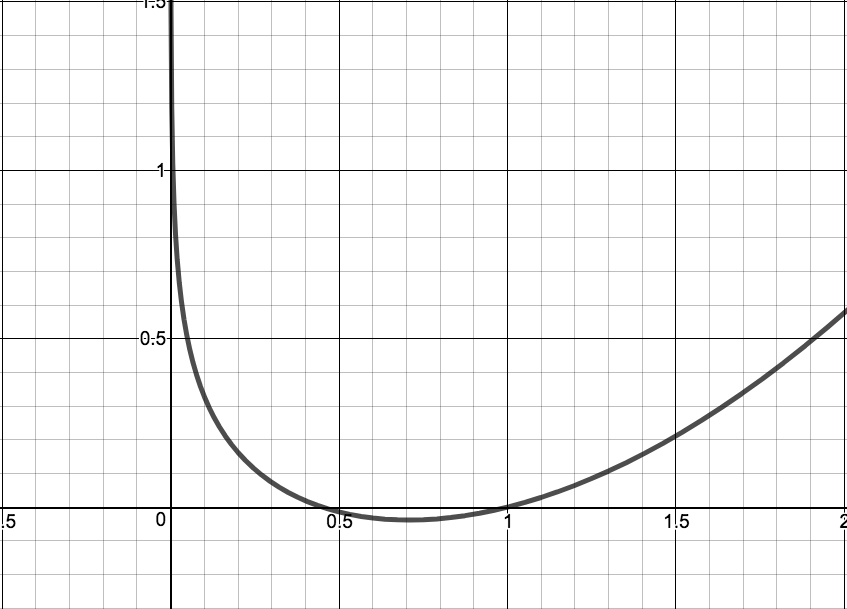
\includegraphics[height=1.5in]{./ApplicationsofExponentialandLogarithmicFunctionsGraphics/PURSUIT03.jpg}

\smallskip

$y(x) = \frac{1}{4} x^2-\frac{1}{4} \ln(x)-\frac{1}{4}$

\end{center}

\item The steady state current is 2 amps.

\addtocounter{enumi}{1}

\item  630 feet.

\item The linear regression on the data below is $y = 1.74899x + 0.70739$ with $r^{2} \approx 0.999995$.  

This is an excellent fit.

\scriptsize

\noindent \begin{tabular}{|l|r|r|r|r|r|r|r|r|r|r|} \hline
$x$ & 1 & 2 & 3 & 4 & 5 & 6 & 7 & 8 & 9 & 10 \\ 
\hline 
$\ln(N(x))$ & 2.4849 & 4.1897 & 5.9454 & 7.6967 & 9.4478 & 11.1988 & 12.9497 & 14.7006 & 16.4523 & 18.2025 \\ \hline
\end{tabular}

\normalsize

$N(x) = 2.02869(5.74879)^{x} = 2.02869e^{1.74899x}$ with $r^{2} \approx 0.999995$.  This is also an excellent fit and corresponds to our linearized model because $\ln(2.02869) \approx 0.70739$.

\item  \begin{enumerate}
\addtocounter{enumii}{1}

\item  The linearized model is: $\ln(L(x)) \approx 2.106 \ln(x) - 5.268$ with an $r^2 \approx  0.9914$.

\item  $L(x) = 0.005154 x^{2.106}$.  $L(90) \approx 67.3$ meaning the bottom $90 \%$ of wage earners take home $67.3 \%$ of the total national income.  Said differently, according to this model, the top $10 \%$ of wage earners take home $32.7 \%$ of the total national income. 



\item  We graph our answer to Example \ref{LorenzEx} in Section \ref{PowerFunctions}, $L(x) = 0.00027901x^{2.7738}$, below on the left.  Below on the right is the model we derived in this exercise. 

\begin{center}

\begin{tabular}{cc}

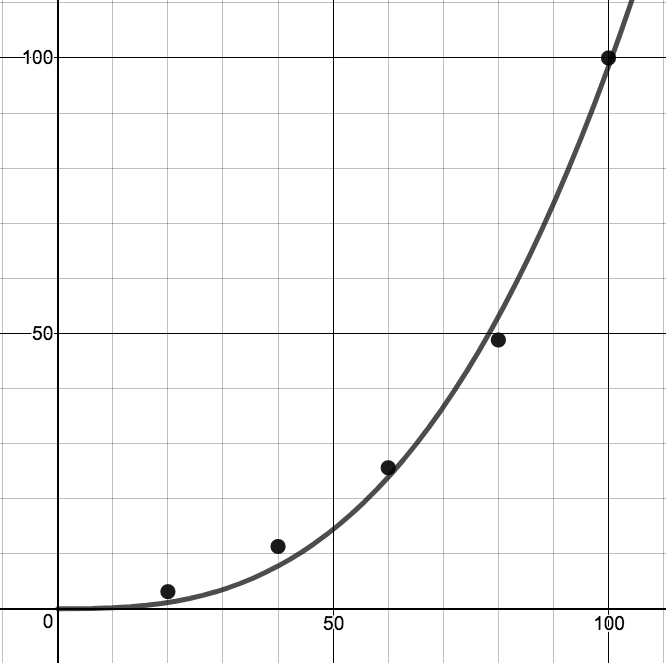
\includegraphics[height=1.5in]{./ApplicationsofExponentialandLogarithmicFunctionsGraphics/OldLorenzModel.jpg}  &

\hspace{1in}

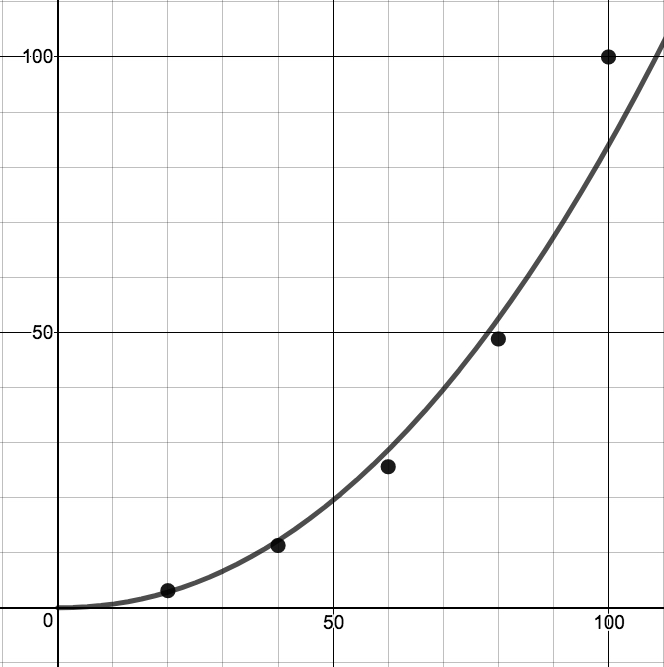
\includegraphics[height=1.5in]{./ApplicationsofExponentialandLogarithmicFunctionsGraphics/NewLorenzModel.jpg}  \\

 $L(x) = 0.00027901x^{2.7738}$

&

\hspace{1in}
$L(x) = 0.005154 x^{2.106}$ \\

\end{tabular}

\end{center}

\end{enumerate}


\item  \begin{enumerate}  \item   We get:  $y = 2895.06 (1.0147)^{x}$.  Graphing this along with our answer from Exercise \ref{PainesvillePopulationTwoPoint} over the interval $[0,60]$ shows that they are pretty close. From this model, $y(150) \approx 25840$ which once again overshoots the actual data value.

\item $P(150) \approx 18717$, so this model predicts 17,914 people in Painesville in 2010, a more conservative number than was recorded in the 2010 census.  As $t \rightarrow \infty$, $P(t) \rightarrow 18691$.  So the limiting population of Painesville based on this model is 18,691 people.

\enlargethispage{\baselineskip}

\end{enumerate}

\item \begin{enumerate}  \item  $y = \dfrac{242526}{1+874.63e^{-0.07113x}}$, where $x$ is the number of years since 1860.

\item  The plot of the data and the curve is below.

\centerline{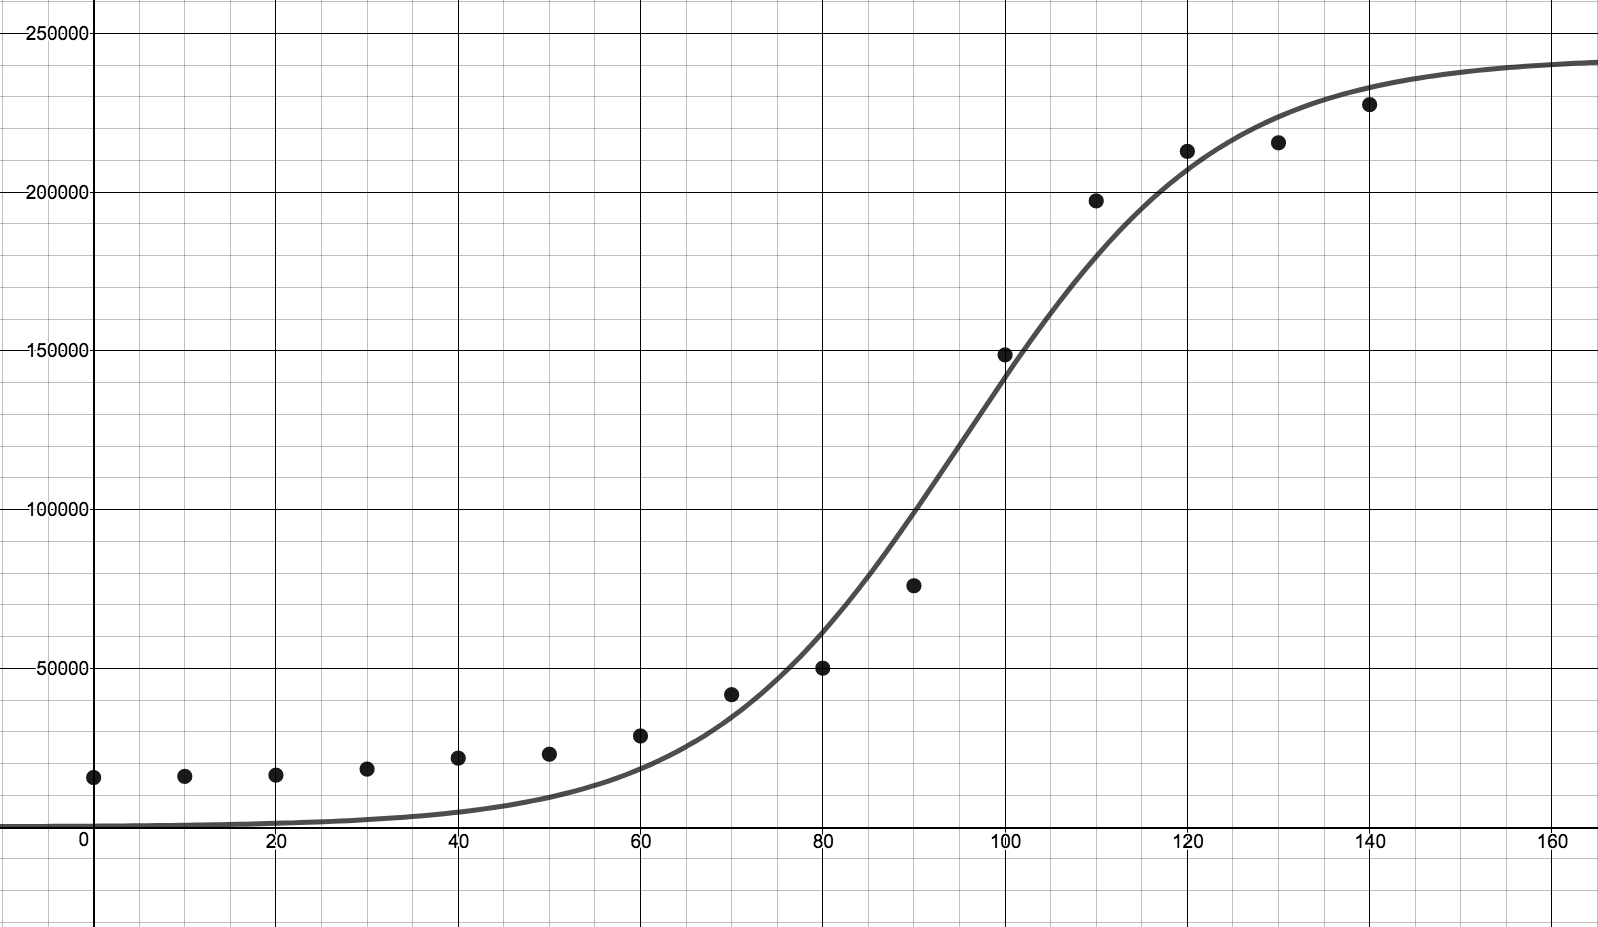
\includegraphics[height=2in]{./ApplicationsofExponentialandLogarithmicFunctionsGraphics/LAKECOUNTYLOGISTIC.jpg}} 

\item  $y(140) \approx 232884$, so this model predicts 232,884 people in Lake County in 2010.

\item  As $x \rightarrow \infty$, $y \rightarrow 242526$, so the limiting population of Lake County based on this model is 242,526 people.

\end{enumerate}

\end{enumerate}


\closegraphsfile
\end{comment}


\end{document}